\documentclass[11pt, a4paper]{article}
\usepackage[utf8]{inputenc}
\usepackage[margin=1in]{geometry} %Sets proper 1-inch margins. 
\usepackage{amsmath} %Only load this if you are using math/equations.
\usepackage{graphicx} %Only need to call this if inserting images.
\usepackage{caption} %Only need to call this if inserting captions.
\usepackage{float} %Allows the use of the [H] specifier. 
\graphicspath{{../../assets/final_plots/}} %Sets the working directory for images.
\usepackage[colorlinks,citecolor=blue,linkcolor=blue,urlcolor=blue]{hyperref} %Allows for the embedding of urls. 
\usepackage{listings}
\lstset{%
   breaklines=true
}

\usepackage{natbib}
\usepackage{longtable}
\usepackage{lscape}
\usepackage{blindtext}
\usepackage{xcolor}
\usepackage{rotating}
\usepackage{tabularx}
\usepackage{booktabs}

\newcommand{\comment}[1]{}

\usepackage{fancyhdr}
\pagestyle{fancy}
\fancyhf{}
\rhead{MDS Capstone}
\lhead{\thepage}

\begin{document}
\begin{center}
\textsc{A Report} \par
\small{\textsc{For the}} \par
\Large{\textsc{SEGMENTATION OF STATISTICS CANADA’S PROXIMITY MEASURES}}
\par
\vspace{0.917 pc} %Creates a paragraph line break. 
\par
\normalsize{ }

\thispagestyle{empty}

\vspace{8 pc} %Creates a paragraph line break. 


\par
June 2023	
\par
\vspace{8pc}

Ricky Heinrich \par
Noman Mohammad \par
Avishek Saha \par 
Jonah Edmundson


%\vspace{0.917 pc} %Creates a paragraph line break. 
%\vspace{0.917 pc} %Creates a paragraph line break. 
\par
\vfill
\thispagestyle{empty}
\par
\noindent\small{Statistics Canada Liaison - Jérôme Blanchet, Bjenk Ellefsen}
\par
\noindent\small{UBCO Project Supervisor - His Excellency Dr. Firas Moosvi}
\par
\vspace{2pc}
\par
\noindent\tiny{In compliance with the Capstone Project requirements of the MDS program at the University of British Columbia - Okanagan.}
\end{center}
\normalsize

\pagebreak



\thispagestyle{empty}
\setcounter{tocdepth}{2} %toc depth 
\tableofcontents
\thispagestyle{empty}

\pagebreak
\thispagestyle{empty}
\listoffigures
\thispagestyle{empty}

\vspace{2pc}

\pagebreak
\thispagestyle{empty}
%\small{\listoftables}
\listoftables
\pagebreak


%%%%%%%%%%%%%%%%%%%%%%%%%%%%%%%%%%%%%%%%
\section{Introduction}
%%%%%%%%%%%%%%%%%%%%%%%%%%%%%%%%%%%%%%%%
\par

\setcounter{page}{1}

\normalsize
Each individual lives somewhere and inhabits physical space. Unless one lives completely removed from others, amenities such as schools, places of employment, and healthcare facilities are usually present in the built environment. These amenities serve to make residents’ lives better, and their distribution is often the result of careful policy and planning by governing bodies. Like people, they inhabit physical space, and not everybody is equidistant from them. As Alasia et al. (2021) outline, ``having physical access to basic services and amenities is a key determinant of social inclusion, their capacity to meet basic needs, and their ability to fully participate in social and economic development.'' Therefore, it is imperative for these governing bodies to make deliberate, well-informed decisions as to the location of new amenities and services.
\par
The Proximity Measure Database (PMD) developed by the Data Exploration and Integration Lab (DEIL) at Statistics Canada serves to provide a granular measure of proximity to services and amenities to inform planning and policy questions (Alasia et al., 2021). The PMD contains continuous measures for 10 amenities at a ‘dissemination block’ (DB) level, the most granular area defined by StatCan (Statistics Canada, 2021). In an urban area, a DB corresponds to a city block, whereas in rural regions they are areas ``bounded by roads or other natural features'' (Alasia et al., 2021). Thus, DBs differ broadly in their size as well as in their proximity to these amenities.
\par
The goal of this project is to explore segmentation of the continuous proximity measures in the StatCan PMD by using various clustering methods. Segmenting these continuous proximity measures into distinct groups will result in a more intuitive and understandable categorical measure, which may be advantageous in future research. For example, instead of working with individual continuous values, policymakers and urban planners can now utilize the categorized proximity measures to inform their decision-making process. This categorization enables them to prioritize efforts effectively to enhance access and promote social and economic sustainability within communities. In this report, we outline the methodologies used to explore segmentation of the continuous proximity measures, the robustness of the group boundaries, and the characteristics of the groups.
\par
The two specific research questions we aimed to addressed in the project are:

\begin{enumerate}
\item What are the optimal cut-off values and cluster boundaries for each amenity proximity measure determined by the most appropriate clustering algorithm in the PMD?
\item What distinctive characteristics define each cluster of dissemination blocks, and how do these features contribute to both heterogeneity between clusters and homogeneity within each cluster? (Characteristics include: proximity measures, Census Metropolitan Area type, DB population, Index of Remoteness, and provincial breakdown.) 
\end{enumerate}









\pagebreak 
%%%%%%%%%%%%%%%%%%%%%%%%%%%%%%%%%%%%%%%%
\section{Background}
%%%%%%%%%%%%%%%%%%%%%%%%%%%%%%%%%%%%%%%%


The methodology used to generate the PMD is presented in Measuring proximity to services and amenities: An experimental set of indicators for neighbourhoods and localities, by Alasia et. al with Statistics Canada. Accompanying this report is the Proximity Measures Data Viewer, an online mapping application that allows users to view proximity measures by DB for a selected amenity. The continuous measure is segmented by quintiles and assigned a colour, as shown in Figure~\ref{pmdviewer}, giving a user a rough idea of proximity differences between DBs. For this reason, we used the `quintile method' as our base model in this project.


\begin{figure}[H]
\centering
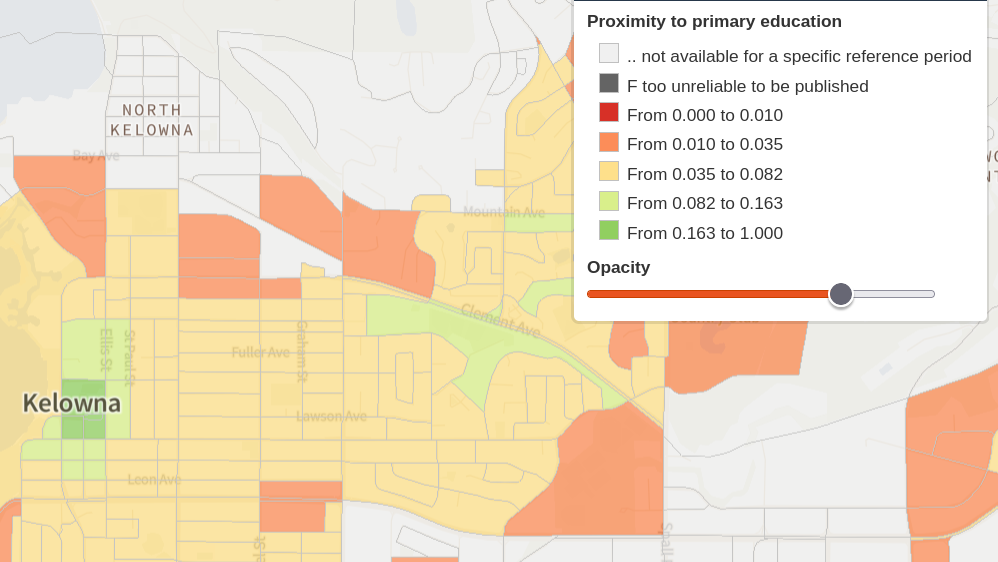
\includegraphics[width=\textwidth]{./PMD_viewer/PMD_viewer.png}
\caption[Proximity Measures Data Viewer]{Statistics Canada’s Proximity Measures Data Viewer showing the proximity to the primary education amenity in Kelowna’s (BC) downtown sector.}\label{pmdviewer}
\end{figure}


A `sister' measure to the PMD is the Index of Remoteness, whose creation is outlined in \textit{Measuring remoteness and accessibility - A set of indices for Canadian communities} by Alasia et. al. A key factor affecting socioeconomic and health outcomes is geographic proximity to population and service centers. As a result, it is an important factor to consider when analyzing and implementing policies and programmes. Statistics Canada developed an Index of Remoteness of communities to measure this factor. The distance to all the population centers (defined by Statistics Canada as areas with a population of at least 1000 and no fewer than 400 person per square kilometers) in a given travel radius, as well as their population size, are taken into account when calculating the index for each populated community (census subdivisions) (Government of Canada, Statistics Canada, 2023). This index was generated as a continuous measure, which was then cut into categories, as outlined in \textit{Developing Meaningful Categories for Distinguishing Levels of Remoteness in Canada} by Subedi et. al. They present five approaches to categorize the continuous measure, which included methods like Jenks natural breaks, k-means, and quintile classification. They aimed to examine various ways to group the continuous remoteness index values of Canadian CSDs into meaningful categories (Government of Canada, Statistics Canada et al., 2020b, August 11). This is similar to our goal of categorizing the continuous proximity measures of amenities.  
\par
The Jenks natural breaks classification and k-means classification techniques are examples of distribution based and centroid based techniques, respectively. Another type of clustering techniques that may be appropriate for our project are density based methods (Geospatial Analysis 6th Edition, 2021 Update - De Smith, Goodchild, Longley and Colleagues, 2021). As Kassambara, a Bioinformatics R\&D Scientist at Veracytes, outlines in his self-published book, the selection of an appropriate clustering technique depends on the nature of the data under investigation. He explains how before applying clustering techniques, it is crucial to assess the clustering tendency to ensure meaningful results, as clustering algorithms may identify clusters even in cases where no clear clusters exist in the data. Additionally, determining the optimal number of clusters is a vital step in the process. Once clustering techniques have been applied, it is important to evaluate their performance using cluster validation statistics such as the silhouette coefficient, Dunn index, and Xie-Beni index. These metrics assist in identifying the most suitable clustering technique for the given data. By considering these factors, researchers can make informed decisions and select the appropriate clustering methodology for specific analysis (Kassambara, 2017b).







\pagebreak 
%%%%%%%%%%%%%%%%%%%%%%%%%%%%%%%%%%%%%%%%
\section{Data}
%%%%%%%%%%%%%%%%%%%%%%%%%%%%%%%%%%%%%%%%




\subsection{Primary Dataset}

The primary dataset of interest for this study is the Proximity Measure Database (PMD), available online and provided by the DEIL at Statistics Canada. The PMD contains continuous numerical proximity measures for 10 amenities, namely: employment, grocery stores, pharmacies, health care, child care, primary education, secondary education, public transit, neighborhood parks, and libraries, for every dissemination block (DB) in Canada within a select radius.
\par
The proximity measures are based on a gravity model that accounts for the distance between a reference DB and all the DBs within a given distance in which the service is available. The proximity measures also take into account the size of services, and the presence of services in the reference DB. The proximity measures are released as a normalized index value, meaning that the values resulting from computations were converted to a scale from 0 to 1, where 0 indicates the lowest proximity, and 1 indicates the highest proximity. When considering a maximum travel radius, the proximity level can be seen as the quantity of service relative to the distance traveled (Alasia et al., 2021). These measures are considered a reliable way to assess local access to various amenities (OECD 2018). The data dictionary for this dataset can be found in Figure~\ref{datadictionary} of the appendix.







\subsection{Missing Values}


Statistics Canada uses a specific convention for representing different types of missing values. Table~\ref{missingvalues} shows the standard symbols that are used by Statistics Canada. The symbols present in the PMD are `..' and `F'.





\begin{table}[H]
\centering
\caption[Missing value symbols]{Missing value symbol convention from Statistics Canada.}\label{missingvalues}
\begin{tabular}{|l|l|} 
\hline
\textbf{Symbol} & \textbf{Meaning} \\
\hline
. & not available for any reference period \\ 
\hline 
.. & not available for a specific reference period \\ 
\hline 
... & not applicable \\ 
\hline 
F & too unreliable to be published \\ 
\hline 
\end{tabular}
\end{table}




Values ``too unreliable to be published'' are most likely due to missing data in the many data sources used to construct the PMD, like Business Register, or other authoritative open data sources, such as the Linkable Open Data Environment, the Open Database of Educational Facilities and the General Transit Feed Specification.
\par
Data that is `not available' for a DB is the result of that DB being out of scope: while producing the PMD, the authors considered a maximum travel radius for each amenity, as a mean to reduce computational complexity as well as to ``reflect the fact that there is an upper limit to how far a person will likely travel for most services'' (Alasia et. Al, 2021). The authors assigned ``..'' when no amenity was available within a given travel radius for a select DB. As a result, not every DB has proximity values for amenities. 
\par
In summary, data points may be unavailable either because the supporting databases are incomplete, or because there is no access to the amenity within the specified travel radius. The fact that a sizable portion of DBs don’t have an associated proximity measure is not a concern for this project, as we want to segment the measures that are within the scope set by the authors of the PMD and we are focused on the clustering methodology rather than the exact summary statistics of the clusters themselves.








\subsection{Other Data}


We linked the Index of Remoteness (IoR) dataset to the PMD to add to the cluster profile analysis. This dataset includes a continuous numeric remoteness score for each census subdivision (CSD) in Canada. The IoR is equal to zero for the least remote CSD and equal to one for the most remote CSD. 









\pagebreak 
%%%%%%%%%%%%%%%%%%%%%%%%%%%%%%%%%%%%%%%%
\section{Methods}
%%%%%%%%%%%%%%%%%%%%%%%%%%%%%%%%%%%%%%%%

We started with an exploratory data analysis to familiarize ourselves with the data and learn its characteristics. We used R and the \texttt{tidyverse} package to handle and analyze the data. Concurrently, we researched clustering algorithms and validation metrics. We moved on to evaluating clustering tendencies of each amenity to assess the natural susceptibility of the data to grouping. Then, we applied various algorithms to each amenity as well as investigated `intuitive' categorizing methods, such as `quintiles' and identifying minima. For each of these methods, computational restraints prevented clustering analyses on the entire dataset. Instead, 3\% subsampling was used to ensure that the algorithms would run successfully and within a reasonable timeframe. We then validated the clusters using the \texttt{ClusterCrit} package. We profiled the resulting clusters for each technique to evaluate the results and their robustness, as well as to gain insights into the characteristics of each cluster. Finally, we made conclusions and recommendations on future work.







\subsection{Data Exploration}


In order to better understand the structure of the data, we performed an exploratory data analysis (EDA). We analyzed numerical variables (all ten amenities plus DB population) in the PMD using summary statistics, and we counted unique values for categorical variables. We also visualized the distributions of each of the ten amenities using density plots, both before and after a log-transformation (an epsilon value of 0.0001 was added prior to log-transforming in order to avoid infinite values). Finally, we identified outliers via boxplots, validated them using Rosner's test, and counted them before and after log-transformation.  





\subsection{Clustering Tendency}


We evaluated the clustering tendency of each amenity via Visual Assessment of Tendency (VAT) as well as sort plots. VAT works by plotting the distance matrix between all observations in the dataset. Sort plots highlight natural breaks in a continuous vector by sorting the values and then plotting them by index. We used \texttt{fviz\_dist} function from the \texttt{factoextra} package to produce the VAT plots. 





\subsection{Quintiles}


The quintile method is the current method employed by Statistics Canada to segment the proximity measures in their data viewer. In this method, data are sorted, and then split into 5 groups, each with the same number of observations. This approach is therefore ``blind'' to the data, since the actual values are not used in the creation of clusters. We considered this approach as the “base model” to which comparisons will be made. 







\subsection{Minima Identification}


This segmentation technique functions by cutting the distribution at select minima of the density distribution. Each minima in the density curves that are flanked by maxima of higher density represent a density sparse region, which may be a `natural' break in the continuous measures. We conducted this non-parametric approach mathematically on the logged transformed data where minima are perceptible. 







\subsection{Clustering}


We explored various clustering techniques, including HDBSCAN, MixAll, K-PAM, VarSelLCM, and OPTICS, to determine possible cutoff values for the amenity proximity measures. We found that only the results from the HDBSCAN, MixAll, Mclust, and PAM k-means algorithms were appropriate. Summaries of the unsuccessful approaches can be found in section~\ref{appendix:successful} of the Appendix.





\subsubsection{Number of Clusters}

In many clustering techniques, the user is typically required to specify the desired number of clusters (k) to be generated (Kassambara, 2017b). To determine the appropriate number of clusters for each clustering technique, various metrics were employed, including the silhouette coefficient, Dunn index, Calinski-Harabasz, and Davies-Bouldin. The number of clusters recommended by the majority of these metrics was ultimately selected and implemented for the specific clustering technique being used. 
\par
Figure~\ref{numselect} is an example of a set of internal evaluation schemes values per number of clusters for the MixAll clustering technique applied on the Employment proximity values. The number of clusters suggested by each metric is as follows:
\begin{itemize}
\item Silhouette coefficient: 2 clusters
\item Dunn index: 3 clusters
\item Calinski-Harabasz: 8 clusters
\item Davies-Bouldin: 8 clusters
\end{itemize}
To determine the final number of clusters, the majority recommendation from these metrics was considered. As 8 clusters were suggested by the majority of the metrics, this number was chosen.



\begin{figure}[H]
\centering
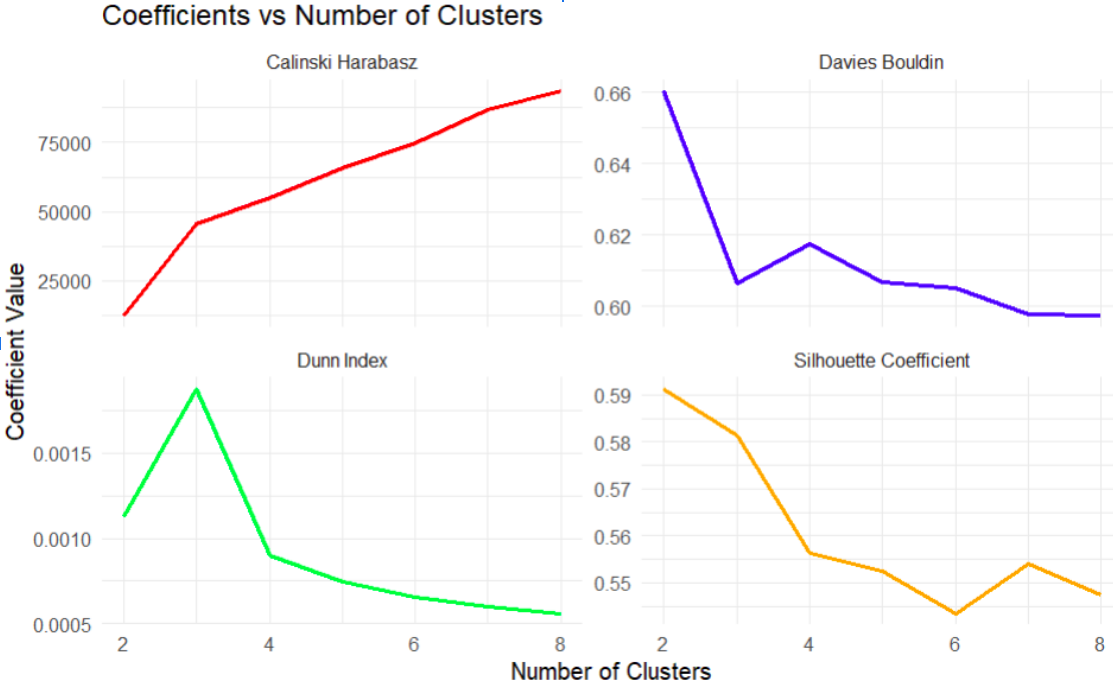
\includegraphics[width=\textwidth]{./coefs_demo/coefs_demo.png}
\caption[Number of cluster selection]{Number of clusters suggested by different metrics for employment amenity in MixAll clustering algorithm. We want to maximize all the metrics except for the Davies-Bouldin, which we want to minimize.}\label{numselect}
\end{figure}






\subsubsection{Comparison of Algorithms}


Due to the conflicting recommendations from clustering validation metrics, such as silhouette coefficients, Dunn index, Calinski-Harabasz, and Davies-Bouldin, it became challenging to select a single clustering technique for profiling purposes. In light of this challenge, a different approach was adopted.
\par
Instead of relying on a single algorithm for cluster profiling, multiple techniques that had proven effective in the univariate case and produced satisfactory results were utilized. This approach allowed for a more comprehensive exploration of the data and ensured that the clustering results were robust, and not solely dependent on a single technique.
\par
The success of several algorithms may also be compared intuitively by looking at how the cutoff values divide the log-transformed density plots for each amenity. Successful algorithms will find the cutoff values to be near the “troughs” or ``density sparse regions'' in these density plots, with the clusters themselves being the ``peaks'' or ``dense regions''. Conversely, poorly performing algorithms will miss these troughs by placing the cutoffs randomly or near the peaks. 





\subsubsection{Cluster Profiles}


Following the identification of clusters, an investigation was conducted to examine the profiles of these clusters. This involved comparing various factors, including the number of DBs, median DB population, median IOR, the mode of Census Metropolitan Area type, top province, mode of amenity density, median proximity measure of the clustered amenity, and the corresponding cutoff values.





















\pagebreak 
%%%%%%%%%%%%%%%%%%%%%%%%%%%%%%%%%%%%%%%%
\section{Results}
%%%%%%%%%%%%%%%%%%%%%%%%%%%%%%%%%%%%%%%%




\subsection{Data Exploration}

\subsubsection{Summary Statistics}

The PMD contains 489,676 rows, each of which corresponds to a unique DB. Each row contains information about DB population, the encompassing CSD and province, an indicator of amenity density, whether or not the DB is within a census metropolitan area (CMA), plus all of the ten proximity measures. The amenity dense indicator is split into low, medium and high density, with around 5,000 getting an `F' for ``too unreliable to be published''. CMA type is divided into four groups: a CMA, not a CMA, a tracted census agglomeration (CA), or an untracted CA (`tracted' in this case refers to whether or not the CA has been subdivided into smaller sections for census purposes). In addition, there is an indicator for each of the ten amenities that relates whether or not the amenity in question resides in the same DB for which the proximity is being calculated. Lastly, there is an indicator for whether or not a DB is considered ``amenity dense.'' 
\par
We've outlined earlier reasons for which DBs may not have proximity measures. Table~\ref{missingdata} shows the amount of DBs that have proximity values for each amenity: Employment has the greatest coverage, at 86.5\%, whereas Library has the least at 23\%. This may be a result of the set travel radius for Employment being much larger, as it covers 10 driving kilometers, whereas libraries are only searched within 1.5 walking kilometers.




% latex table generated in R 3.6.3 by xtable 1.8-4 package
% Tue May 30 13:11:59 2023
\begin{table}[ht]
\centering
\caption[Missing data]{Counts and percentages of missing values of numerical variables in the PMD.}\label{missingdata}
\begin{tabular}{|rcc|}
  \hline
 & DBs with Data Available & Percentage \\ 
  \hline
Employment & 423,602 & 86.5 \\ 
  Pharmacy & 178,521 & 36.5 \\ 
  Childcare & 243,964 & 49.8 \\ 
  Healthcare & 300,465 & 61.4 \\ 
  Grocery & 141,063 & 28.8 \\ 
  Pri. Educ. & 225,359 & 46.0 \\ 
  Sec. Educ. & 141,213 & 28.8 \\ 
  Library & 112,655 & 23.0 \\ 
  Parks & 234,068 & 47.8 \\ 
  Transit & 181,305 & 37.0 \\ 
  DB Pop. & 487,526 & 99.6 \\ 
   \hline
\end{tabular}
\end{table}






Table~\ref{summary} shows the summary statistics for the numerical variables in the PMD, while Table~\ref{categorical} shows the counts for each type of the categorical variables. We see that the 90th percentile of the proximity measures for all amenities are values that are much nearer the smaller end of the domain; the largest value is in Primary Education, at 0.233. This is not the only indicator that this measure is unbalanced: the skew and kurtosis values are all relatively high. 




% latex table generated in R 3.6.3 by xtable 1.8-4 package
% Sat Jun 10 08:13:30 2023
\begin{table}[ht]
\centering
\caption[Summary table]{Summary statistics of numerical variables in the PMD.}\label{summary}
\resizebox{\textwidth}{!}{\begin{tabular}{|r|lllllllllll|}
  \hline
 & Employment & Pharmacy & Childcare & Healthcare & Grocery & Pri. Educ. & Sec. Educ. & Library & Parks & Transit & DB Pop. \\ 
  \hline
1 Dec. & 1e-04 & 0.0075 & 0.0079 & 2e-04 & 0.0144 & 0.0319 & 0.0374 & 0.0508 & 0.0127 & 0.0011 & 0 \\ 
  2 Dec. & 4e-04 & 0.0098 & 0.0152 & 7e-04 & 0.0221 & 0.0416 & 0.0421 & 0.0558 & 0.0203 & 0.0026 & 0 \\ 
  3 Dec. & 0.0013 & 0.0146 & 0.0241 & 0.0018 & 0.0289 & 0.0582 & 0.0485 & 0.0624 & 0.0278 & 0.0045 & 5 \\ 
  4 Dec. & 0.003 & 0.0193 & 0.0348 & 0.0032 & 0.0348 & 0.072 & 0.0586 & 0.0707 & 0.0372 & 0.0067 & 16 \\ 
  5 Dec. & 0.0065 & 0.0256 & 0.0476 & 0.005 & 0.0434 & 0.09 & 0.0745 & 0.0814 & 0.0481 & 0.0094 & 29 \\ 
  6 Dec. & 0.0127 & 0.0341 & 0.0636 & 0.0074 & 0.0555 & 0.1105 & 0.091 & 0.096 & 0.0614 & 0.0131 & 45 \\ 
  7 Dec. & 0.0217 & 0.0457 & 0.0846 & 0.0111 & 0.0719 & 0.1366 & 0.1141 & 0.1168 & 0.0793 & 0.0184 & 66 \\ 
  8 Dec. & 0.0368 & 0.0641 & 0.1167 & 0.0184 & 0.0985 & 0.172 & 0.1492 & 0.1488 & 0.105 & 0.0272 & 100 \\ 
  9 Dec. & 0.0726 & 0.0983 & 0.1751 & 0.0343 & 0.154 & 0.233 & 0.2128 & 0.2106 & 0.1494 & 0.0442 & 173 \\ 
  Min. & 0 & 0 & 0 & 0 & 1e-04 & 4e-04 & 5e-04 & 1e-04 & 0 & 0 & 0 \\ 
  Median & 0.0065 & 0.0256 & 0.0476 & 0.005 & 0.0434 & 0.09 & 0.0745 & 0.0814 & 0.0481 & 0.0094 & 29 \\ 
  Mean & 0.02541 & 0.04438 & 0.07584 & 0.01372 & 0.06991 & 0.11617 & 0.104 & 0.11462 & 0.0692 & 0.01805 & 72 \\ 
  Max. & 1 & 1 & 1 & 1 & 1 & 1 & 1 & 1 & 1 & 1 & 7607 \\ 
  Std. Dev. & 0.0491 & 0.0579 & 0.0874 & 0.0279 & 0.0783 & 0.0917 & 0.0869 & 0.0978 & 0.0685 & 0.027 & 146 \\ 
  Skew & 4.656 & 4.555 & 2.807 & 7.041 & 3.201 & 1.963 & 2.462 & 3.439 & 2.824 & 5.692 & 8 \\ 
  Kurtosis & 38.08 & 37.81 & 14.82 & 95.45 & 17.83 & 8.72 & 11.84 & 18.48 & 17.2 & 72.96 & 152 \\ 
   \hline
\end{tabular}}
\end{table}








%%%%%%%%%%%%
\begin{longtable}{|l|c|}
\hline
\textbf{Variable}  & \textbf{Counts}  \\
\hline
{DBs Per Province} &  \\
\indent\indent \textit{Alberta} & 66,749 \\
\indent\indent \textit{British Columbia} & 52,850 \\
\indent\indent \textit{Manitoba} & 30,669 \\
\indent\indent \textit{New Brunswick} & 14,345 \\
\indent\indent \textit{Newfoundland and Labrador} & 8,756 \\
\indent\indent \textit{Northwest Territories} & 1,495 \\
\indent\indent \textit{Nova Scotia} & 15,279 \\
\indent\indent \textit{Nunavut} & 792 \\
\indent\indent \textit{Ontario} & 133,214 \\
\indent\indent \textit{Prince Edward Island} & 3,639 \\
\indent\indent \textit{Quebec} &  106,251 \\
\indent\indent \textit{Saskatchewan} & 54,118 \\
\indent\indent \textit{Yukon} & 1,519 \\
\hline

{CMA Type} &  \\
\indent\indent \textit{CMA (B)} & 206,709 \\
\indent\indent \textit{Untracted CA (D)} & 53,061 \\
\indent\indent \textit{Tracted CA (K)} & 16,992 \\
\indent\indent \textit{Not a CMA or CA} & 212,914 \\
\hline

{Amenity Dense} &  \\
\indent\indent \textit{Low Density (0)} & 442,179 \\
\indent\indent \textit{Medium Density (1)} & 37,303 \\
\indent\indent \textit{High Density (2)} & 4,827 \\
\indent\indent \textit{Too unreliable to publish (F)} & 5,367 \\
\hline

{Suppressed} &  \\
\indent\indent \textit{Not suppressed (0)} & 484,309 \\
\indent\indent \textit{Info. Suppressed (1)} & 5,367 \\
\hline

\caption[Summary of cateogrical variables]{Summary statistics for categorical variables in the PMD.}\label{categorical}
\end{longtable}







\subsubsection{Distributions}

The distributions of the proximity scores for all amenities are heavily right-skewed, with the majority of the values being grouped around zero. These distributions then appear to decay smoothly. The strong right-skew results from a relatively small number of high access outliers, which influences the distribution when the measures are normalized. Figure~\ref{comparedist} shows the comparison of the density distributions before and after log-transformation. Figures~\ref{dendist} and \ref{logdendist} in section \ref{extra} of the Appendix show these same distributions for all ten amenities. We can already see that the log-transformed distributions are better because the distribution of the proximity values are more normally distributed, and density sparse regions are now visible. Box-Cox and Arcsine transformations were also attempted, but did not yield distributions that were as consistently normally-distributed as those that were log-transformed. It is important to note that log-transforming the proximity measures does not change the structure of the data. In other words, a particular DB `A' in the non-log-transformed data with less proximity than another DB `B' will still have less proximity in the log-transformed data. Statistical summary table~\ref{summary} for the log-transformed data can be found in section \ref{extra} of the Appendix as table~\ref{logsummary}. In contrast, the skew and kurtosis values for the logged data are much smaller, which proves that the log-transformation was successful in reducing the extreme right skew of these proximity values.




\begin{figure}[H]
\centering
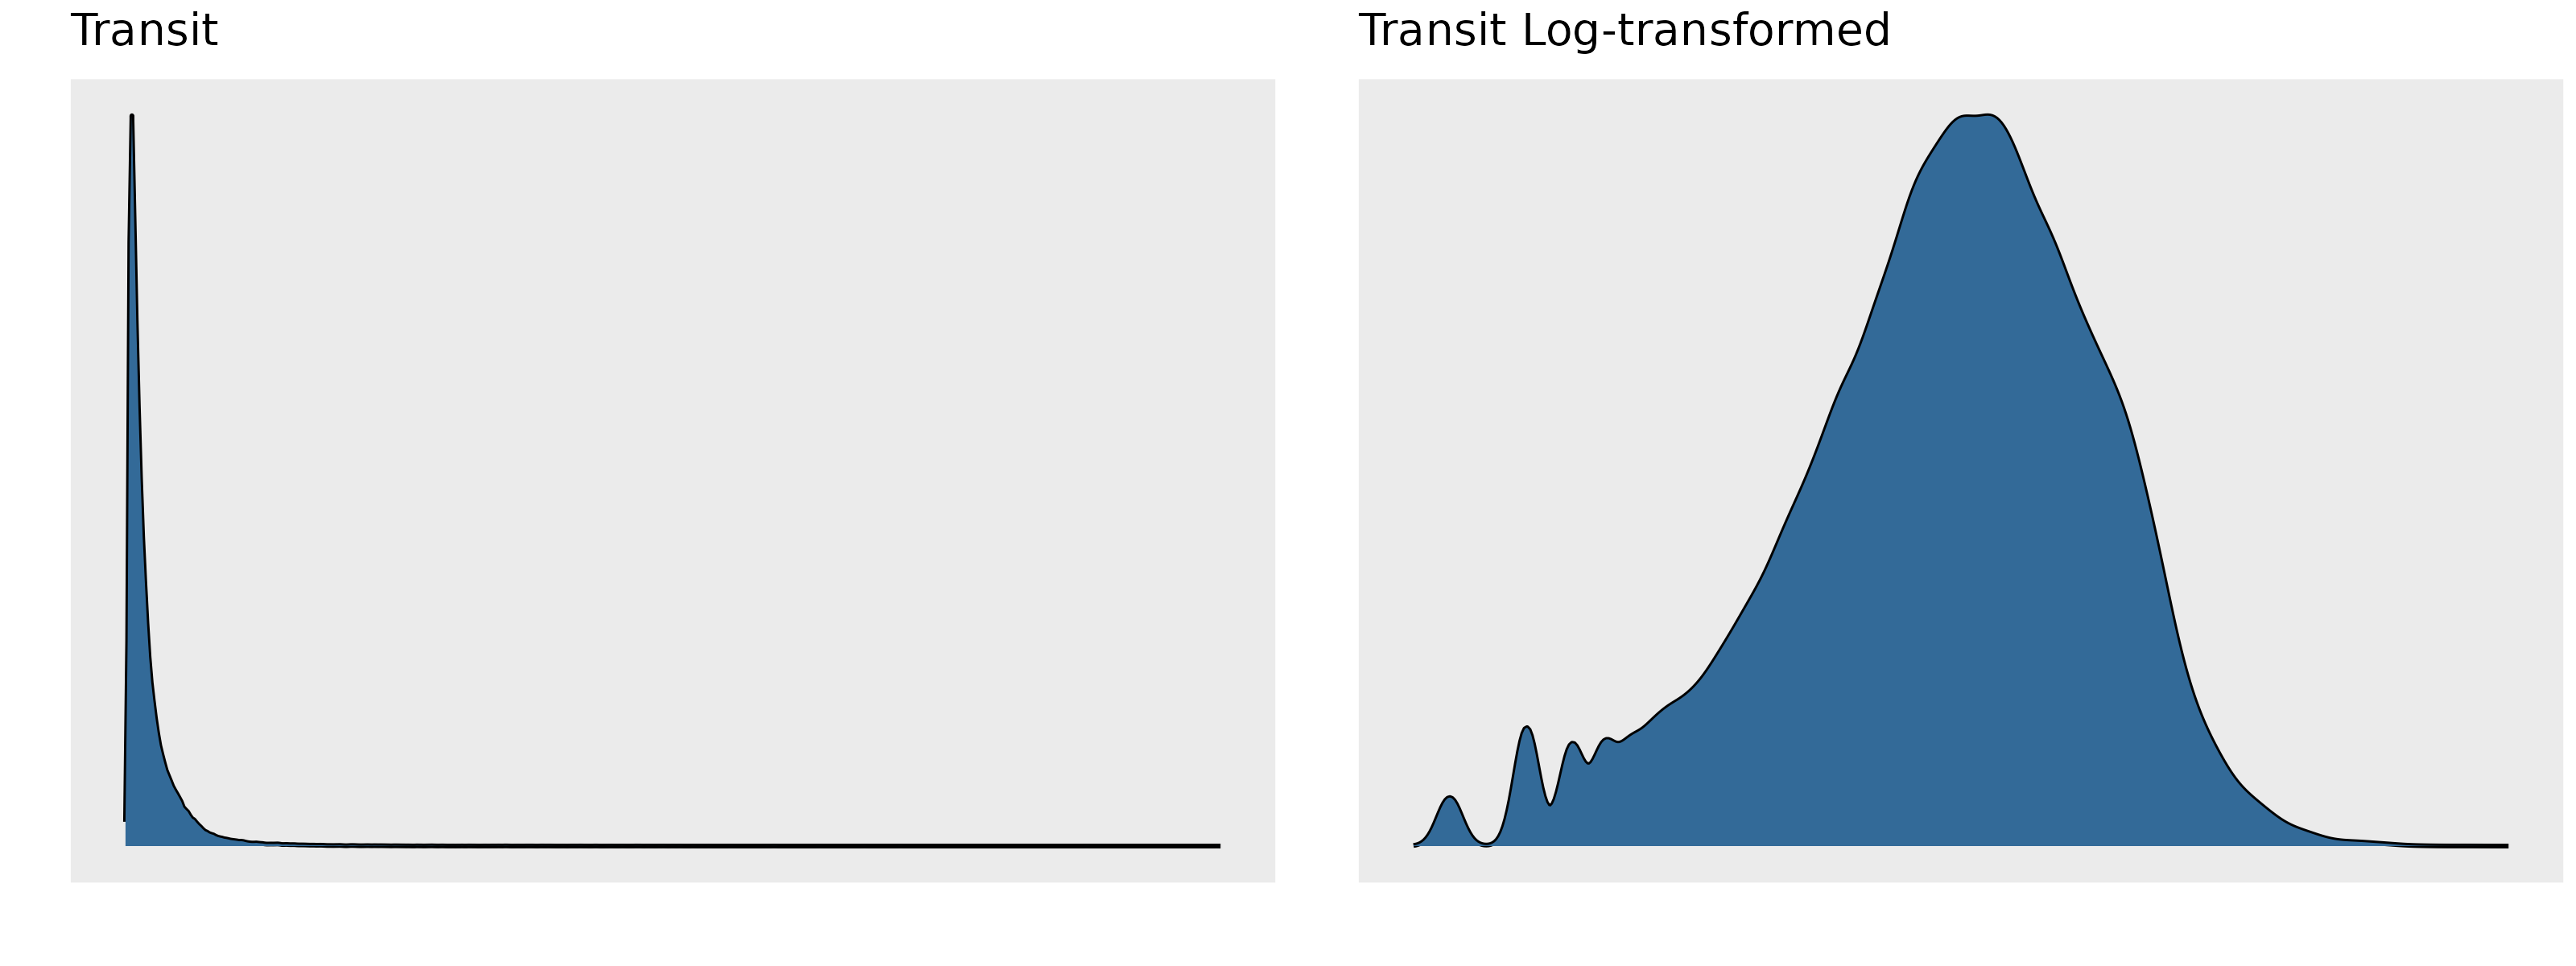
\includegraphics[width=\textwidth]{./distributions/compare_distributions.png}
\caption[Comparison of distributions]{Distribution of the proximity measure to primary education services before and after log-transformation.}\label{comparedist}
\end{figure}



Log-transforming the data is critically important to clustering, and helps reveal the underlying structure. Data points near zero in the non-transformed data are ``clumped'' around particular values, as opposed to being smoothly distributed. This preference for particular values is what creates the miniature peaks that can be seen on the left hand side of the log-transformed density distribution in the employment amenity in Figure~\ref{logdendist} of Appendix section \ref{extra}. These miniature peaks most likely represent real clusters in the data, and are not simply an artifact of the transformation itself. 
\par
Before log-transforming the data, a significant number of outliers were present in the data. Outliers are an issue for most clustering algorithms, since they tend to have a disproportionate impact on the shape of the resulting clusters. The number of outliers was significantly reduced by log-transforming the data, as this reduced the relative distance between points. The reduction in the number of outliers after log-transformation can clearly be seen in table~\ref{outliercounts} (boxplots for visualizing outliers can be found as figures \ref{boxoutliers} and \ref{logboxoutliers} in Appendix section \ref{extra}). In addition to log-transforming the proximity measures to reduce the number of outliers, statistical modeling techniques that are robust to outliers were chosen for clustering.




% latex table generated in R 3.6.3 by xtable 1.8-4 package
% Wed May 31 09:55:20 2023
\begin{table}[h]
\centering
\caption[Number of outliers]{The number of outliers in each amenity in the PMD before and after log-transformation.}\label{outliercounts}
\resizebox{\textwidth}{!}{\begin{tabular}{|r|llll|}
  \hline
 & Counts & Percentages & Log Transformed Counts & Log Transformed Percentages \\ 
  \hline
Employment & 45,390 & 9.27 & 0 & 0.00 \\ 
  Pharmacy & 13,416 & 2.74 & 478 & 0.10 \\ 
  Childcare & 15,397 & 3.14 & 140 & 0.03 \\ 
  Healthcare & 31,007 & 6.33 & 50 & 0.01 \\ 
  Grocery & 11,904 & 2.43 & 794 & 0.16 \\ 
  Pri. Educ. & 10,205 & 2.08 & 98 & 0.02 \\ 
  Sec. Educ. & 8,683 & 1.77 & 215 & 0.04 \\ 
  Library & 8,867 & 1.81 & 2,295 & 0.47 \\ 
  Parks & 12,703 & 2.59 & 910 & 0.19 \\ 
  Transit & 14,165 & 2.89 & 3,596 & 0.73 \\ 
   \hline
\end{tabular}}
\end{table}



\par
Due to the reduction in the number of outliers as well as the improvement in distribution shape (high right skew to quasi-normal), the following clustering analyses were performed on the individual log-transformed measures as opposed to the original measures. For clarity, it is also pertinent to mention that the proximity measures were clustered individually as opposed to being clustered in concert with other variables. This approach was chosen for its simplicity, but other multivariate clustering approaches should be attempted in the future. 










\subsection{Clustering Tendency}


The first of the two assessments of clustering tendency was the VAT. In this test, highly clusterable data is visualized having clearly defined rectangles that lie along the diagonal. In contrast, data with low clustering tendency does not have clear rectangles lying along the diagonal, but instead has a jumble of lines and inconsistent colouring. In the VAT plots for the non-transformed data, consistent low clustering tendency is observed. For the log-transformed data, it seems as though the data is semi-clusterable, as there are rectangles, but they are poorly defined and not as distinct as they could be. The VAT plot for the log-transformed proximity measure of the primary education amenity is shown in Figure~\ref{prieducvat}. The VAT plots for the remaining amenities are available in section~\ref{extra} of the Appendix. 




\begin{figure}[H]
\centering
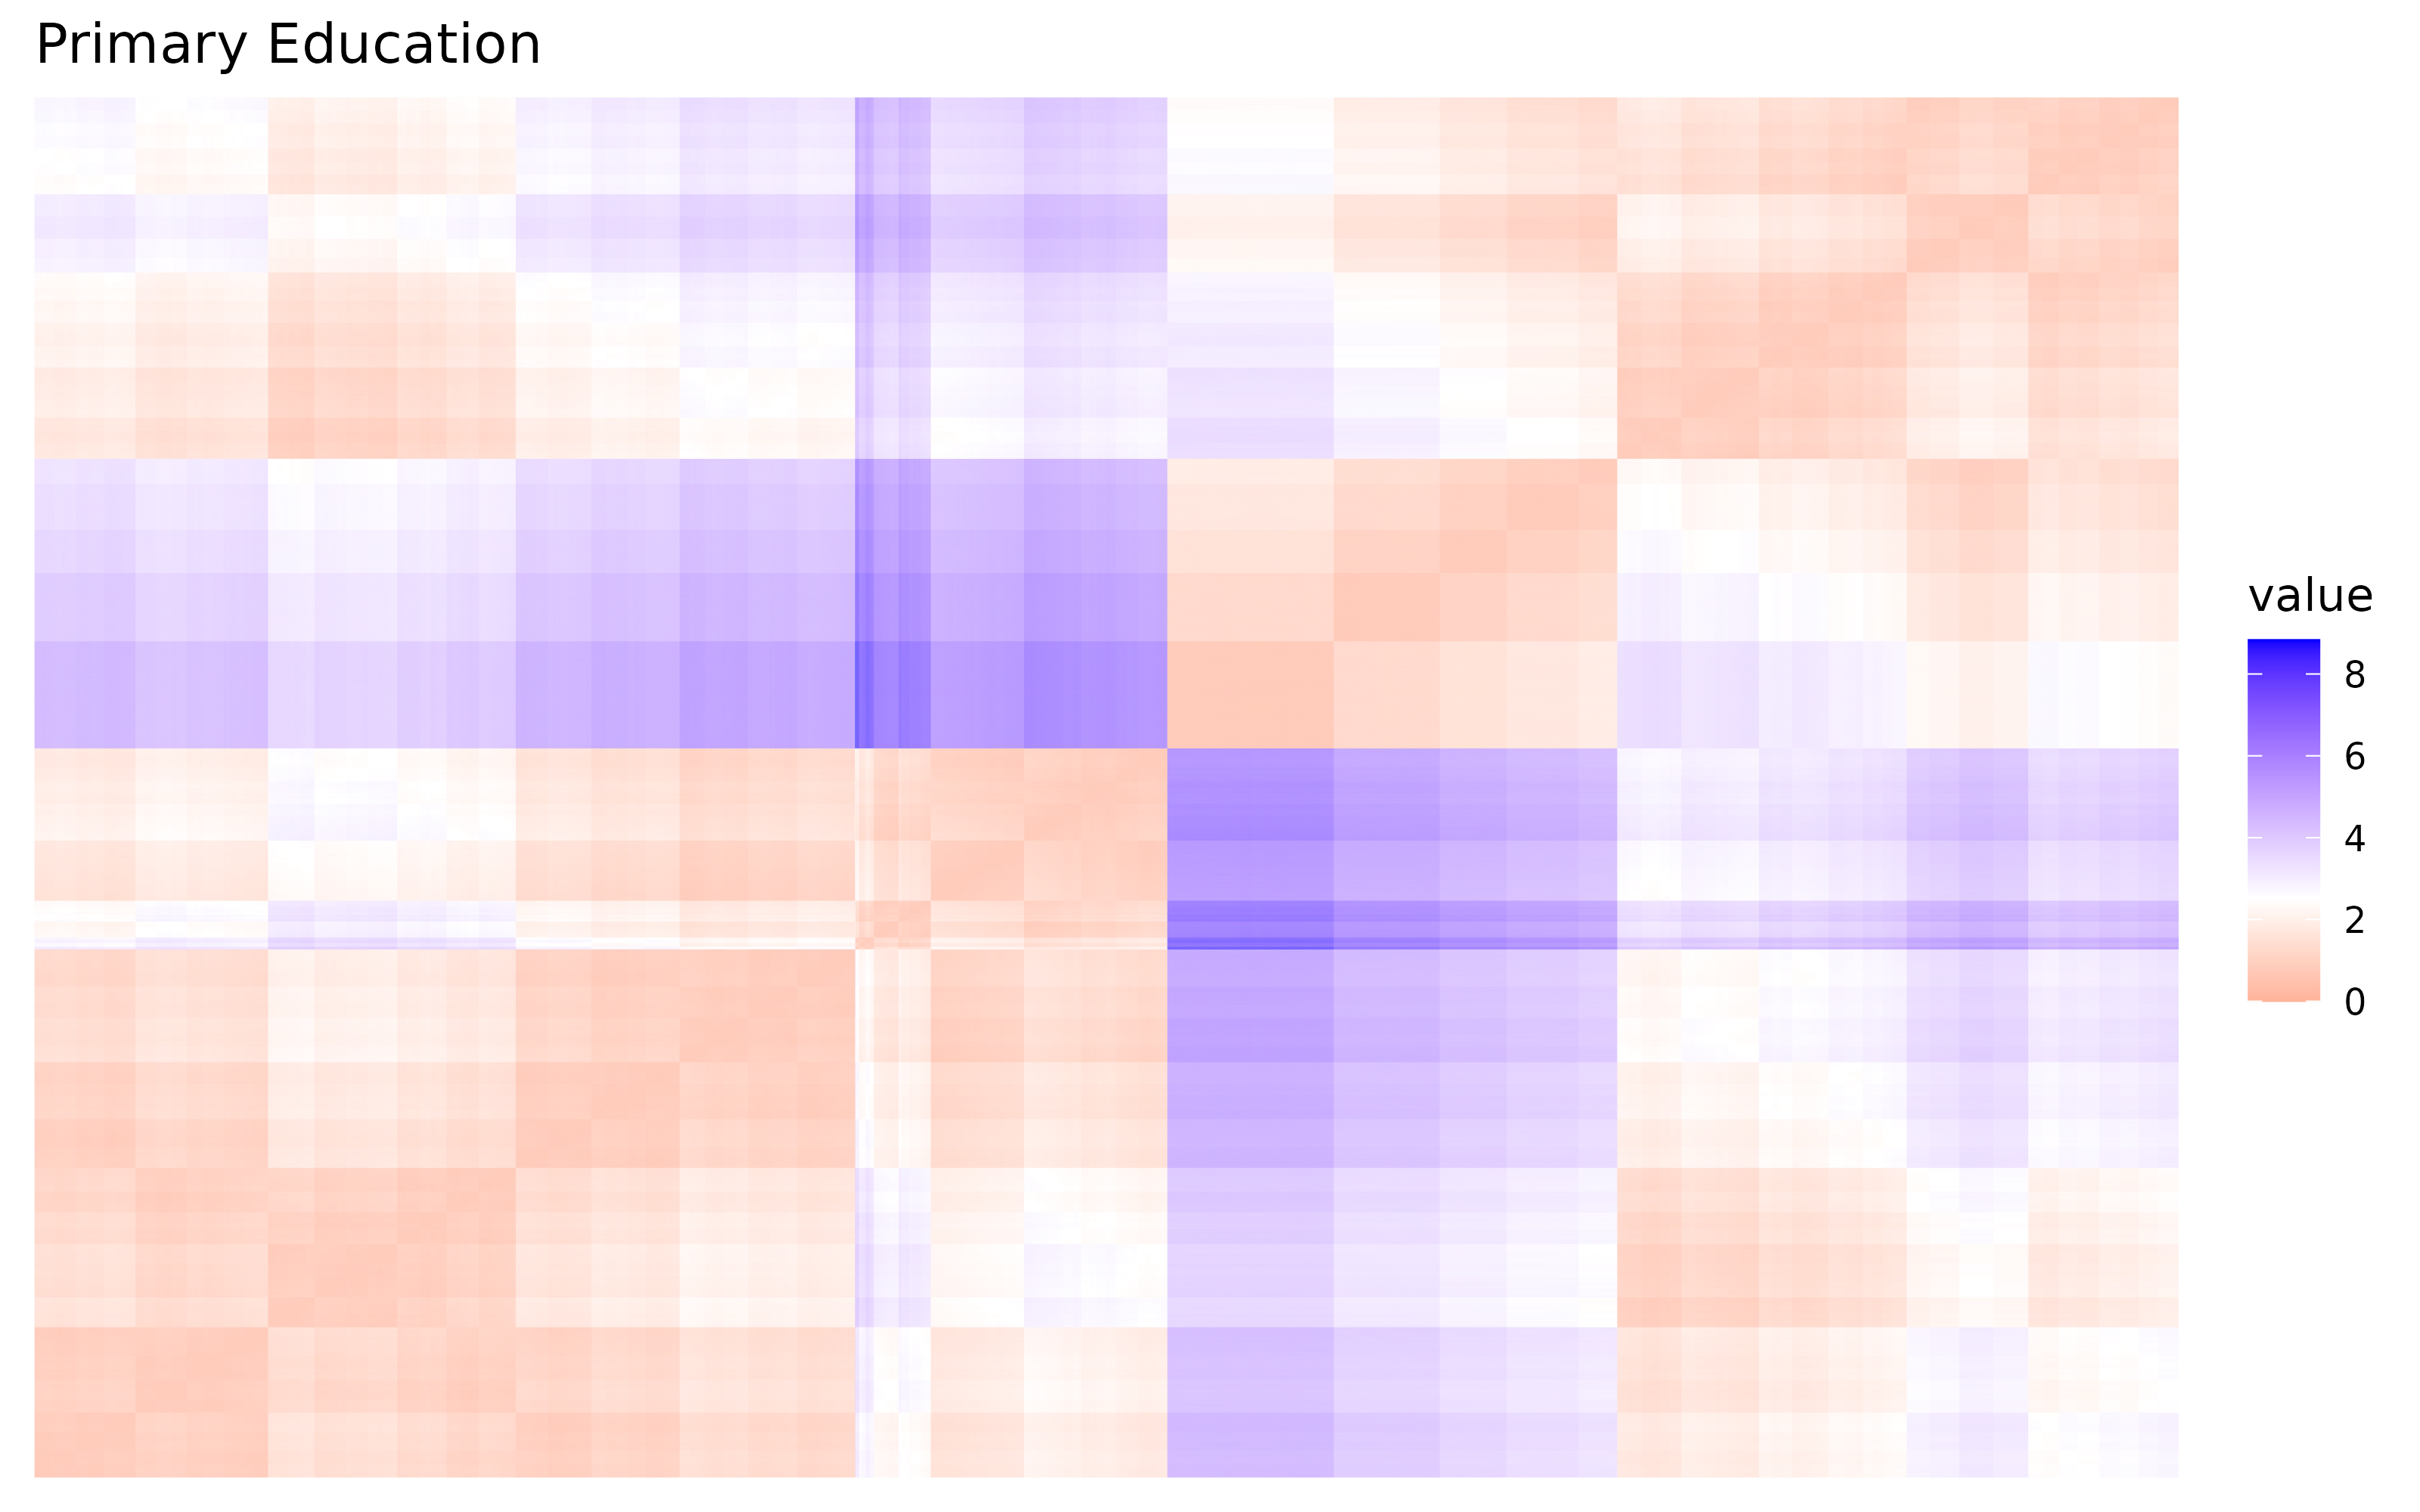
\includegraphics[width=\textwidth]{./vat/primaryeducation_vat_log.png}
\caption[Primary education VAT plot]{VAT plot results for the log-transformed proximity measure of the primary education amenity.}\label{prieducvat}
\end{figure}




The second of the two assessments of clustering tendency was sort plots. If a unidimensional dataset is highly clusterable, then the sort plots will show obvious discontinuous points and changes in slope which separate the clusters. However, this is not observed, as is shown in Figure~\ref{sortplotcompare}. The non-transformed and log-transformed sort plots for the primary education amenity are shown here for an example. Instead of showing obvious breaks, the lines are smooth. This indicates that there are not any obvious clusters in either the non-transformed or log-transformed data. This has implications for the interpretability of our results, as the cutoff points identified between clusters may be sensitive to changes in the data. 






\begin{figure}[H]
\centering
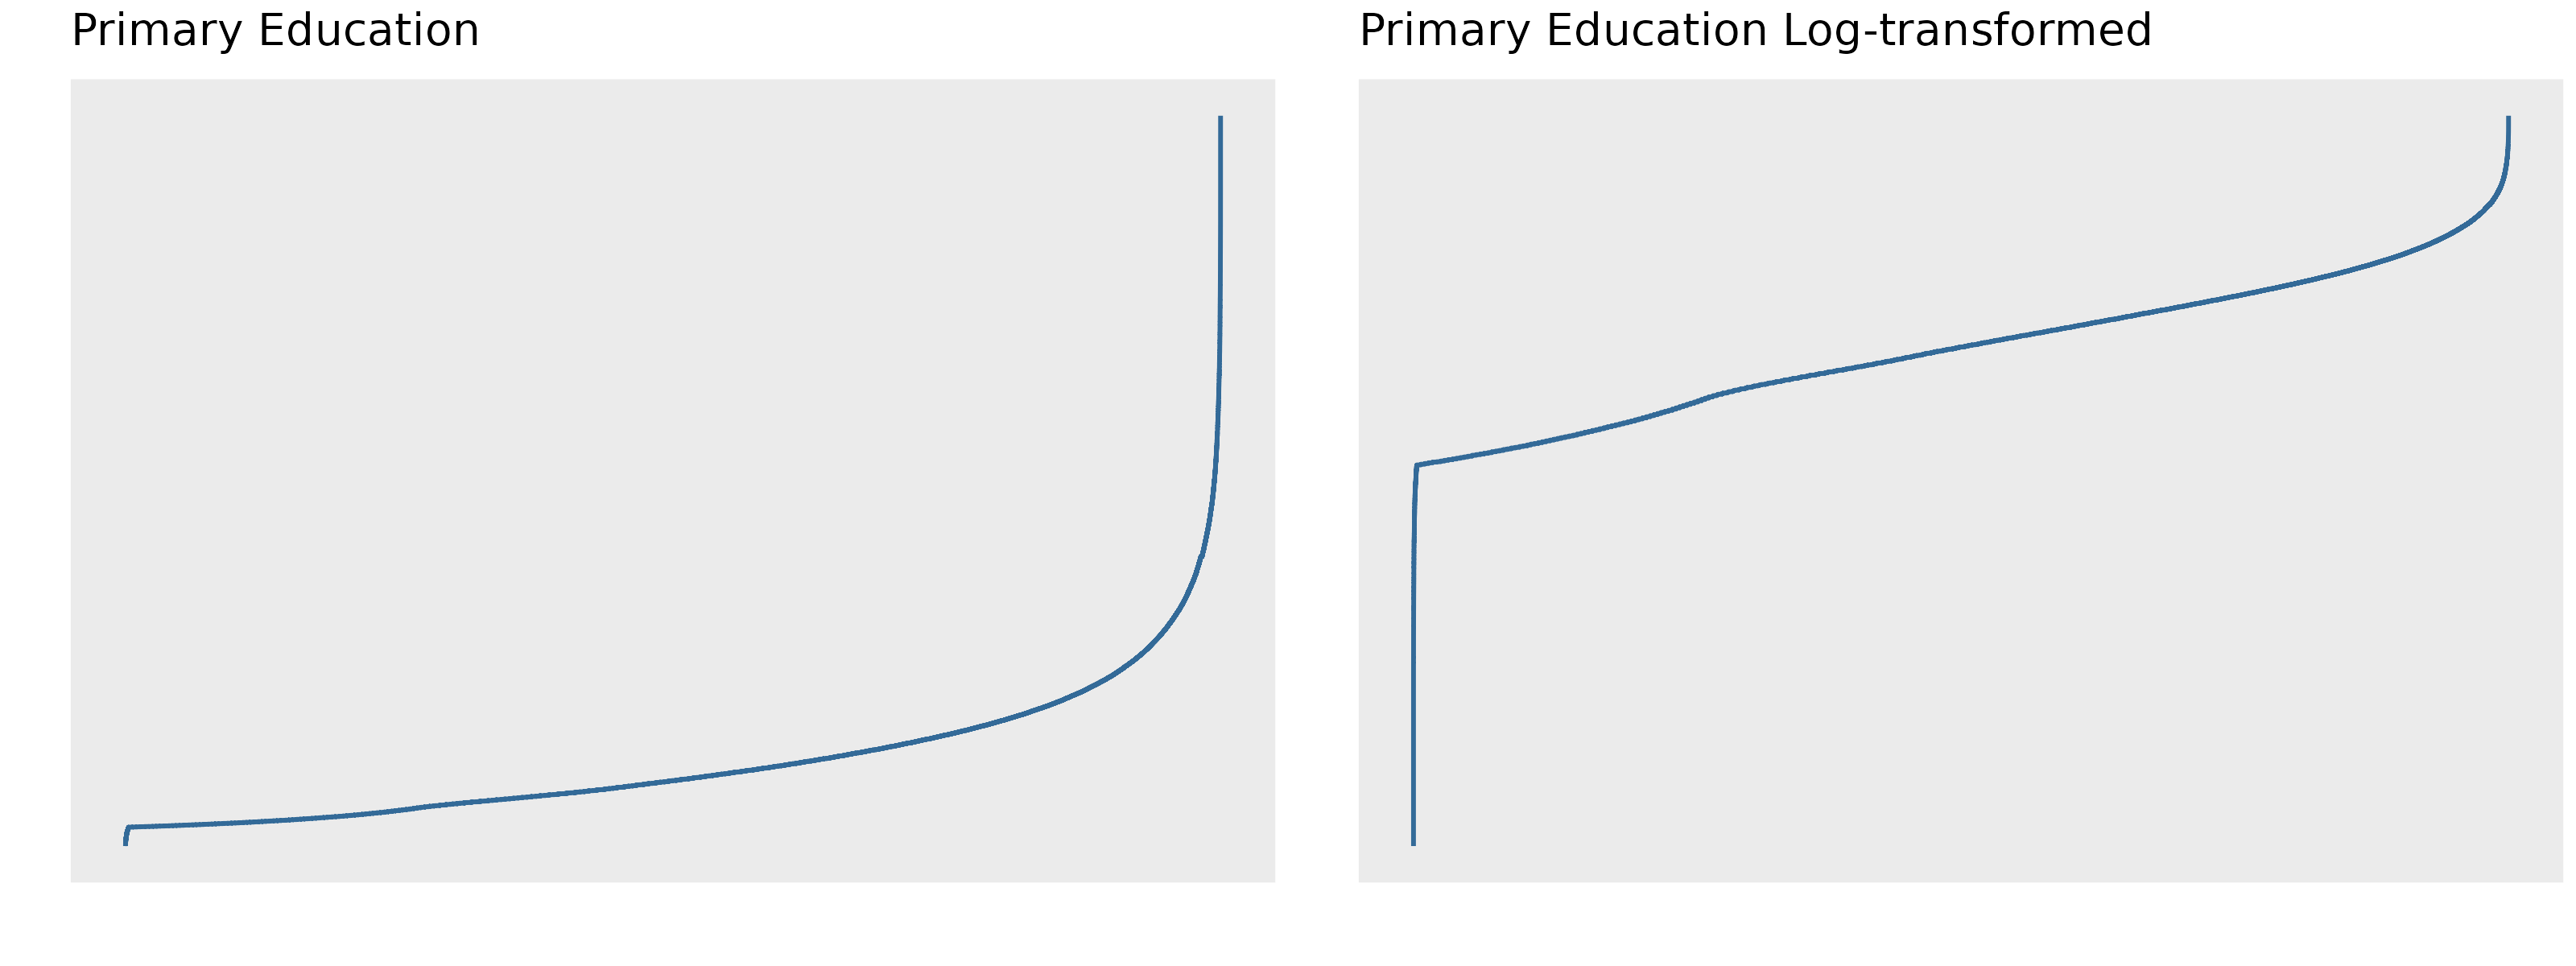
\includegraphics[width=\textwidth]{./sort_plot/sort_comparison.png}
\caption[Primary education sort plot]{Sort plots of the proximity measure to primary education services before and after log-transformation.}\label{sortplotcompare}
\end{figure}








\subsection{Quintiles}

While easy to understand, the quintile method is a ``blind'' algorithm, and therefore fails to find good cutoff values. As seen in figure~\ref{prieduccutoffs}, the cutoffs mostly miss the density sparse regions, and are able to find them only in a few cases by mistake. 






\subsection{Minima Identification}


This method is the most intuitive: the minima of the kernel density curves represent density sparse regions, which may be appropriate areas to segment between naturally occurring groups. However, as seen in Figure~\ref{prieduccutoffs}, for many amenities there are large portions of the curve that do not have mathematical minima, resulting in some groups being much larger than others. If choosing cutoff values fully manually, one may choose a point where the curve plateaus or has a flatter slope. Future work may include mathematically finding points where the second derivative changes signs. 
\par
We used the \texttt{density} function in the \texttt{stats} package with the default bandwidth and the default gaussian kernels to create the density curves. Changing the bandwidth of the kernel density has an effect on the results: smaller bandwidths result in more density sparse regions and more minima, whereas greater bandwidths result in `flatter' curves and less minima. Future work should investigate how the size of the bandwidth affects the resulting clusters. 
\par
There were many unexpected mathematical minima in the density curves in areas where the density was very small and flat. To retain only the minima that represent density sparse regions amongst regions with higher density, a limiting threshold of 0.001 was set for the difference between neighbouring maxima and minima. Intuitively, if the difference between a local maximum and a local minimum was very small, then the minimum is not representative of a good segmentation point. 
\par
Given that the cutoff points selected in this method directly represent density sparse regions, which we intuitively think of as `gaps' between groups, we expect the validation metrics to be better than those for the `quintiles' method. We see that, for example, in the case of the employment amenity, only some of the metrics are better, like the silhouette coefficient and the Dunn index, whilst the Davies-Bouldin and the Calinski-Harabasz actually perform worse. This incongruity is a result of what each of these metrics calculates and represents. 





\subsection{Clustering}

\subsubsection{Comparison of Algorithms}


We have applied many clustering algorithms, the details of which are outlined in section~\ref{appendix:successful} of the Appendix. The univariate algorithms that were successful for our data were: MixAll, HBDSCAN, PAM k-means, and MCLUST. Figure~\ref{prieduccutoffs} shows the plots of the logged-transformed density distributions with the resulting groups coloured for the representative amenity of Primary Education, while Table~\ref{numclusts} outlines specifically the number of groups each method suggested. We can already see how most of the time, the cutoff values for the different methods don’t align with each other: each method finds different points where to segment the data. Even when some methods find more groups than others, aggregating some of the smaller groups doesn't necessarily result in the larger group of another method.  





\begin{figure}[H]
\centering
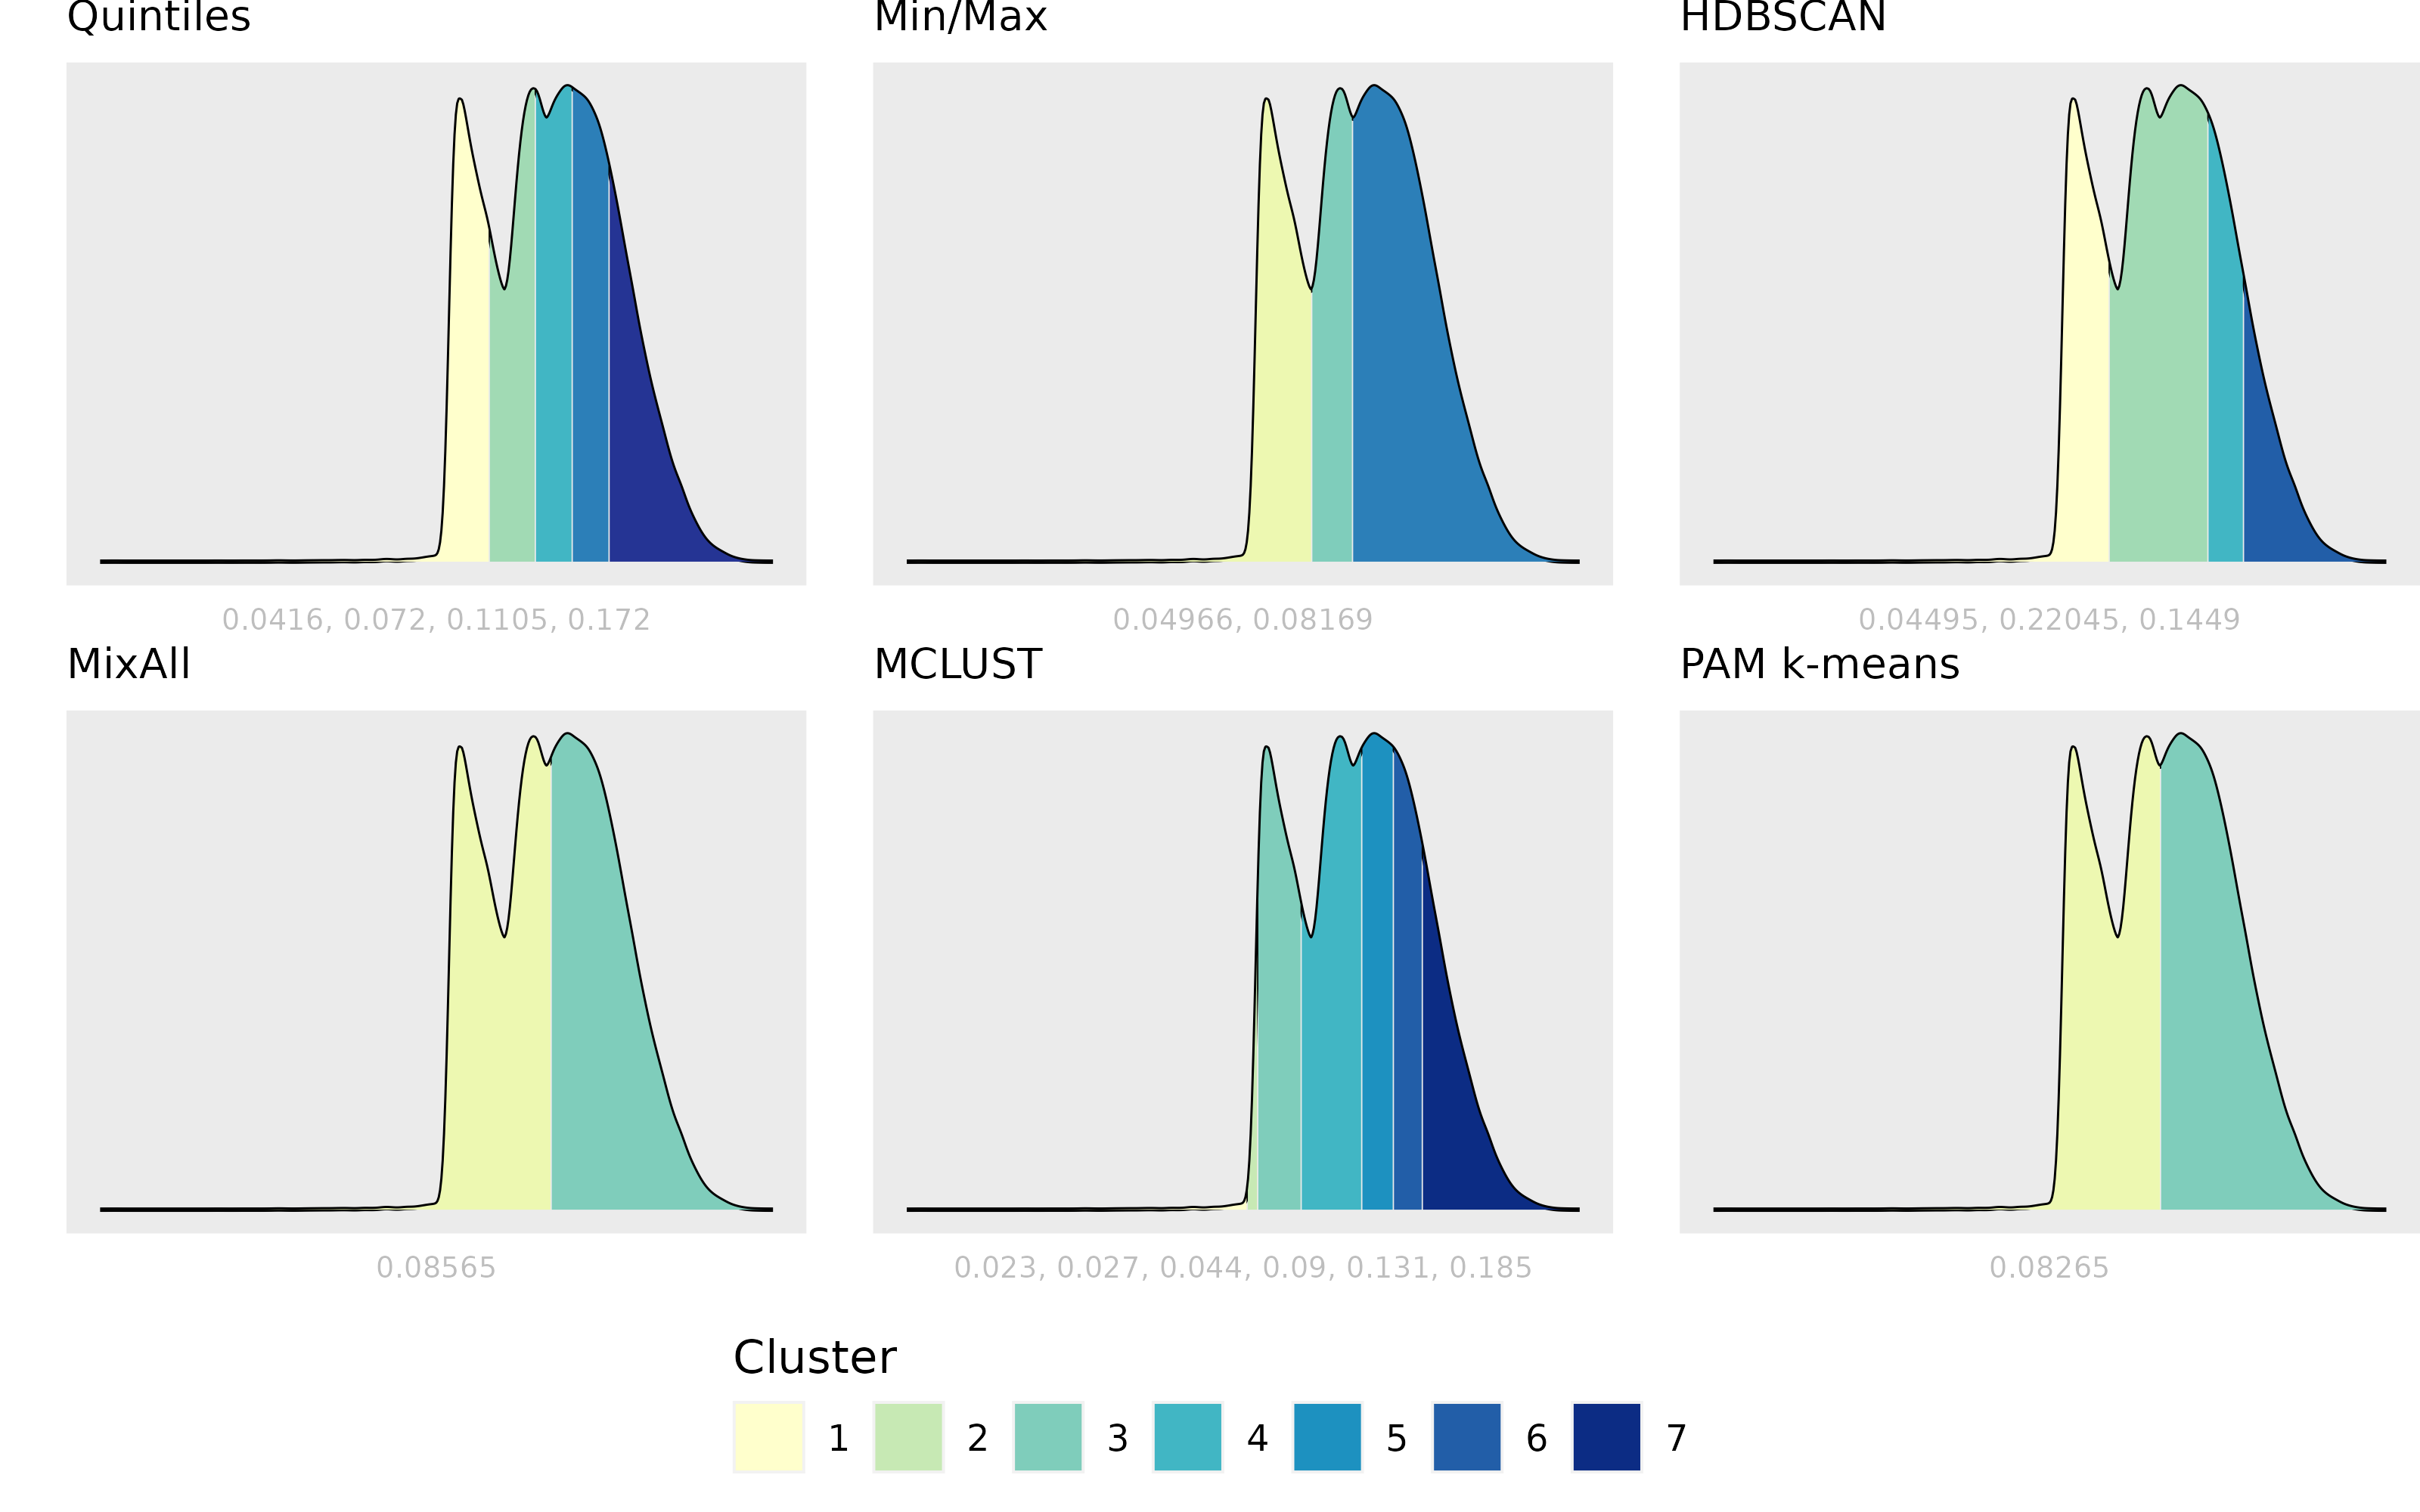
\includegraphics[width=\textwidth]{./cutoffs/by_amenity/Primary Education_cutoffs.png}
\caption[Primary education cutoffs]{Cutoff values from each segmentation approach displayed on the log-transformed density distributions for the primary education amenity.}\label{prieduccutoffs}
\end{figure}









% latex table generated in R 3.6.3 by xtable 1.8-4 package
% Fri Jun  9 12:05:37 2023
\begin{table}[H]
\centering
\caption[Number of clusters by approach]{The number of clusters suggested by all approaches for each amenity in the PMD.}\label{numclusts}
\resizebox{\textwidth}{!}{\begin{tabular}{|r|llllllllll|}
  \hline
 & Emp. & Pharm. & Child. & Health. & Groc. & Pri. Educ. & Sec. Educ. & Lib. & Parks & Transit \\ 
  \hline
Quintiles & 5 & 5 & 5 & 5 & 5 & 5 & 5 & 5 & 5 & 5 \\ 
  Min/Max & 5 & 3 & 3 & 4 & 3 & 3 & 2 & 2 & 3 & 4 \\ 
  HDBSCAN & 2 & 3 & 2 & 2 & 3 & 4 & 3 & 4 & 2 & 2 \\ 
  MixAll & 2 & 2 & 2 & 2 & 2 & 2 & 3 & 2 & 2 & 2 \\ 
  MCLUST & 9 & 7 & 3 & 4 & 3 & 7 & 8 & 7 & 8 & 3 \\ 
  PAM k-means & 2 & 2 & 2 & 2 & 8 & 2 & 4 & 2 & 2 & 2 \\ 
   \hline
\end{tabular}}
\end{table}











%example text Table~\ref{prieducmetrics} ...

% latex table generated in R 3.6.3 by xtable 1.8-4 package
% Fri Jun  9 10:09:08 2023
\begin{longtable}[H]{|r|llll|}
  \hline
 & Silhouette & Dunn & Calinski Harabasz & Davies Bouldin \\ 
  \hline
Quintiles & 0.47 & 0.00000 &  6013 & 0.71 \\ 
   \hline
MixAll & 0.58 & 0.00033 & 15104 & 0.67 \\ 
   \hline
HDBSCAN & 0.33 & 0.00009 &  2594 & 2.69 \\ 
   \hline
PAM k-means & 0.59 & 0.00038 & 15239 & 0.66 \\ 
   \hline
MCLUST & 0.46 & 0.00043 & 18424 & 0.65 \\ 
   \hline
Min/Max & 0.45 & 0.00015 &  2853 & 0.64 \\ 
   \hline
\caption[Primary education validation metrics]{ The validation metric values for each clustering approach for the primary education amenity.}\label{prieducmetrics} 
\end{longtable}












\subsubsection{Cluster Profiles}


Table~\ref{prieducprofile} shows the profiles of each of the clusters defined by each of the successful univariate clustering algorithms for the primary education amenity. The cluster numbers were sorted by cutoff values so that the clusters with the least amenity proximity are \#1, and those with the most proximity are larger numbers. The other summary variables seem to be roughly correlated with proximity to primary education: as this proximity increases, DB population seems to increase, median IoR seems to decrease, percentage of CMA DBs increases, percentage of DBs in Ontario increases, and the percentage of low amenity dense DBs decreases. All of these trends seem to indicate that proximity to primary education is highest in densely populated cities. Figure~\ref{prieducbarplot} summarizes these same clusters by showing the number of DBs and number of people in each cluster for each algorithm. 




\begin{table}[H]
\centering
\resizebox{\textwidth}{!}{\begin{tabular}{|r|llllllll|}
  \hline
 & \# of DBs & DB Population & Median IoR & CMA Type & Province & Amenity Dense & Pri. Educ. & Range \\ 
  \hline
Entire Population & 225,359 (100.0\%) & 61 & 0.12 & CMA (65.6\%) & Ontario (24.3\%) & Low (81.3\%) & 0.090 & 0 - 1 \\ 
  Quintiles C1 & 44,802 (19.9\%) & 47 & 0.15 & CMA (53.4\%) & Ontario (17.4\%) & Low (93.1\%) & 0.032 & 0 - 0.0416 \\ 
  Min/Max C1 & 57,009 (25.3\%) & 47 & 0.15 & CMA (52.6\%) & Ontario (17.1\%) & Low (92.9\%) & 0.034 & 0 - 0.0497 \\ 
  HDBSCAN C1 & 50,263 (22.3\%) & 47 & 0.15 & CMA (53.0\%) & Ontario (17.2\%) & Low (93.0\%) & 0.033 & 0 - 0.0449 \\ 
  MixAll C1 & 107,488 (47.7\%) & 50 & 0.14 & CMA (56.1\%) & Ontario (19.1\%) & Low (90.7\%) & 0.047 & 0 - 0.0857 \\ 
  MCLUST C1 & 518 (0.2\%) & 127 & 0.30 & None (72.6\%) & NovaScotia (10.0\%) & Low (100.0\%) & 0.018 & 0 - 0.0235 \\ 
  PAM k-means C1 & 104,320 (46.3\%) & 50 & 0.14 & CMA (55.8\%) & Ontario (19.0\%) & Low (90.8\%) & 0.046 & 0 - 0.0827 \\ 
  Quintiles C2 & 44,830 (19.9\%) & 51 & 0.14 & CMA (56.1\%) & Ontario (19.3\%) & Low (89.8\%) & 0.058 & 0.0416 - 0.0720 \\ 
  Min/Max C2 & 45,865 (20.4\%) & 53 & 0.14 & CMA (59.7\%) & Ontario (21.2\%) & Low (88.4\%) & 0.066 & 0.0497 - 0.0817 \\ 
  HDBSCAN C2 & 113,383 (50.3\%) & 59 & 0.12 & CMA (64.3\%) & Ontario (24.3\%) & Low (84.9\%) & 0.085 & 0.0449 - 0.1449 \\ 
  MixAll C2 & 117,871 (52.3\%) & 69 & 0.11 & CMA (74.3\%) & Ontario (29.0\%) & Low (72.8\%) & 0.149 & 0.0857 - 1 \\ 
  MCLUST C2 & 1,794 (0.8\%) & 48 & 0.15 & CMA (53.2\%) & Ontario (16.6\%) & Low (93.9\%) & 0.026 & 0.0235 - 0.0265 \\ 
  PAM k-means C2 & 121,039 (53.7\%) & 69 & 0.11 & CMA (74.1\%) & Ontario (28.9\%) & Low (73.1\%) & 0.147 & 0.0827 - 1 \\ 
  Quintiles C3 & 45,503 (20.2\%) & 60 & 0.12 & CMA (65.4\%) & Ontario (24.9\%) & Low (84.6\%) & 0.090 & 0.0720 - 0.1105 \\ 
  Min/Max C3 & 122,485 (54.4\%) & 69 & 0.11 & CMA (73.9\%) & Ontario (28.8\%) & Low (73.3\%) & 0.146 & 0.0817 - 1 \\ 
  HDBSCAN C3 & 35,780 (15.9\%) & 70 & 0.11 & CMA (76.4\%) & Ontario (29.9\%) & Low (71.8\%) & 0.174 & 0.1449 - 0.2204 \\ 
  MCLUST C3 & 47,196 (20.9\%) & 46 & 0.15 & CMA (53.4\%) & Ontario (17.4\%) & Low (92.9\%) & 0.033 & 0.0265 - 0.0444 \\ 
  Quintiles C4 & 45,120 (20.0\%) & 67 & 0.11 & CMA (73.7\%) & Ontario (29.9\%) & Low (77.3\%) & 0.137 & 0.1105 - 0.1720 \\ 
  HDBSCAN C4 & 25,933 (11.5\%) & 82 & 0.09 & CMA (80.7\%) & Ontario (30.0\%) & Low (55.9\%) & 0.285 & 0.2204 - 1 \\ 
  MCLUST C4 & 63,570 (28.2\%) & 54 & 0.14 & CMA (59.1\%) & Ontario (20.9\%) & Low (88.3\%) & 0.067 & 0.0444 - 0.0901 \\ 
  Quintiles C5 & 45,104 (20.0\%) & 77 & 0.10 & CMA (79.3\%) & Ontario (29.9\%) & Low (61.9\%) & 0.233 & 0.1720 - 1 \\ 
  MCLUST C5 & 40,185 (17.8\%) & 64 & 0.11 & CMA (70.0\%) & Ontario (28.0\%) & Low (81.5\%) & 0.109 & 0.0901 - 0.1312 \\ 
  MCLUST C6 & 33,300 (14.8\%) & 69 & 0.11 & CMA (75.0\%) & Ontario (29.8\%) & Low (75.0\%) & 0.154 & 0.1312 - 0.1850 \\ 
  MCLUST C7 & 38,796 (17.2\%) & 78 & 0.10 & CMA (79.9\%) & Ontario (30.0\%) & Low (60.1\%) & 0.247 & 0.1850 - 1 \\ 
   \hline
\end{tabular}}
\caption[Primary education cluster profiles]{Summary statistics for each cluster found by all approaches for the primary education amenity. DB Population, IoR and proximity value show the median, while CMA Type, Province and Amenity Dense show the mode.}\label{prieducprofile}
\end{table}









\begin{figure}[H]
\centering
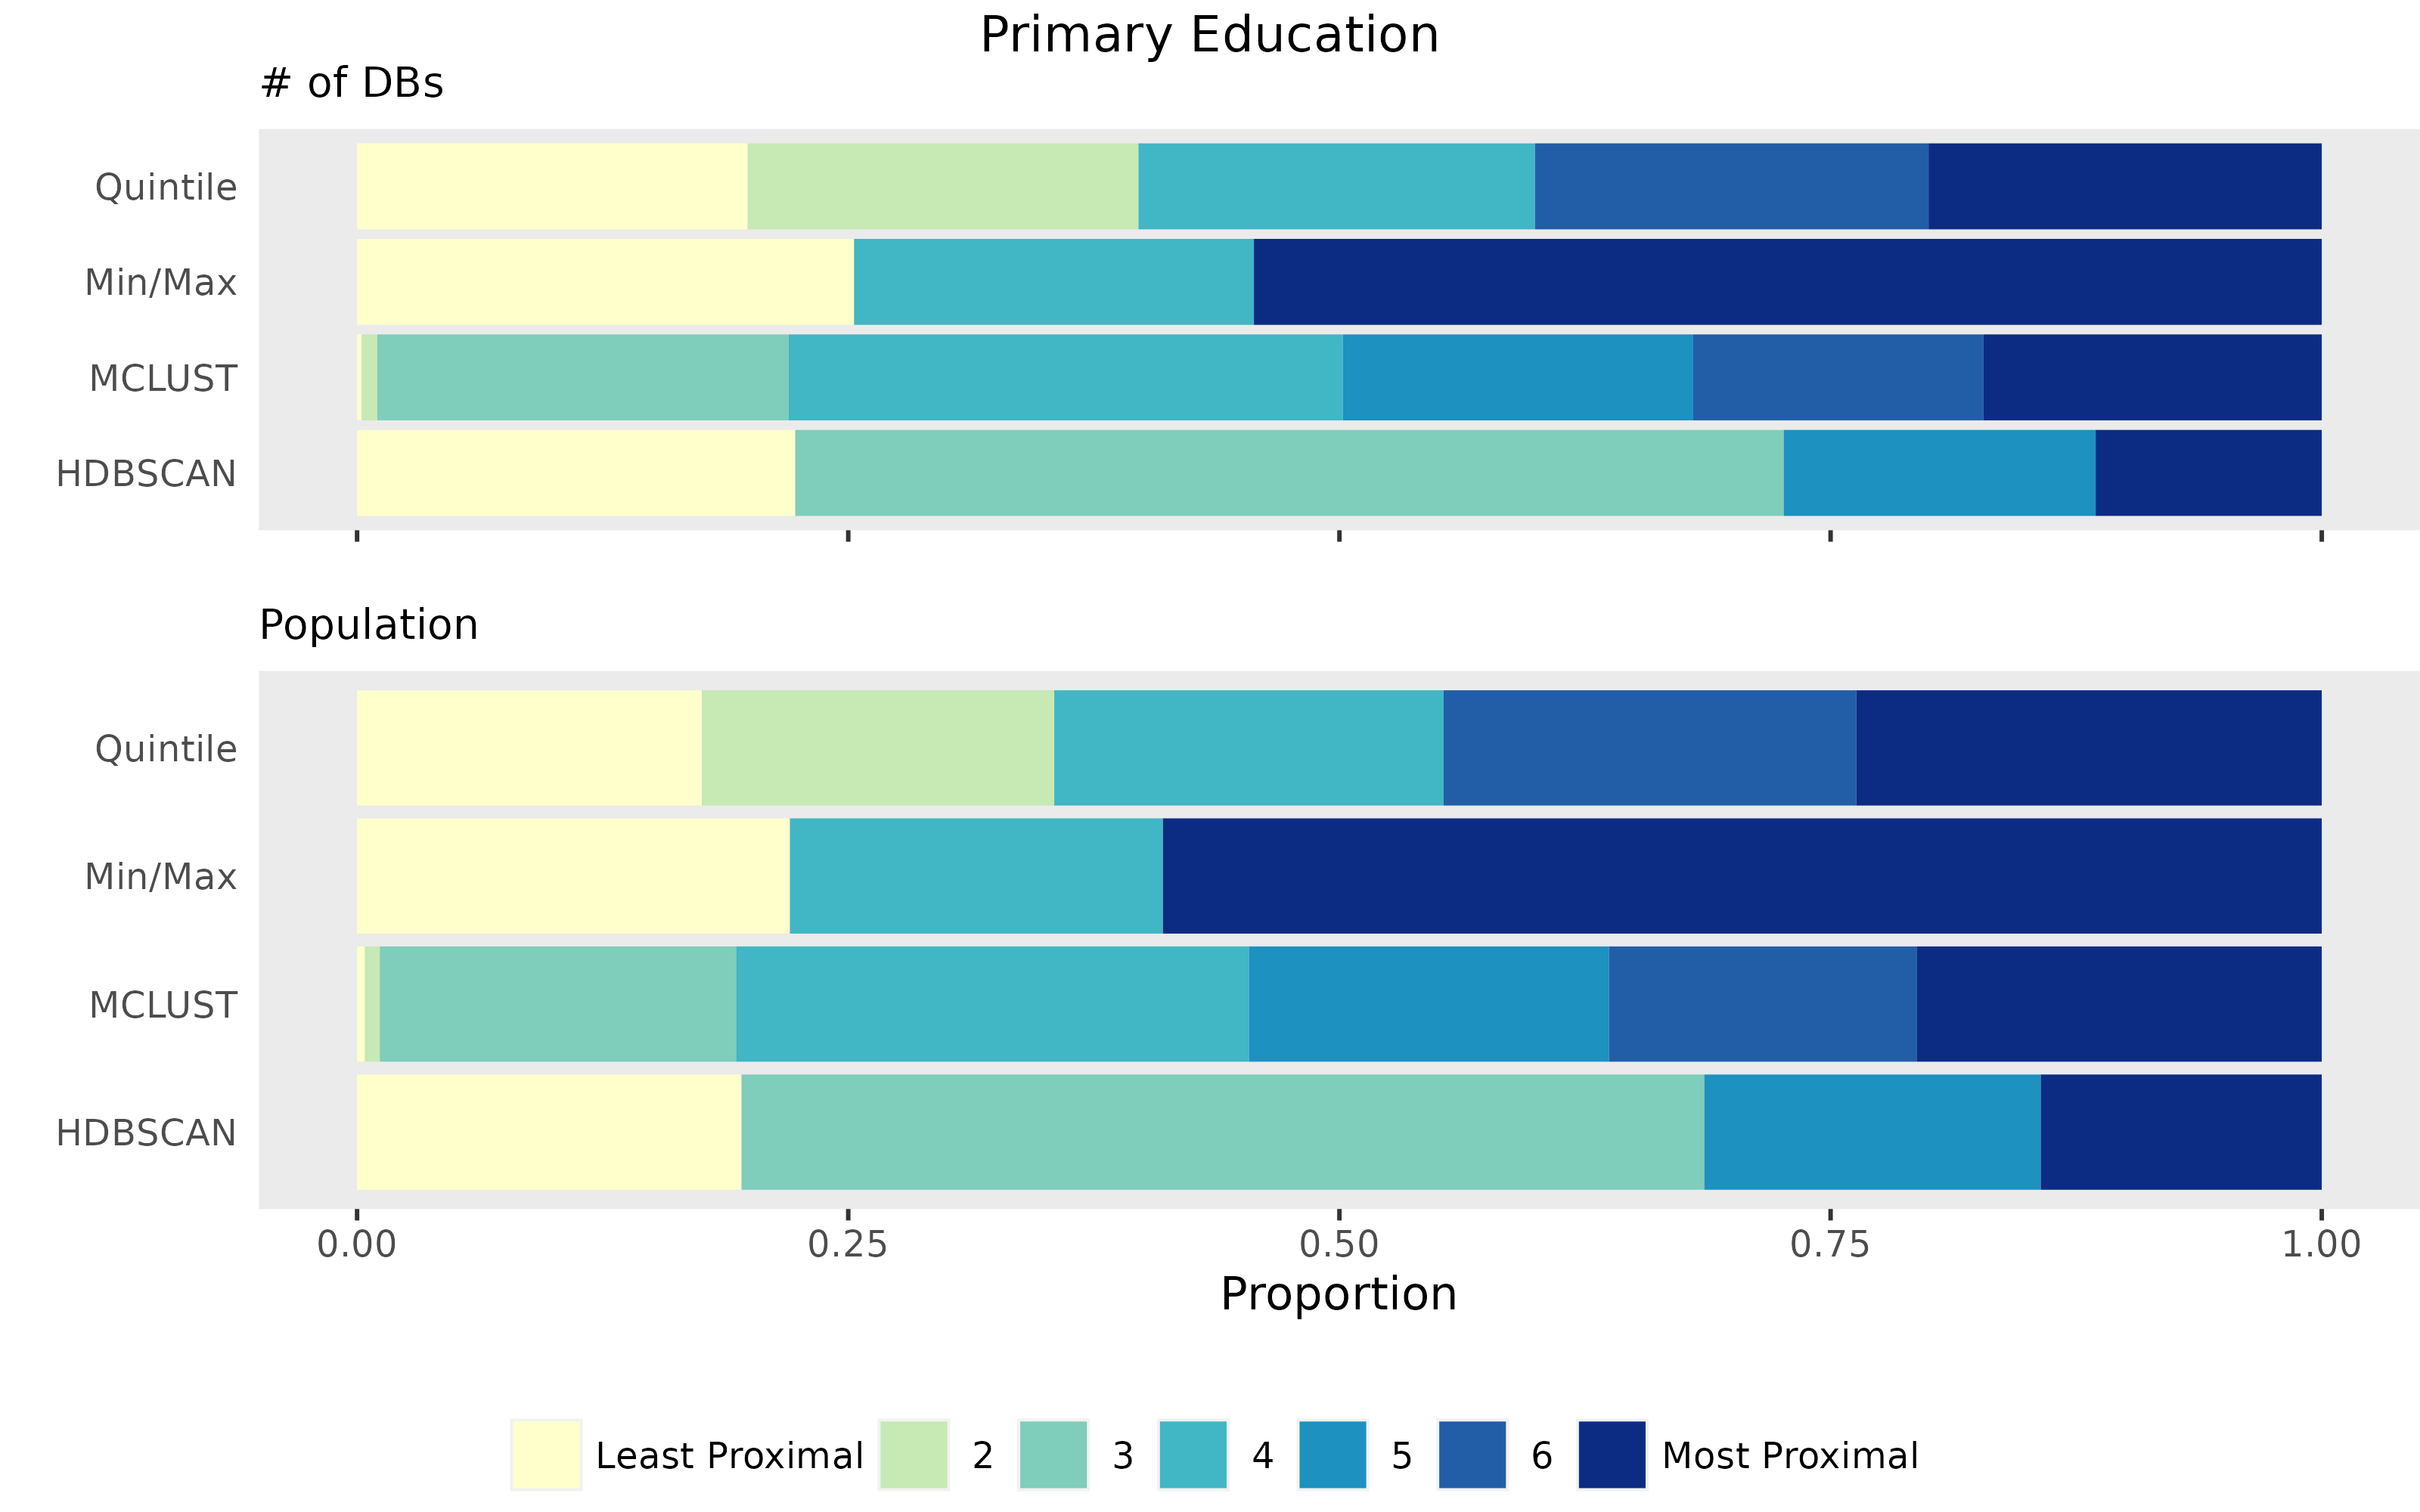
\includegraphics[width=\textwidth]{./barplot_comparison/Primary Education_barplot.png}
\caption[Primary education profile barplot]{Proportion of DBs and population in each cluster for all approaches for the primary education amenity.}\label{prieducbarplot}
\end{figure}










\pagebreak 
%%%%%%%%%%%%%%%%%%%%%%%%%%%%%%%%%%%%%%%%
\section{Discussion}
%%%%%%%%%%%%%%%%%%%%%%%%%%%%%%%%%%%%%%%%




THIS WILL BE DONE IN THE NEXT VERSION  







\subsection{Comparison of Approaches}


















\subsection{Interpretation of Cluster Profiles}
























\pagebreak 
%%%%%%%%%%%%%%%%%%%%%%%%%%%%%%%%%%%%%%%%
\section{Limitations}
%%%%%%%%%%%%%%%%%%%%%%%%%%%%%%%%%%%%%%%%


It is worth noting that since the PMD was only recently released as ``experimental statistics", it is possible that better, more comprehensive ways of calculating the proximity index using additional/different data sources may be developed in the future, which may render our methodology obsolete. 










%\pagebreak 
%%%%%%%%%%%%%%%%%%%%%%%%%%%%%%%%%%%%%%%%
\section{Future Work}
%%%%%%%%%%%%%%%%%%%%%%%%%%%%%%%%%%%%%%%%



There are many other potential avenues for future research in the clustering of the PMD. These include:
\begin{itemize}
\item Forcing the \# of clusters to be the same between all algorithms. 
\item Trying different combinations of variables in multidimensional clustering.
\item Trying additional clustering algorithms. 
\item Clustering on different data transformations. 
\item Sub-clustering - finding some way of dealing with outliers aside from selective models?
\item Soft assignments - having ranges for cutoffs instead of hard cutoffs. 
\end{itemize}









\pagebreak 
%%%%%%%%%%%%%%%%%%%%%%%%%%%%%%%%%%%%%%%%
\section{Conclusion}
%%%%%%%%%%%%%%%%%%%%%%%%%%%%%%%%%%%%%%%%


In conclusion, this project aimed to explore segmentation of continuous proximity measures in the Proximity Measure Database (PMD) developed by Statistics Canada. The goal was to create intuitive and understandable categorical measures for amenities, which could inform decision-making processes for policymakers and urban planners. By categorizing the proximity measures, it becomes easier to prioritize efforts in enhancing access and promoting social and economic sustainability within communities.
\par
The project employed various clustering methods, including HDBSCAN, MixAll, Mclust, and PAM K-means algorithms, to determine optimal cutoff values and cluster boundaries for each amenity. Additionally, clustering validation metrics such as the silhouette coefficient, Dunn index, Calinski-Harabasz, and Davies-Bouldin were used to evaluate the performance of each clustering technique and determine the appropriate number of clusters.
\par
The results showed that the clustering techniques produced diverse outcomes, and there was no single algorithm that consistently outperformed others. Therefore, multiple techniques were utilized to ensure robustness and comprehensive exploration of the data.
\par
Furthermore, cluster profiling was conducted to analyze the characteristics of each cluster, including the number of dissemination blocks, DB population, IoR, and provincial breakdown. This analysis provided insights into the heterogeneity between clusters and the homogeneity within each cluster.
\par
Overall, this project demonstrated the potential of clustering methods in segmenting continuous proximity measures and generating meaningful categorical measures. The results can inform policymakers and urban planners in making informed decisions about the location of amenities and services, thereby enhancing access, social inclusion, and economic development within communities. Further research and analysis can build upon these findings to refine the clustering techniques and explore additional factors that contribute to the characteristics of clusters in the PMD.

















\pagebreak
\section{References}

THIS WILL BE DONE IN THE NEXT VERSION 




\bibliographystyle{apa}
\renewcommand{\bibsection}{}
\bibliography{final_sources.bib}
















\pagebreak
\appendix
\section{Appendix}


\subsection{Successful Methods}\label{appendix:successful}


\subsubsection{K-means (Partitioning Around Medoids - PAM)}

K-means is a clustering algorithm that aims to partition a dataset into K clusters, where each data point belongs to the group with the closest mean. The Partitioning Around Medoids (PAM) variation replaces the concept of `mean' with `medoids' to handle noise and outliers more effectively  (Kaufman and Rousseeuw 1990).
\par
The PAM algorithm, an evolution of the K-means clustering method, operates by selecting K representative objects, or medoids, among the observations of the dataset. These medoids are the most centrally located data points in a cluster, which means the average dissimilarity between a medoid and all other objects within the same cluster is minimized. In contrast to the K-means algorithm, which uses means as cluster centers, PAM's utilization of medoids makes it a robust alternative, less sensitive to noise and outliers.
\par
The PAM algorithm works in two phases: the `build phase' and the `swap phase'. During the build phase, K objects are selected to be the medoids, the dissimilarity matrix is calculated, and every object is assigned to its closest medoid. The swap phase attempts to improve the clustering quality by exchanging selected objects (medoids) and non-selected objects. If the sum of the dissimilarities of all objects to their nearest medoid (the objective function) can be reduced by this swapping, then the swap is carried out. The process continues until the objective function can no longer be decreased, resulting in a set of K representative objects which minimize the sum of the dissimilarities of the observations to their nearest representative object (Kaufman and Rousseeuw 1990).


Results

Show here

Why the Results Aren't Good/Useful
Globular 
Each data point belongs to the cluster whose centroid is nearest. This assumes Euclidean distances are the appropriate measure of similarity



Reason to Implement This Algorithm

The presence of numerous outliers for each amenity within the dataset made k-means PAM an enticing algorithm to try for this project. The robust nature of PAM towards outliers, thanks to its use of medoids as opposed to means makes it less sensitive to noise and therefore more capable of handling this sort of dataset. 





\subsubsection{Gaussian Mixture Models (MCLUST)} 

MCLUST is an R package that provides a comprehensive approach to finite mixture models, providing functions for model-based clustering, classification, and density estimation based on Gaussian Mixture Models (GMMs). GMMs are probabilistic models assuming that the data points in a given dataset are generated from a mixture of Gaussian distributions, with each Gaussian component representing a distinct cluster (Scrucca et al., 2016).
\par
Mclust uses the Expectation-Maximization (EM) algorithm for estimating the parameters. The EM algorithm operates iteratively in two steps:
\begin{enumerate}
\item Expectation (E) Step: Expected values of the component memberships are calculated based on the current parameters.
\item Maximization (M) Step: The log-likelihood function is maximized to update the parameter estimates based on these expected values.
\end{enumerate}
The process is repeated until convergence, providing the parameter estimates for the mixture model. Furthermore, Mclust automatically computes and selects the best model as per the Bayesian Information Criterion (BIC), considering different numbers of clusters and different parameterizations of the covariance matrix (Scrucca et al., 2016).


Results
Show here


The results from the Gaussian Mixture Models (MCLUST) might have been influenced by certain assumptions inherent in this method. Firstly, MCLUST assumes that the data is generated from a mixture of Gaussian distributions, an assumption that might not fully hold for our dataset. While we log-transformed our data to better approximate Gaussian distributions, any deviations from this assumption could lead to less accurate clustering (Scrucca et al., 2016).
\par
Additionally, MCLUST assumes that the different components of the Gaussian mixture model are represented by different clusters in the data. If this assumption does not hold, the resulting clusters may not be meaningful or interpretable. Another key assumption is that the variables within each component are normally distributed and independent, an assumption that may not hold in our univariate dataset. Furthermore, MCLUST uses maximum likelihood estimation, which can be sensitive to initial values and local maxima. Therefore, these assumptions and characteristics could potentially impact the accuracy and usefulness of the results from the MCLUST model (Scrucca et al., 2016).

Reason to Implement This Algorithm
This algorithm was chosen due 




\subsubsection{MixAll}

MixAll is a clustering model that functions on the premise of mixture models. These models assume that data is generated from a combination of probability distributions, which is ideal for handling datasets with diverse distributions or missing values.
\par
The MixAll model is basically a mixture model. Mixture models assume data is generated from a combination of probability distributions. Parameter estimation is achieved by maximizing the observed log-likelihood or integrated log-likelihood for data with missing values. Estimation algorithms like expectation-maximization (EM), SEM, and CEM are used and the default is EM which is highlighted below, involving steps such as imputation, conditional probability calculation, and parameter updates. The EM algorithm iteratively performs these steps until convergence (Iovleff, 2019) .
\par
Steps of the EM Algorithm:
\begin{enumerate}
\item I step: Impute the missing values $x^{m}_{i}$ using the current MAP value provided by the current parameter $\theta^{m-1}$.
\item E step: Compute the current conditional probabilities $t^{m}_{ik}$ for $i = 1, \ldots, n$ and $k = 1, \ldots, K$ using the current parameter $\theta^{m-1}$.
\item M step: Update the maximum likelihood estimate $\theta^{m}$ of $\theta$ using the conditional probabilities $t^{m}_{ik}$ as conditional mixing weights, aiming to maximize the log-likelihood function, where $t^{m} = (t^{m}_{ik}, i = 1, \ldots, n, k = 1, \ldots, K)$.
\item Parameter update: The updated expression of mixture proportions $p^{m}_{k}$ for $k = 1, \ldots, K$ are computed. Detailed formulas for updating the parameters $\lambda_{k}$ and $\alpha$ depend on the component parameterization (Iovleff, 2019).
\end{enumerate}

Results
Show here

Why the Results Aren't Good/Useful
The MixAll algorithm's assumptions might have influenced our results. Specifically, the \texttt{clusterDiagGaussian()} function assumes variable independence, expecting multivariate data for clustering, while our data is univariate, possibly leading to less meaningful clusters.
\par
The model also presupposes data generated from a Gaussian mixture. Although we approximated Gaussian distributions by log transforming our data, minor deviations could still affect the model's performance. Another consideration is that the algorithm handles varied standard deviations within each component. If our univariate data doesn't meet this assumption, it might distort the clusters (Iovleff, 2019).
\par
This algorithm was chosen due to its capabilities of imputing missing values, a feature required when dealing with our data which contained many NAs. MixAll's efficient handling of datasets with diverse distributions made it a suitable choice, especially after transforming our data, which originally had a right-skewed distribution into a more normal-looking distribution via log transformation.







\subsubsection{Multivariate - ClustImpute}

ClustImpute algorithm on multi-dimensional, log-scaled proximity measures. Other variables used for this clustering along with the one amenity at a time include:
\begin{itemize}
\item ``CSD\_AREA''
\item ``PMS\_CSDPOP''
\item ``PMS\_DBPOP''
\item ``IOR\_Index\_of\_remoteness''
\end{itemize}

These variables were scaled from 0-1 prior to clustering.
This algorithm ``draws the missing values iteratively based on the current cluster assignment so that correlations are considered on this level''. Also, ``penalizing weights are imposed on imputed values and successively decreased (to zero) as the missing data imputation gets better''. The idea is that the missing value is imputed by those other observations that are more similar to it (ie. in the same cluster).
\par
Algorithm Steps:
\begin{enumerate}
\item It replaces all NAs by random imputation, i.e., for each variable with missings, it draws from the marginal distribution of this variable not taking into account any correlations with other variables 
\item Weights $<$ 1 are used to adjust the scale of an observation that was generated in step 1. The weights are calculated by a (linear) weight function that starts near zero and converges to 1 at n\_end. 
\item A k-means clustering is performed with a number of c\_steps steps starting with a random initialization. 
\item The values from step 2 are replaced by new draws conditionally on the assigned cluster from step 3. 
\item Steps 2-4 are repeated nr\_iter times in total. The k-means clustering in step 3 uses the previous cluster centroids for initialization. 
\item After the last draws a final k-means clustering is performed.
\end{enumerate}

Result 






\subsubsection{Multivariate - VarSelLCM}

The varselLCM (Variable Selection in Latent Class Models) clustering algorithm is a method that combines latent class modeling with variable selection techniques to identify meaningful clusters in data (Marbac \& Sedki, 2017). This method has been applied on all the amenity proximity measures together.
\par
Due to the significant presence of NA values in the dataset, it is necessary to utilize an algorithm that can cluster the data without the need for imputing these NA values. Imputing the NA values in this case could have a substantial impact on the resulting clusters.
\par
Moreover, it is not feasible to simply remove the NA values from all columns in the dataset. This approach would lead to a significant reduction in the amount of available data. Additionally, the presence of missing values in one column can affect the available values in other columns, making it impractical to remove NA values indiscriminately from the dataset.
\par
\begin{enumerate}
\item Data Preparation: The algorithm takes as input a dataset consisting of categorical variables. It is assumed that the data is generated from an underlying latent class structure, where each observation belongs to a specific latent class.
\item Model Initialization: The algorithm begins by randomly assigning observations to different latent classes. It initializes the model parameters, including the class probabilities and the conditional probabilities of each variable within each class.
\item Expectation-Maximization (EM) Algorithm: The varselLCM algorithm employs an iterative process based on the EM algorithm. In the expectation step (E-step), the algorithm calculates the probability of each observation belonging to each class based on the current model parameters.
\item Variable Selection: In the maximization step (M-step), the algorithm selects a subset of relevant variables that contribute to the clustering process. It employs a variable selection criterion, such as the Bayesian Information Criterion (BIC), to identify the most informative variables for clustering.
\item Model Update: Once the relevant variables are selected, the algorithm updates the model parameters based on the observed data and the selected variables. It estimates the class probabilities and the conditional probabilities of the selected variables within each class.
\item Iterative Process: Steps 3-5 are repeated iteratively until convergence is achieved. The algorithm continues updating the model parameters and selecting variables until the clustering solution stabilizes.
\item Final Clustering Solution: Once convergence is reached, the algorithm assigns each observation to the latent class with the highest probability. The resulting clustering solution represents a partitioning of the data into distinct clusters based on the selected variables and their associated probabilities within each class (Marbac \& Sedki, 2017).
\end{enumerate}

Initially, VarselLCM was utilized for multivariate clustering. However, upon observing distinct cluster patterns in the data through log transformation, the focus shifted towards univariate clustering. Unfortunately, attempts to apply VarselLCM for univariate clustering were unsuccessful as it did not converge. Consequently, it was not possible to proceed with the technique. 









\subsection{Unsuccessful Methods}

\subsubsection{OPTICS}


OPTICS stands for Ordering Points To Identify Clustering Structure. This algorithm can be seen as a generalization of DBSCAN. A major issue with DBSCAN is that it fails to find clusters of varying density due to fixed eps. This is solved in OPTICS by using an approach of finding reachability of each point from the core points and then deciding the clusters based on reachability plot (Hashmi, 2021). 
\par
Considering the log-transformed data, we observed multiple peaks and troughs, suggesting that the clusters may have varying densities. Therefore, aim to explore the applicability of OPTICS, a clustering technique adept at accommodating varying densities (Hahsler et al., 2019). Also there were a decent amount of outliers in the proximity measures which OPTICS can handle (2.3. Clustering, n.d.).
\par
Relevant terminologies for OPTICS:
\begin{itemize}
\item $\epsilon$, epsilon (eps): is the Maximum distance between to points that can be considered to form a group/cluster.
\item MinPts: is the minimum number of points that must be present near each other within the epsilon ($\epsilon$) range in order for them to all form a group or cluster.
\item Core Point: A point in the data that has at least MinPts number of points nearby within the eps ($\epsilon$) range.
\item Border Point/Non-Core Point: A border point or non-core point is a data point in which there are fewer than the minimum number of points (MinPts) within reach of it (at a distance of eps).
\item Noise: A noise point is a data point in which there isn't a single point within eps of it.
\item Core Distance: Core distance can be less than the predetermined value of, epsilon ($\epsilon$), which is the maximum allowed distance to find MinPts. Core distance denotes the minimum distance needed for a point to become a core point and denotes that the MinPts number of points can be found within this distance.
\item Reachability distance: Reachability Distance is the minimum distance from the cluster's extreme point if the point is outside the core distance, and the core distance is the distance necessary to reach the point from the cluster if it is inside the core distance (Hashmi, 2021).
\end{itemize}

Algorithm Steps:
\begin{enumerate}
\item For the given values of MinPts and eps($\epsilon$). Find out if a point is close to MinPts number of points within a distance less than or equal to eps. Tag it as a Core Point. Update the reachability distance = core distance for all the points within the cluster.
\item If it is not a core point then find out its density connected distance from the nearest cluster. Update the reachability distance.
\item Arrange the data in increasing order of reachability distance for each cluster. The smallest distances come first and represent the dense sections of data and the largest distances come next representing the noise section. This is a special type of dendrogram.
\item Find out the places where a sharp decline is happening in the reachability distance plot.
\item ``Cut'' the plot in the y-axis by a suitable distance to get the clusters (Hashmi, 2021).
\end{enumerate}

Result



The clustering process was applied solely to the employment variable without considering any supplementary explanatory variables. By examining the cutoffs in Table X, it becomes apparent that the clusters overlap and intersect with other clusters. This overlapping and intersecting nature is not suitable for creating distinct profiles. For this reason, the decision was made not to continue with this technique.






\subsubsection{Jenks Natural Break Classification}


The Jenks Natural Breaks Classification (or Optimization) system is a data classification method designed to optimize the arrangement of a set of values into ``natural'' classes. A Natural class is the most optimal class range found ``naturally'' in a data set. Natural breaks are determined with a frequency histogram. Class boundaries are identified as troughs in the data. Many dataset will not have obvious natural breaks which means that this method would tend to show breaks where none really exists (Jenks Natural Breaks Classification - GIS Wiki - the GIS Encyclopedia, 2018.)
\par
By attempting to minimize the average deviation of each class from the class mean while maximizing the average deviation of each class from the means of the other classes, the Jenks Natural Breaks Classification method attempts to reduce the variance within classes while enhancing the variance between classes (Wikipedia contributors, 2023).
\par
Jenks Natural Breaks is chosen for application due to the limitation of proximity measures in representing data distribution, specifically when the distribution is not normal. Jenks Natural Breaks, being a non-parametric method, does not assume any specific data distribution and can be applied to a wide range of data types and distributions. This makes it a suitable choice in cases where the proximity measures' distribution deviates from normality. By considering the inherent characteristics of the data, Jenks Natural Breaks can identify natural groupings based on the actual data distribution, enhancing the clustering results. (Geospatial Analysis 6th Edition, 2021 Update - De Smith, Goodchild, Longley and Colleagues, 2021)
\par
Algorithm Steps:
\begin{enumerate}
\item The user selects the attribute, x, to be classified and specifies the number of classes required, k.
\item A set of k‑1 random or uniform values are generated in the range [min\{x\},max\{x\}]. These are used as initial class boundaries. 
\item The mean values for each initial class are computed and the sum of squared deviations of class members from the mean values is computed. The total sum of squared deviations (TSSD) is recorded
\item Individual values in each class are then systematically assigned to adjacent classes by adjusting the class boundaries to see if the TSSD can be reduced. This is an iterative process, which ends when improvement in TSSD falls below a threshold level, i.e. when the within class variance is as small as possible and between class variance is as large as possible. True optimization is not assured. The entire process can be optionally repeated from Step 1 or 2 and TSSD values compared (Geospatial Analysis 6th Edition, 2021 Update - De Smith, Goodchild, Longley and Colleagues, 2021).
\end{enumerate}


Results



The results of the Jenks Natural Break classification are not useful for several reasons. Firstly, when considering employment and childcare, there were variations identified. However, for other amenities, the algorithm consistently suggested 2 or 3 clusters. The problem arises when we observe that the natural breaks for these clusters are within a very narrow range. For example, the first cluster has a range from 0 to 0.0095, and the second cluster has a range from 0.0095 to 0.7452. The remaining data points above this range are grouped into the third cluster. When plotting these clusters on a kernel density plot, we observe that only one cluster is visible. This is because the ranges for the other two clusters are so small that they cannot be effectively visualized. This lack of visibility hinders the usefulness of the classification results.
Moreover, these findings are not helpful for profiling purposes as they ignore the variations in the larger range. Focusing solely on the narrow ranges of the clusters neglects the valuable information and differences present in the broader range of data points.














\pagebreak 
\subsection{Extra Plots and Tables}\label{extra}



\begin{table}[H]
\centering
\resizebox{\textwidth}{!}{
\begin{tabularx}{\textwidth}{|p{2cm}|X|} 
\hline
\textbf{Amenity} & \textbf{Definition} \\
\hline
\textit{Employment} & Measures the closeness of a dissemination block to any dissemination block with a source of employment within a driving distance of 10 km. This measure is derived from the employment counts of all businesses -- that is, all North American Industry Classification (NAICS) codes in the Business Register. \\ 
\hline 
\textit{Grocery} & Measures the closeness of a dissemination block to any dissemination block with a grocery store within a walking distance of 1 km. This measure is derived from the total revenue of all NAICS 4451 businesses in the Business Register. \\ 
\hline 
\textit{Pharmacy} & Measures the closeness of a dissemination block to any dissemination block with a pharmacy or a drug store within a walking distance of 1 km. This measure is derived from the presence of all NAICS 446110 businesses in the Business Register. \\ 
\hline 
\textit{Health care} & Measures the closeness of a dissemination block to any dissemination block with a health care facility within a driving distance of 3 km. This measure is derived from the employment counts of all NAICS 6211, 6212, 6213, 621494, and 622 businesses in the Business Register. \\ 
\hline 
\textit{Child care} & Measures the closeness of a dissemination block to any dissemination block with a child care facility within a walking distance of 1.5 km. This measure is derived from the presence of all NAICS 624410 businesses in the Business Register. \\ 
\hline 
\textit{Primary} \newline \textit{Education} & Measures the proximity to primary education measures the closeness of a dissemination block to any dissemination block with a primary school within a walking distance of 1.5 km. Primary schools are classified as education facilities with an International Standard Classification of education (ISCED) level of 1. The data source is a conglomeration of the Open Database of Education Facilities and other sources of education facilities. \\ 
\hline 
\textit{Secondary} \newline \textit{Education} & Measures the closeness of a dissemination block to any dissemination block with a secondary school within a walking distance of 1.5 km. The data source is a conglomeration of the Open Database of Education Facilities and other sources of education facilities where secondary schools are classified as ISCED2 and/or ISCED3. \\ 
\hline 
\textit{Transit} & Measures the closeness of a dissemination block to any source of public transportation within a 1 km walking distance. This measure is derived from the number of all trips between 7:00 a.m. - 10:00 a.m. from a conglomeration of General Transit Feed Specification (GTFS) data sources. \\ 
\hline 
\textit{Parks} & Measures the closeness of a dissemination block to any dissemination block with a neighborhood park within a 1 km walking distance. This measure is derived from the presence of all parks from a conglomeration of authoritative open data sources and OpenStreetMap. \\ 
\hline 
\textit{Libraries} & Measures the closeness of a dissemination block to any dissemination block with a library within a 1.5 km walking distance. This measure is derived from the presence of all libraries from a conglomeration of open and publicly available data sources. \\ 
\hline 
\textit{Amenity Dense} & An aggregate measure was created to indicate neighbourhoods that have access to basic needs for a family with minors. A dissemination block with access to a grocery store, pharmacy, health care facility, child care facility, primary school, library, public transit stop, and source of employment is referred to as an amenity dense neighbourhood. A high amenity density neighbourhood is defined as an amenity dense neighbourhood that has proximity measure values in the top third of the distribution for each of the eight proximity measures. \\ 
\hline 
\hline
\end{tabularx}
}
\caption[Data dictionary]{Data Dictionary for the PMD.}\label{datadictionary}
\end{table}







\begin{table}[H]
\centering
\resizebox{\textwidth}{!}{
\begin{tabular}{|r|llllllllll|}
  \hline
 & Employment & Pharmacy & Childcare & Healthcare & Grocery & Pri. Educ. & Sec. Educ. & Library & Parks & Transit \\ 
  \hline
1 Dec. & -8.51719 & -4.87961 & -4.82831 & -8.11173 & -4.23361 & -3.44202 & -3.28341 & -2.97789 & -4.35831 & -6.72543 \\ 
  2 Dec. & -7.6009 & -4.61522 & -4.1799 & -7.1309 & -3.80766 & -3.17725 & -3.16534 & -2.88419 & -3.89222 & -5.9145 \\ 
  3 Dec. & -6.57128 & -4.21991 & -3.7214 & -6.2659 & -3.54046 & -2.84215 & -3.02413 & -2.77259 & -3.57913 & -5.3817 \\ 
  4 Dec. & -5.77635 & -3.94248 & -3.35527 & -5.71383 & -3.35527 & -2.6297 & -2.83532 & -2.6479 & -3.28876 & -4.99083 \\ 
  5 Dec. & -5.02069 & -3.66126 & -3.04282 & -5.27851 & -3.13499 & -2.40684 & -2.59561 & -2.50715 & -3.0324 & -4.65646 \\ 
  6 Dec. & -4.35831 & -3.37553 & -2.75357 & -4.89285 & -2.88957 & -2.20184 & -2.3958 & -2.34237 & -2.78872 & -4.32754 \\ 
  7 Dec. & -3.82585 & -3.08347 & -2.46864 & -4.49184 & -2.63109 & -1.98997 & -2.1698 & -2.14644 & -2.53326 & -3.98998 \\ 
  8 Dec. & -3.29954 & -2.74575 & -2.14729 & -3.98998 & -2.31668 & -1.75968 & -1.9018 & -1.90448 & -2.25284 & -3.60087 \\ 
  9 Dec. & -2.62141 & -2.31871 & -1.74183 & -3.3697 & -1.87015 & -1.45629 & -1.54693 & -1.55732 & -1.90046 & -3.11677 \\ 
  Min. & -9.21034 & -9.21034 & -9.21034 & -9.21034 & -8.517193 & -7.600902 & -7.418581 & -8.517193 & -9.21034 & -9.21034 \\ 
  Median & -5.02069 & -3.66126 & -3.04282 & -5.27851 & -3.13499 & -2.40684 & -2.59561 & -2.50715 & -3.0324 & -4.65646 \\ 
  Mean & -5.30642 & -3.60872 & -3.14453 & -5.50353 & -3.08437 & -2.41781 & -2.51013 & -2.36977 & -3.06704 & -4.80398 \\ 
  Max. & 1e-04 & 1e-04 & 1e-04 & 1e-04 & 1e-04 & 1e-04 & 1e-04 & 1e-04 & 1e-04 & 1e-04 \\ 
  Std. Dev. & 2.1556 & 0.9607 & 1.1298 & 1.7612 & 0.9114 & 0.7301 & 0.668 & 0.5789 & 0.9174 & 1.4123 \\ 
  Skew & -0.237 & 0.363 & -0.208 & -0.344 & 0.132 & 0.112 & 0.605 & 1.024 & -0.154 & -0.55 \\ 
  Kurtosis & 2 & 2.54 & 2.43 & 2.53 & 2.85 & 2.32 & 2.63 & 4.14 & 3.04 & 3.21 \\ 
   \hline
\end{tabular}
}
\caption[Log summary table]{Summary statistics of log-transformed numerical variables from the PMD.}\label{logsummary}
\end{table}








\pagebreak

\begin{figure}[H]
\centering
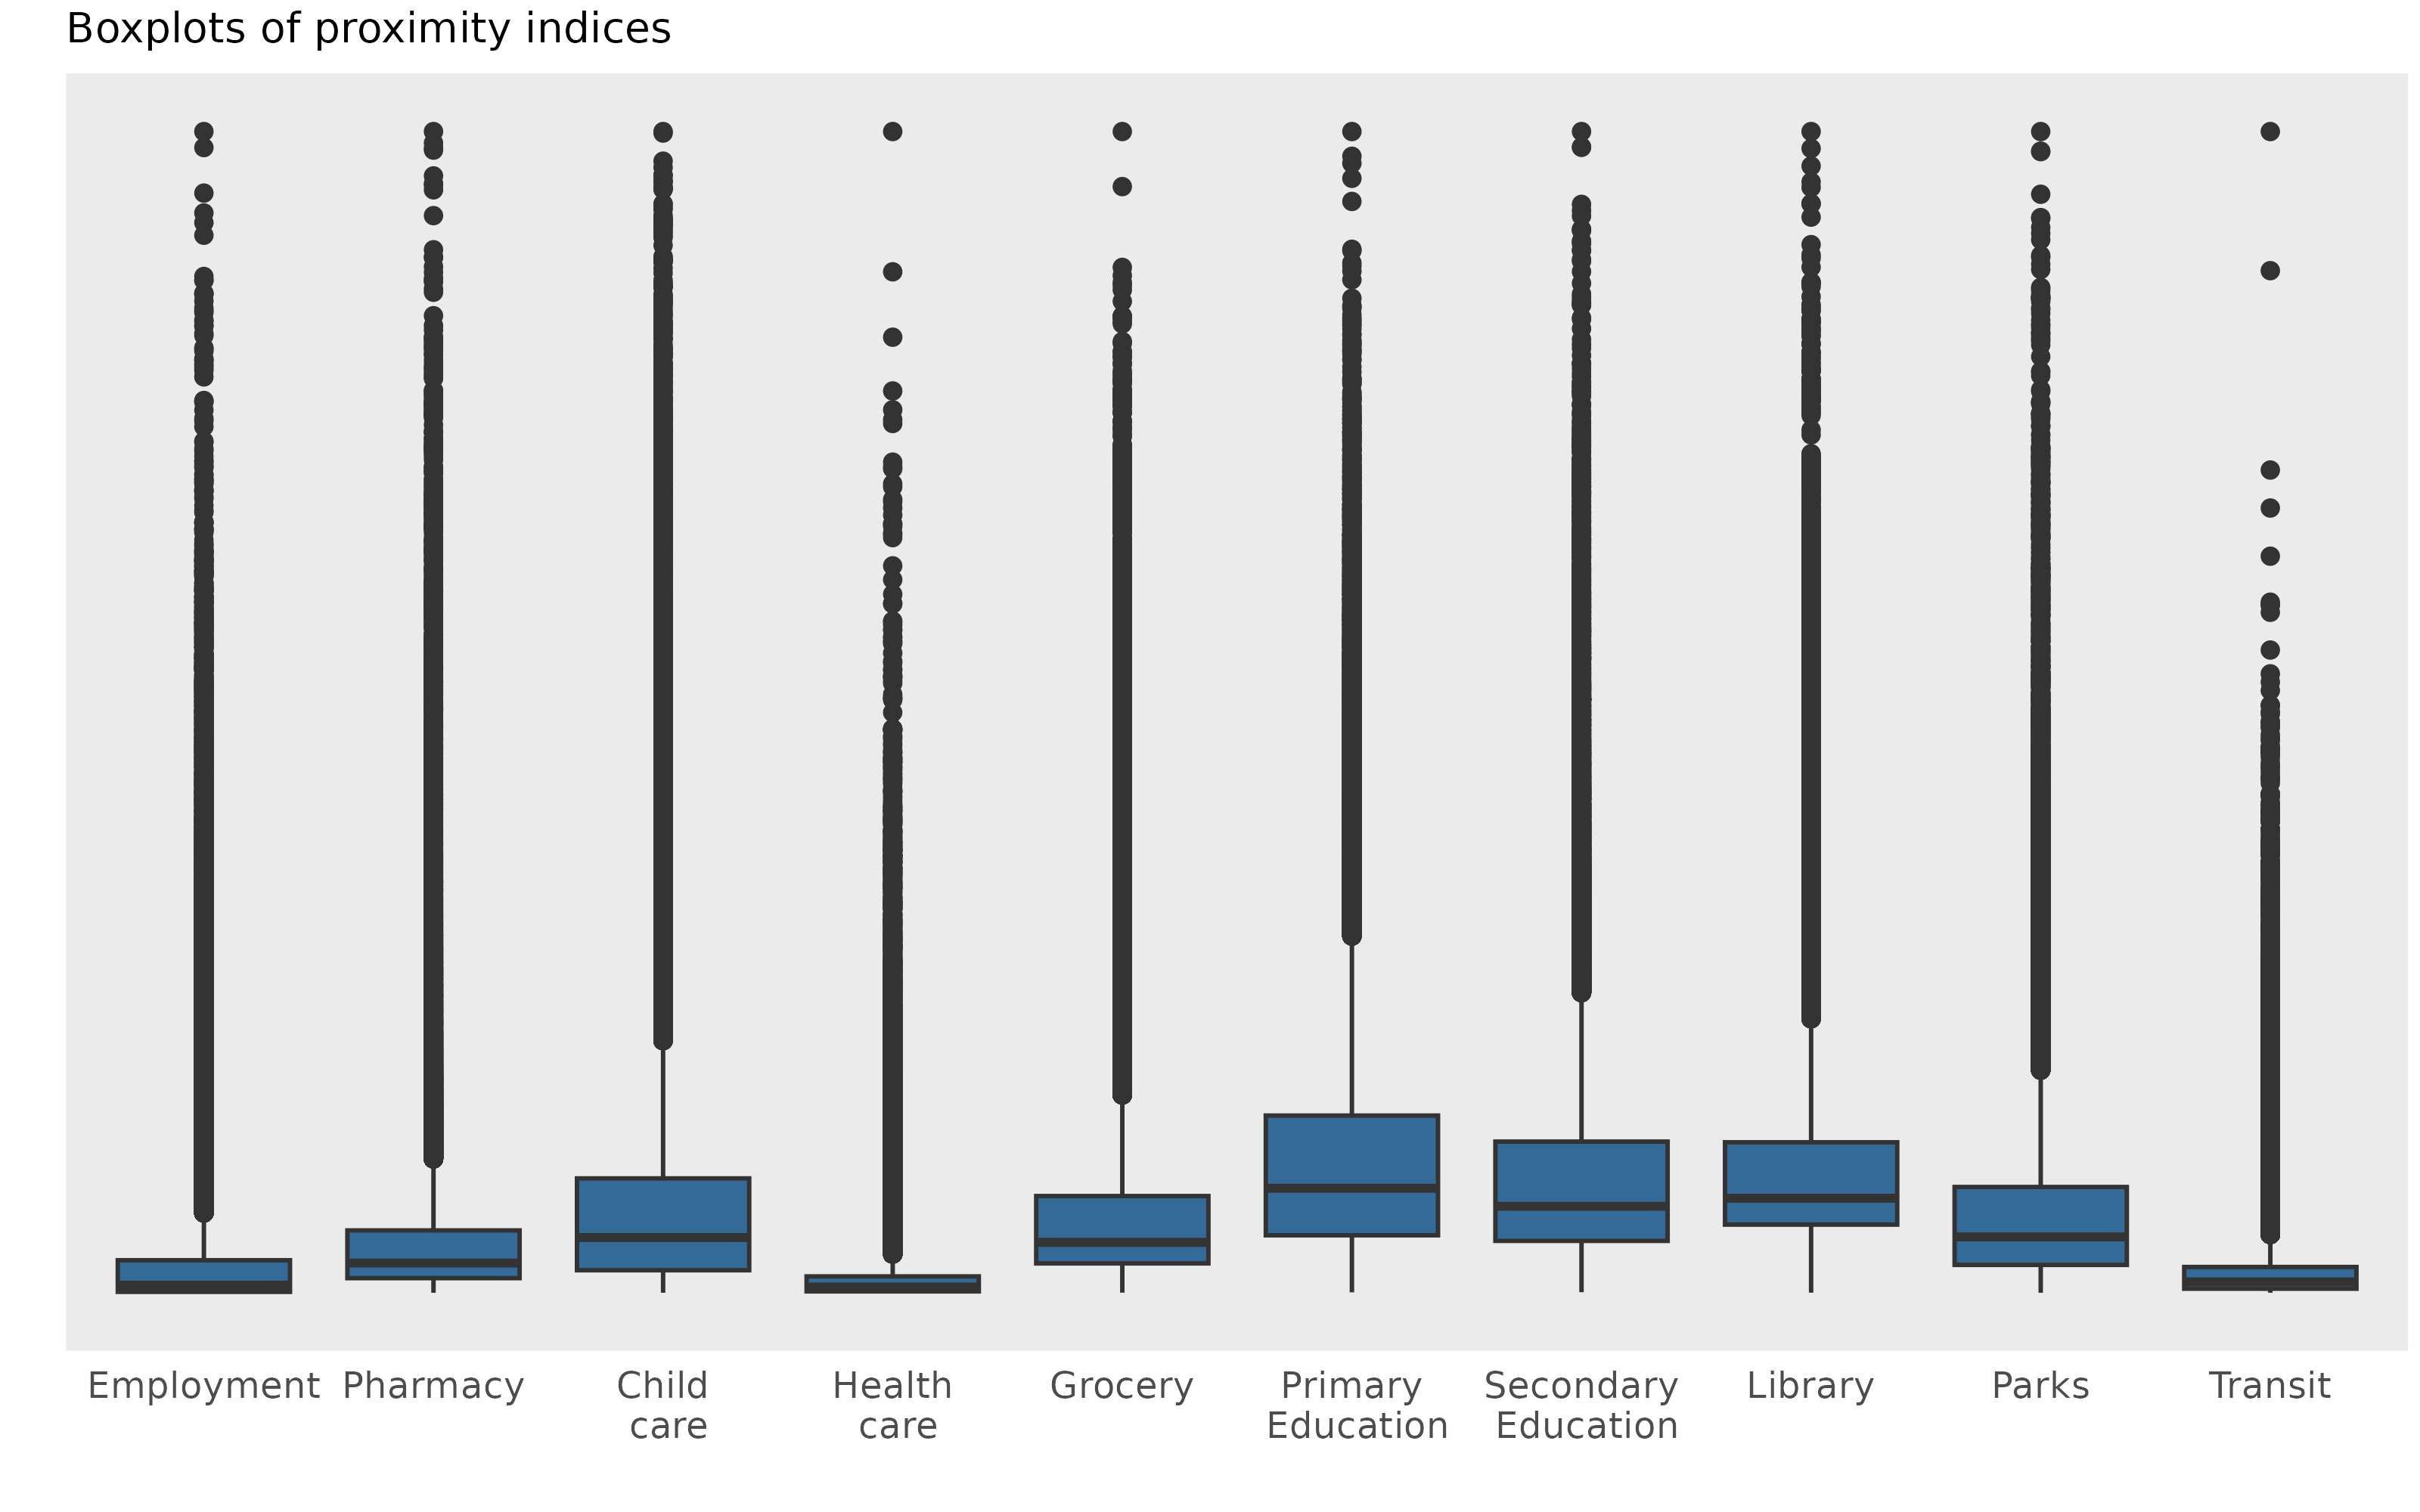
\includegraphics[width=\textwidth]{./outliers/boxplot.png}
\caption[Boxplots of outliers]{Boxplots showing outliers for all ten amenities of the PMD.}\label{boxoutliers}
\end{figure}







\begin{figure}[H]
\centering
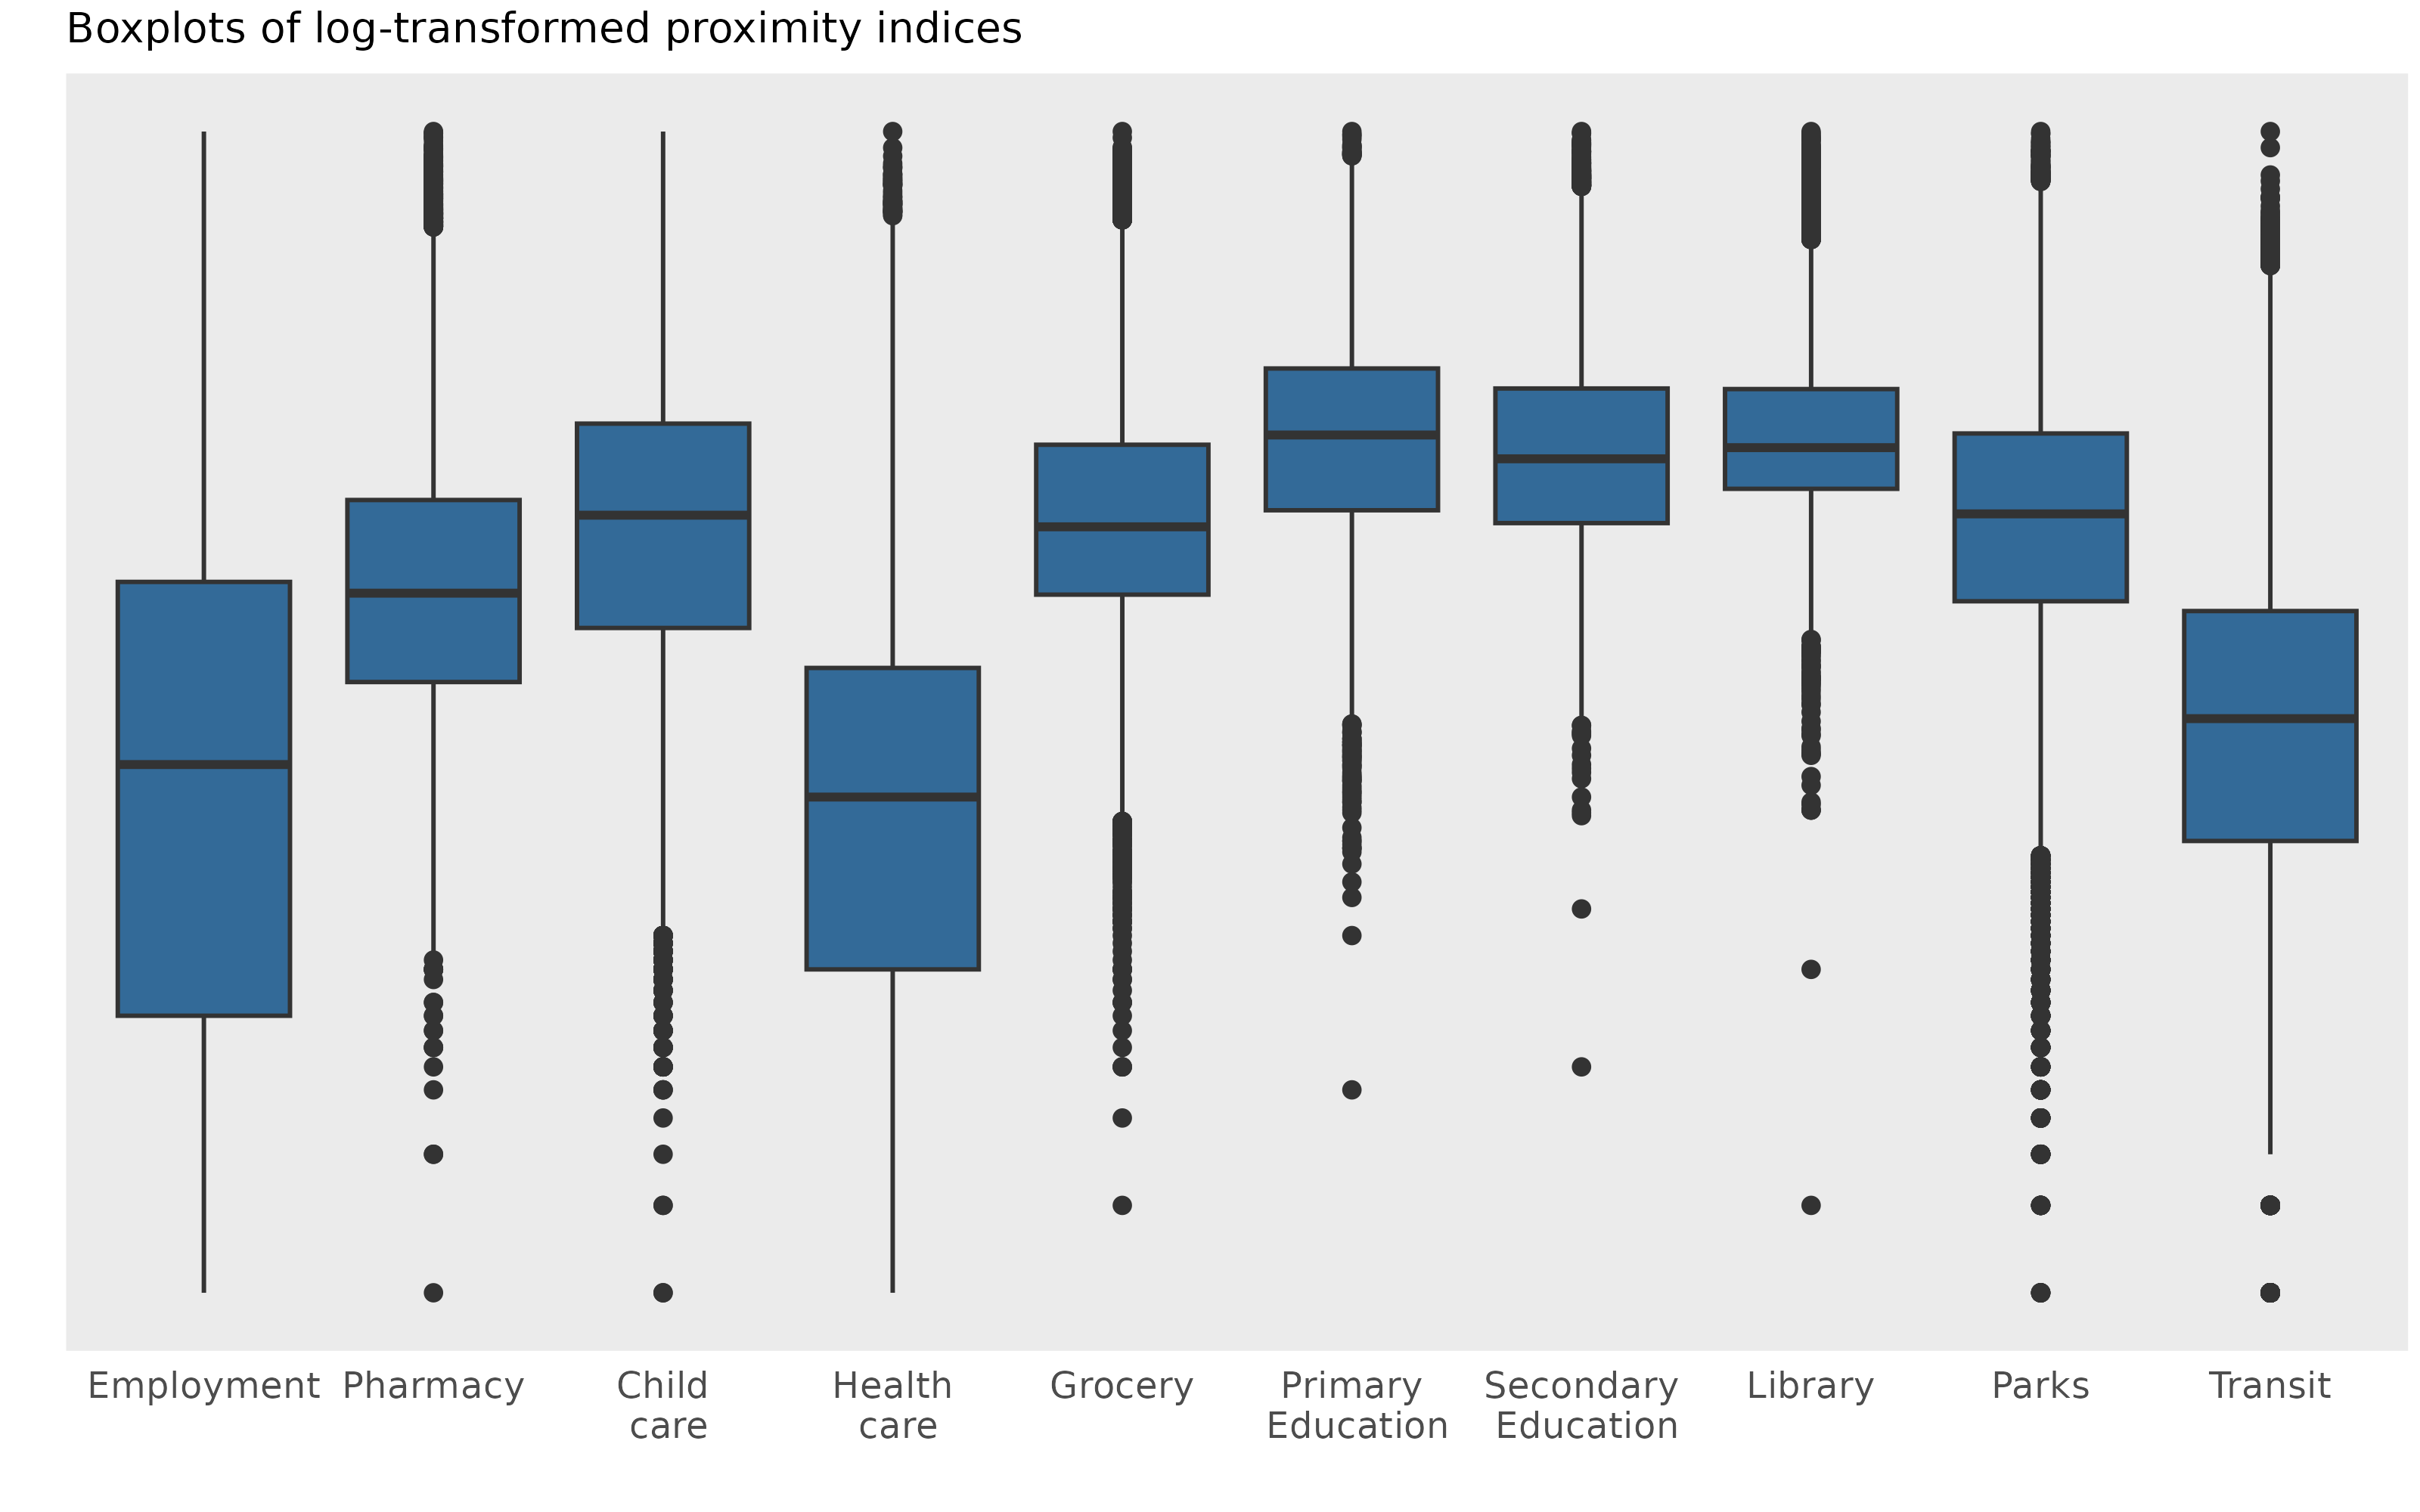
\includegraphics[width=\textwidth]{./outliers/logged_boxplot.png}
\caption[Boxplots of log outliers]{ Boxplots showing outliers for all ten log-transformed amenities of the PMD.}\label{logboxoutliers}
\end{figure}







\begin{figure}[H]
\centering
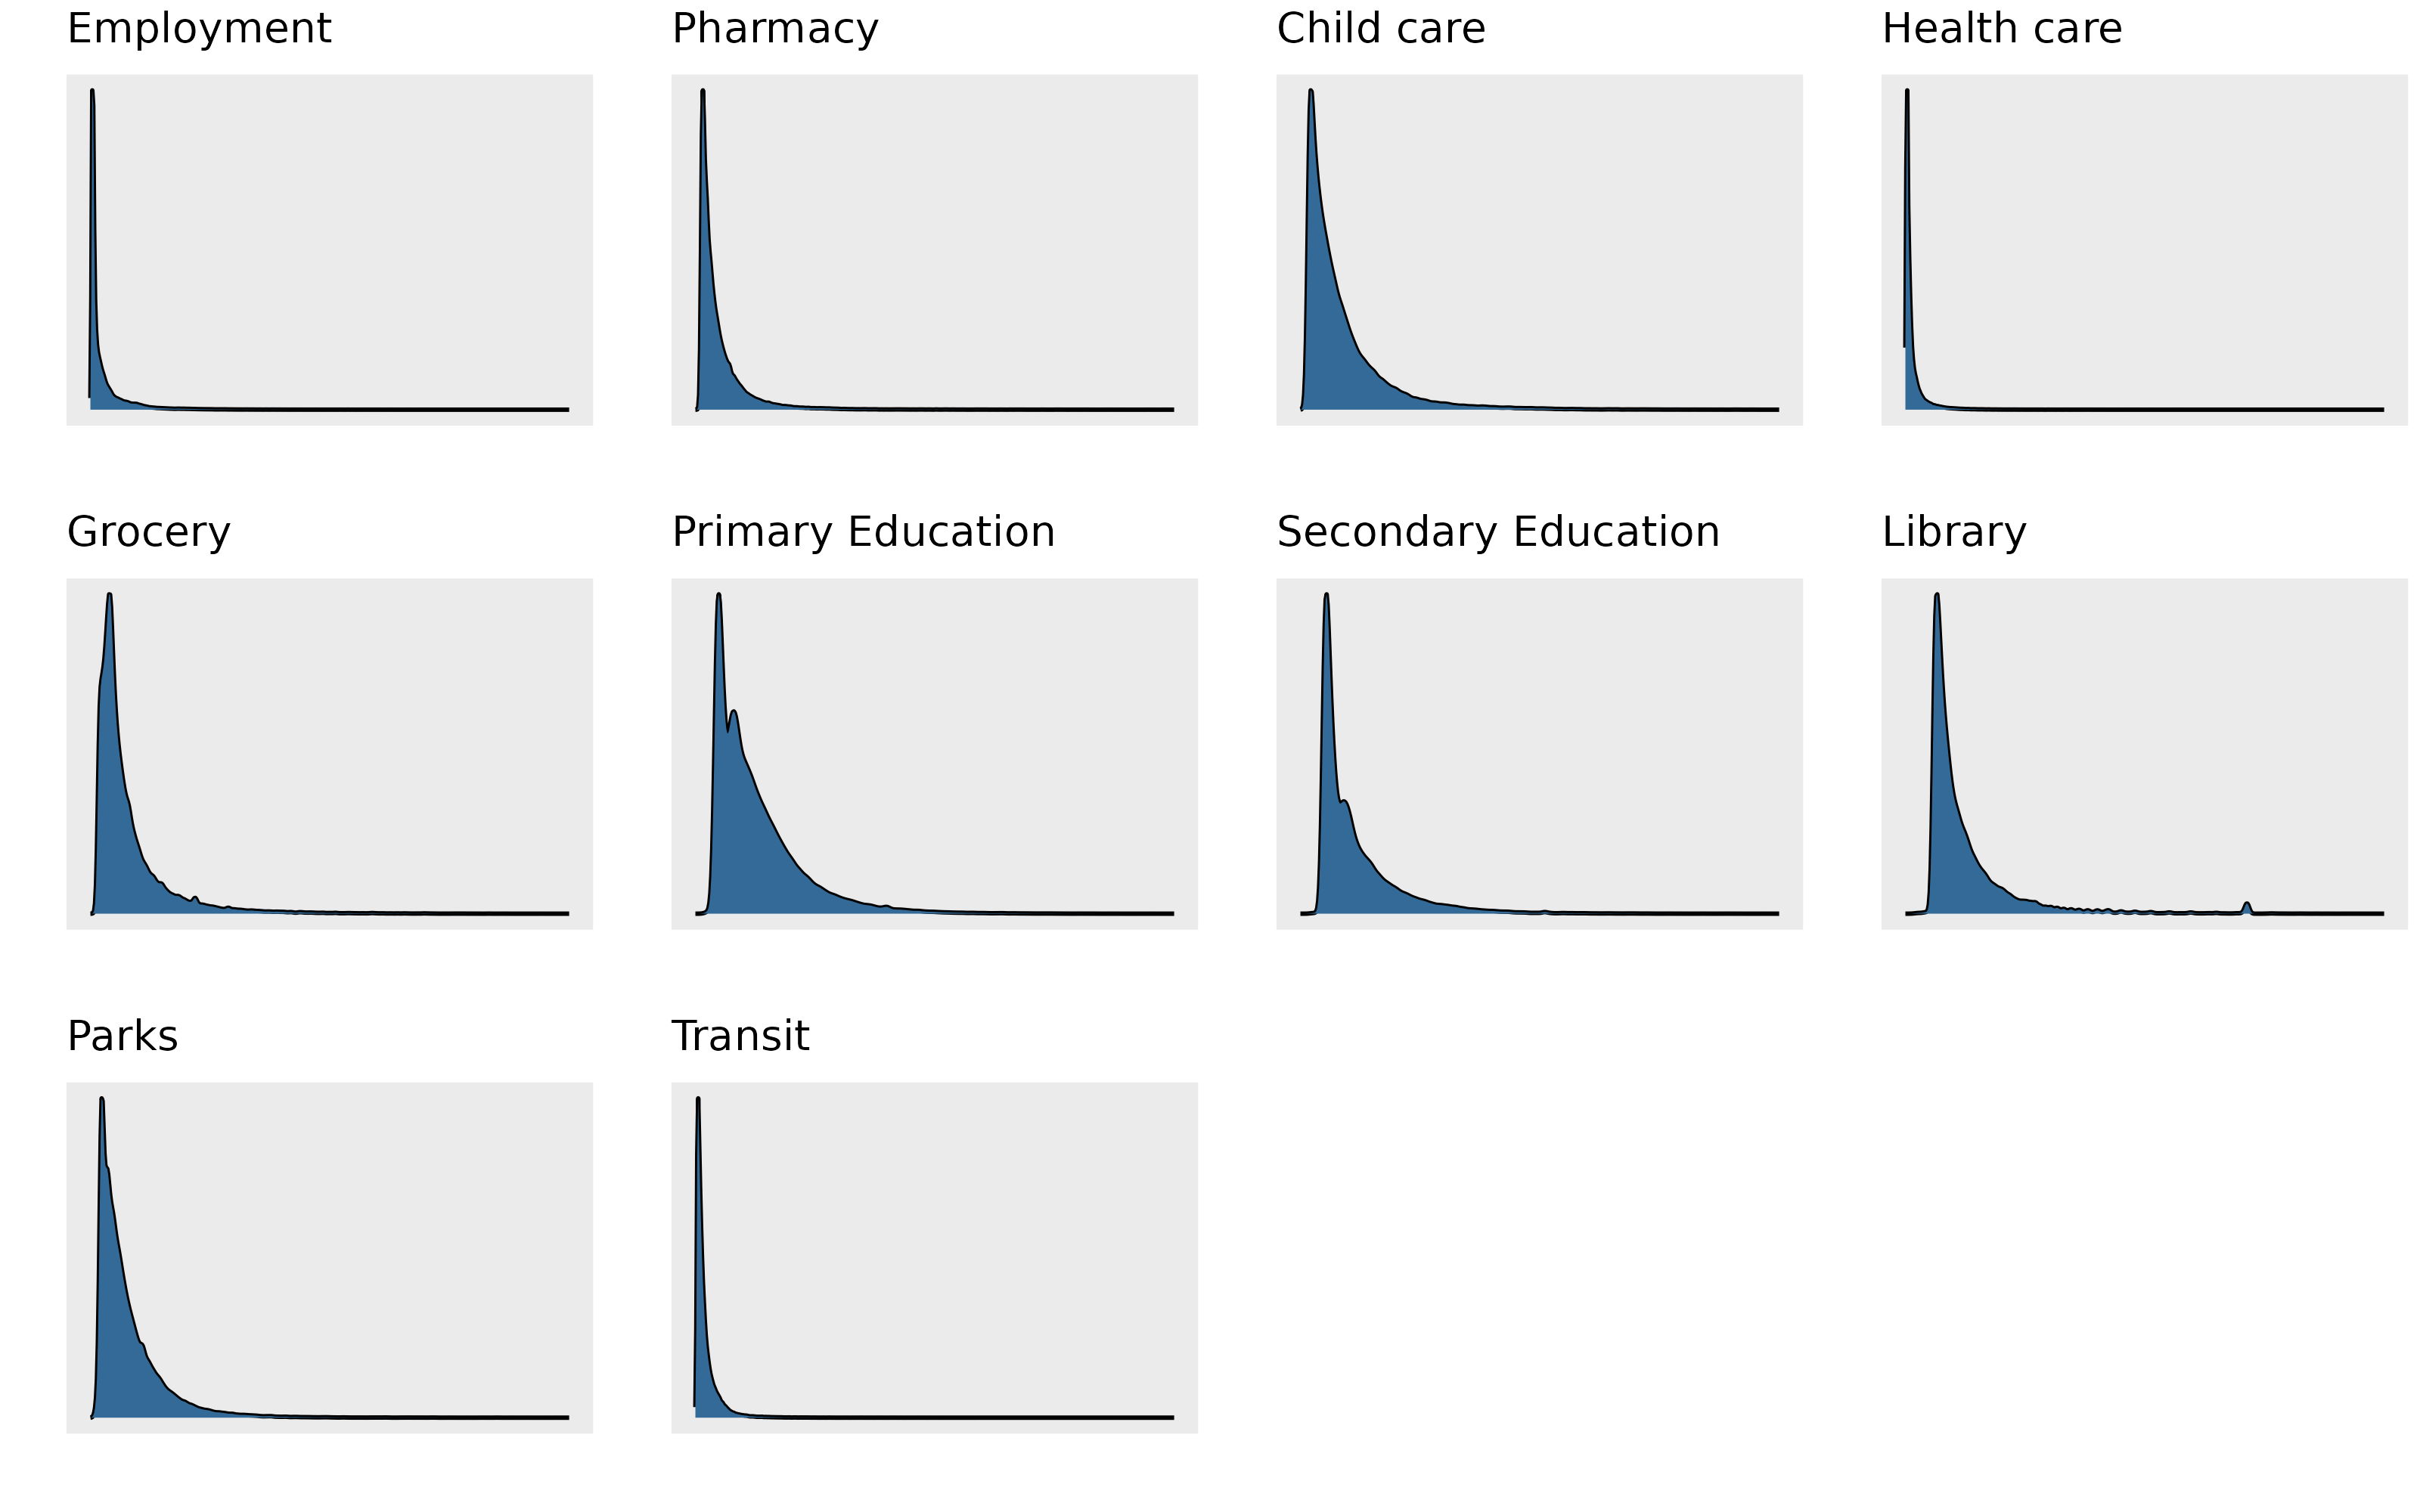
\includegraphics[width=\textwidth]{./distributions/distributions.png}
\caption[Density distributions]{Density distributions for all ten amenities of the PMD.}\label{dendist}
\end{figure}







\begin{figure}[H]
\centering
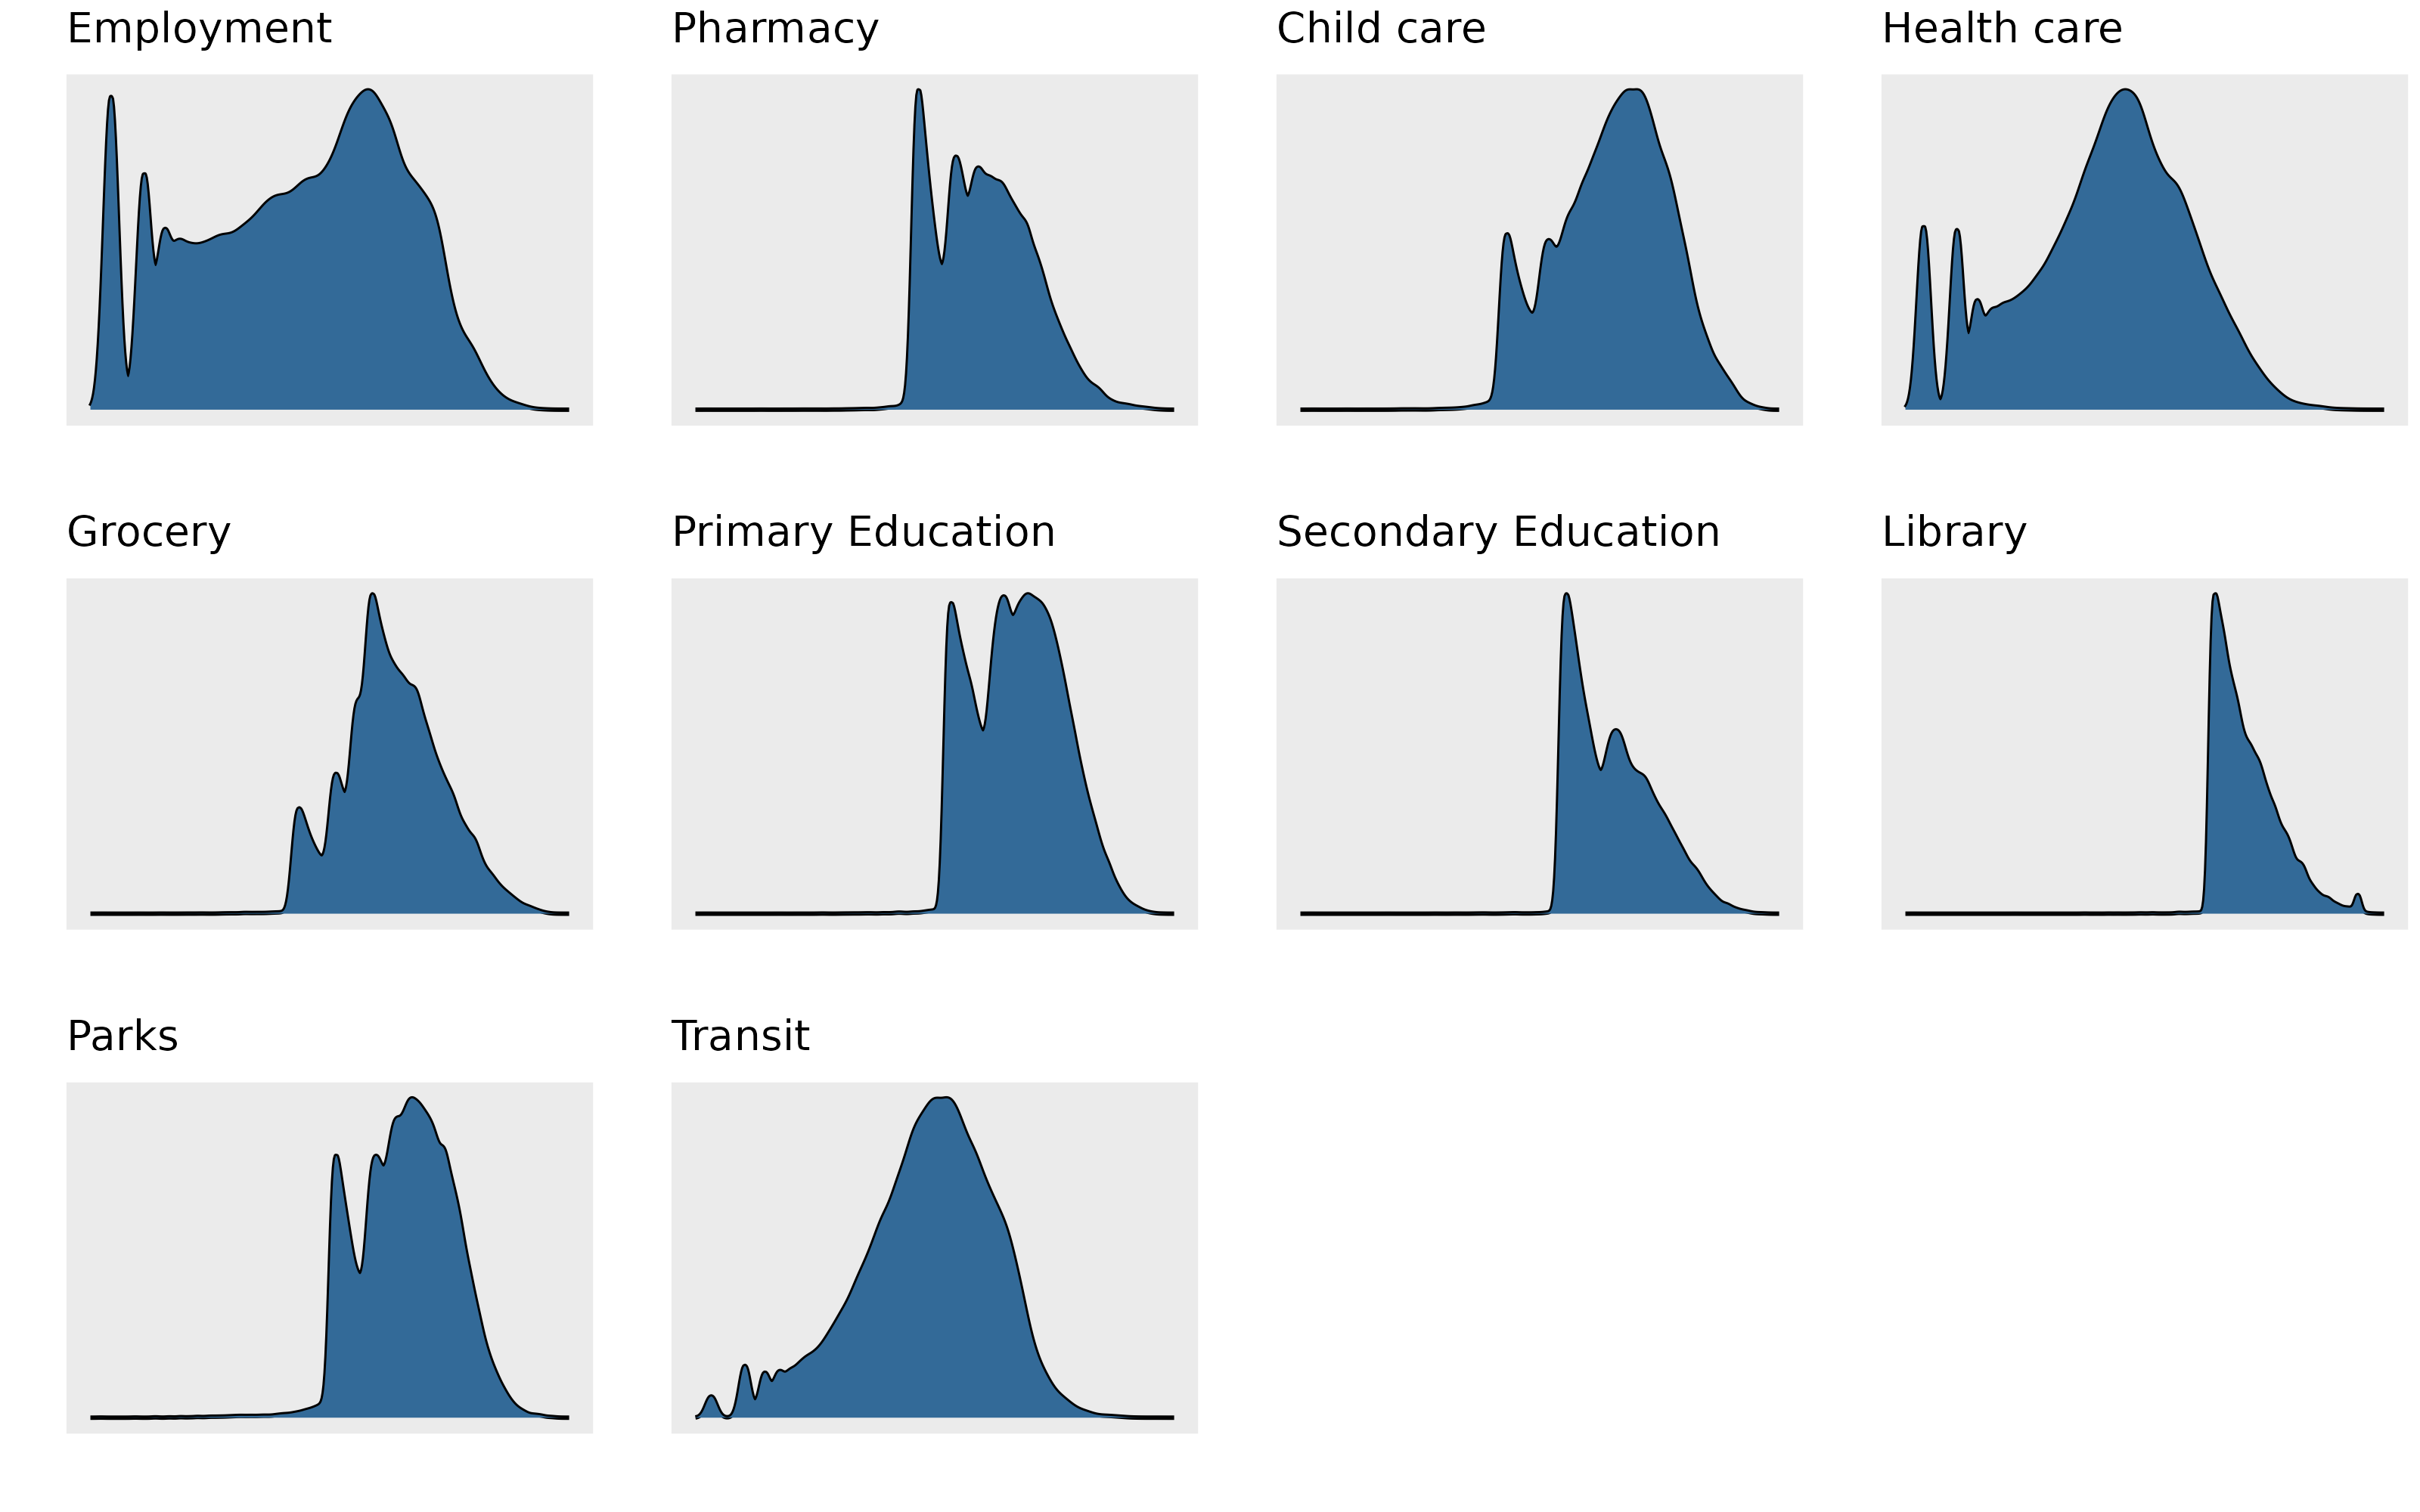
\includegraphics[width=\textwidth]{./distributions/log_distributions.png}
\caption[Log density distributions]{ Log-transformed density distributions for all ten amenities of the PMD.}\label{logdendist}
\end{figure}







\begin{figure}[H]
\centering
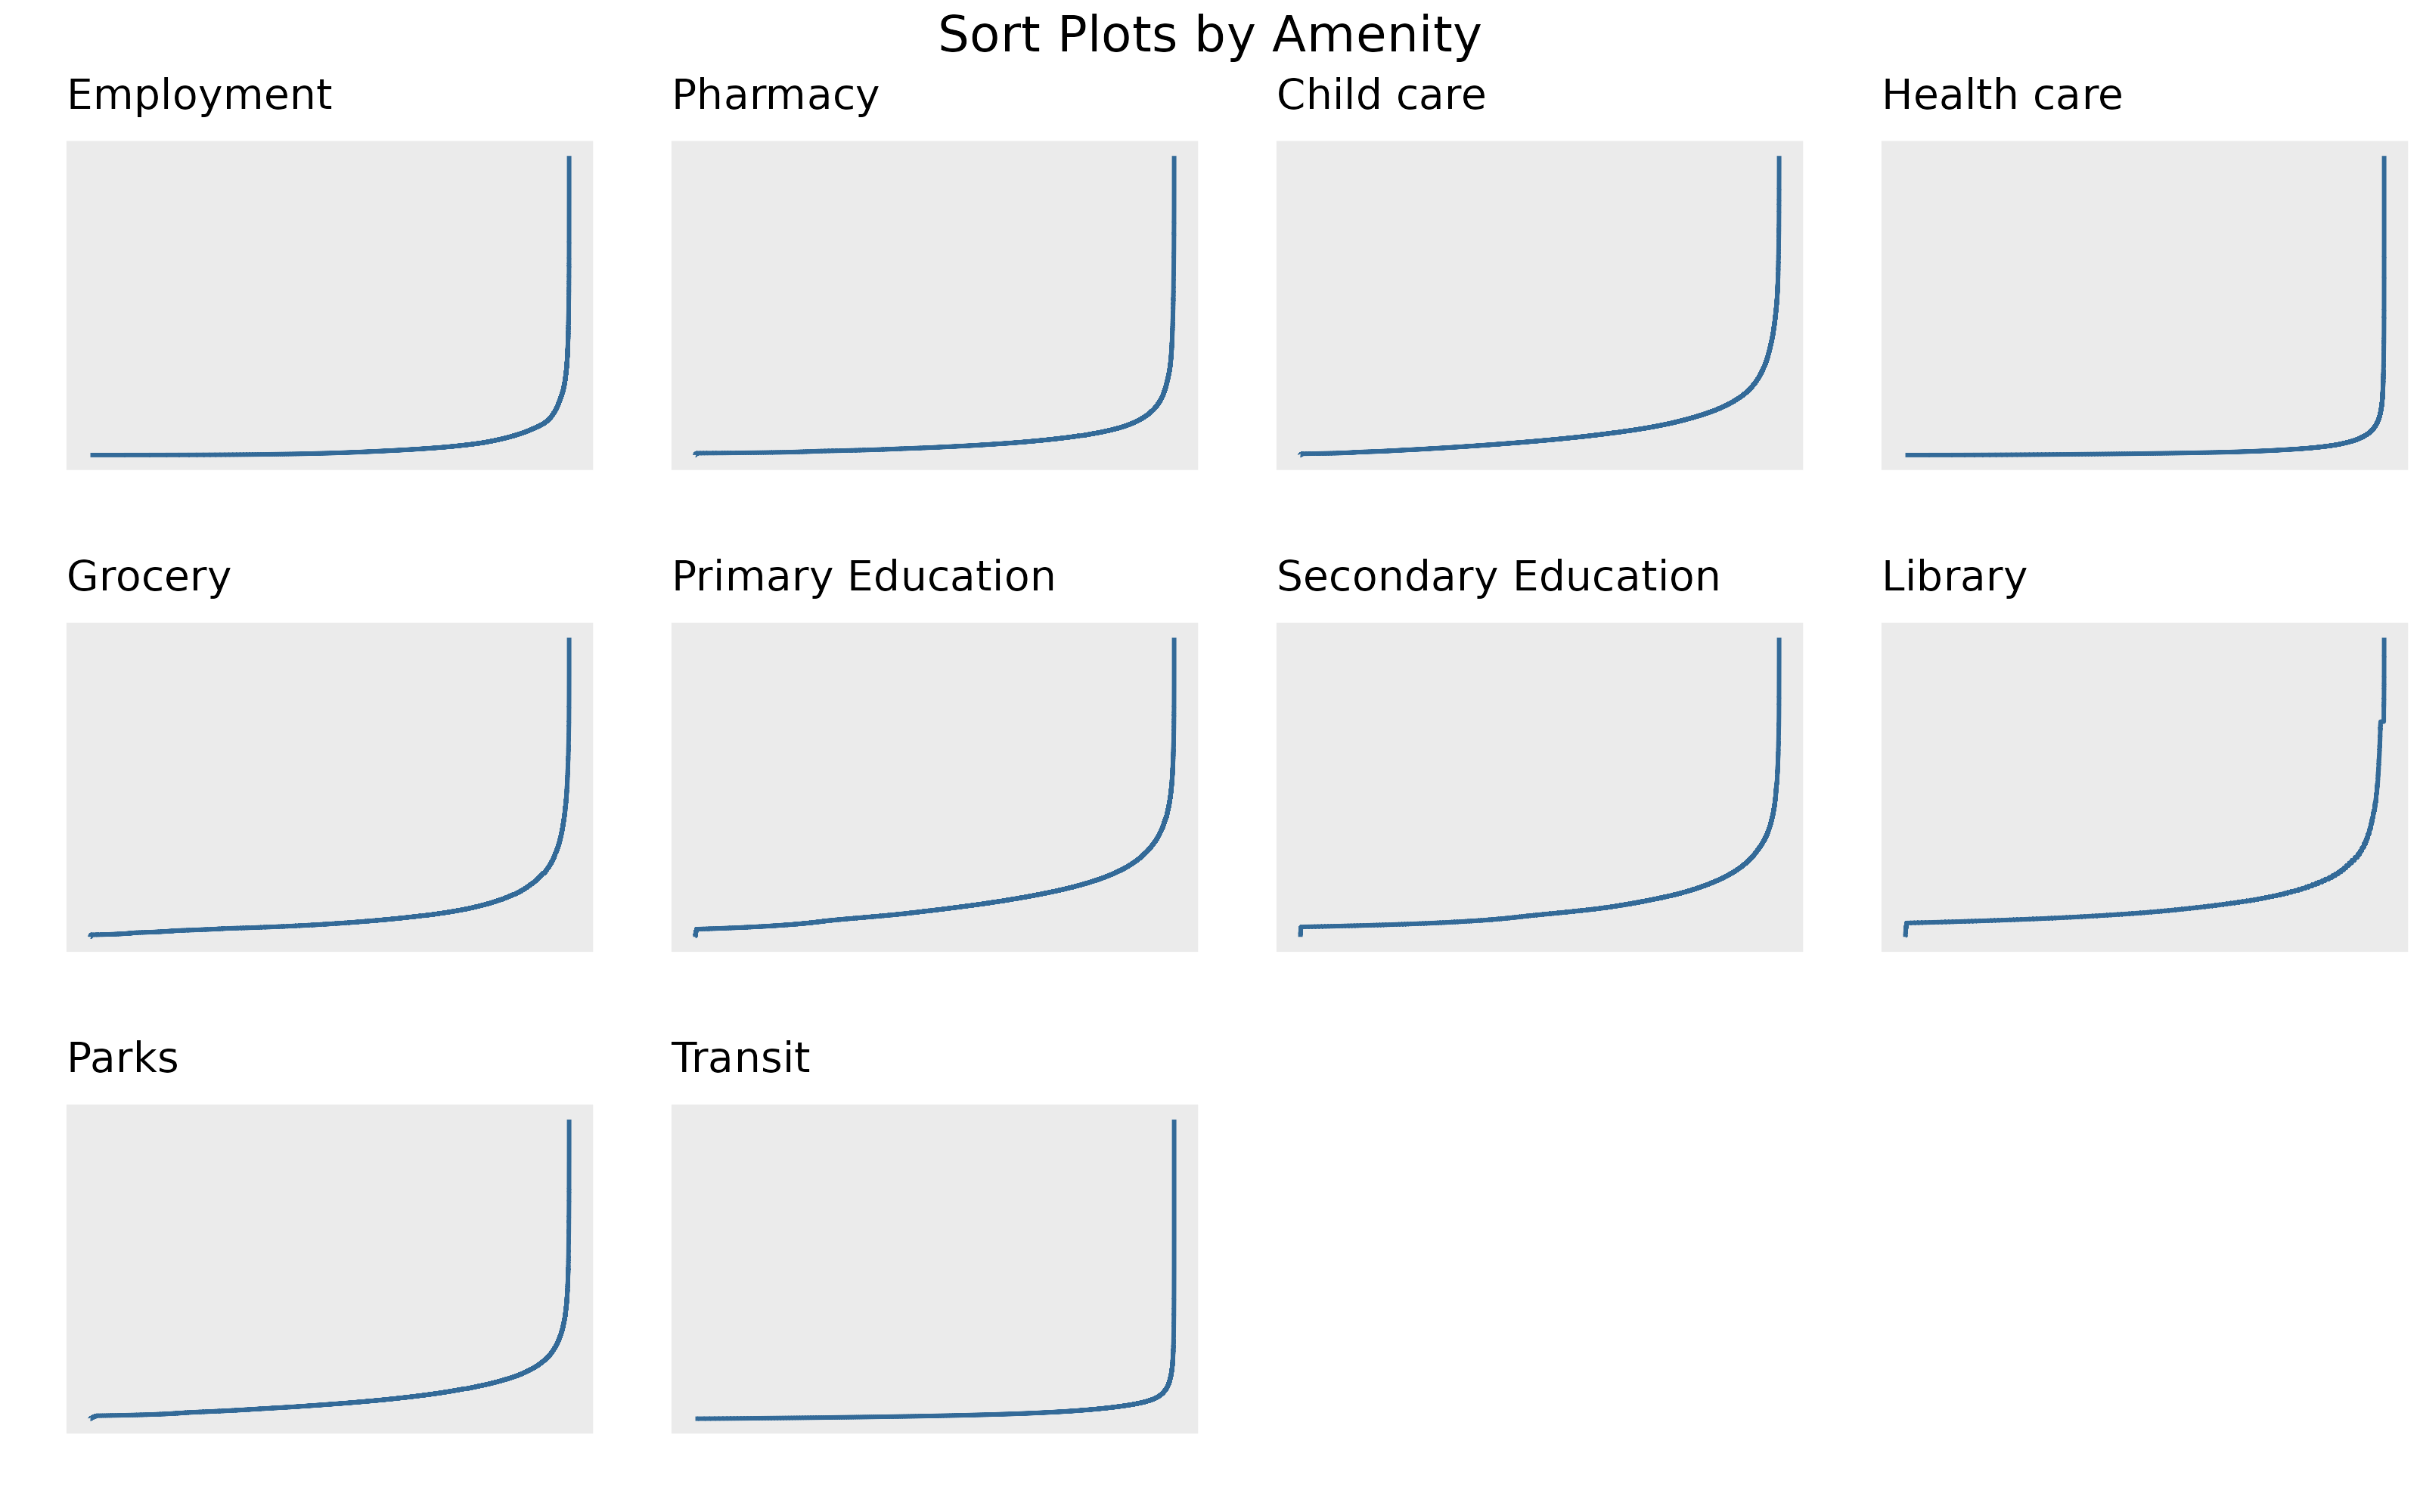
\includegraphics[width=\textwidth]{./sort_plot/sort_plot.png}
\caption[Sort plots]{Sort plots for each amenity in the PMD. }\label{sortplots}
\end{figure}







\begin{figure}[H]
\centering
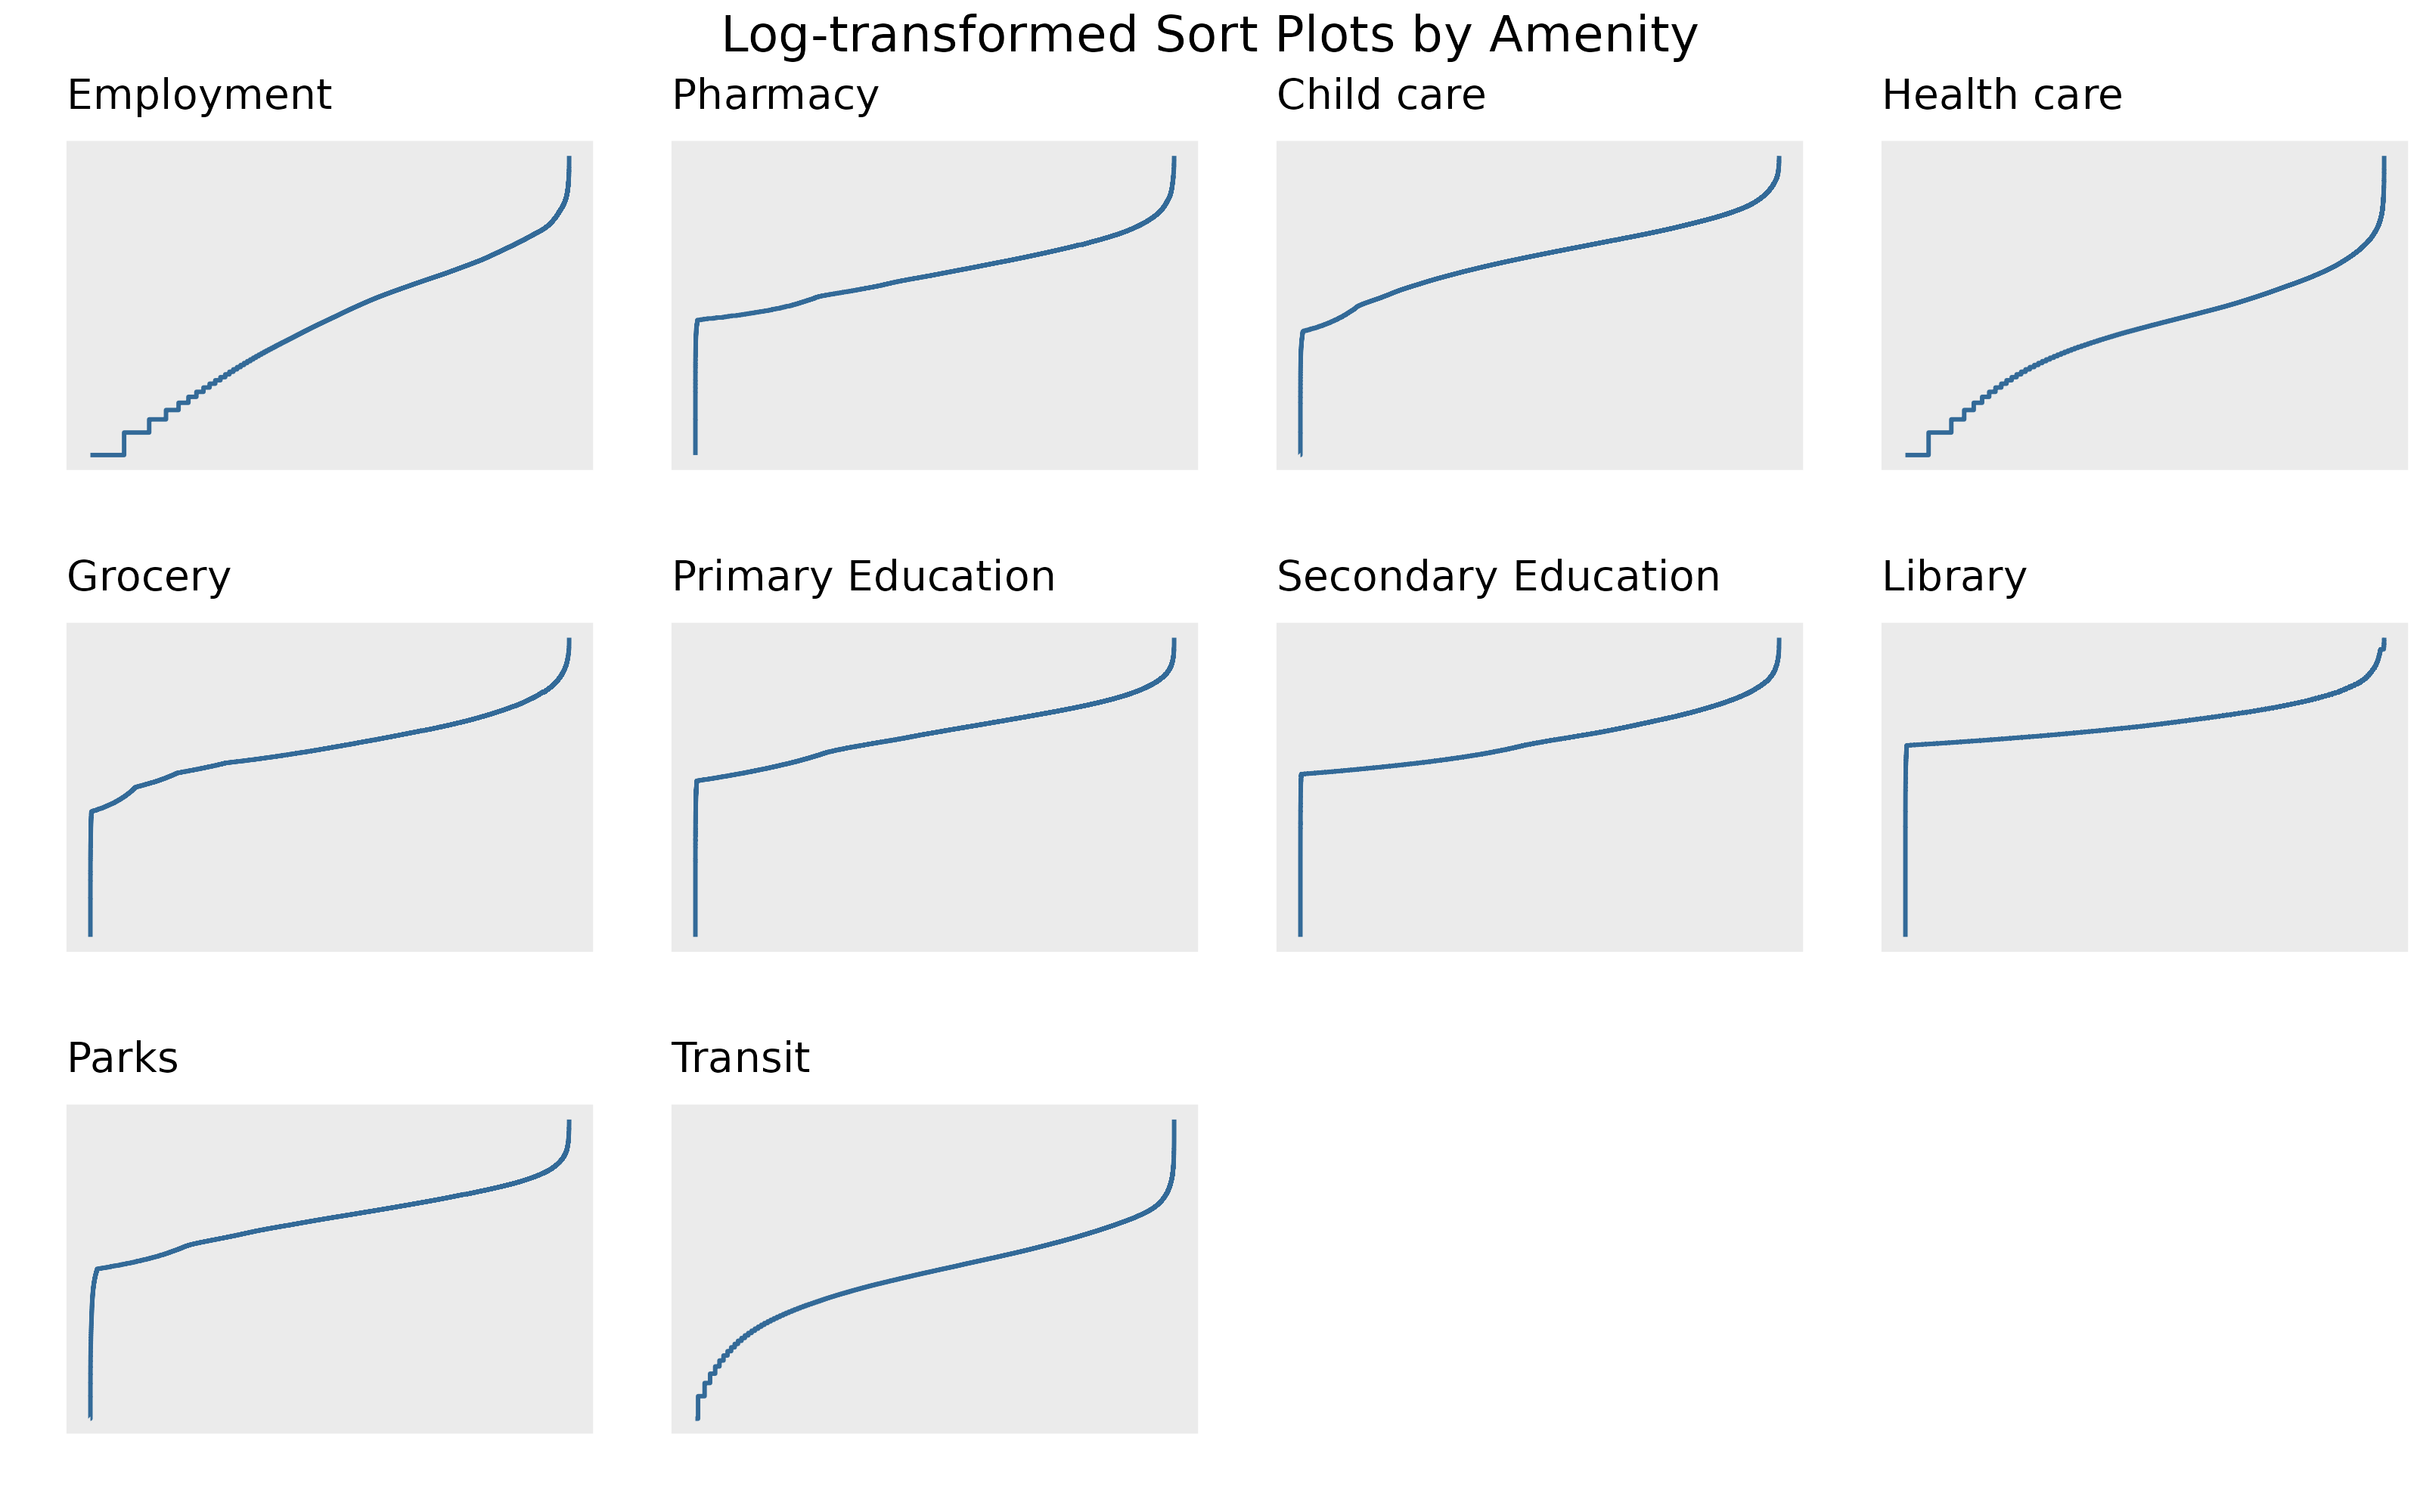
\includegraphics[width=\textwidth]{./sort_plot/log_sort_plot.png}
\caption[Log sort plots]{Log-transformed sort plots for each amenity in the PMD. 
}\label{logsortplots}
\end{figure}







\begin{figure}[H]
\centering
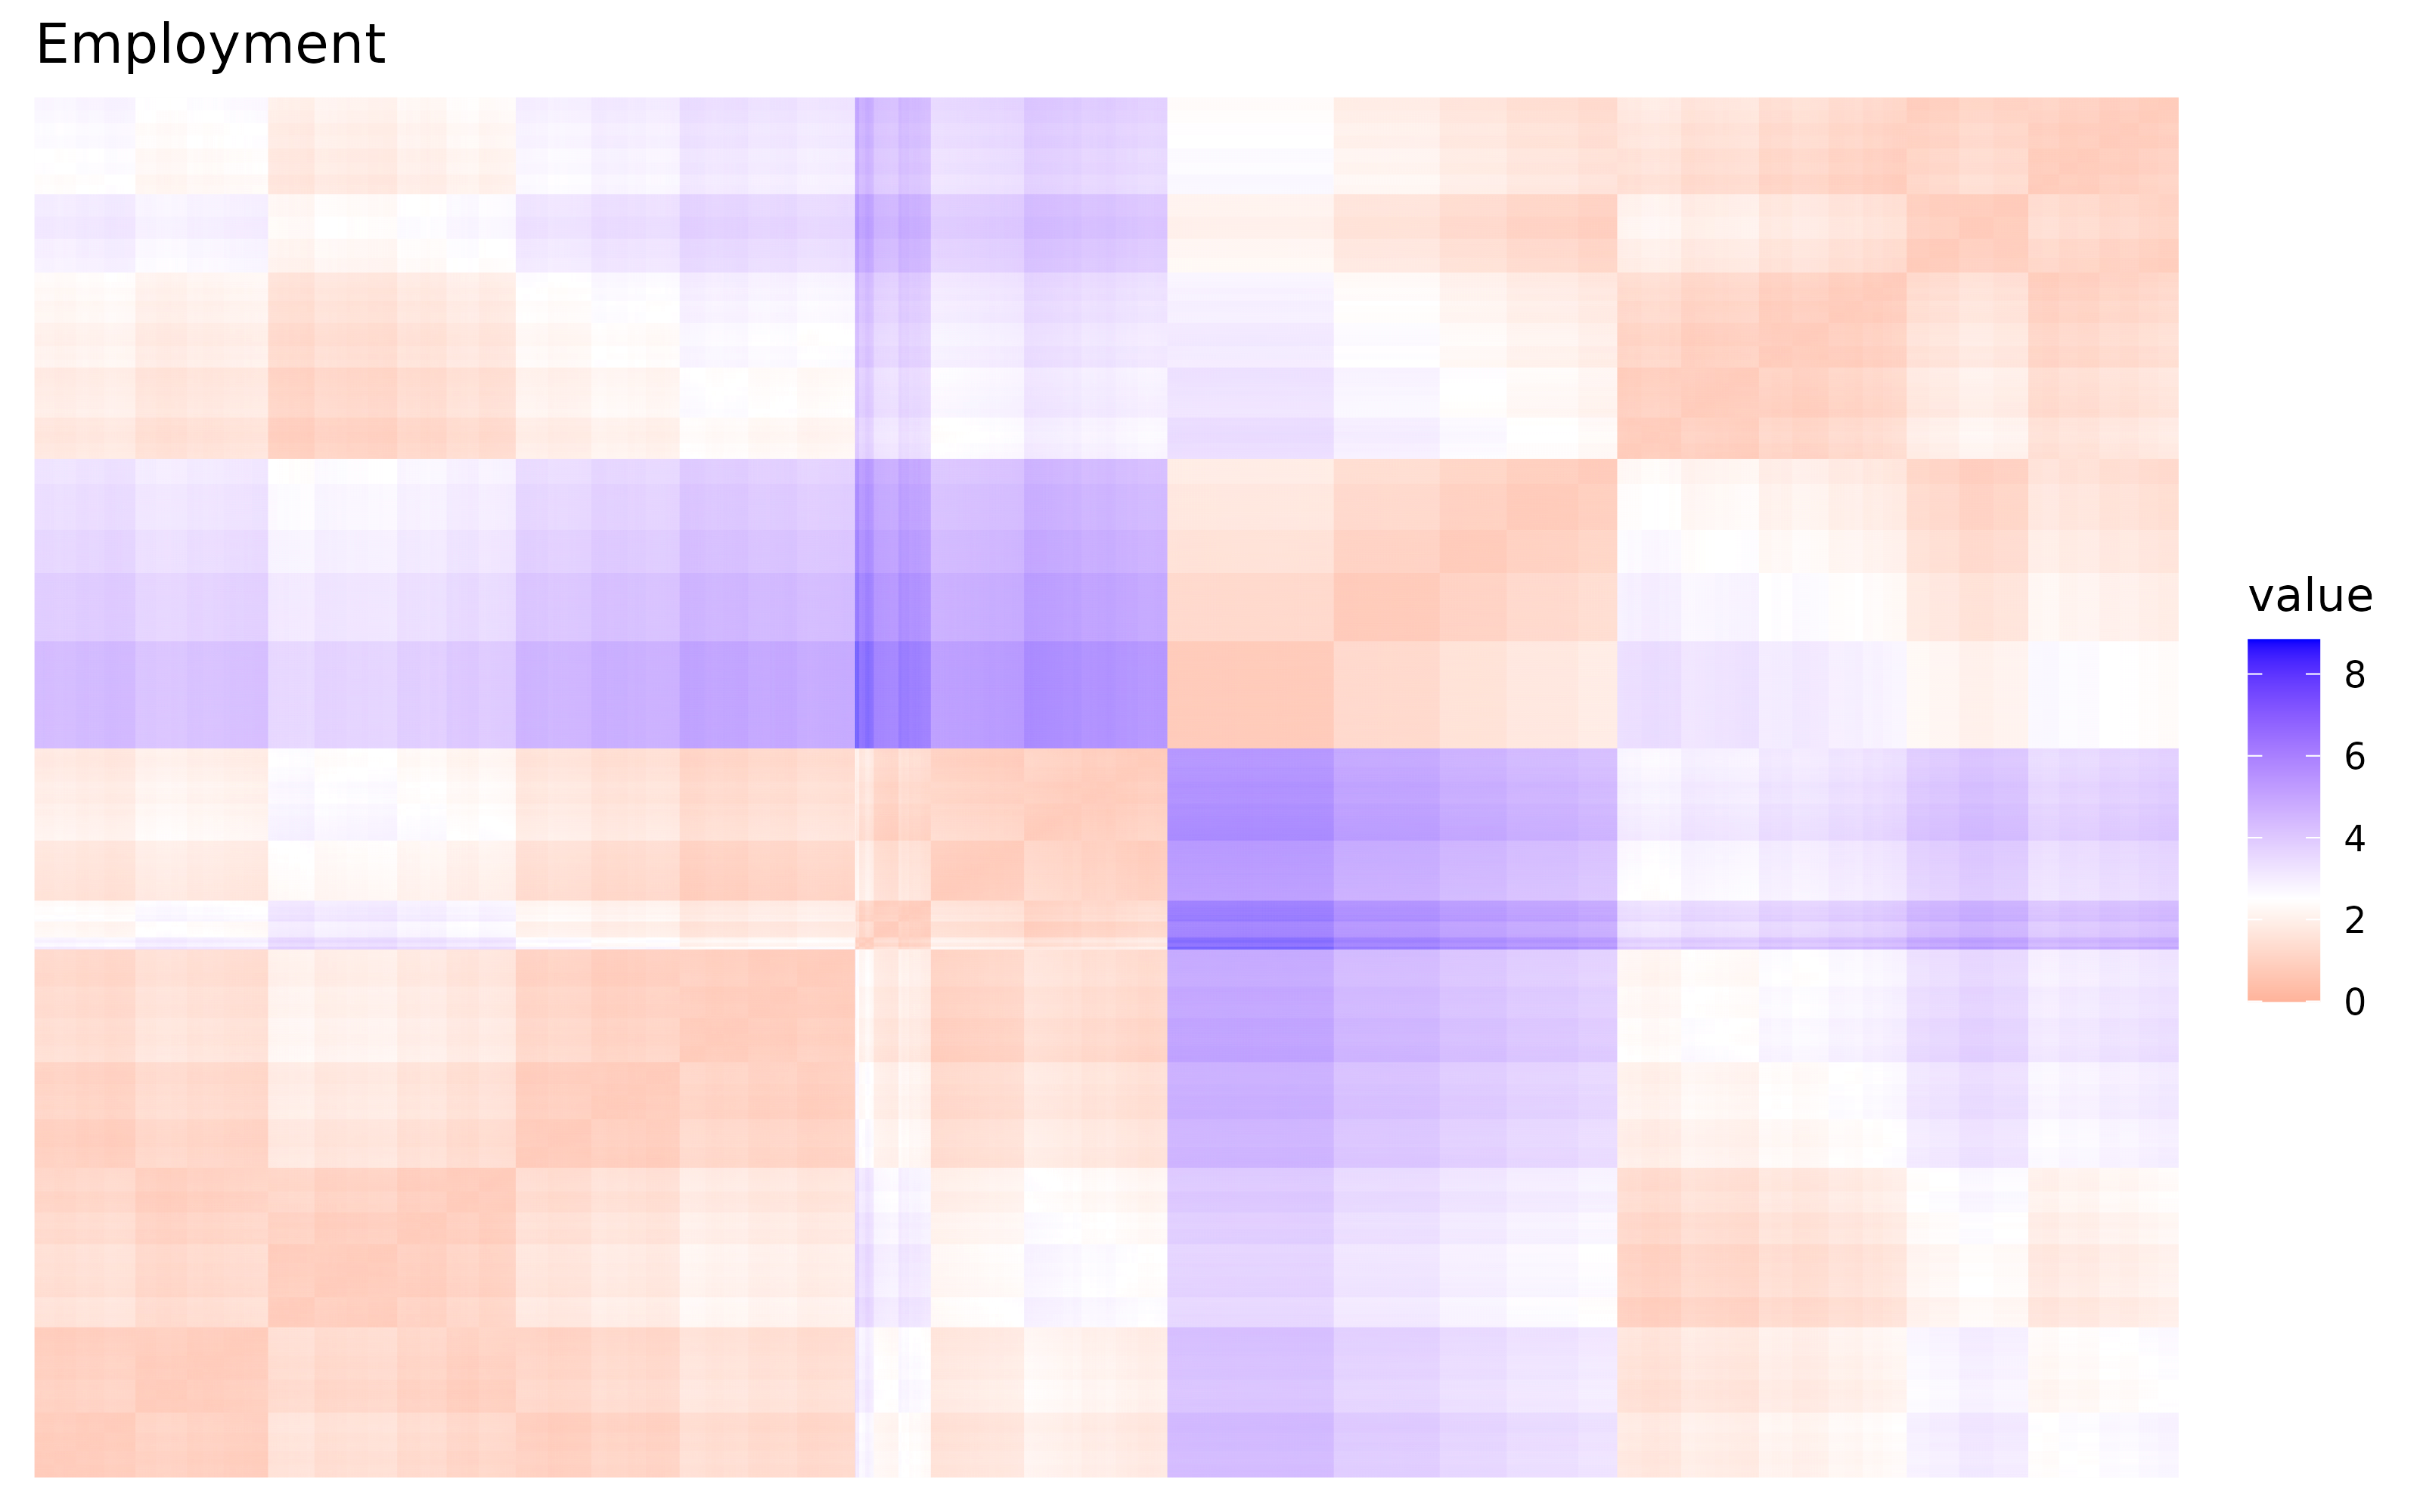
\includegraphics[width=\textwidth]{./vat/emp_vat_log.png}
\caption[Employment VAT plot]{VAT plot for the log-transformed employment amenity.}\label{empvat}
\end{figure}








\begin{figure}[H]
\centering
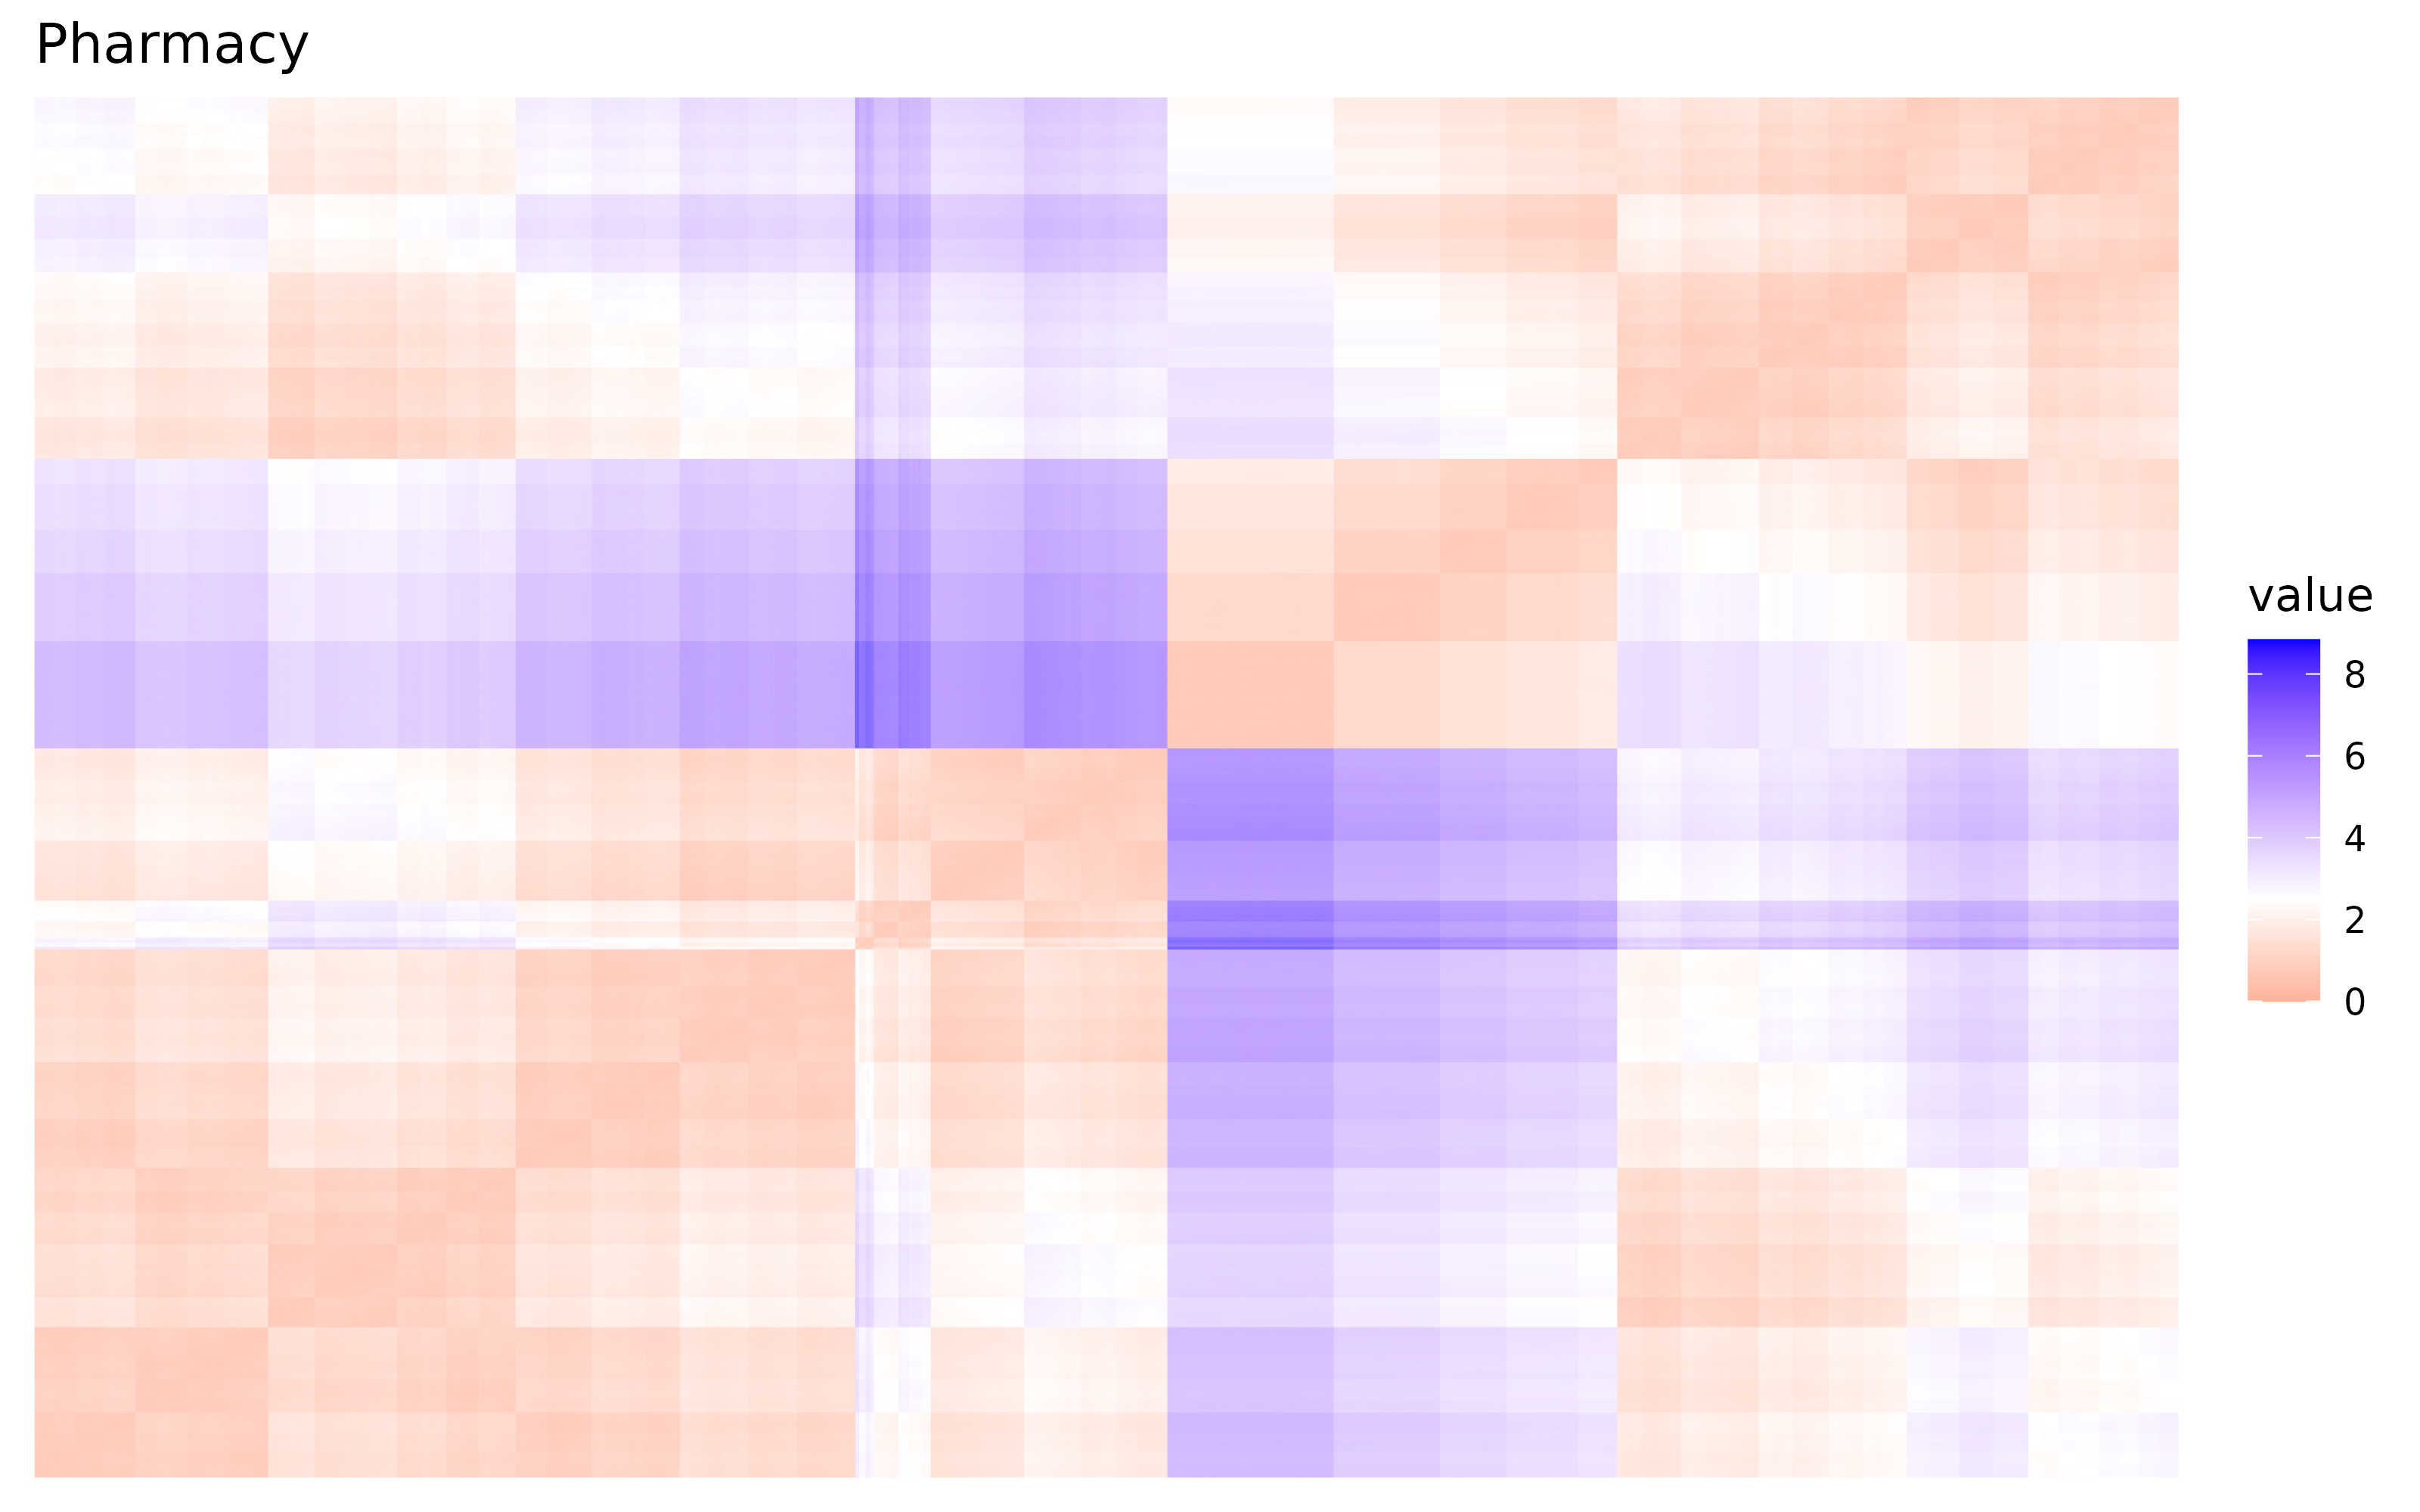
\includegraphics[width=\textwidth]{./vat/pharma_vat_log.png}
\caption[Pharmacy VAT plot]{VAT plot for the log-transformed pharmacy amenity.}\label{pharmavat}
\end{figure}






\begin{figure}[H]
\centering
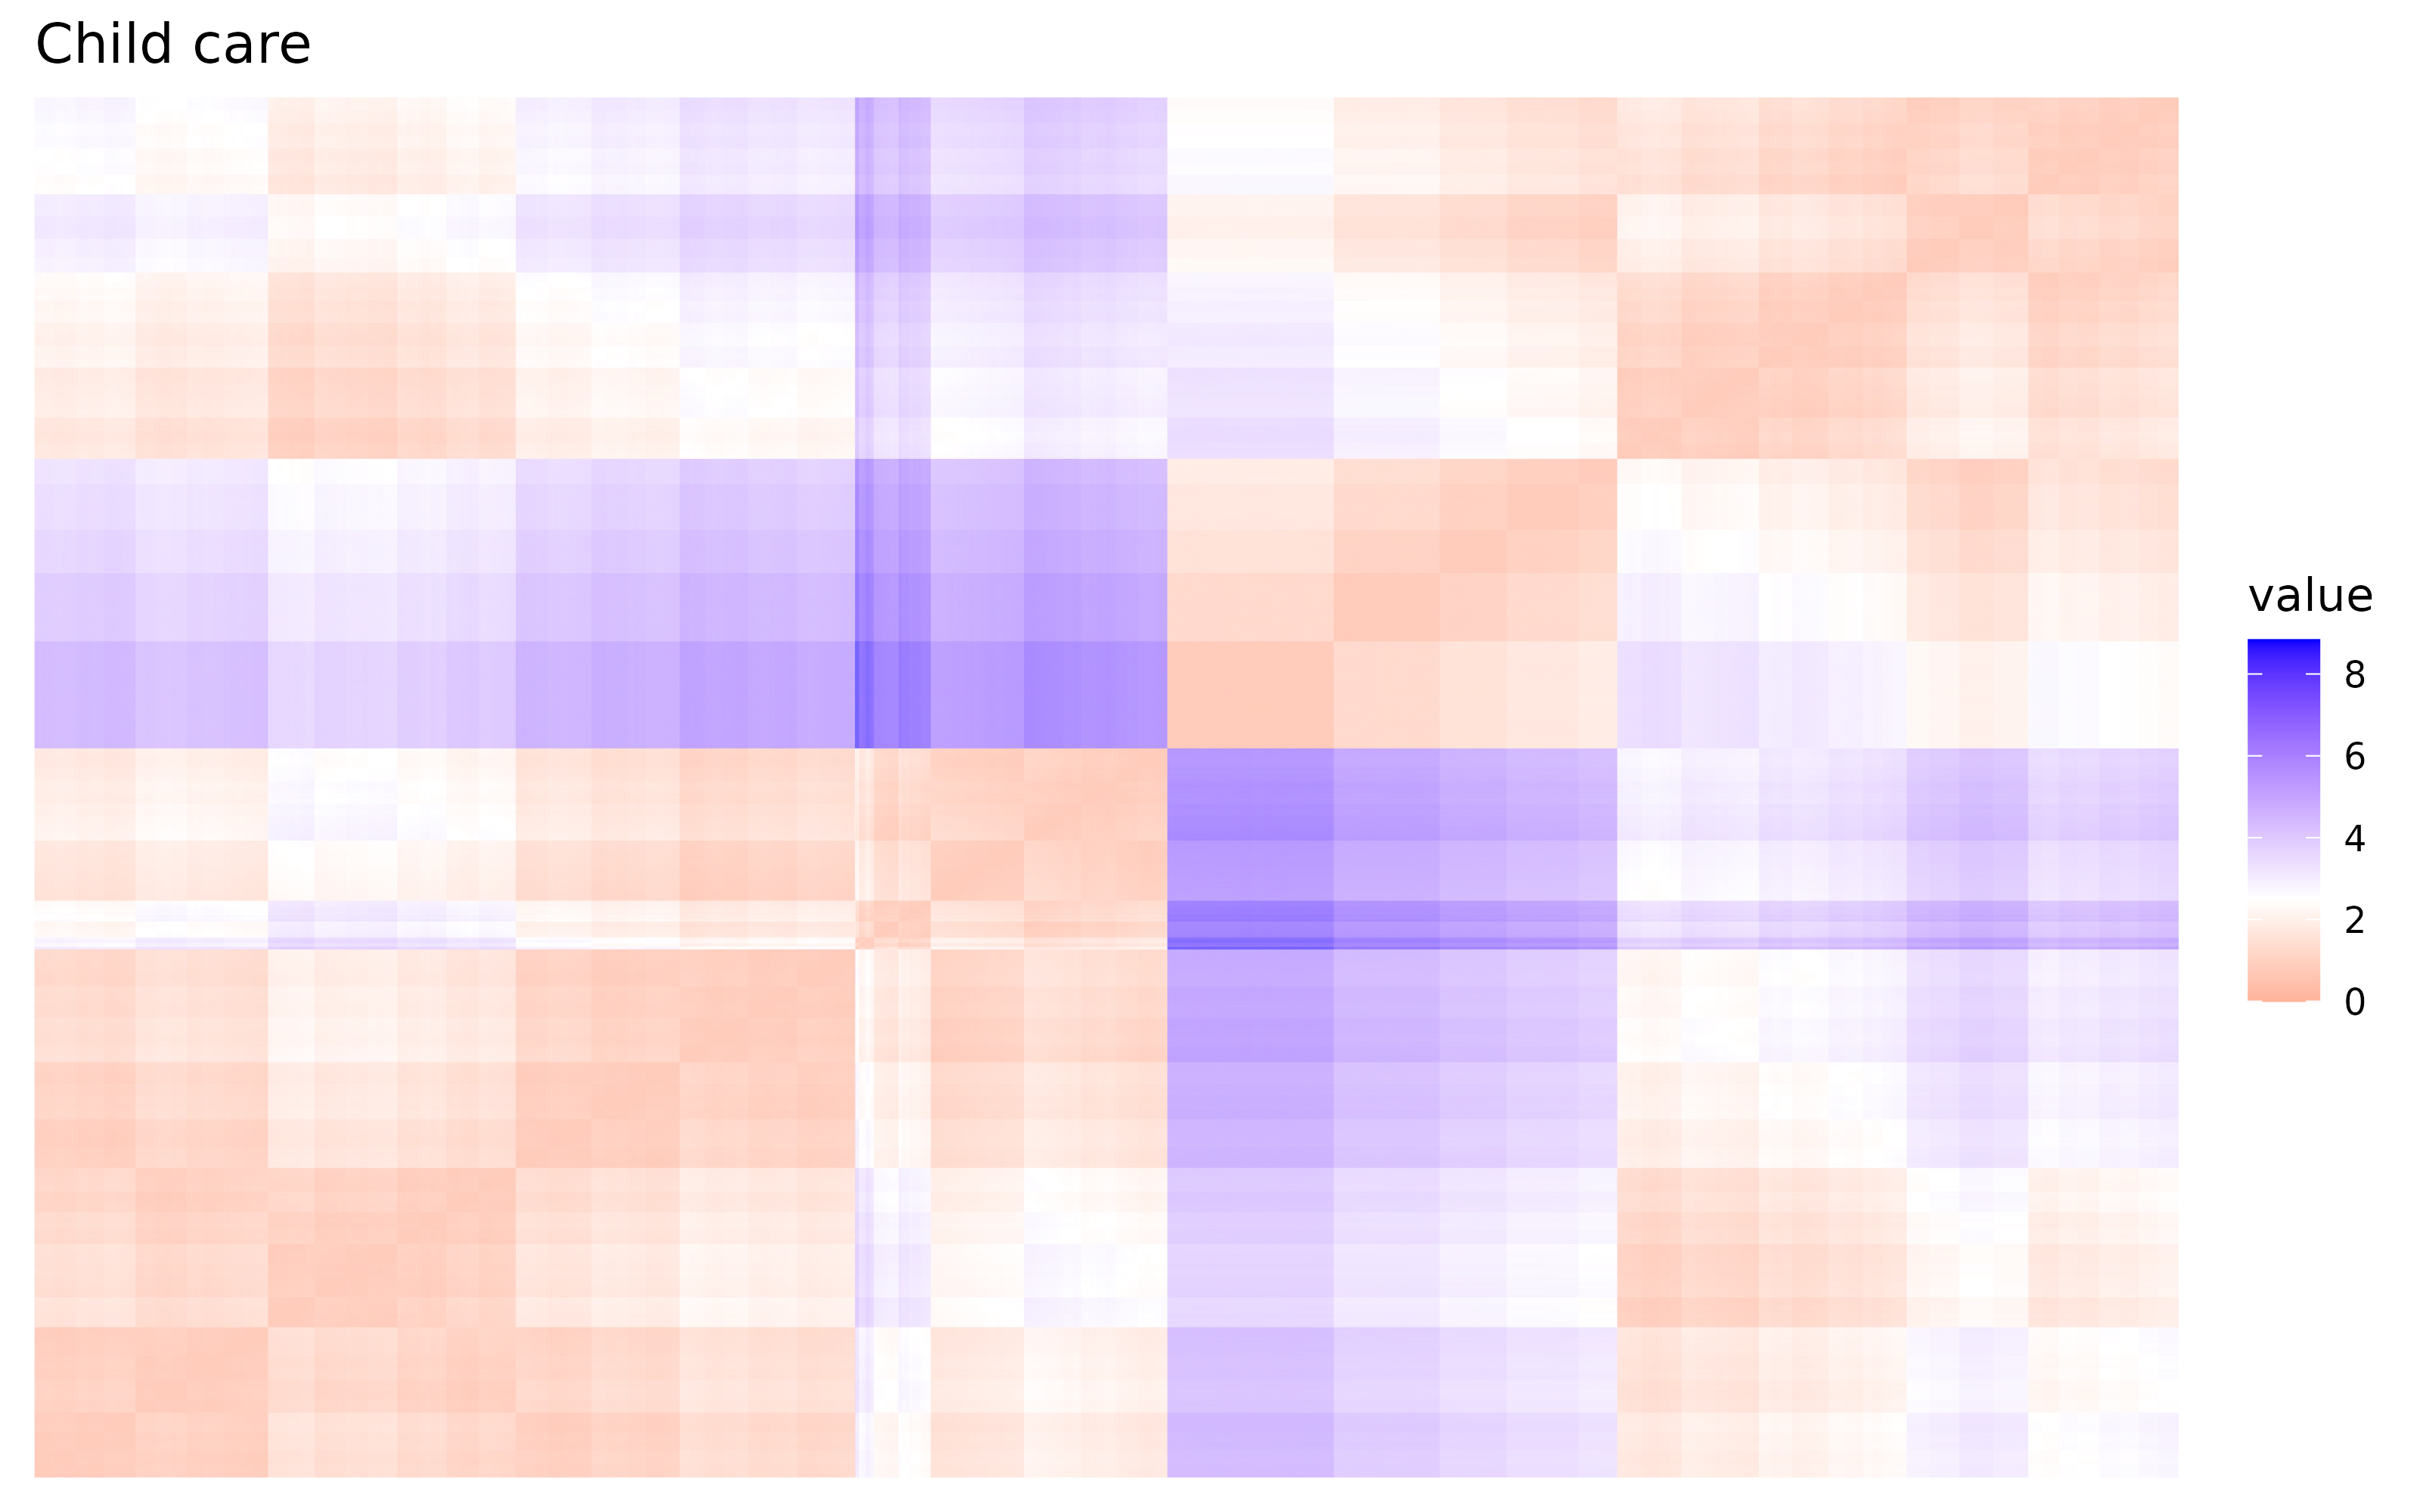
\includegraphics[width=\textwidth]{./vat/childcare_vat_log.png}
\caption[Child care VAT plot]{VAT plot for the log-transformed child care amenity.}\label{childcarevat}
\end{figure}








\begin{figure}[H]
\centering
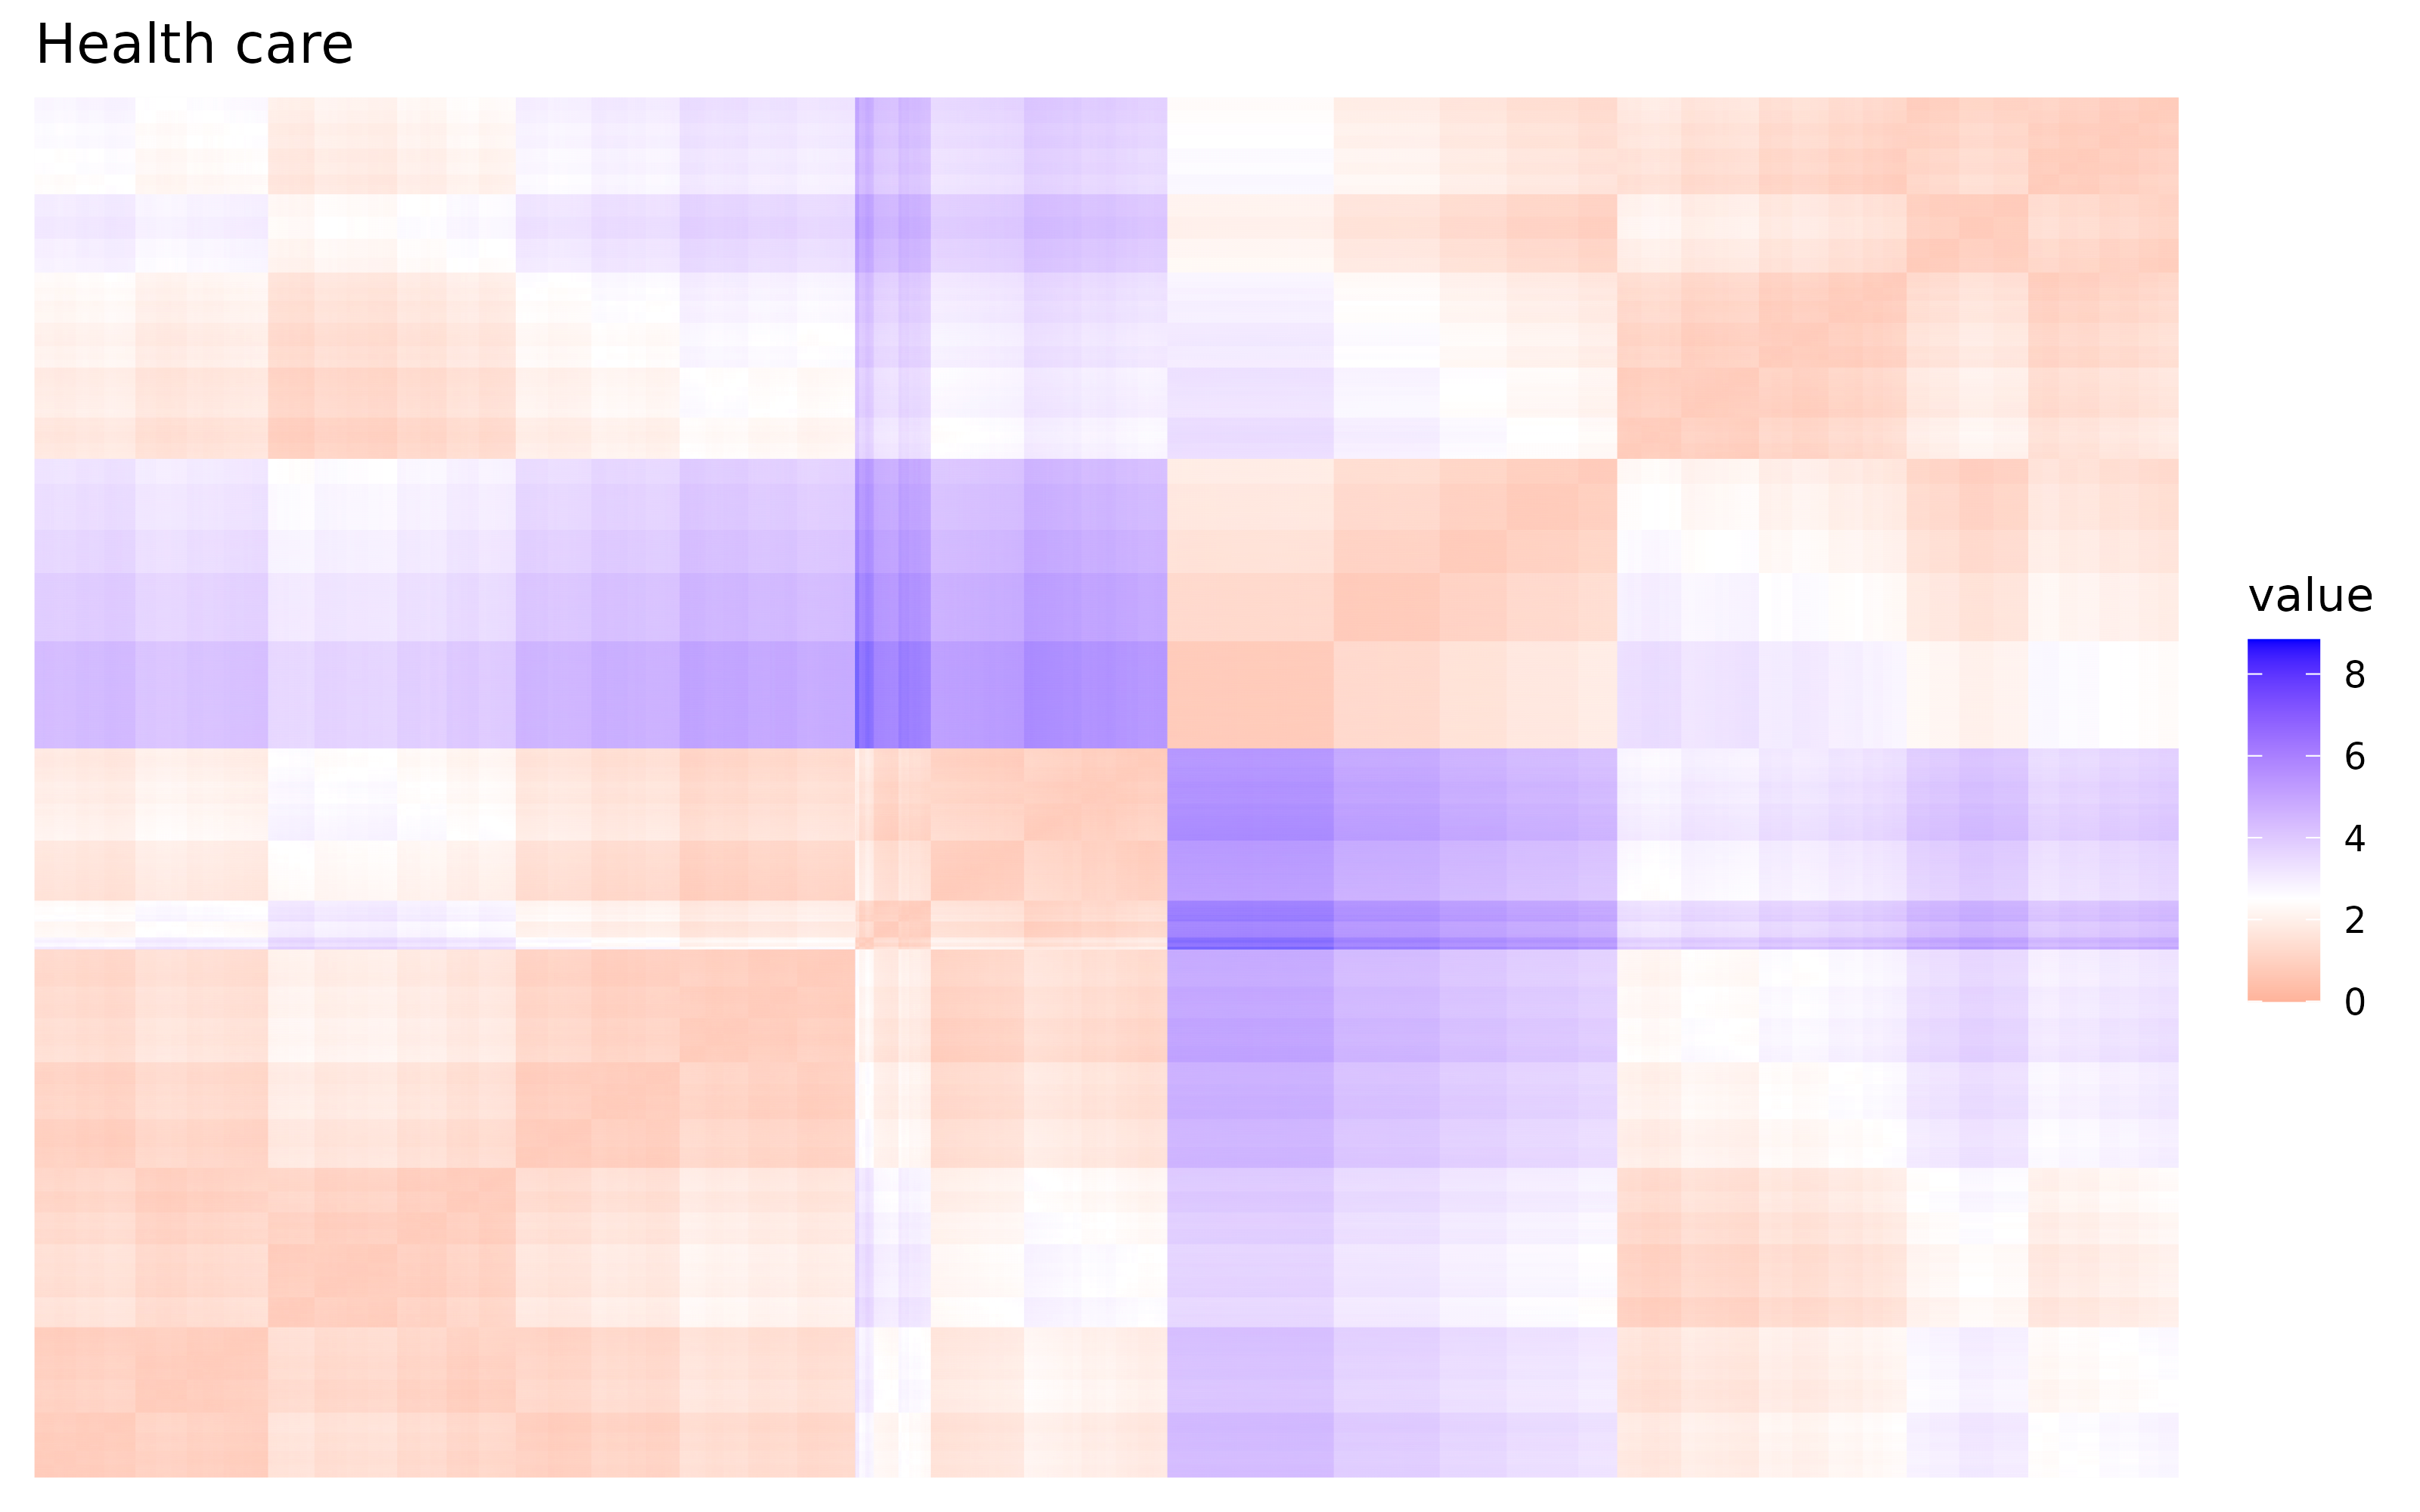
\includegraphics[width=\textwidth]{./vat/healthcare_vat_log.png}
\caption[Health care VAT plot]{VAT plot for the log-transformed health care amenity.}\label{healthcarevat}
\end{figure}







\begin{figure}[H]
\centering
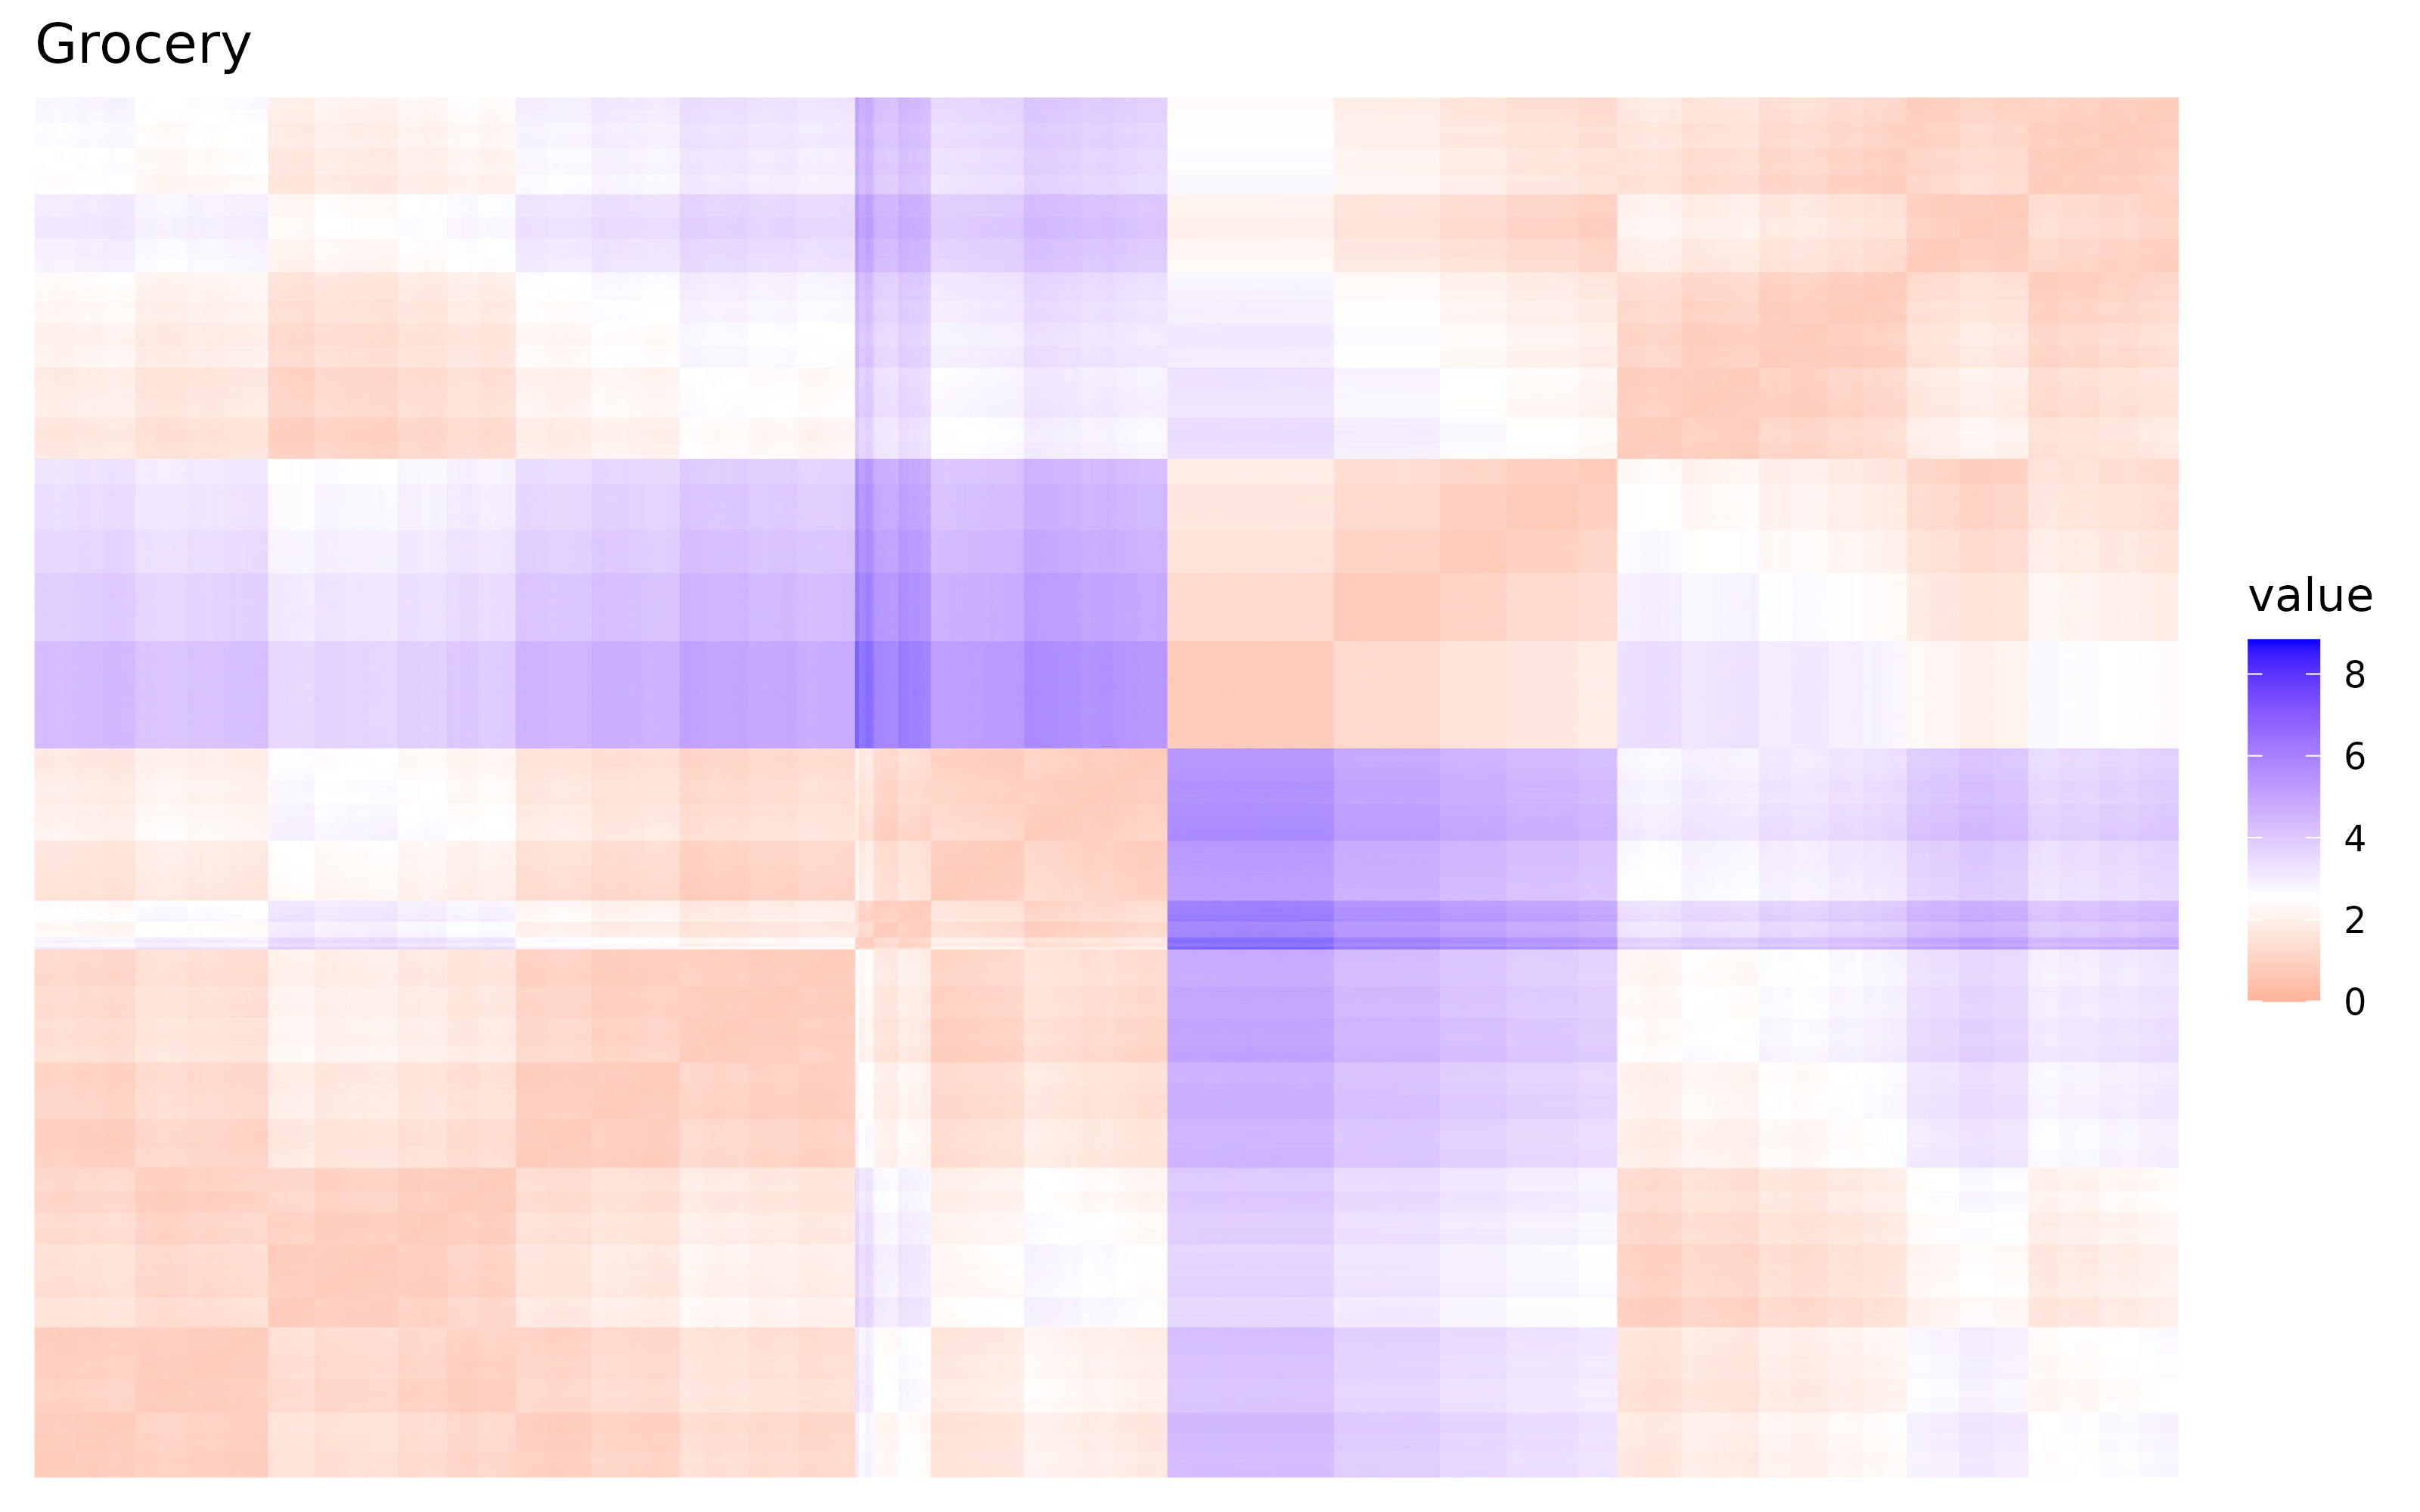
\includegraphics[width=\textwidth]{./vat/grocery_vat_log.png}
\caption[Grocery VAT plot]{VAT plot for the log-transformed grocery amenity.}\label{groceryvat}
\end{figure}








\begin{figure}[H]
\centering
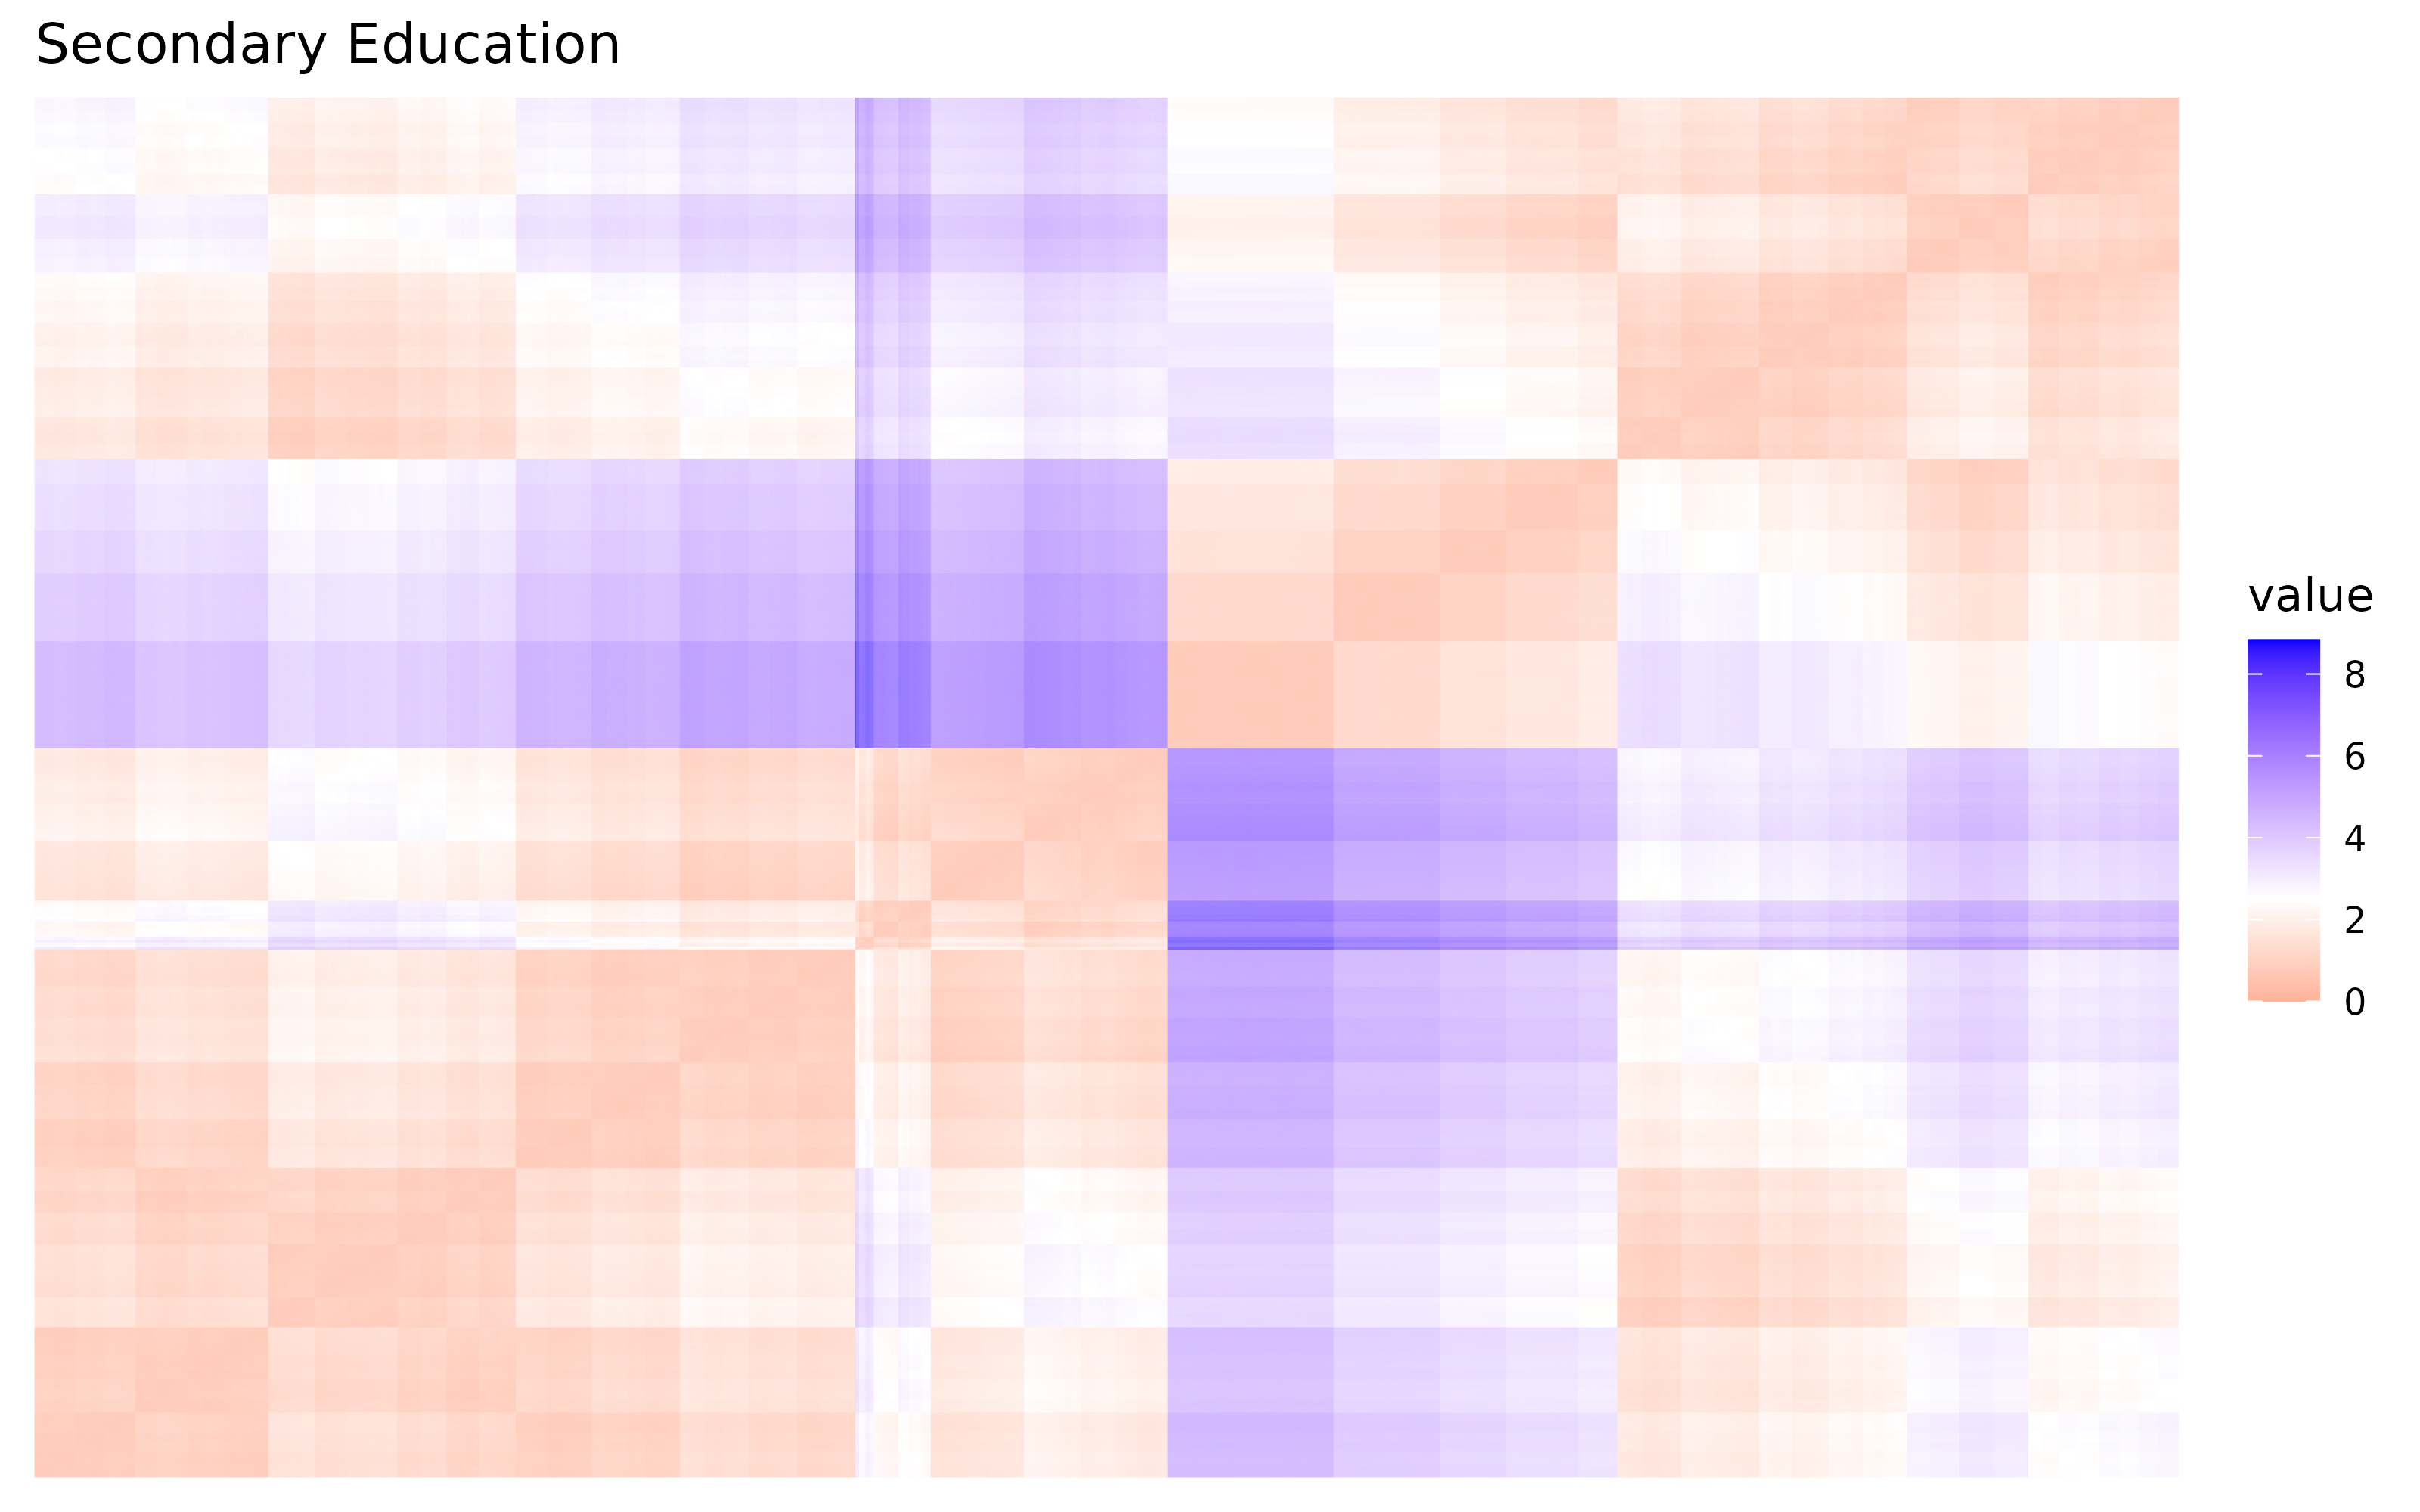
\includegraphics[width=\textwidth]{./vat/secondaryeducation_vat_log.png}
\caption[Secondary education VAT plot]{VAT plot for the log-transformed secondary education amenity.}\label{seceducvat}
\end{figure}








\begin{figure}[H]
\centering
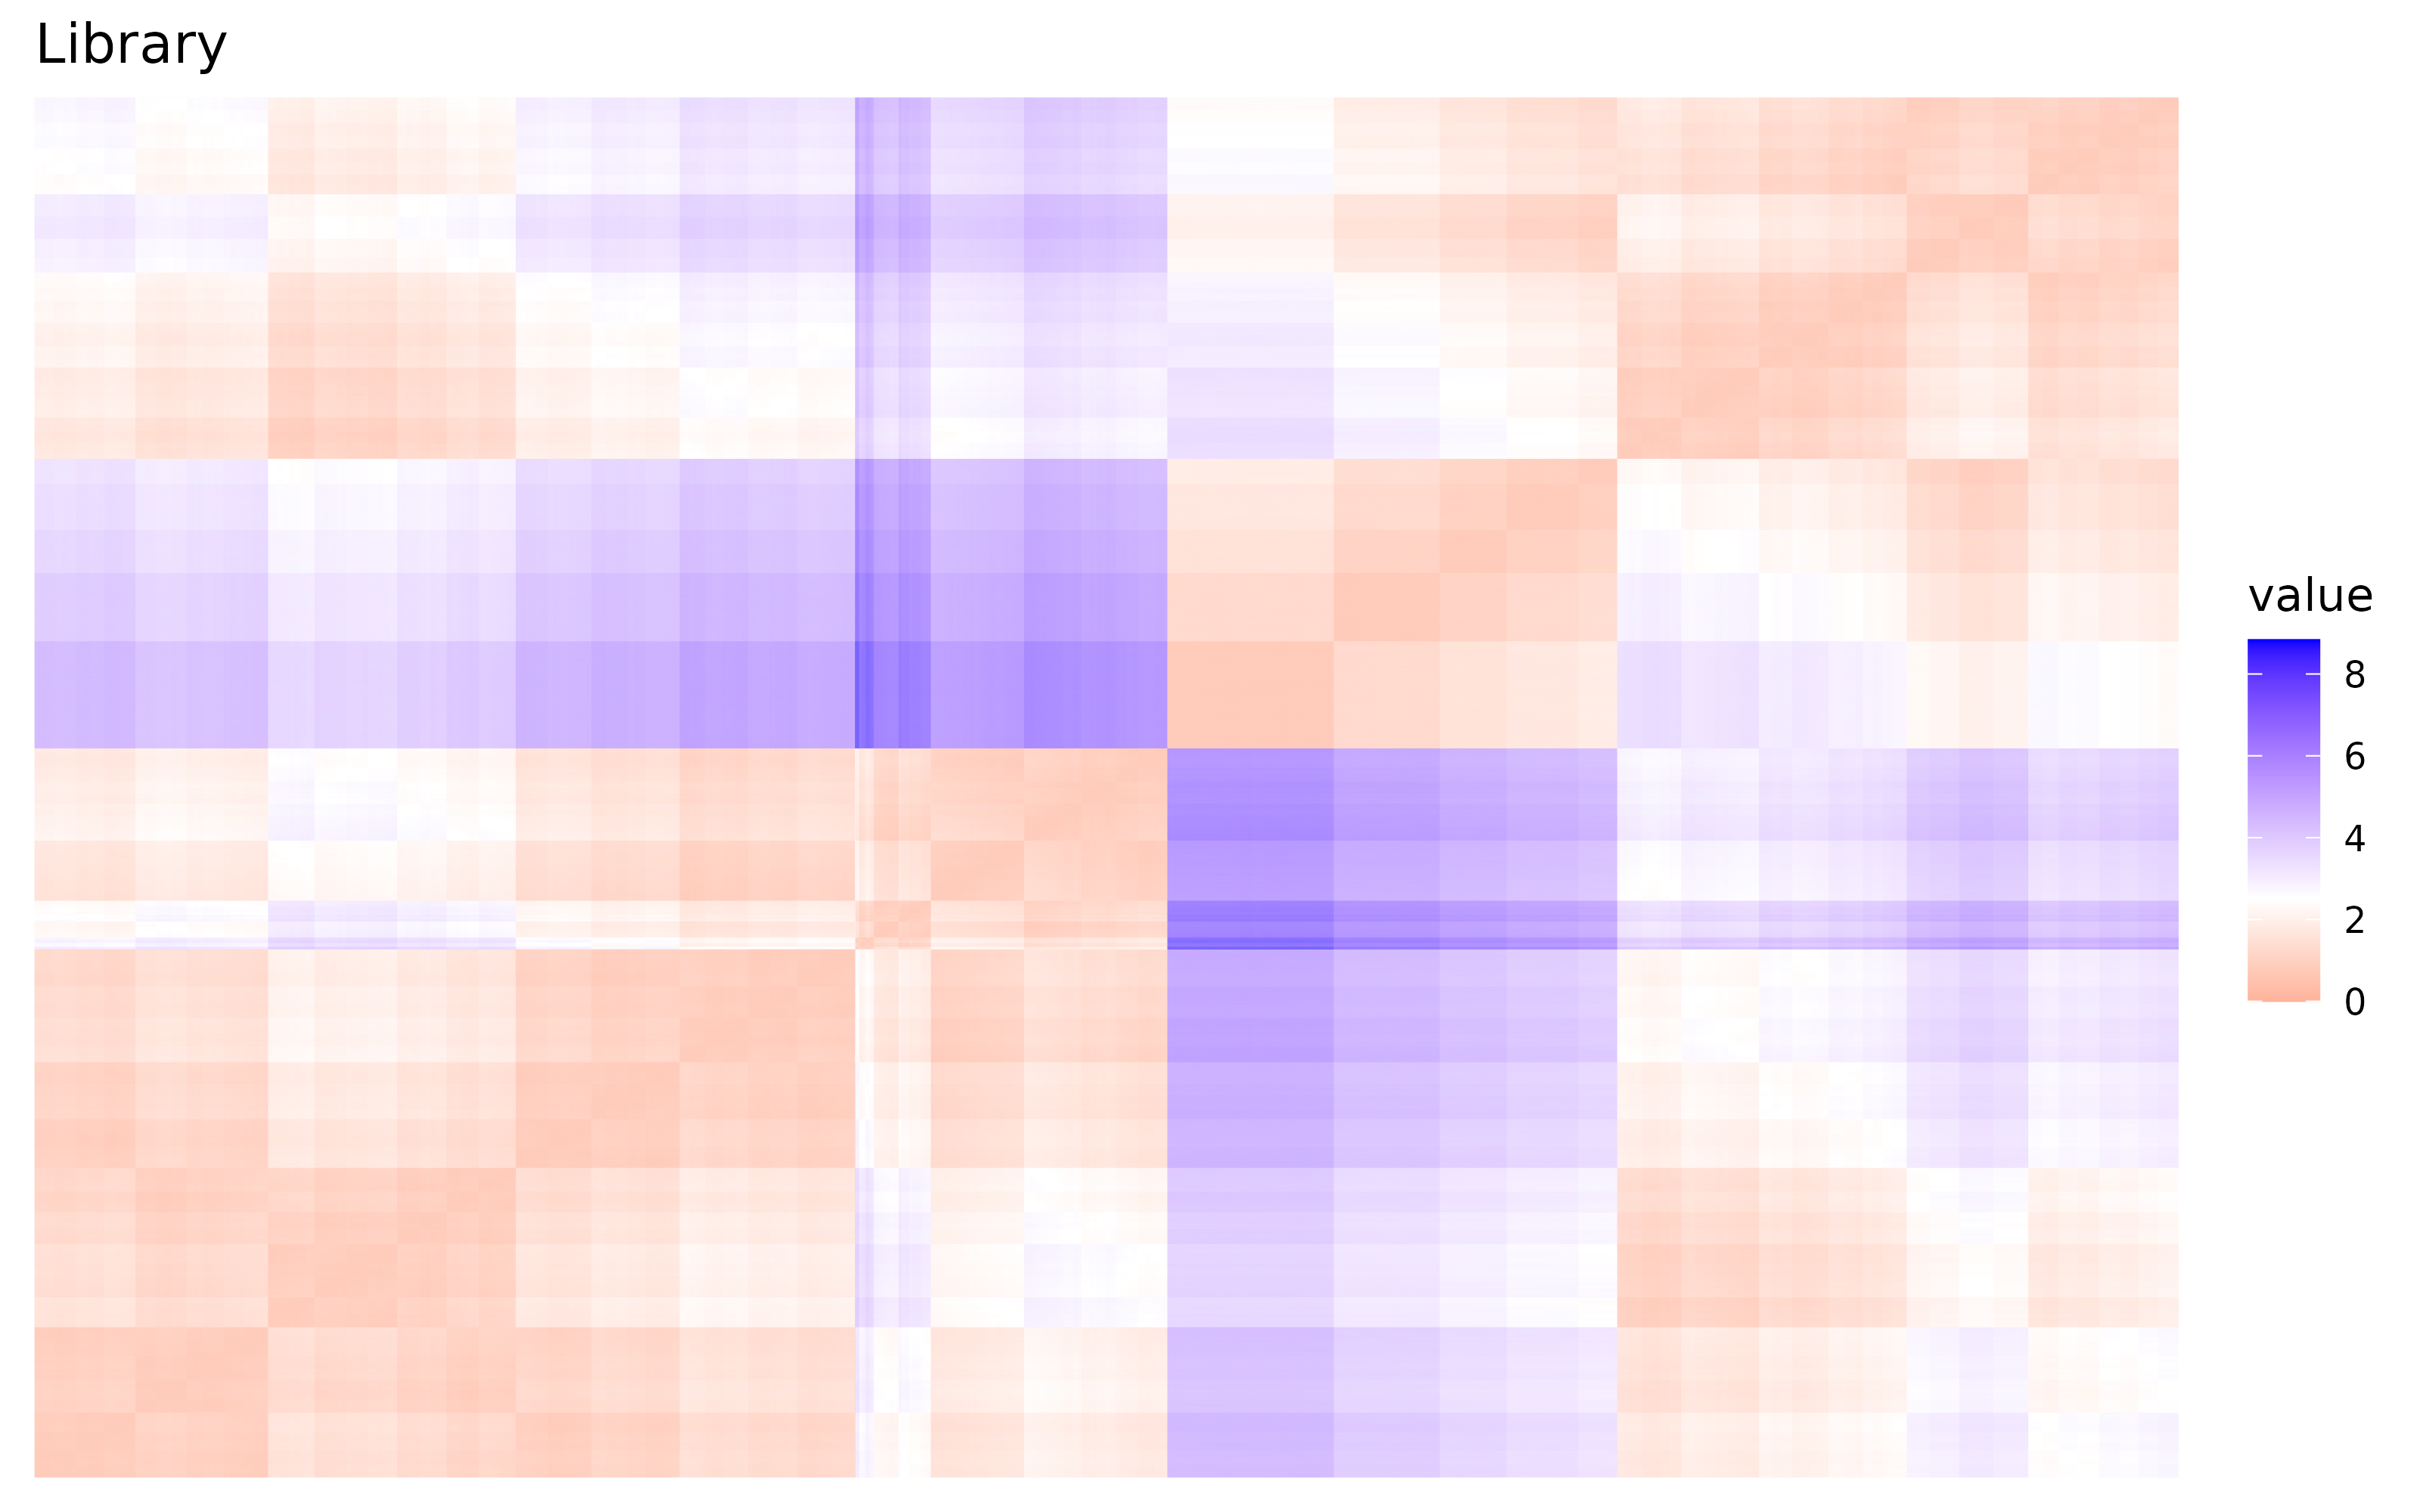
\includegraphics[width=\textwidth]{./vat/library_vat_log.png}
\caption[Library VAT plot]{VAT plot for the log-transformed library amenity.}\label{libraryvat}
\end{figure}








\begin{figure}[H]
\centering
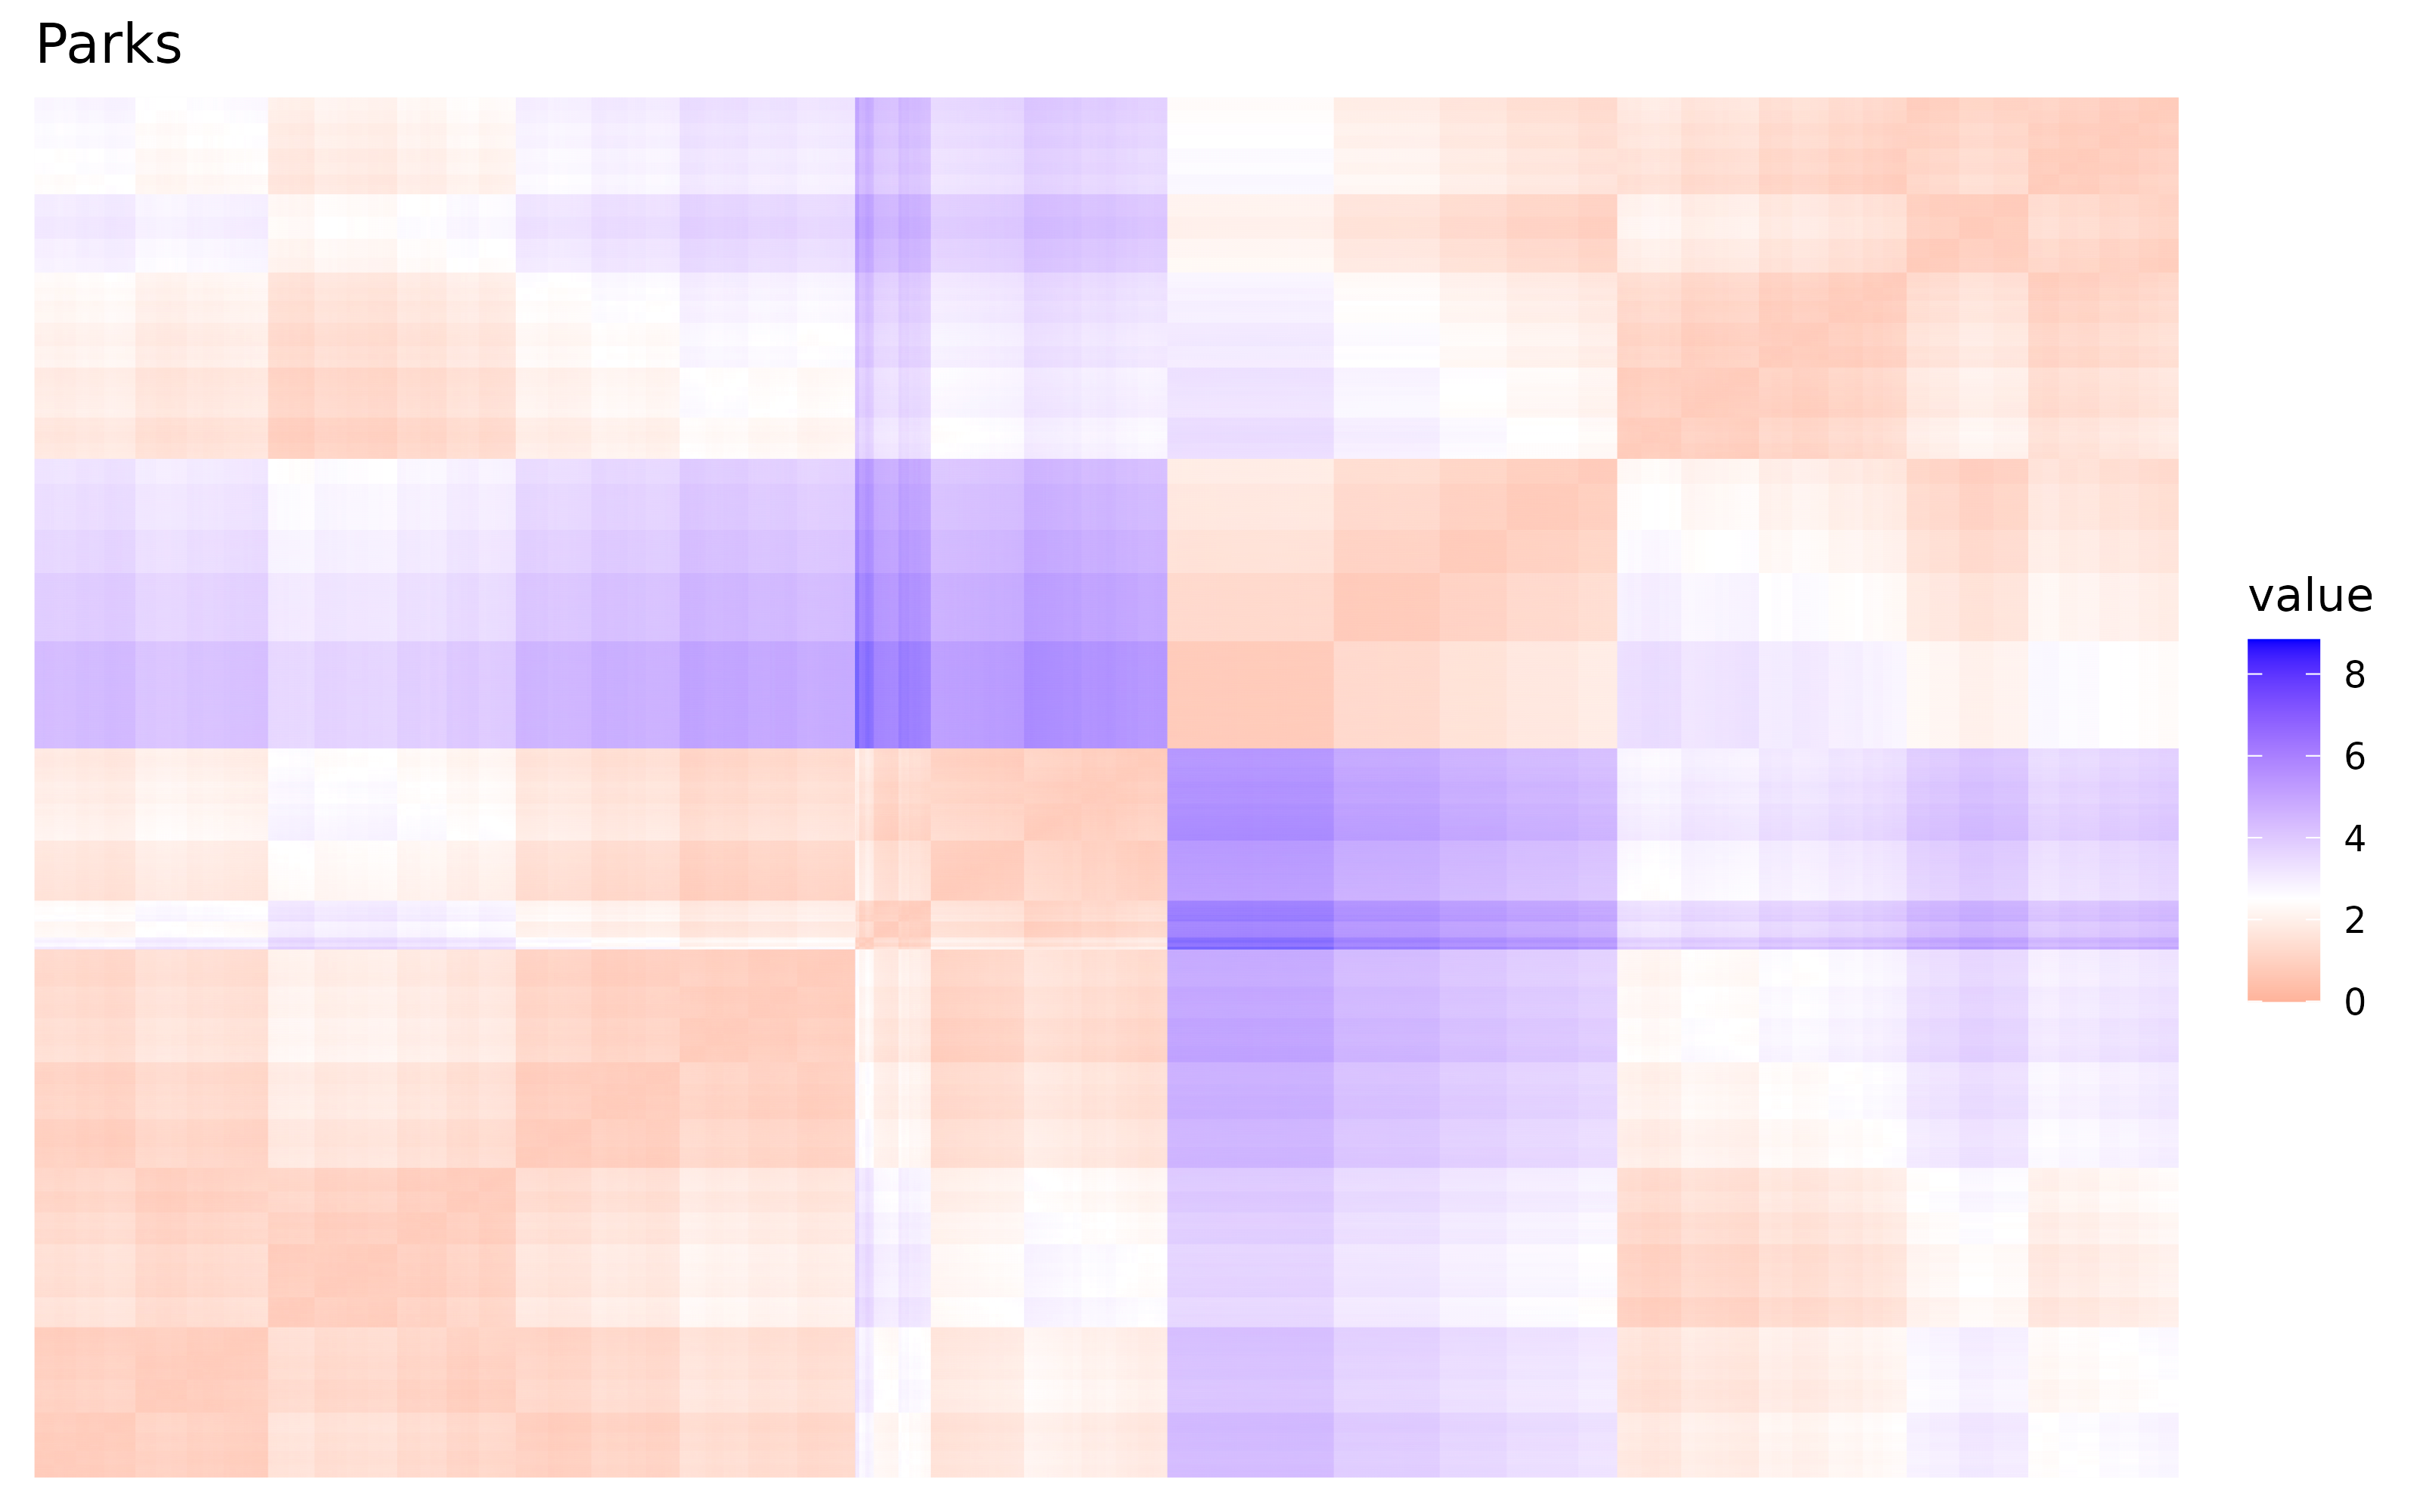
\includegraphics[width=\textwidth]{./vat/parks_vat_log.png}
\caption[Parks VAT plot]{VAT plot for the log-transformed parks amenity.}\label{parksvat}
\end{figure}










\begin{figure}[H]
\centering
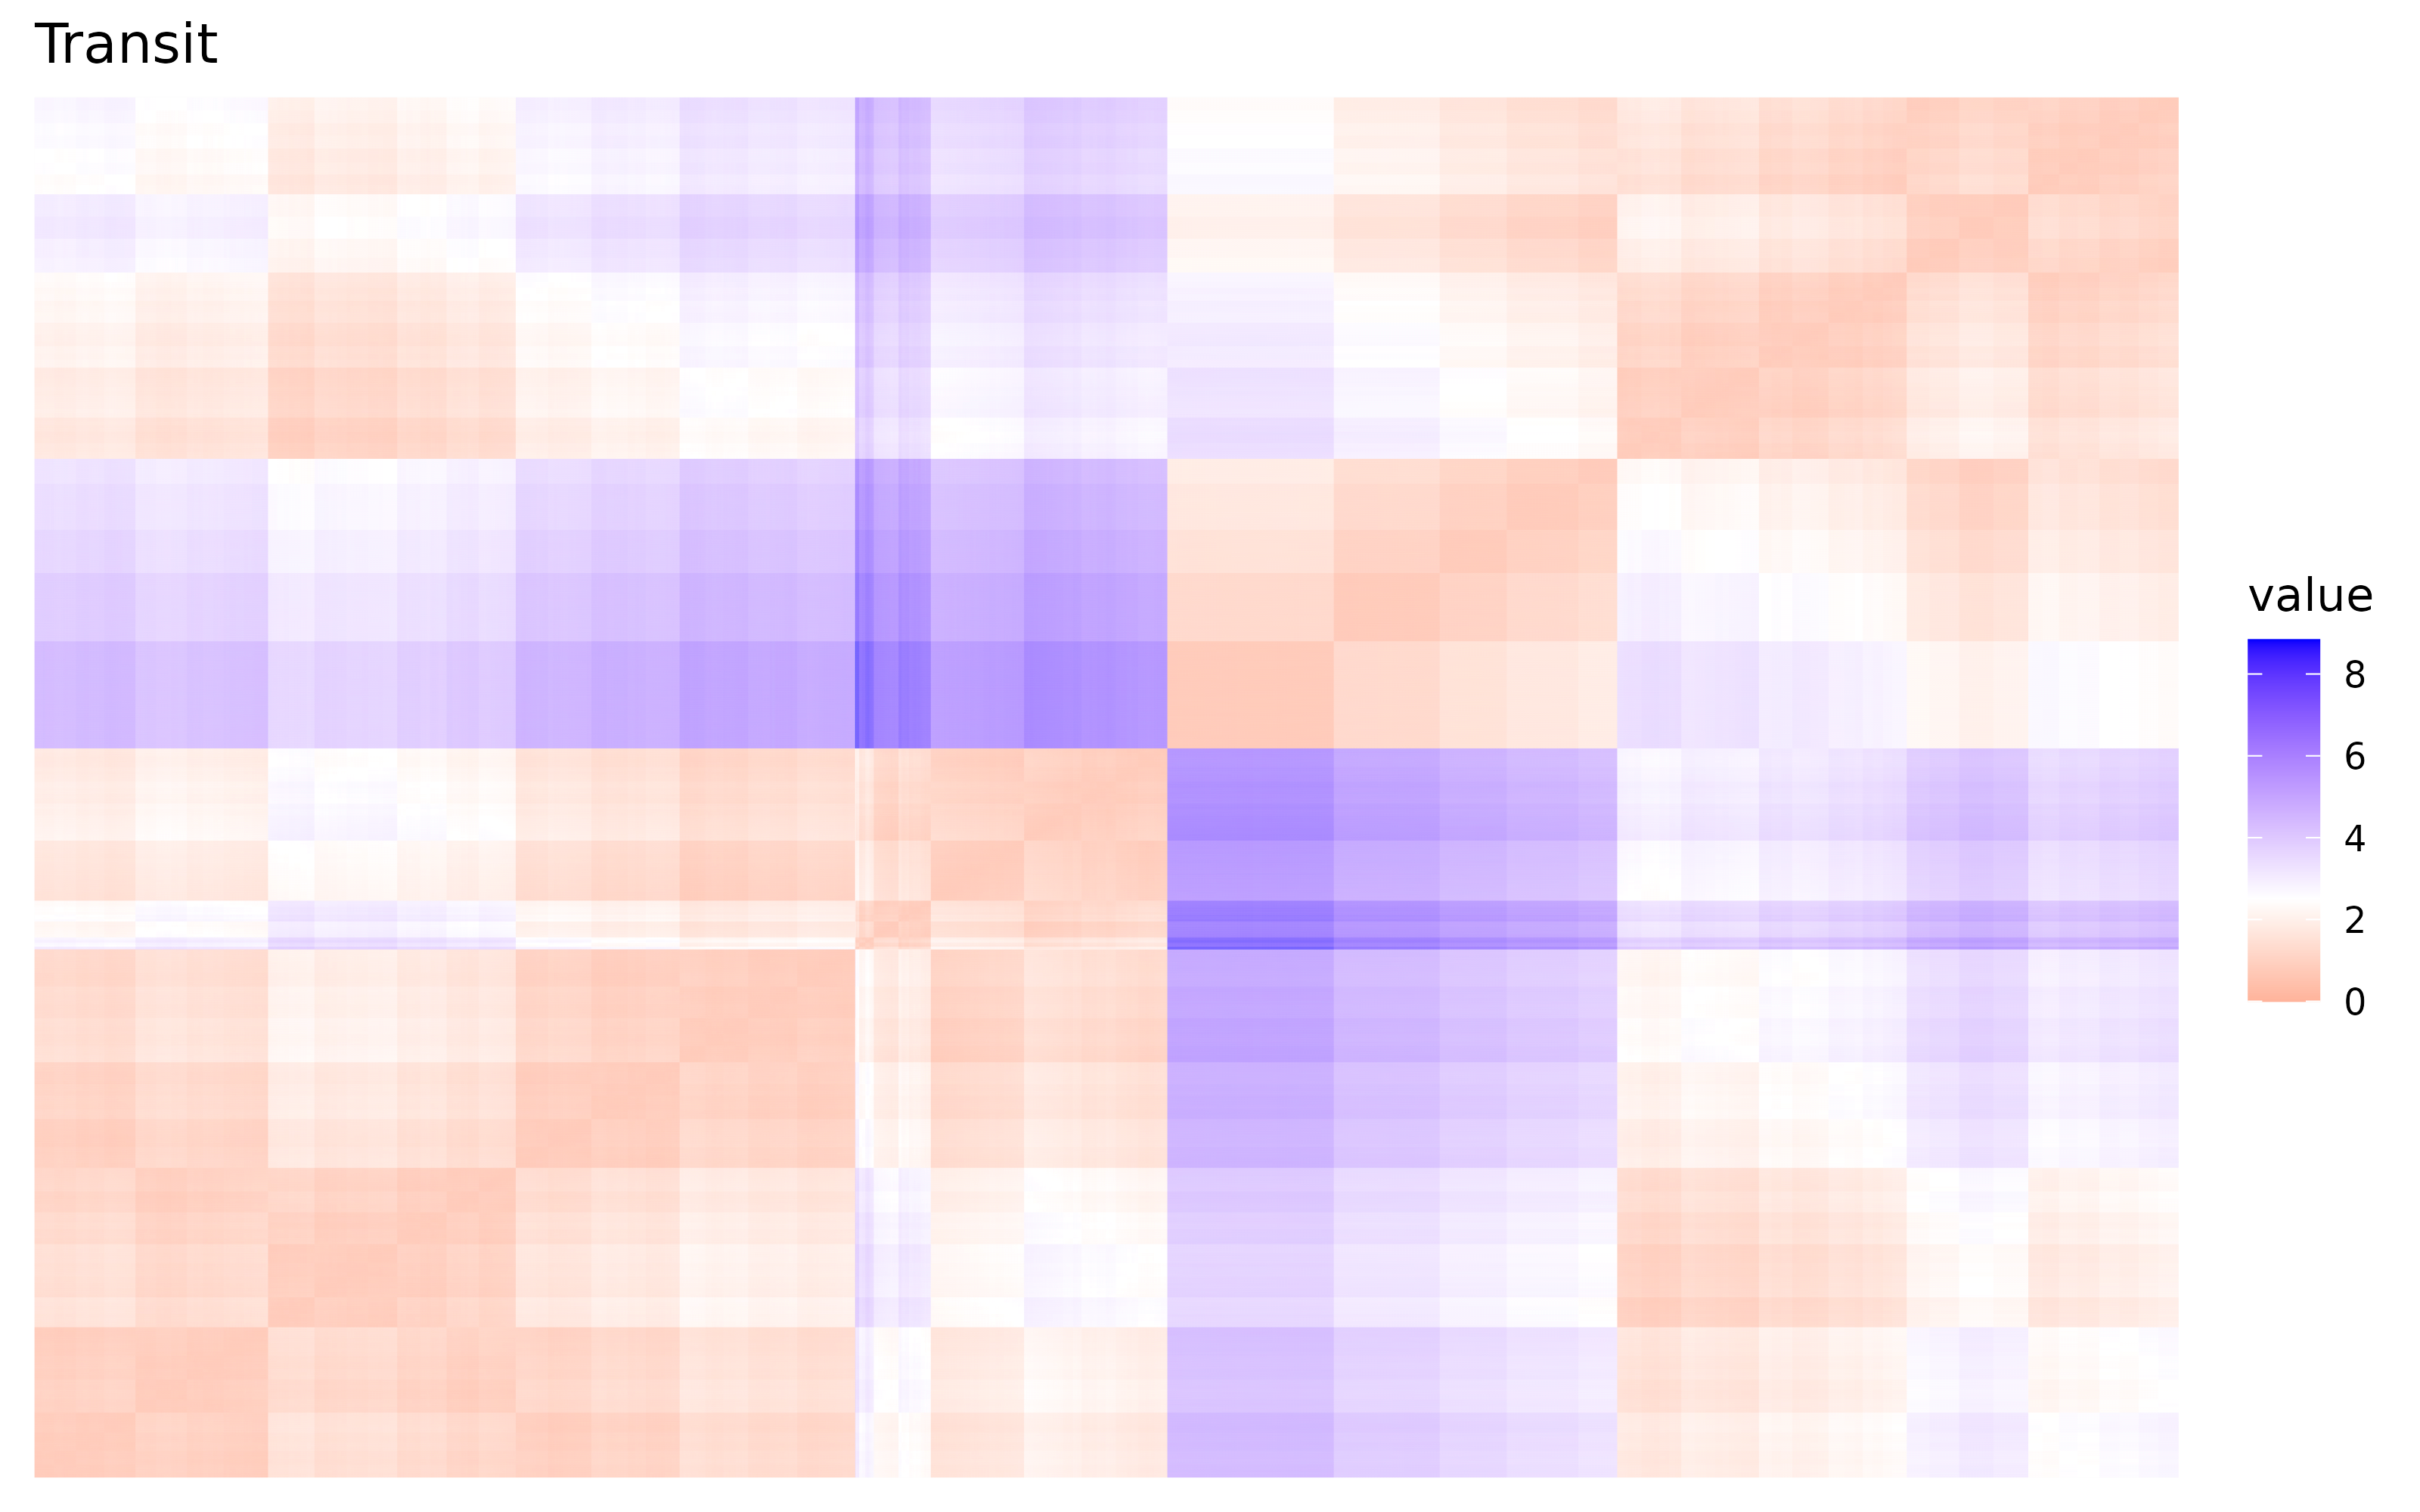
\includegraphics[width=\textwidth]{./vat/transit_vat_log.png}
\caption[Transit VAT plot]{VAT plot for the log-transformed transit amenity.}\label{transitvat}
\end{figure}









\begin{figure}[H]
\centering
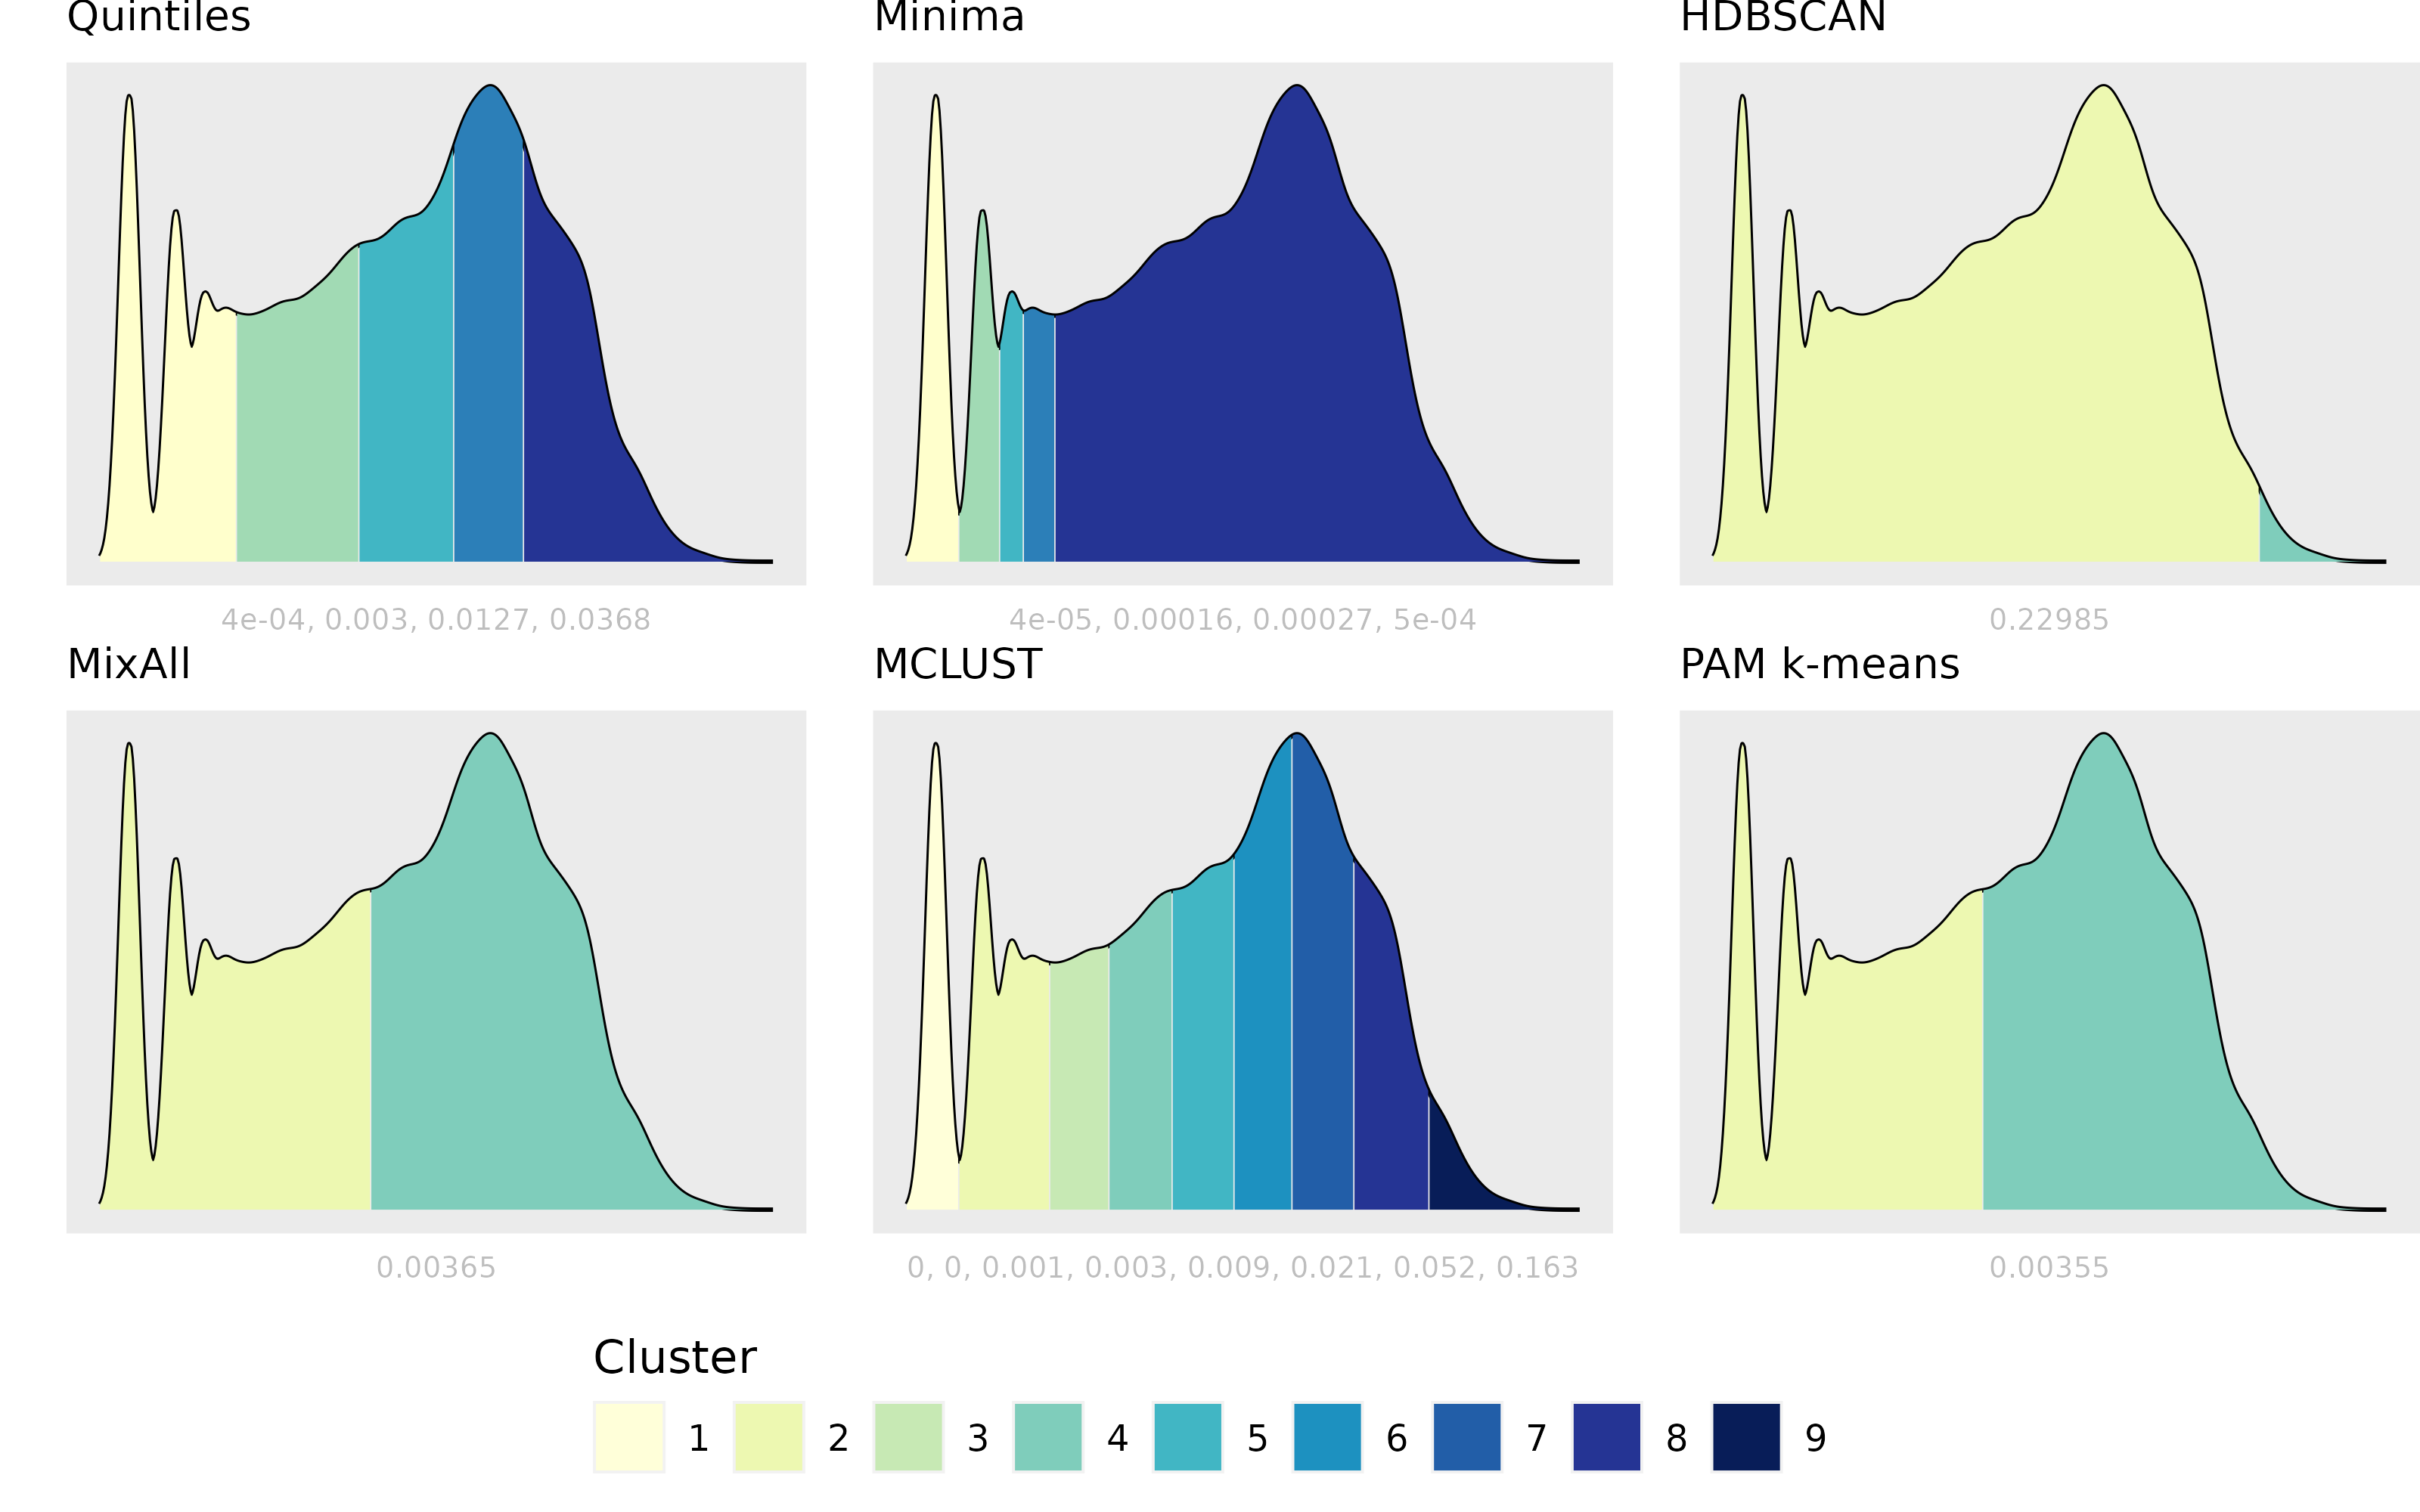
\includegraphics[width=\textwidth]{./cutoffs/by_amenity/Employment_cutoffs.png}
\caption[Employment cutoffs]{Cut-offs values shown on the log-transformed density plots for all clustering approaches employment amenity.}\label{employmentcutoffs}
\end{figure}









\begin{figure}[H]
\centering
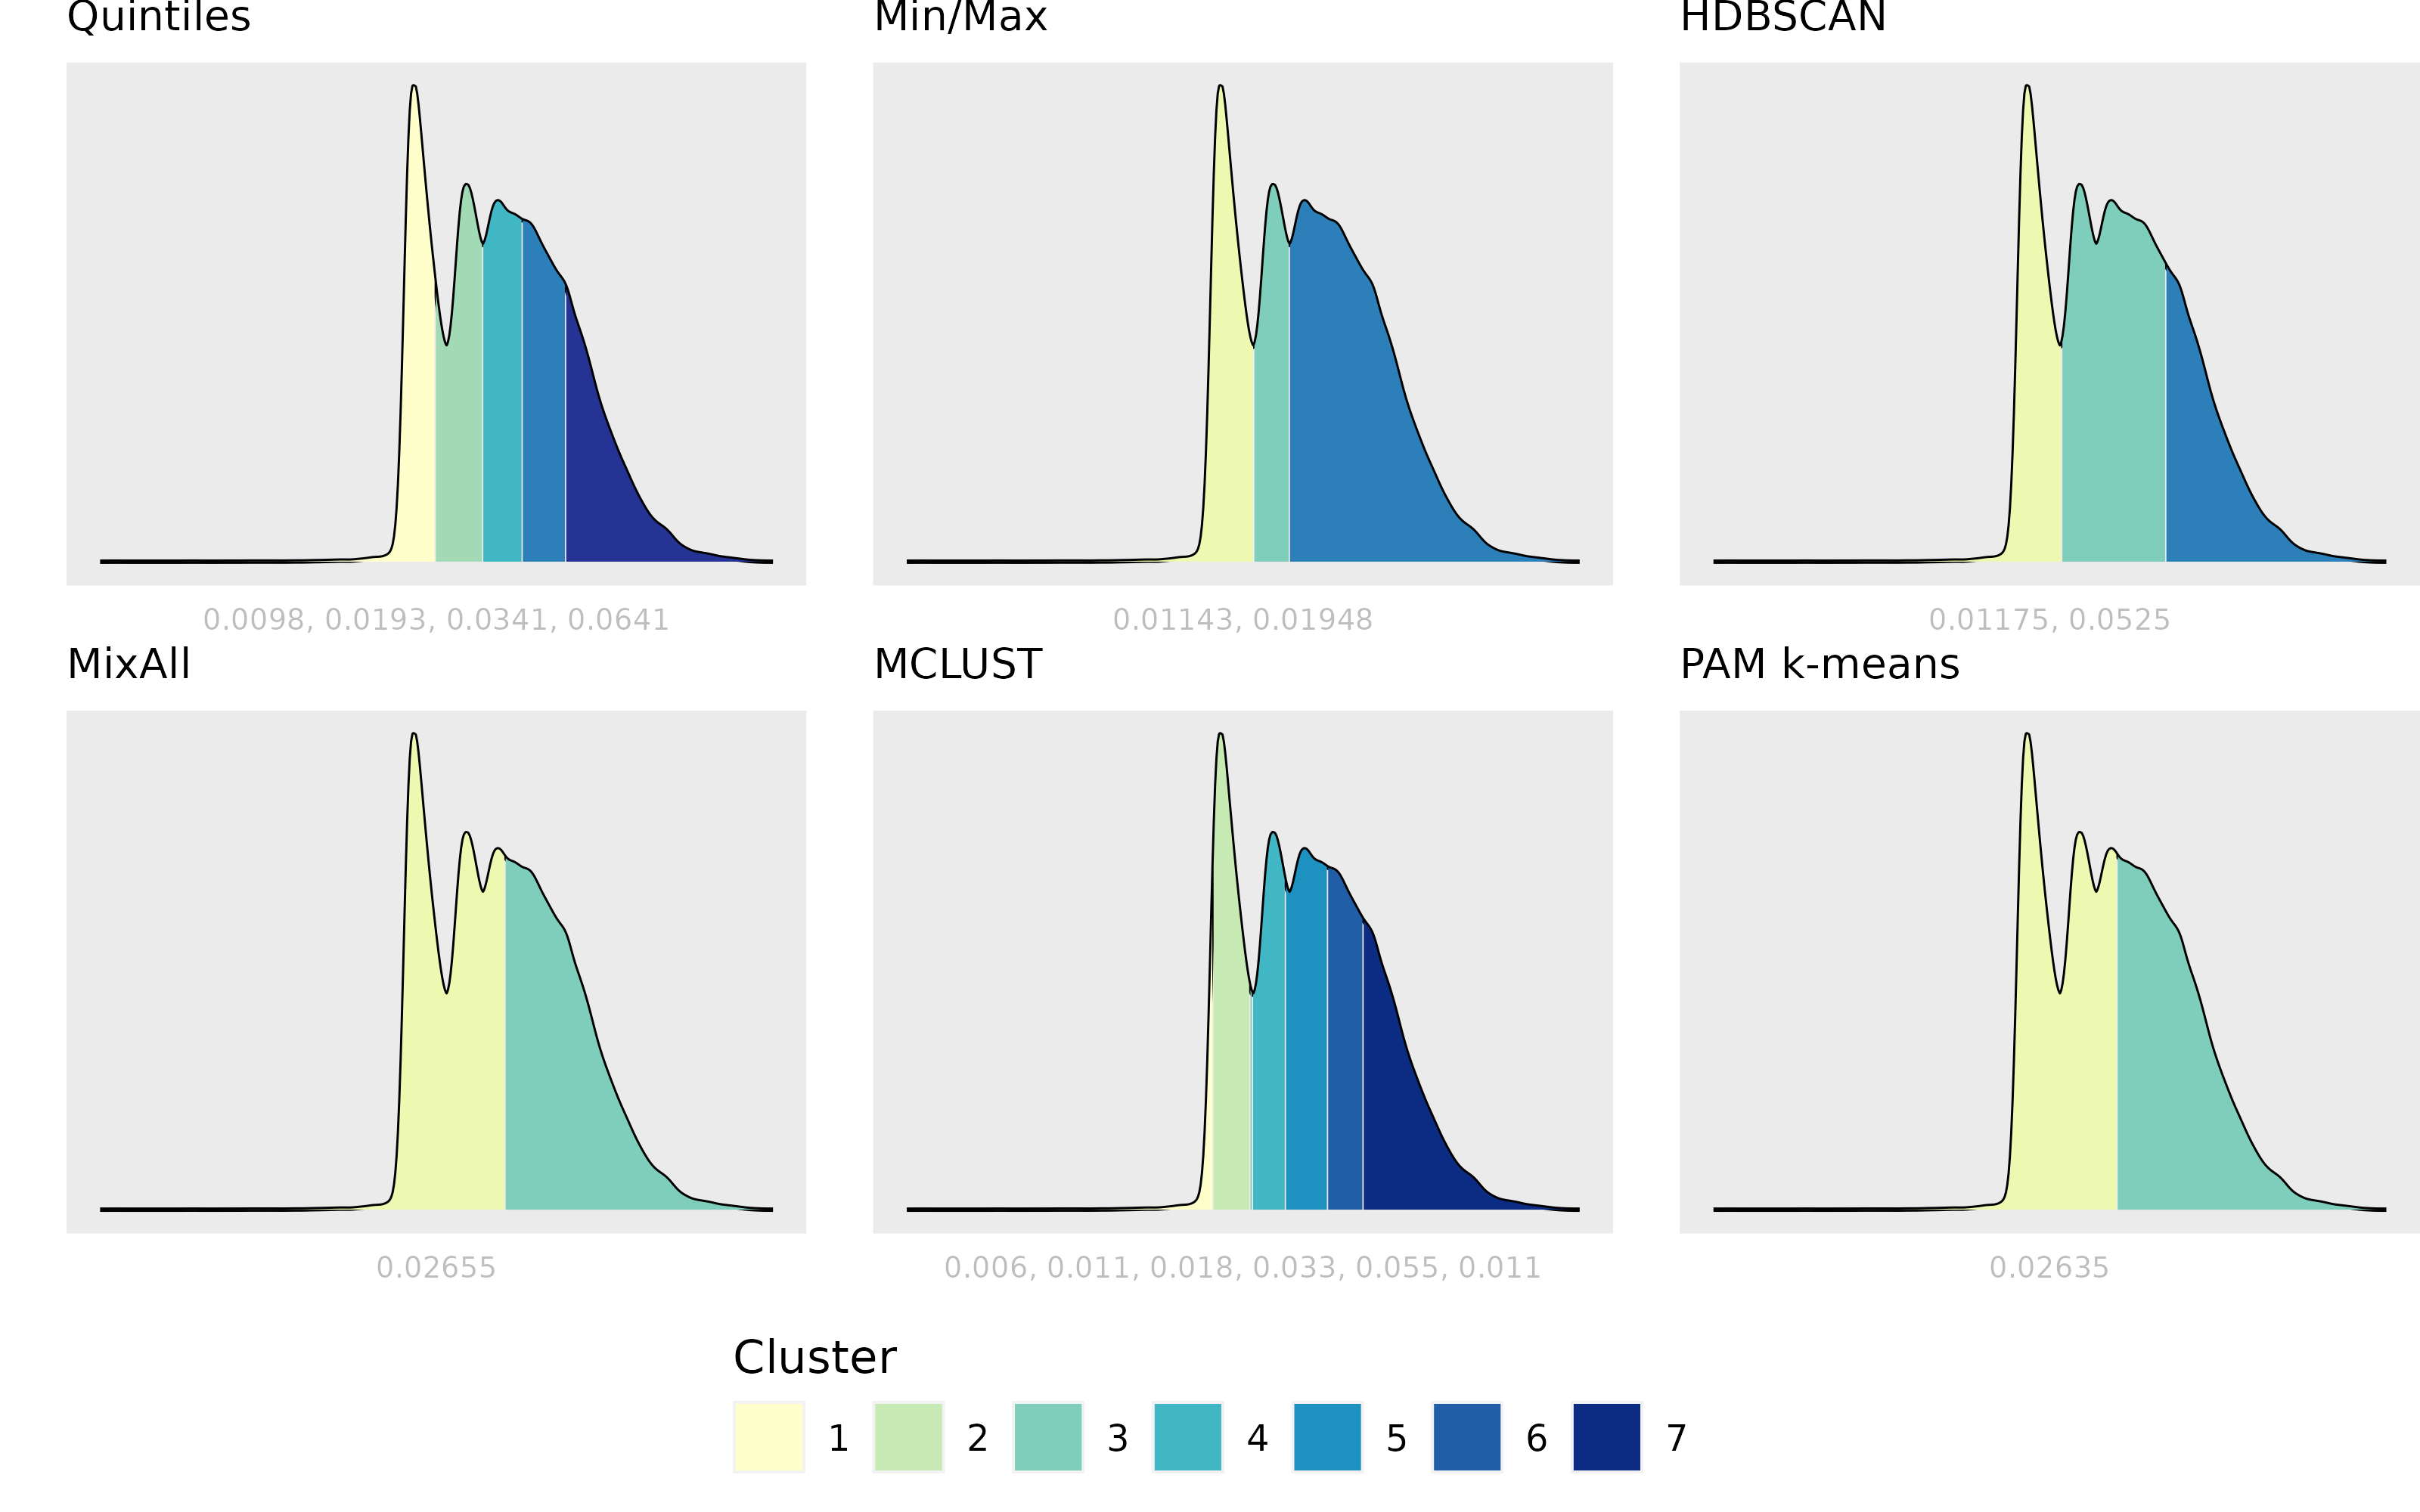
\includegraphics[width=\textwidth]{./cutoffs/by_amenity/Pharmacy_cutoffs.png}
\caption[Pharmacy cutoffs]{Cut-offs values shown on the log-transformed density plots for all clustering approaches pharmacy amenity.}\label{pharmacycutoffs}
\end{figure}










\begin{figure}[H]
\centering
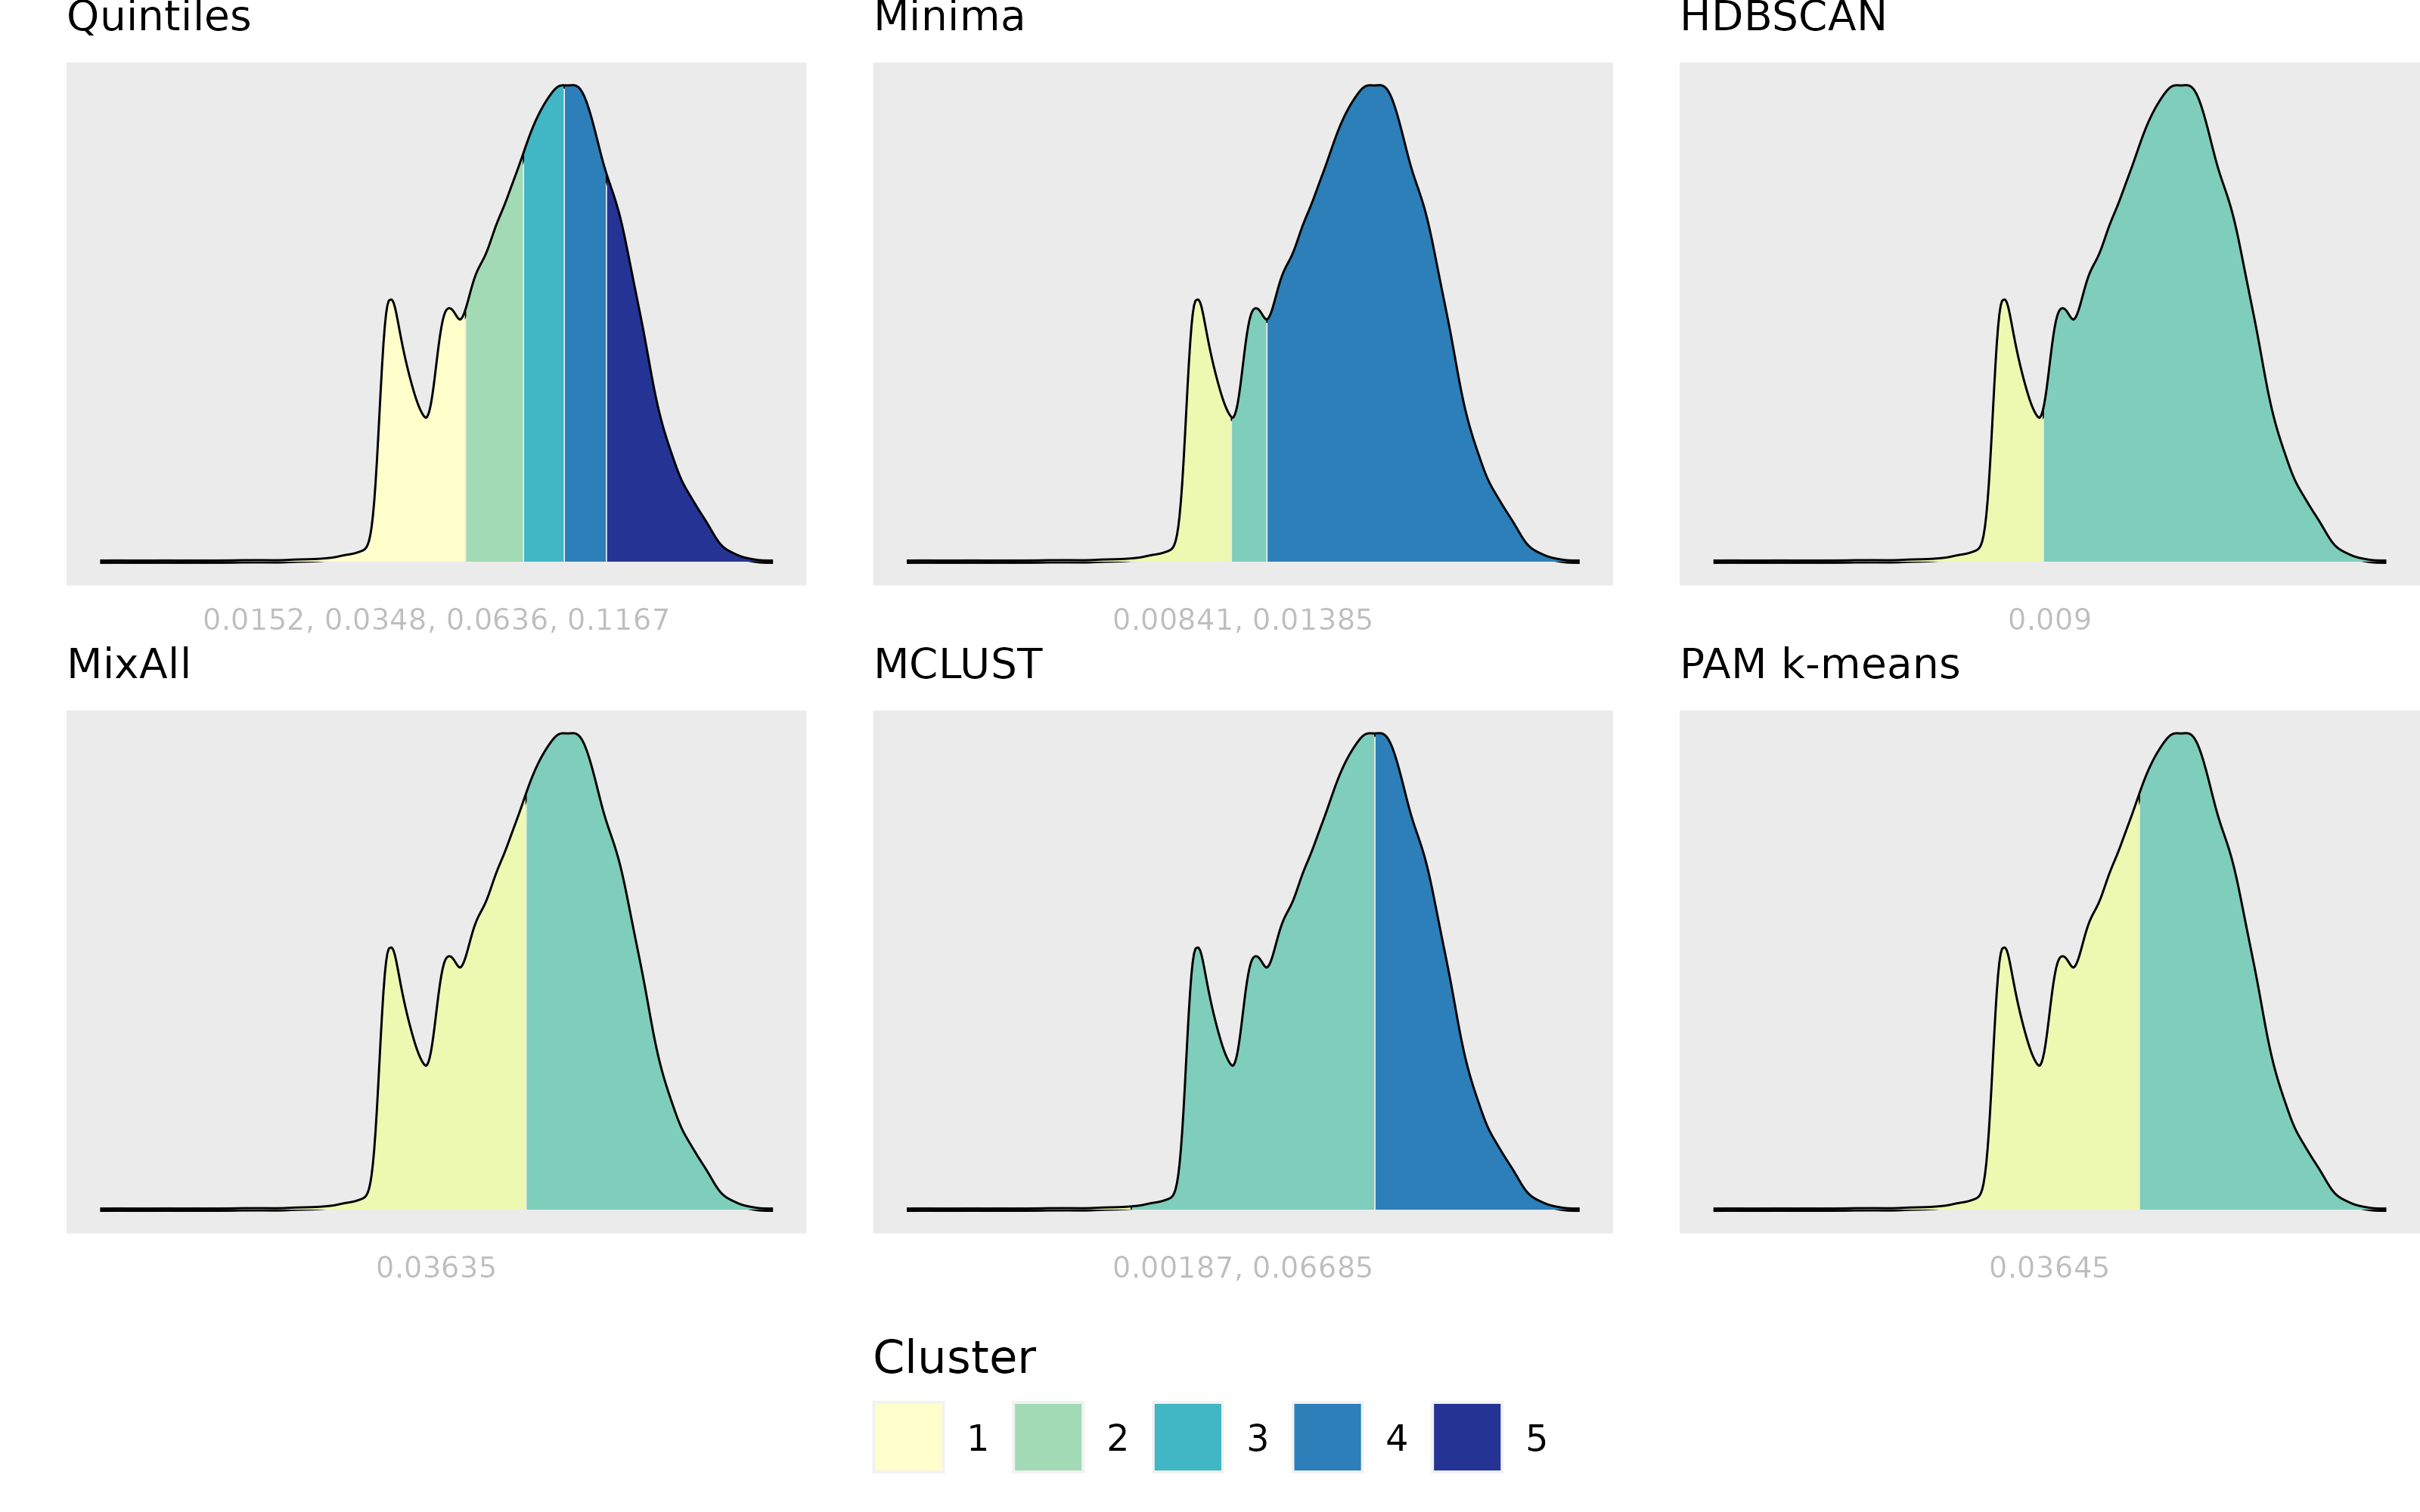
\includegraphics[width=\textwidth]{./cutoffs/by_amenity/Child care_cutoffs.png}
\caption[Child care cutoffs]{Cut-offs values shown on the log-transformed density plots for all clustering approaches child care amenity.}\label{childcarecutoffs}
\end{figure}










\begin{figure}[H]
\centering
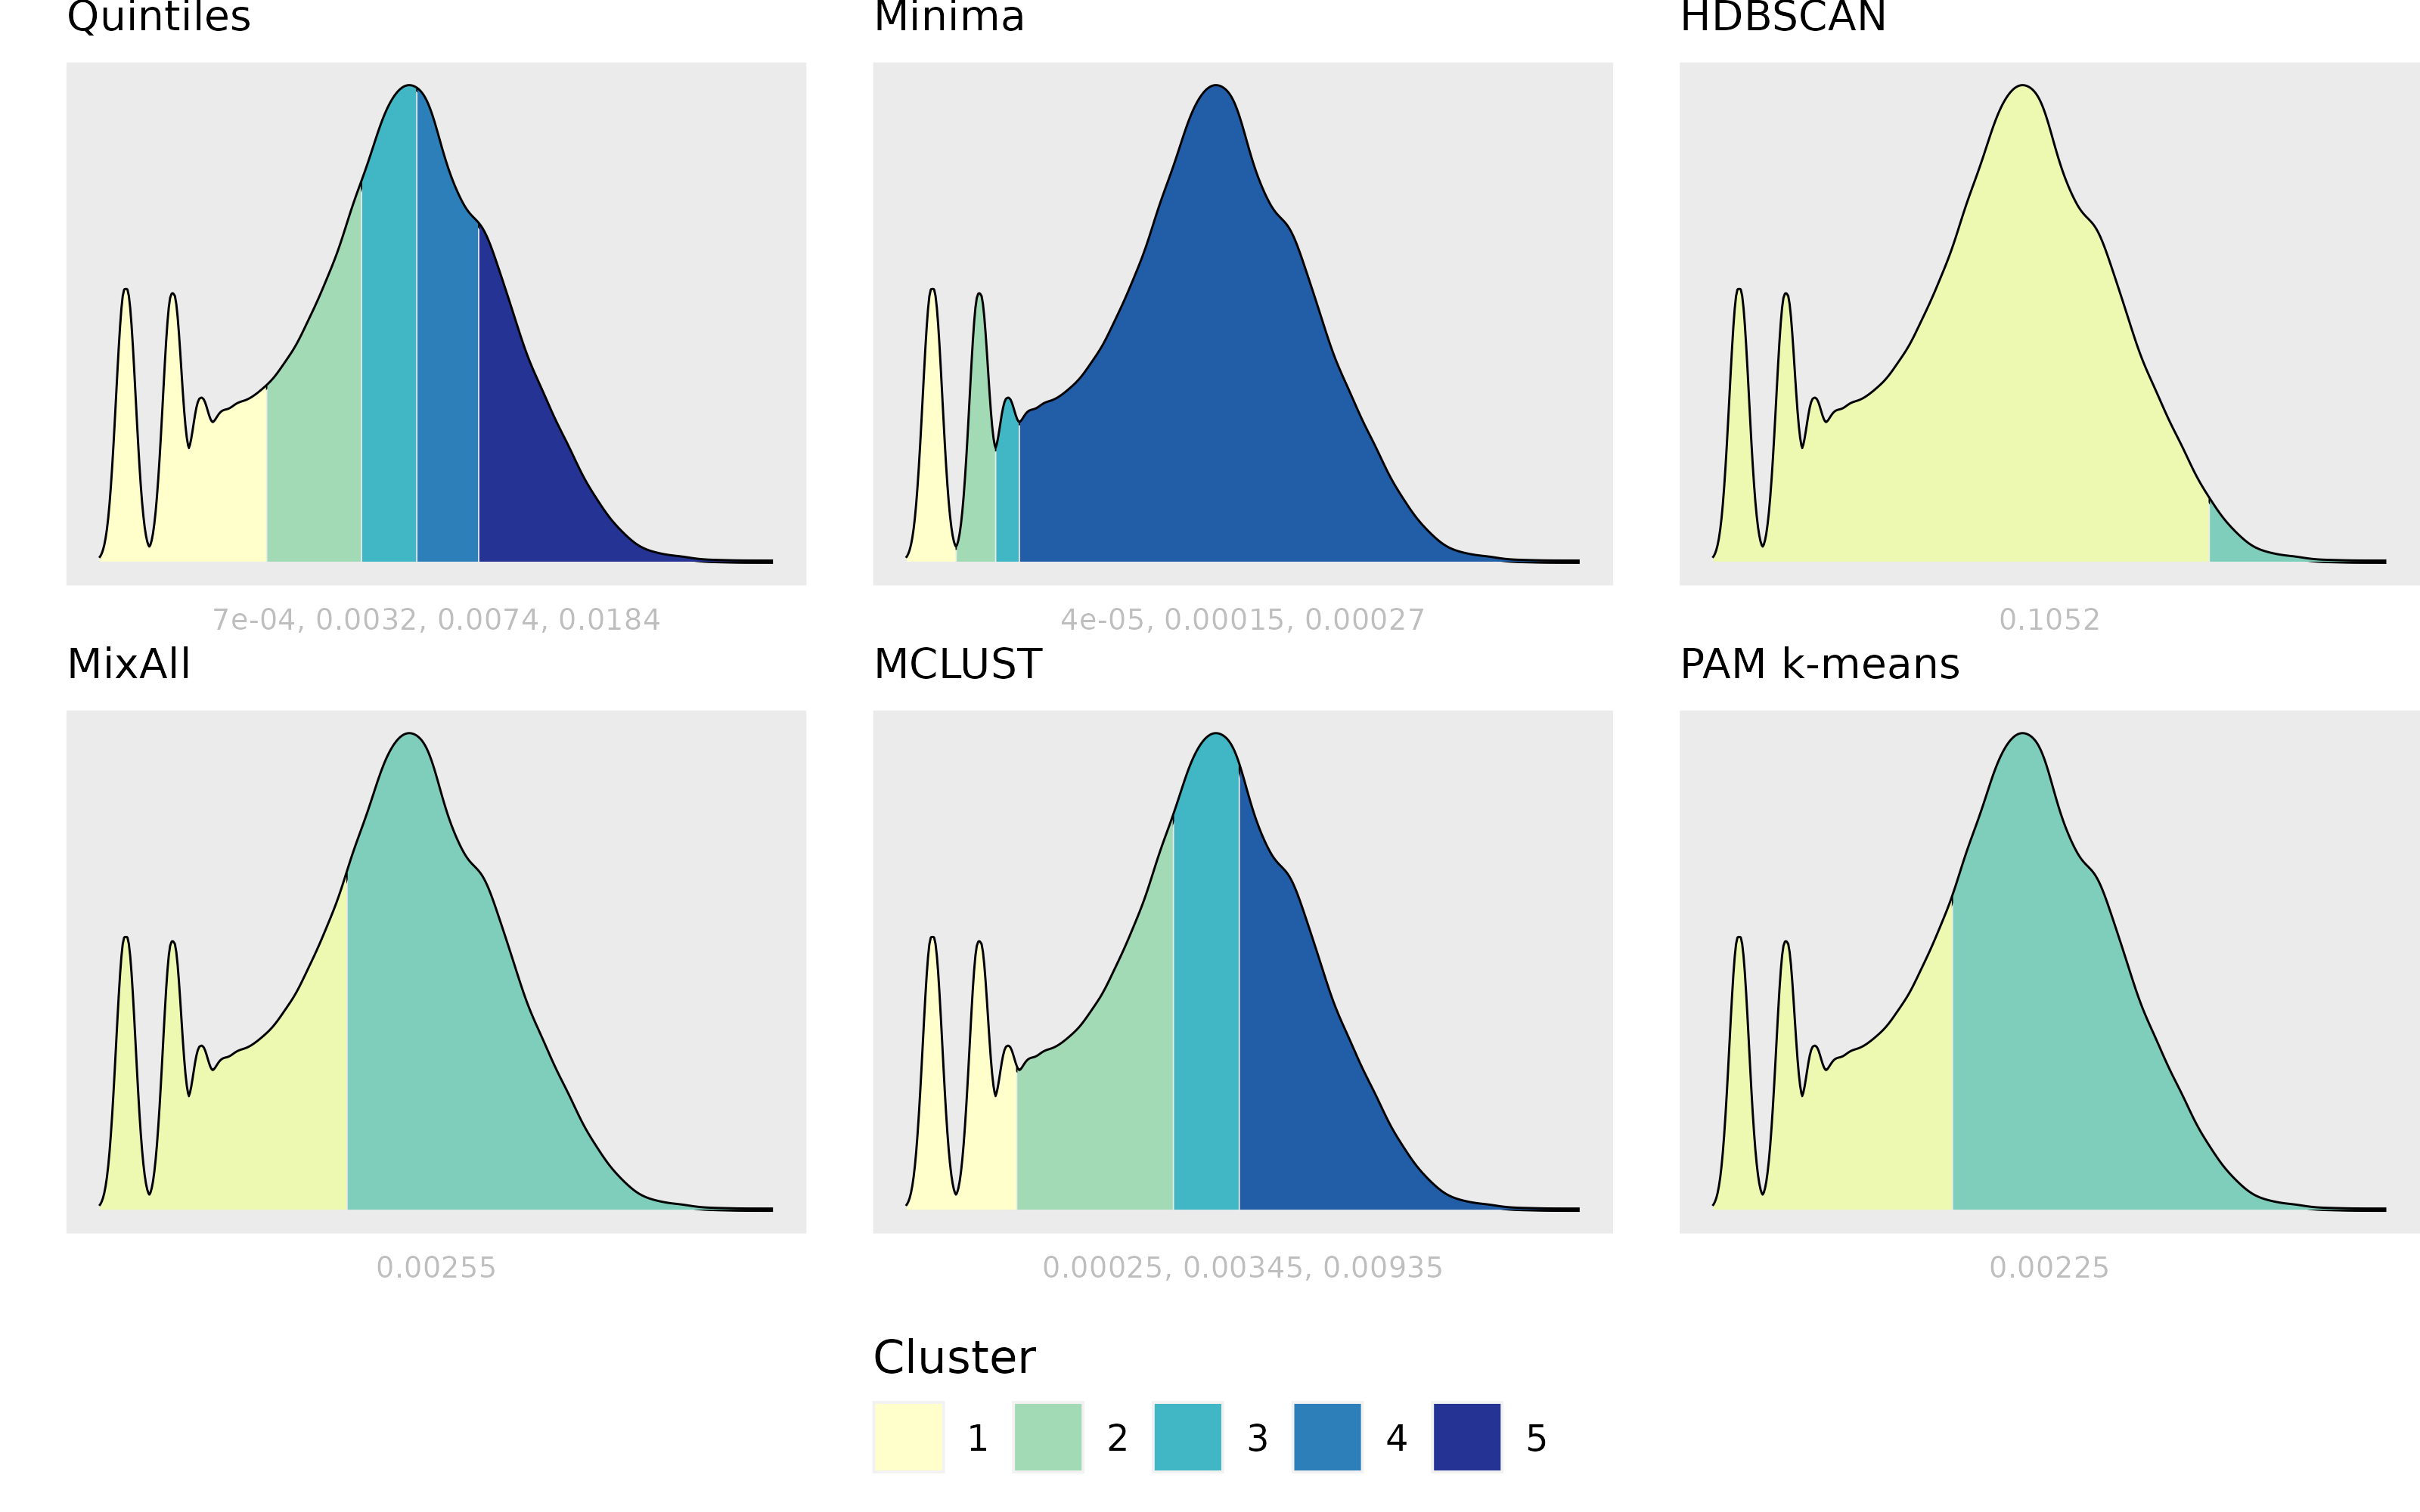
\includegraphics[width=\textwidth]{./cutoffs/by_amenity/Health care_cutoffs.png}
\caption[Health care cutoffs]{Cut-offs values shown on the log-transformed density plots for all clustering approaches health care amenity.}\label{healthcarecutoffs}
\end{figure}










\begin{figure}[H]
\centering
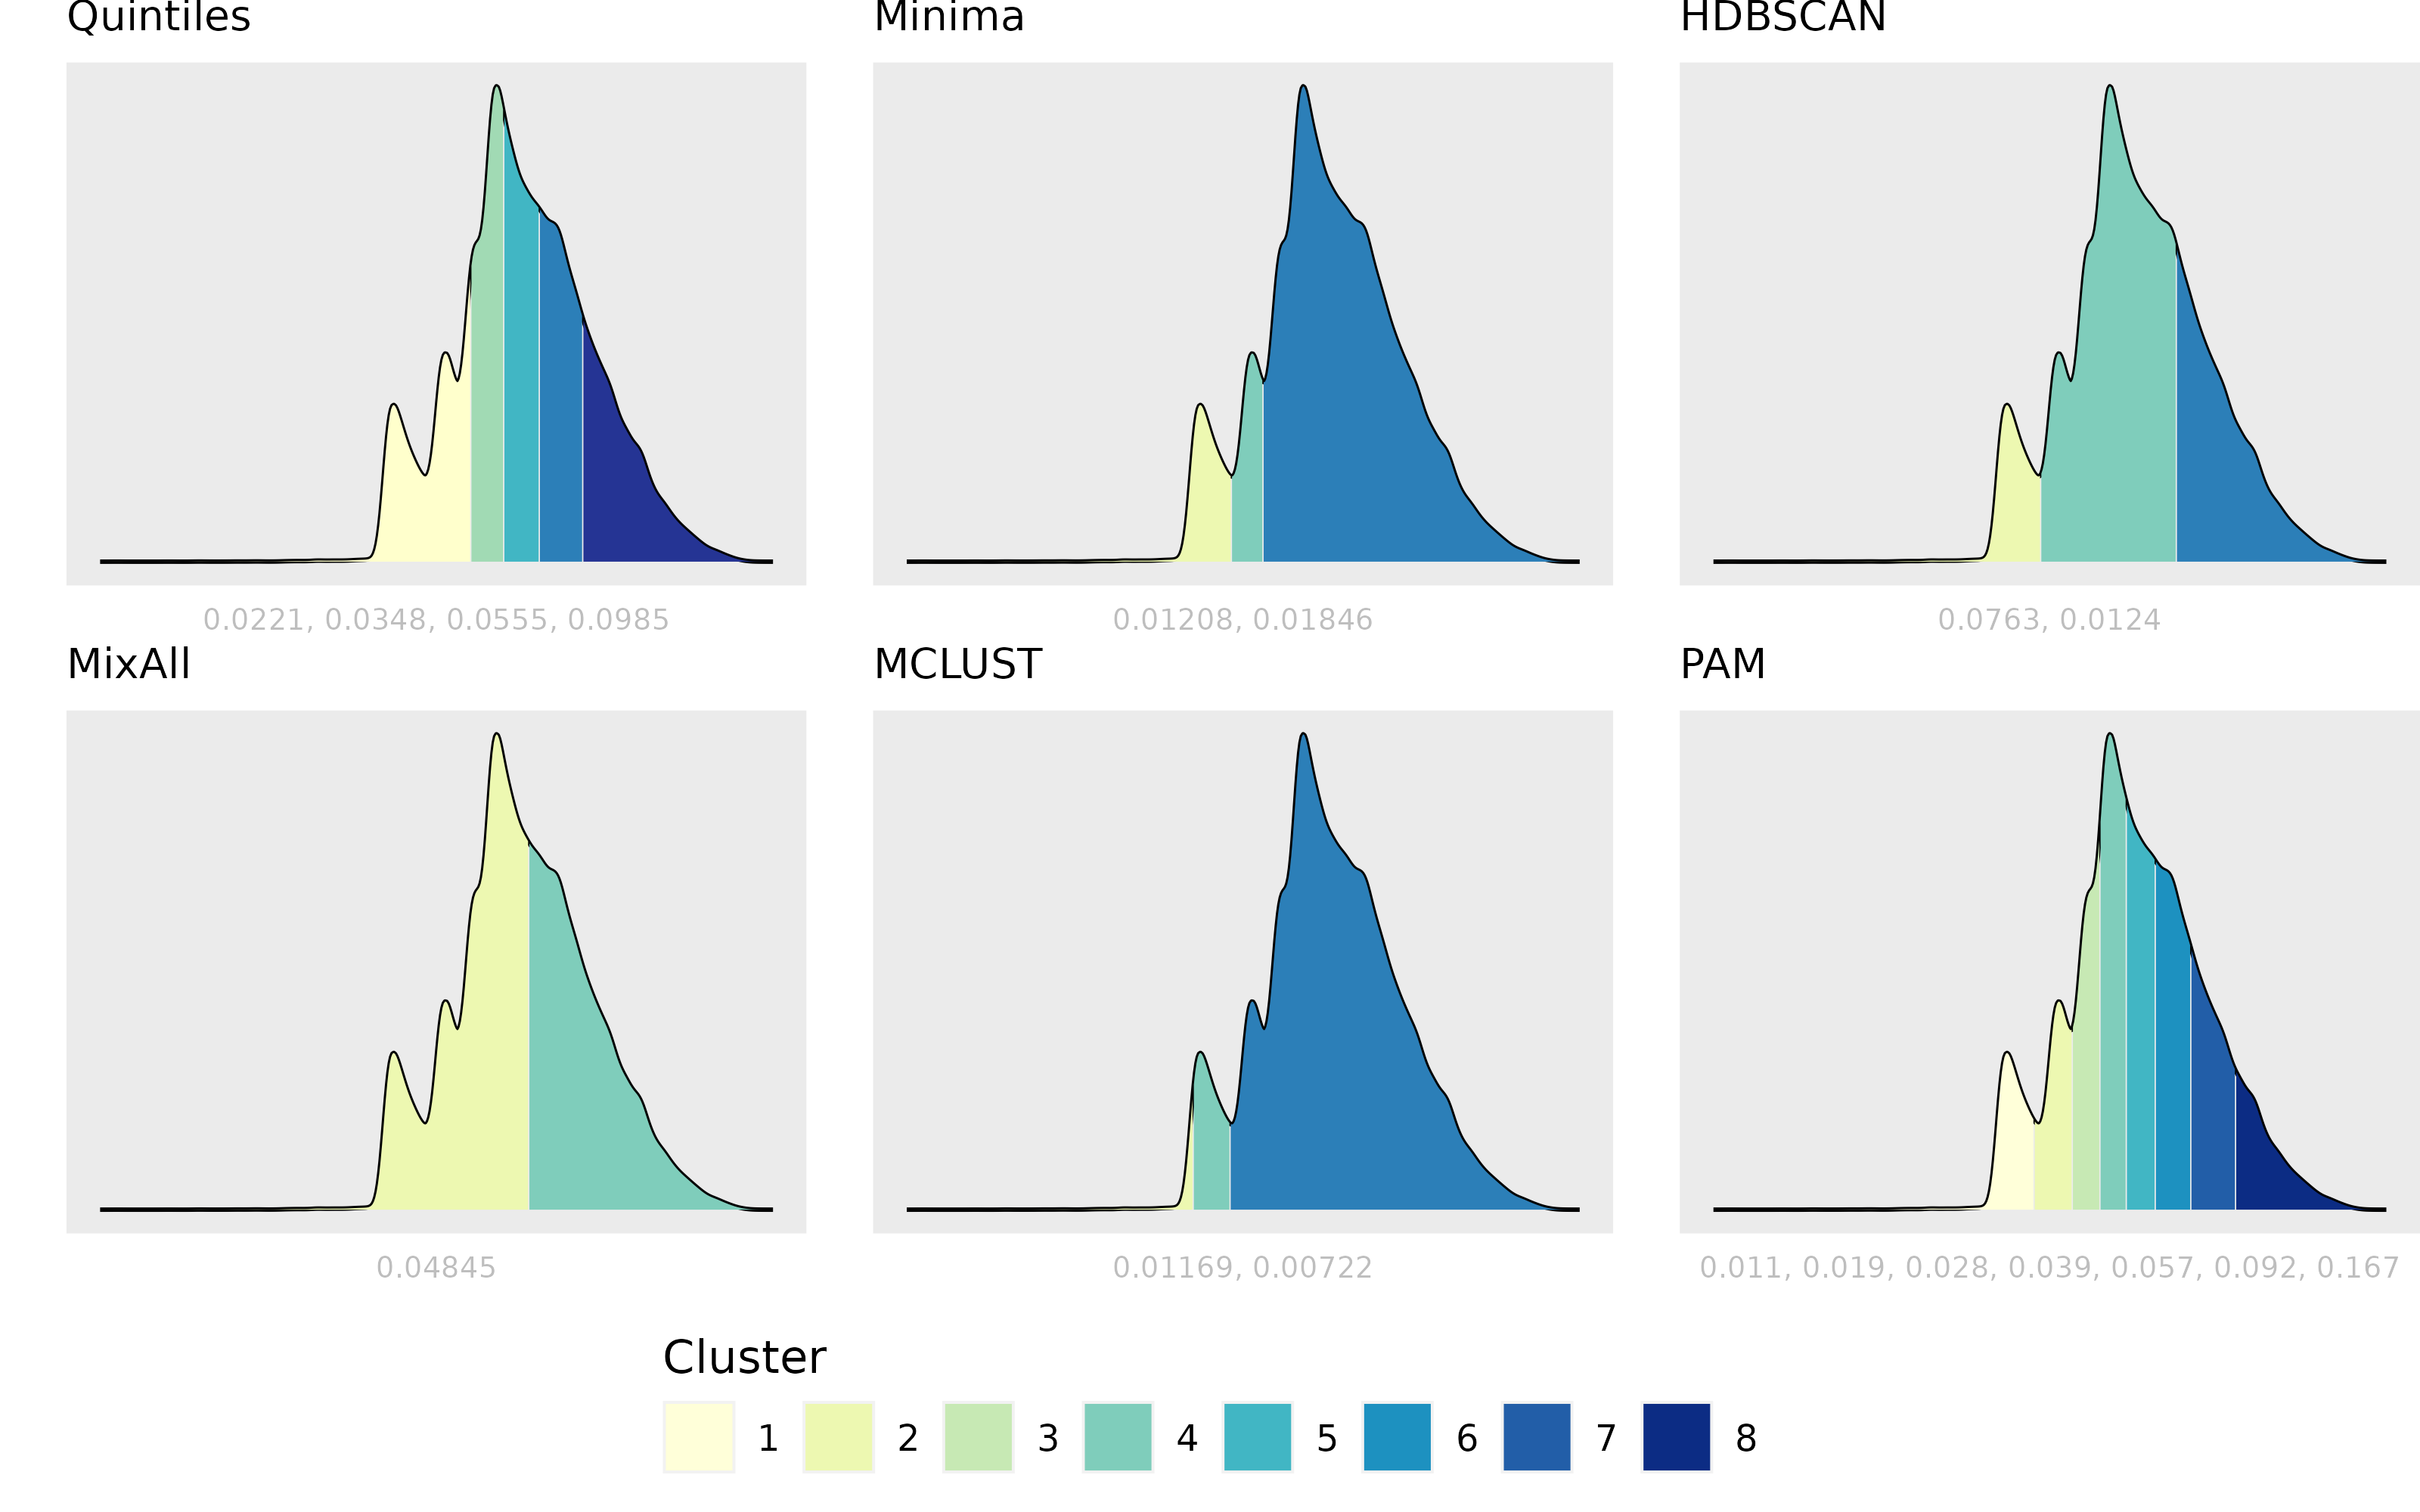
\includegraphics[width=\textwidth]{./cutoffs/by_amenity/Grocery_cutoffs.png}
\caption[Grocery cutoffs]{Cut-offs values shown on the log-transformed density plots for all clustering approaches grocery amenity.}\label{grocerycutoffs}
\end{figure}










\begin{figure}[H]
\centering
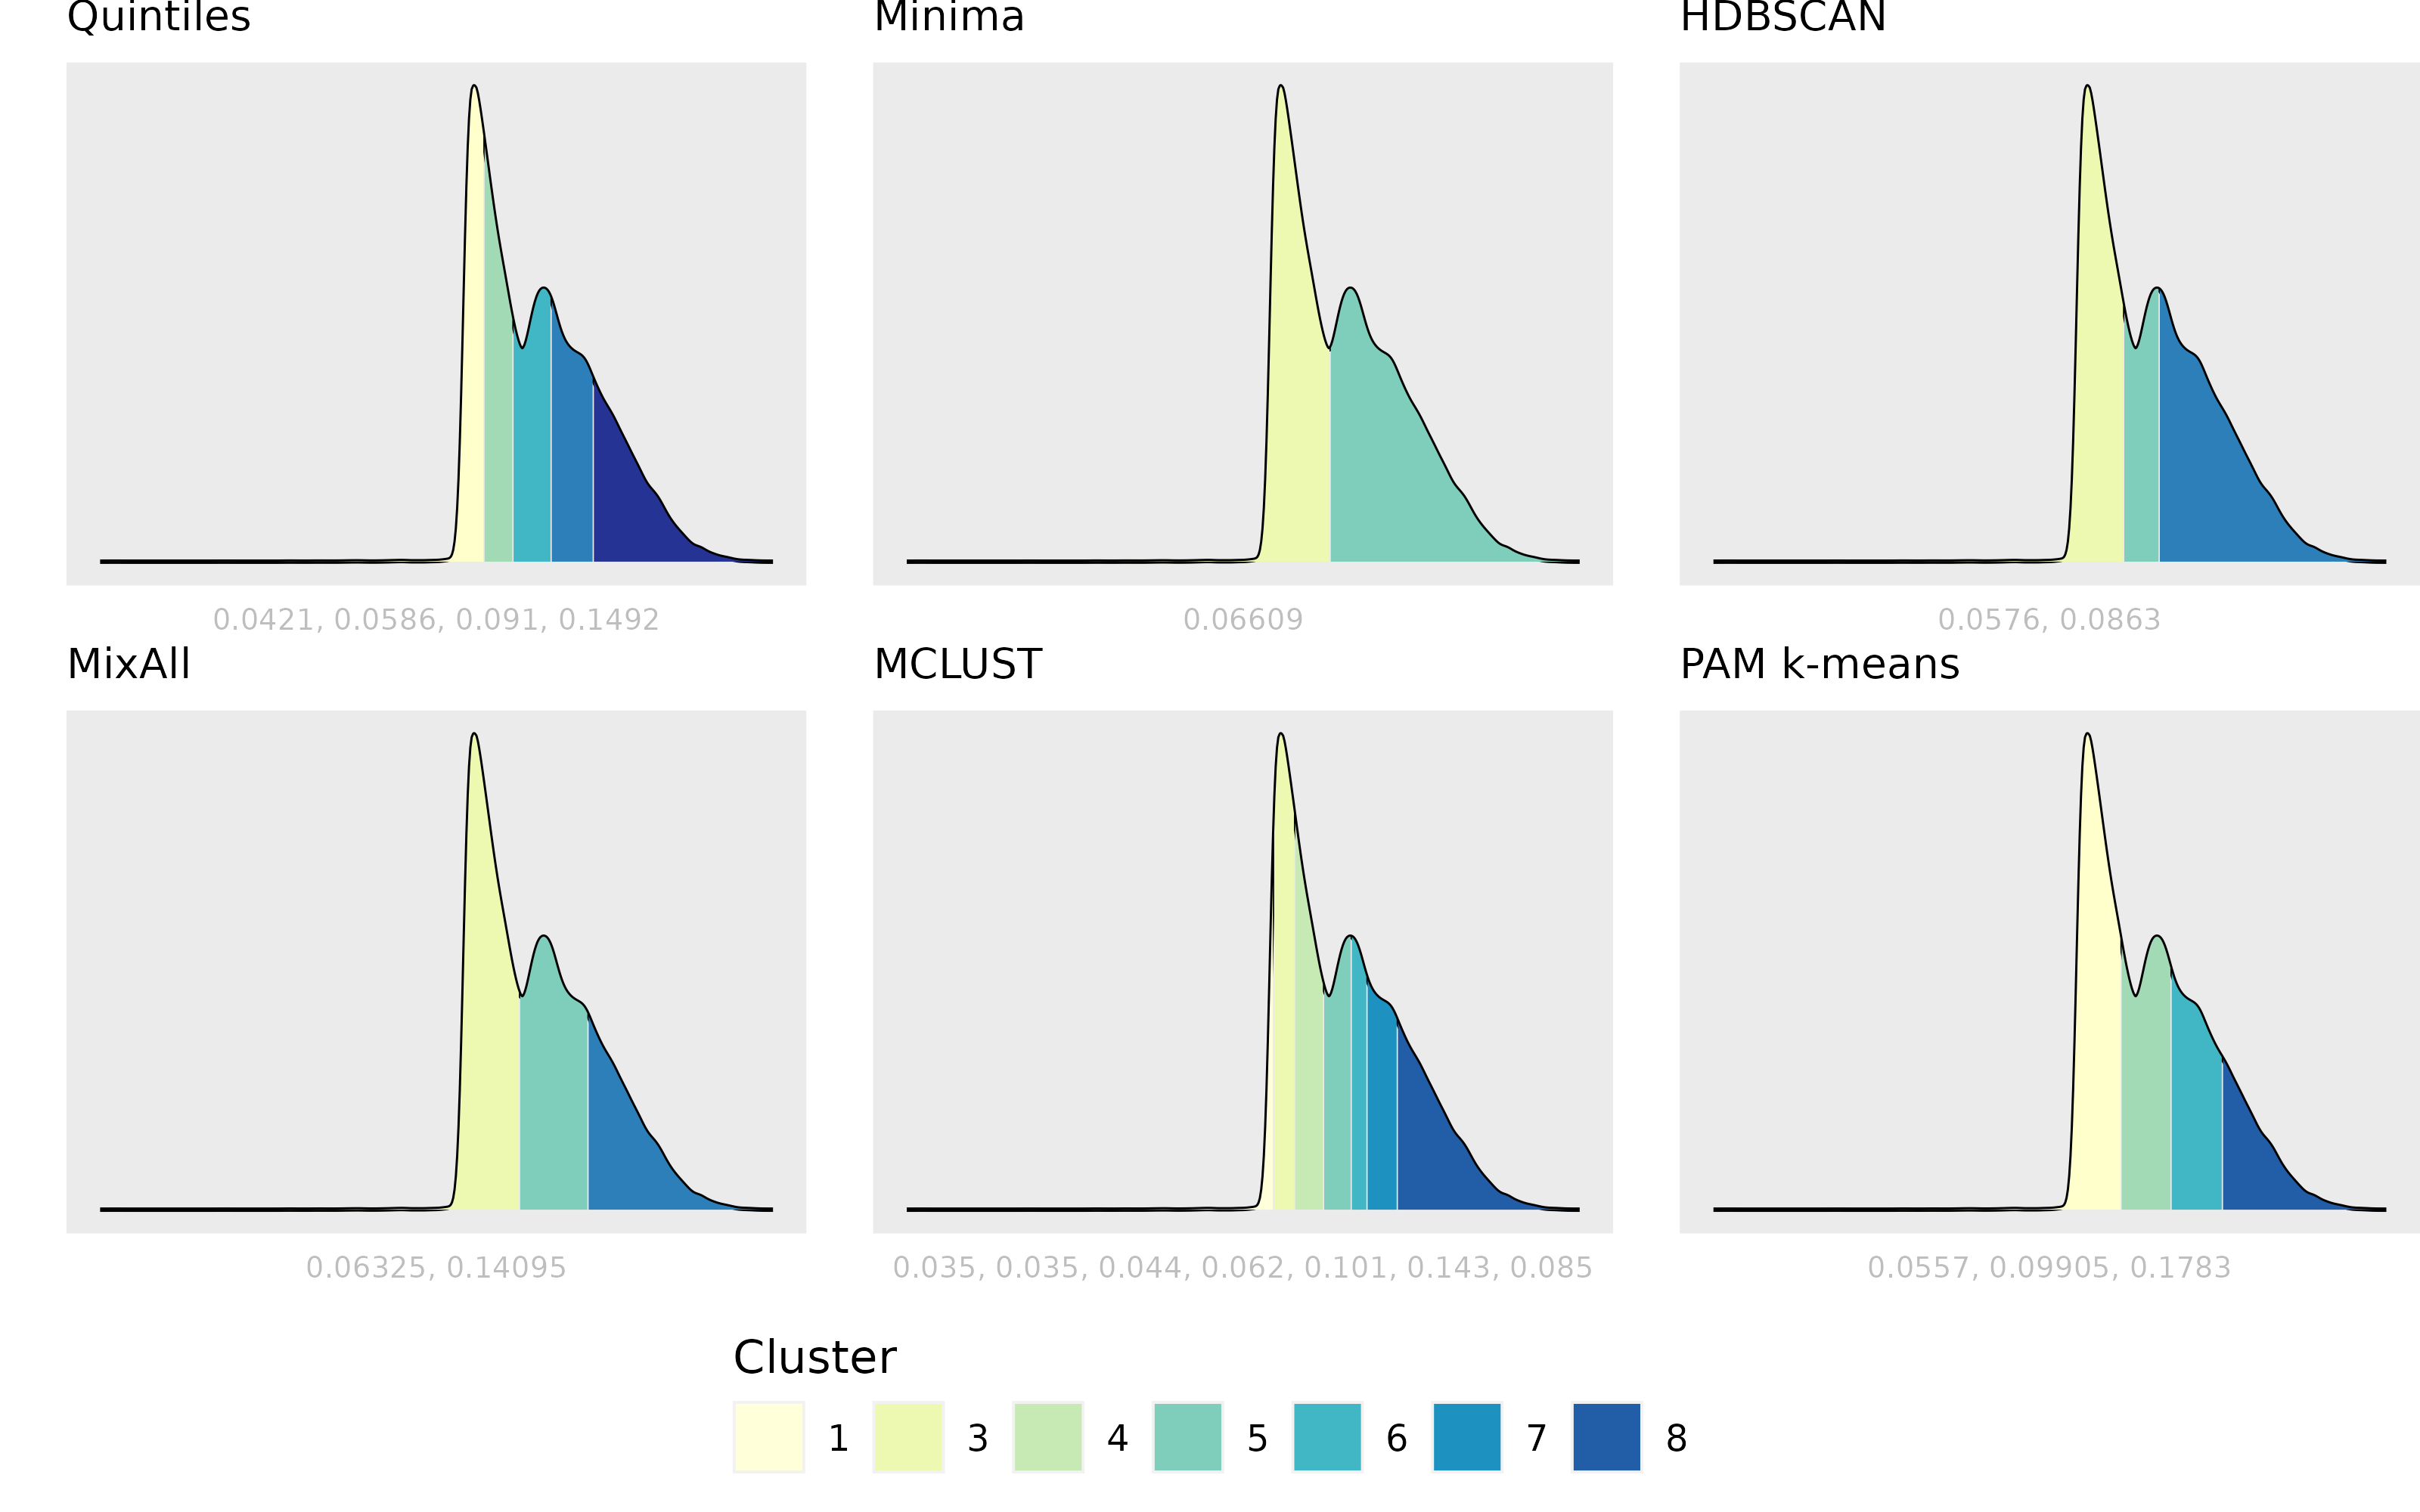
\includegraphics[width=\textwidth]{./cutoffs/by_amenity/Secondary Education_cutoffs.png}
\caption[Secondary education cutoffs]{Cut-offs values shown on the log-transformed density plots for all clustering approaches secondary education amenity.}\label{seceduccutoffs}
\end{figure}










\begin{figure}[H]
\centering
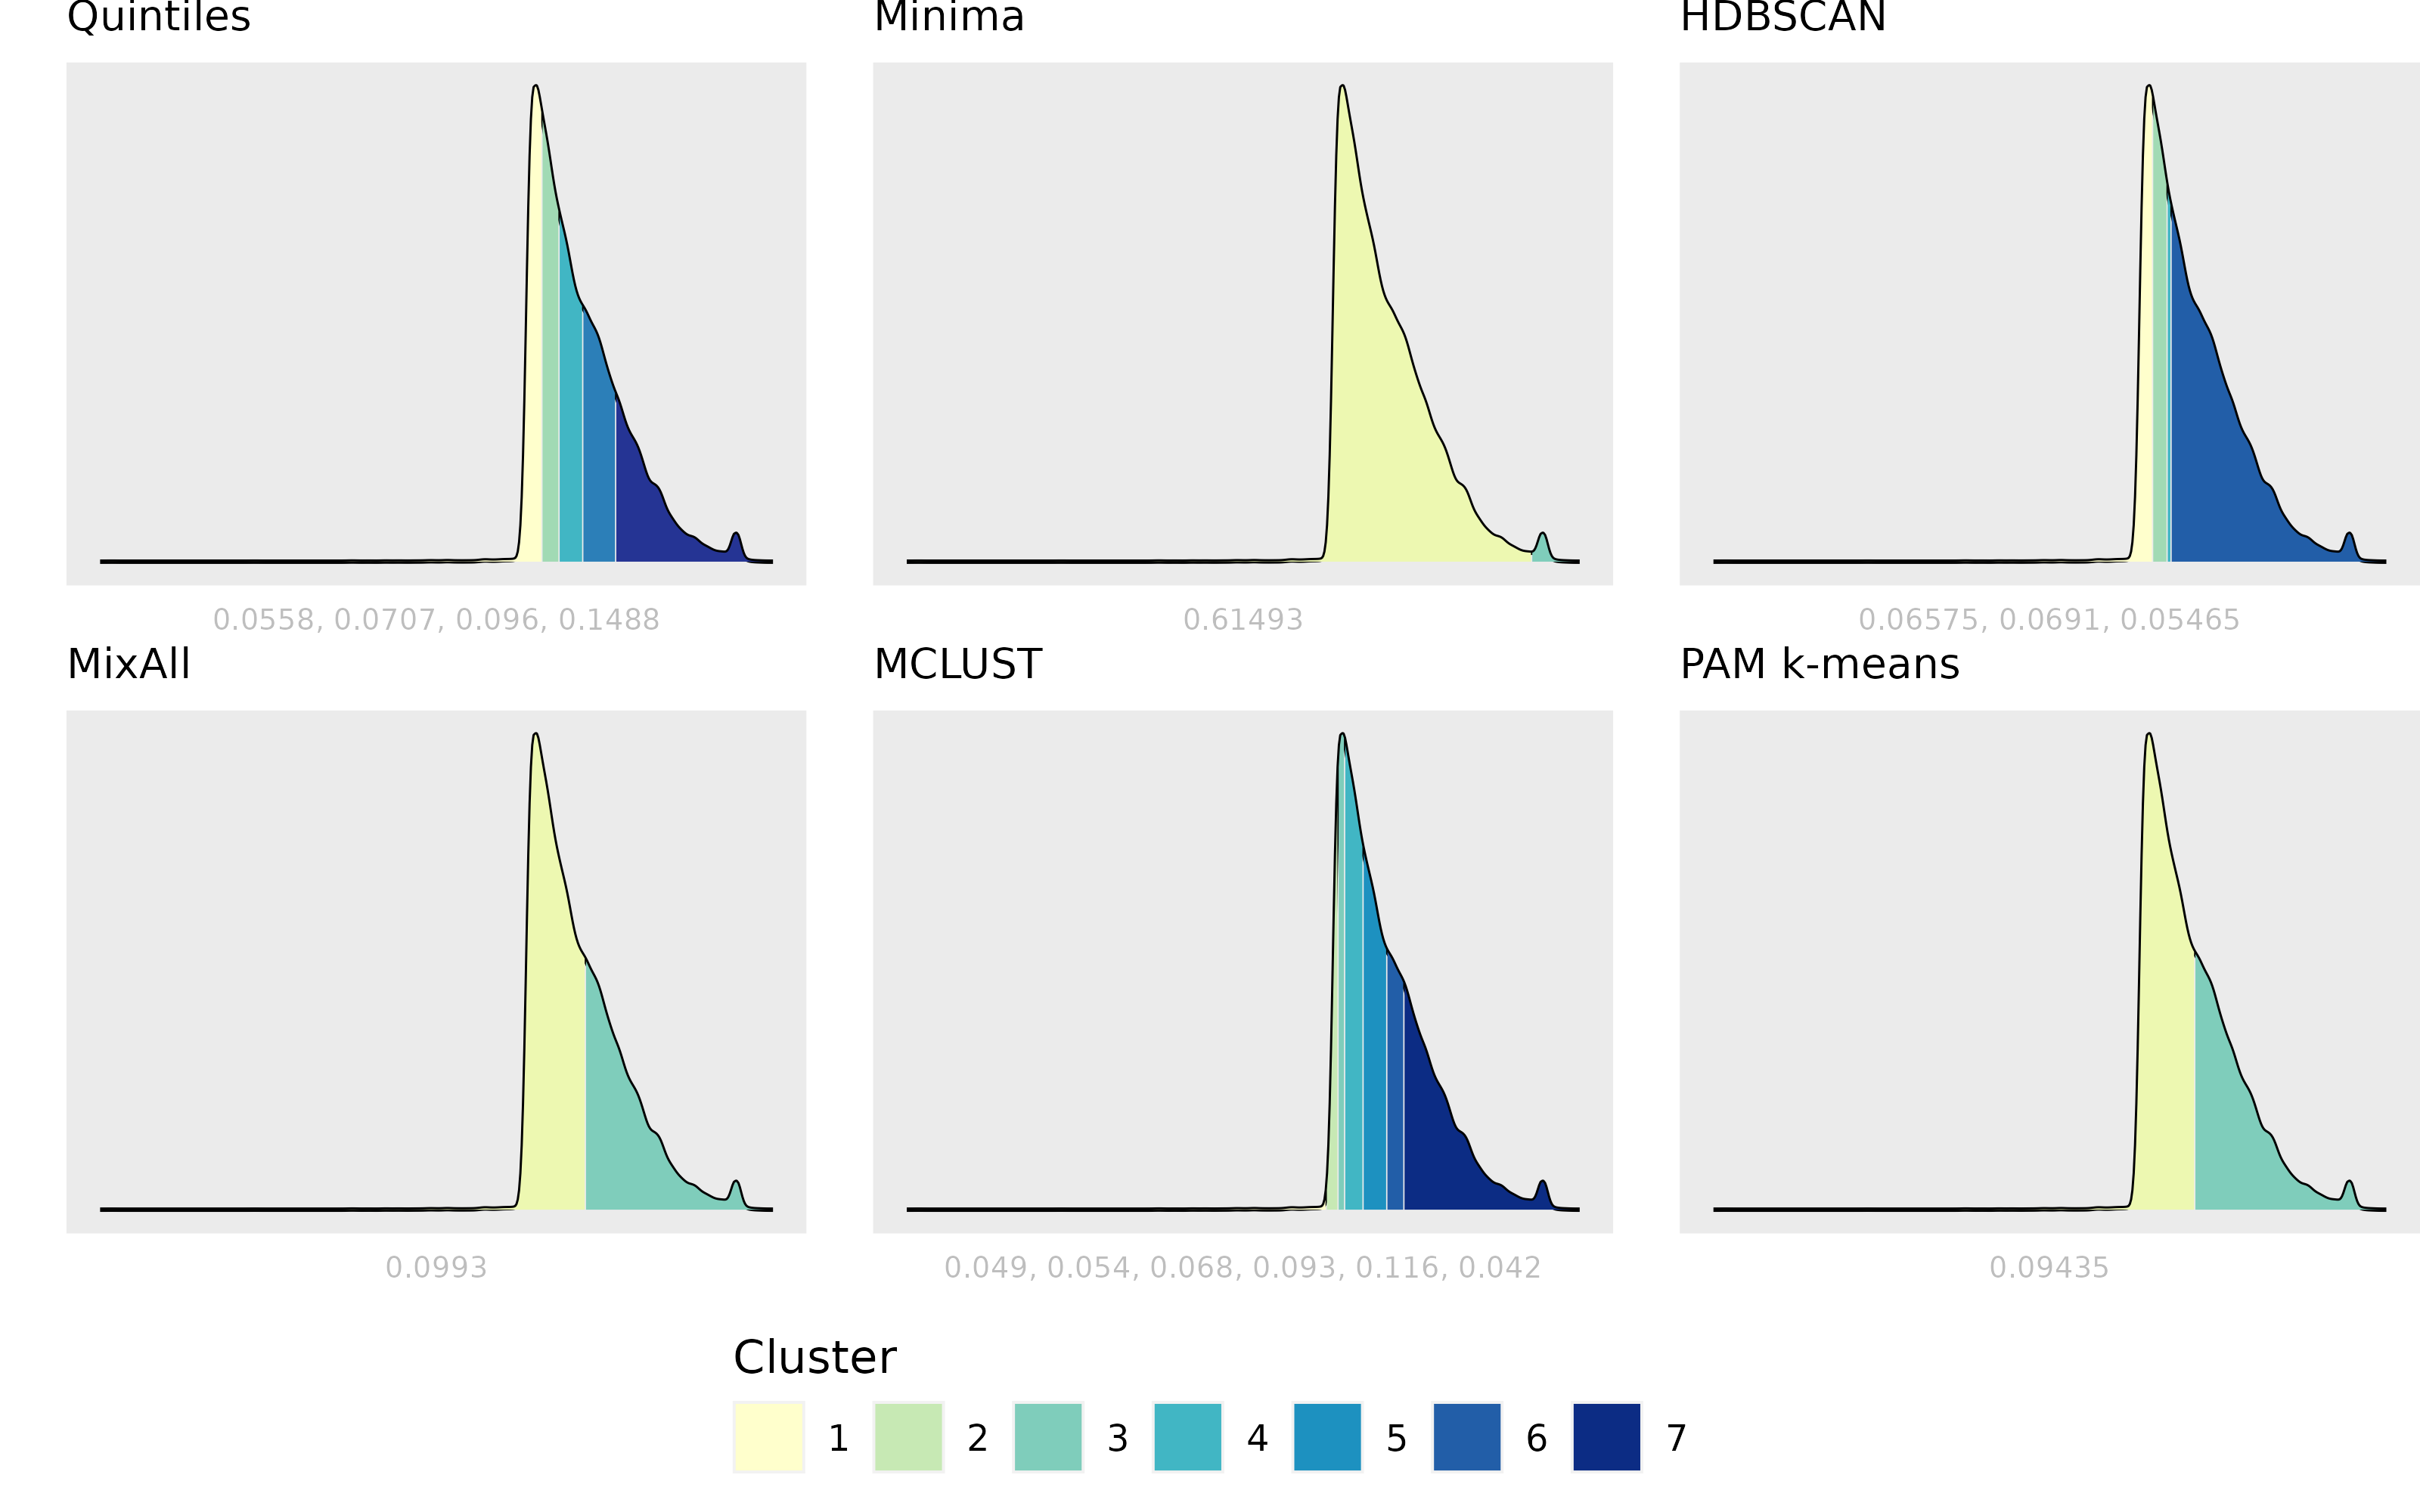
\includegraphics[width=\textwidth]{./cutoffs/by_amenity/Library_cutoffs.png}
\caption[Library cutoffs]{Cut-offs values shown on the log-transformed density plots for all clustering approaches library amenity.}\label{librarycutoffs}
\end{figure}










\begin{figure}[H]
\centering
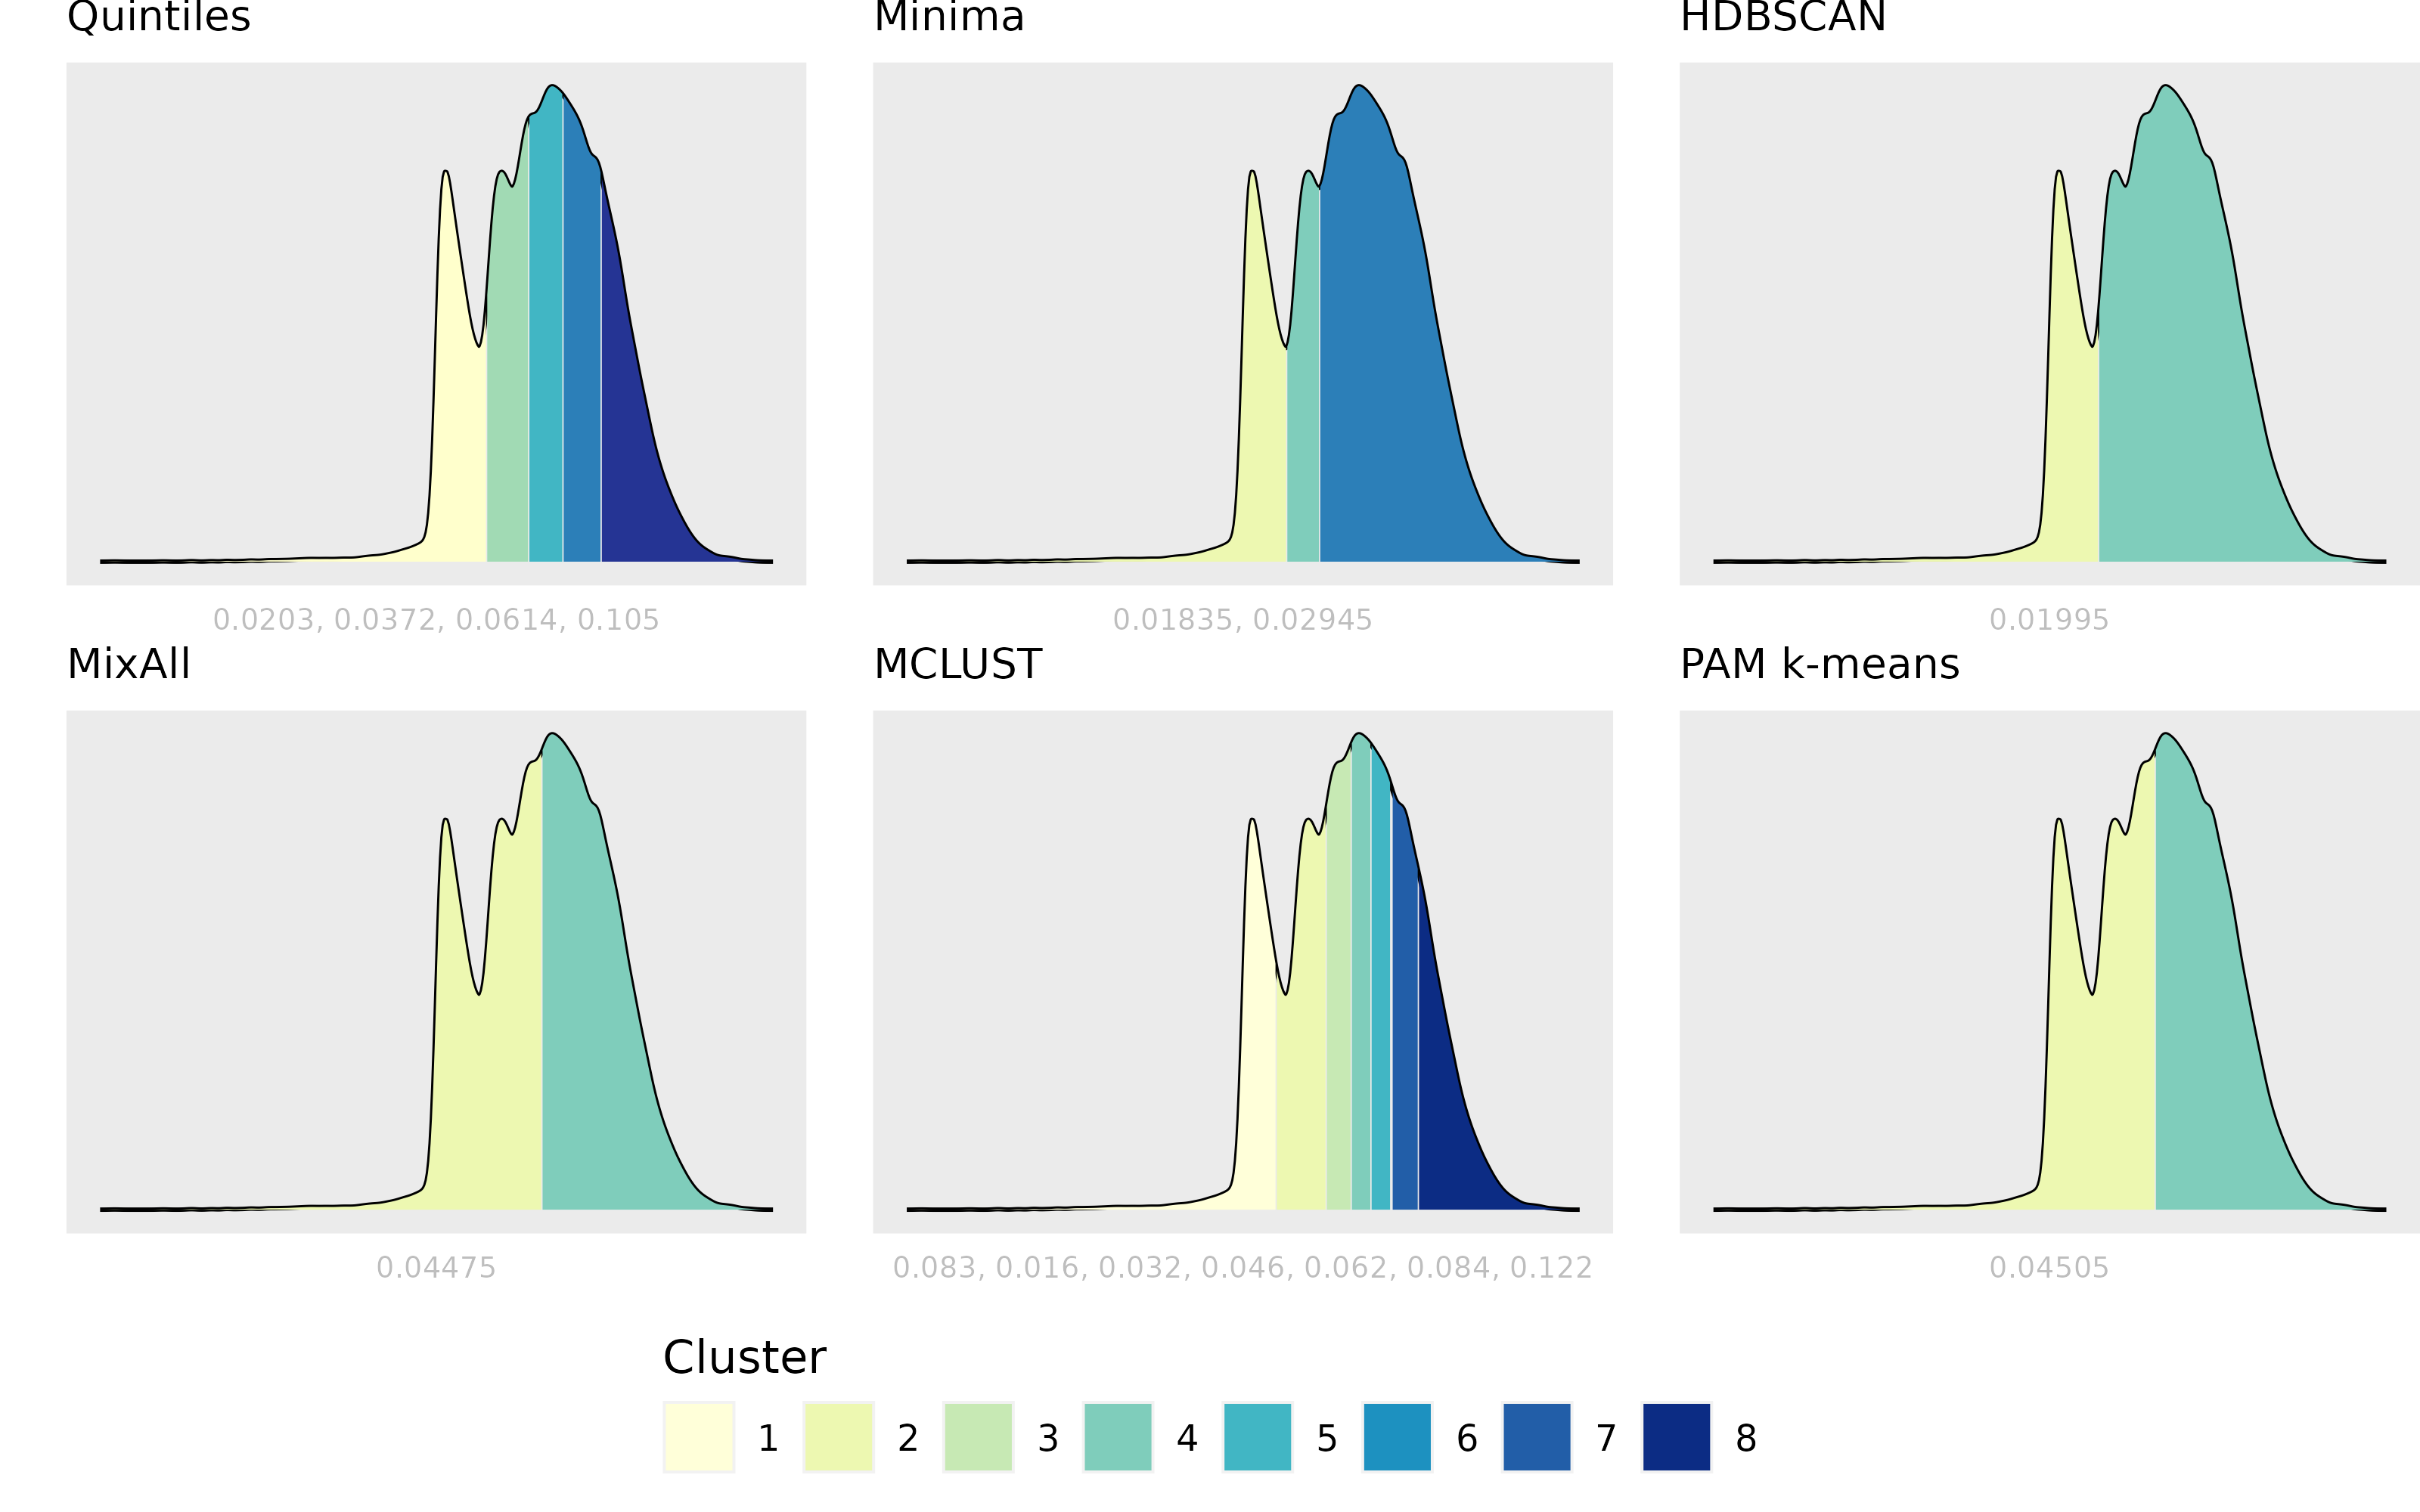
\includegraphics[width=\textwidth]{./cutoffs/by_amenity/Parks_cutoffs.png}
\caption[Parks cutoffs]{Cut-offs values shown on the log-transformed density plots for all clustering approaches parks amenity.}\label{parkscutoffs}
\end{figure}










\begin{figure}[H]
\centering
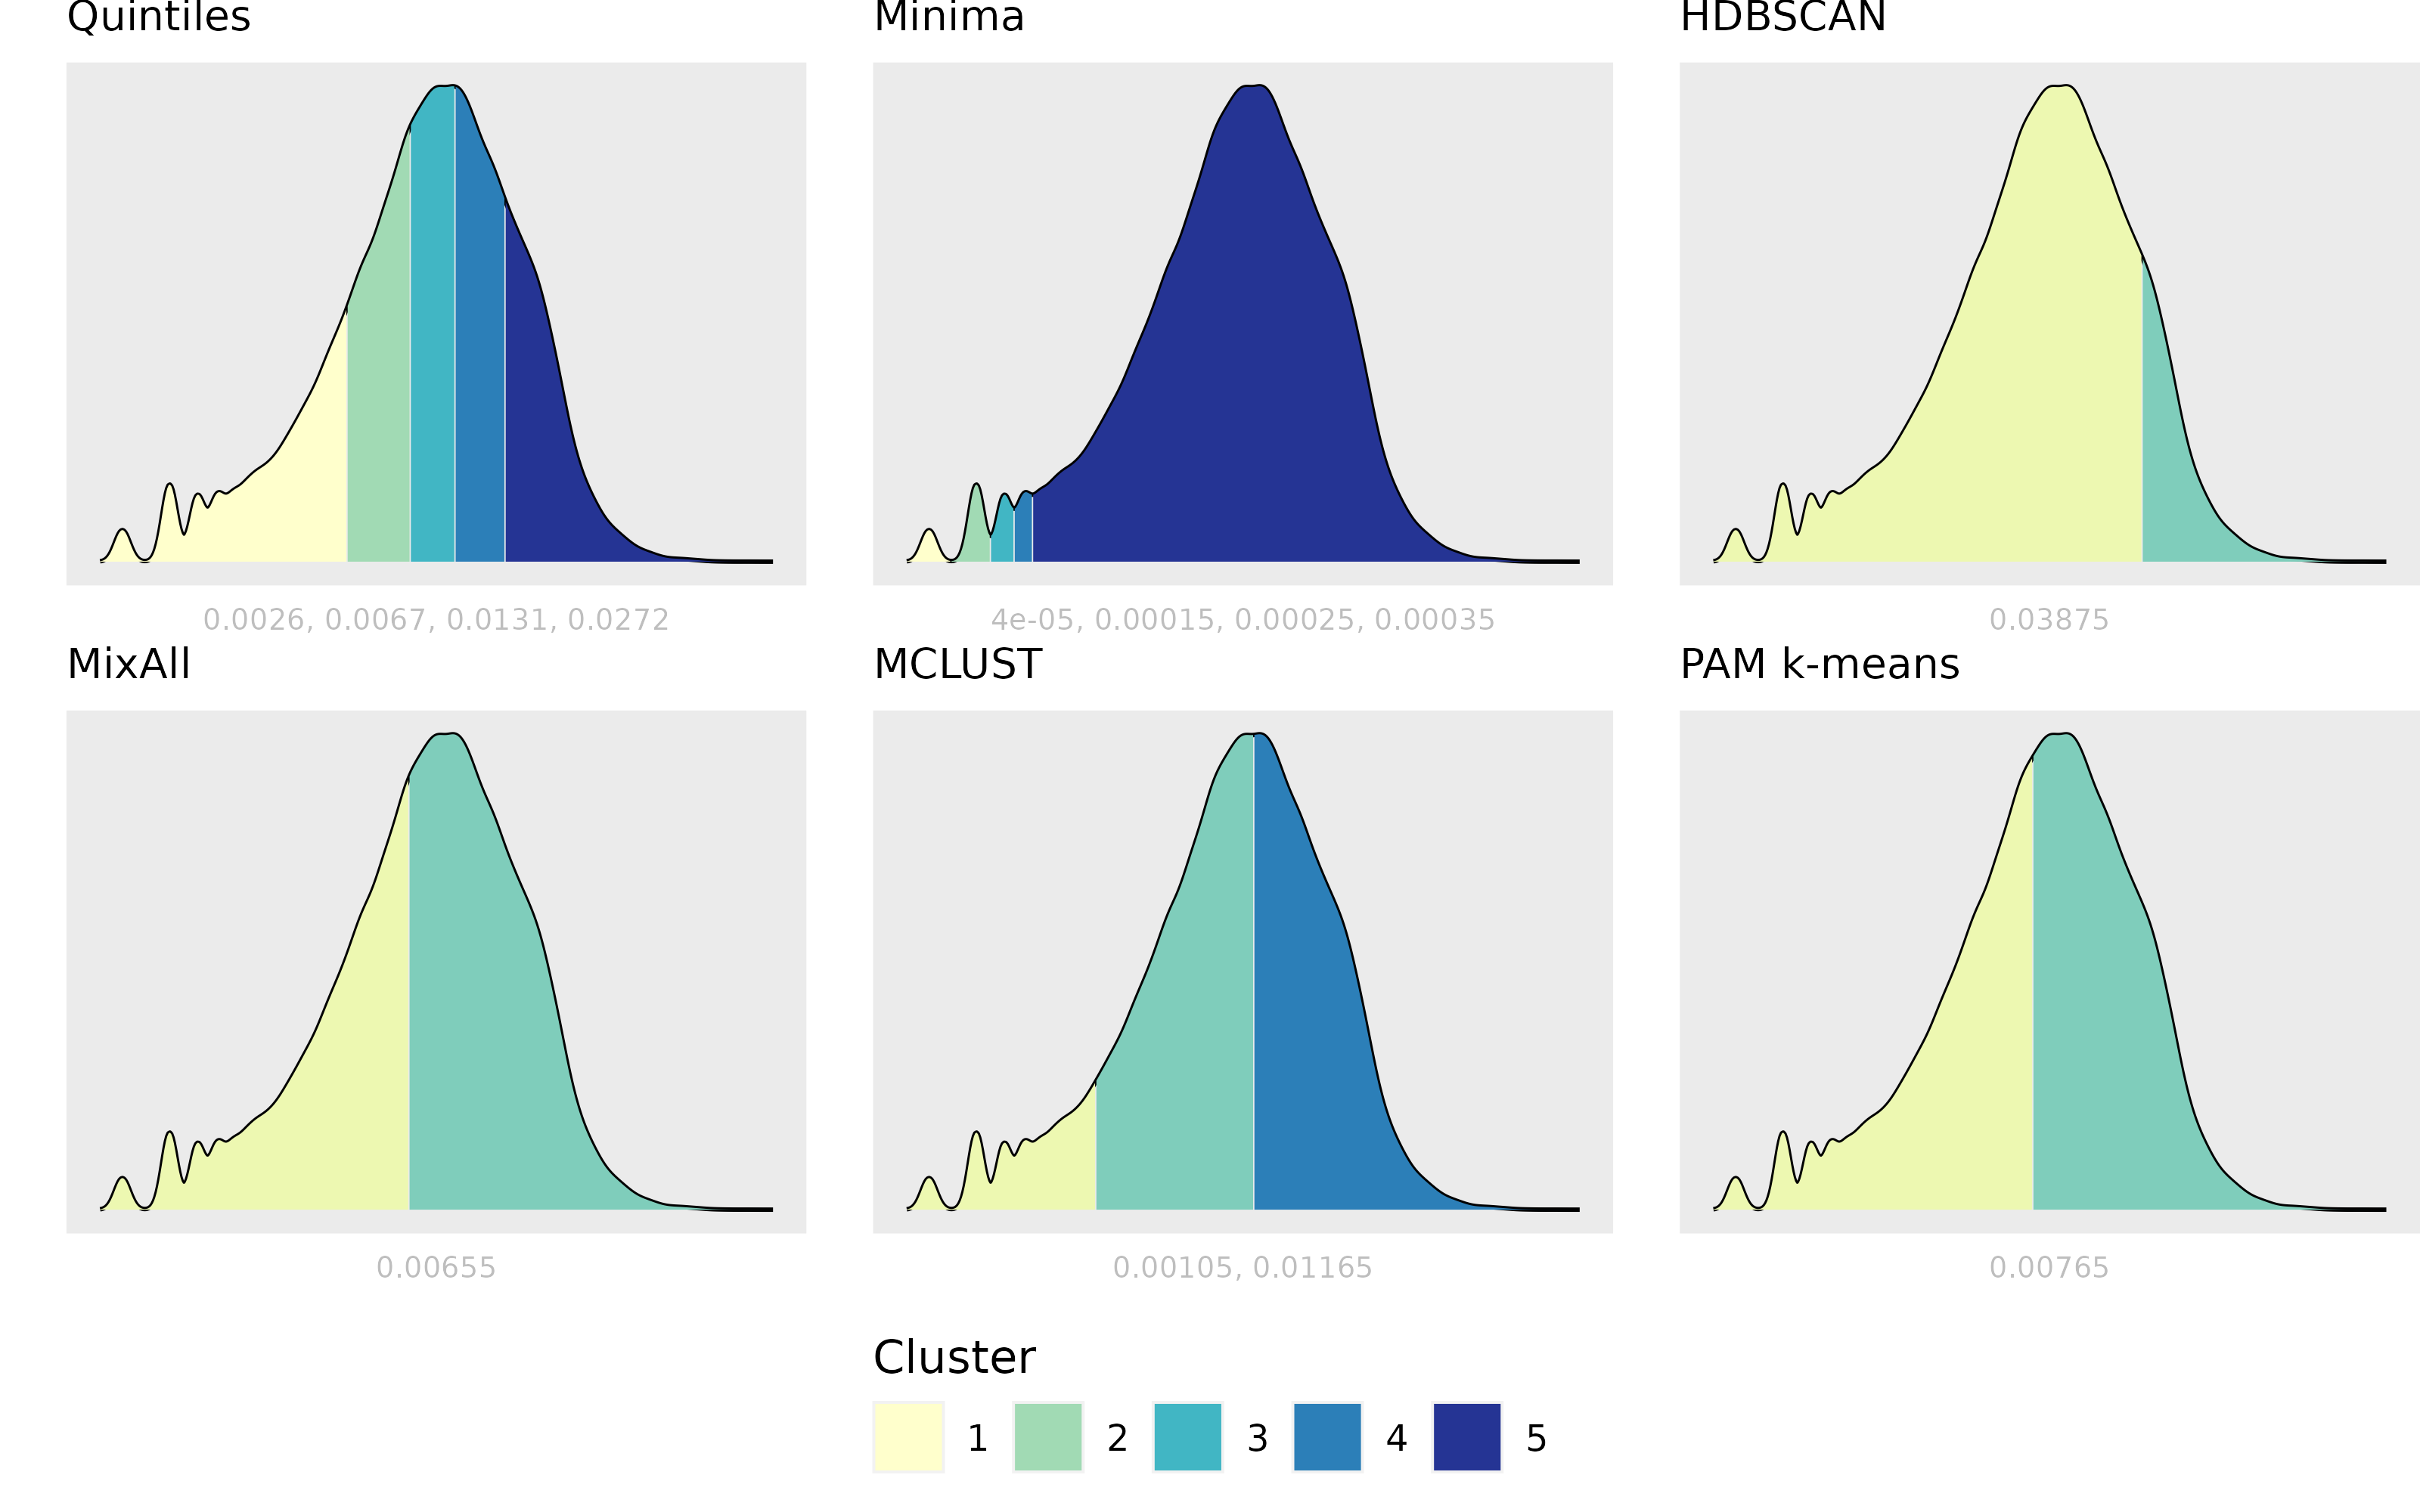
\includegraphics[width=\textwidth]{./cutoffs/by_amenity/Transit_cutoffs.png}
\caption[Transit cutoffs]{Cut-offs values shown on the log-transformed density plots for all clustering approaches transit amenity.}\label{transitcutoffs}
\end{figure}













\begin{figure}[H]
\centering
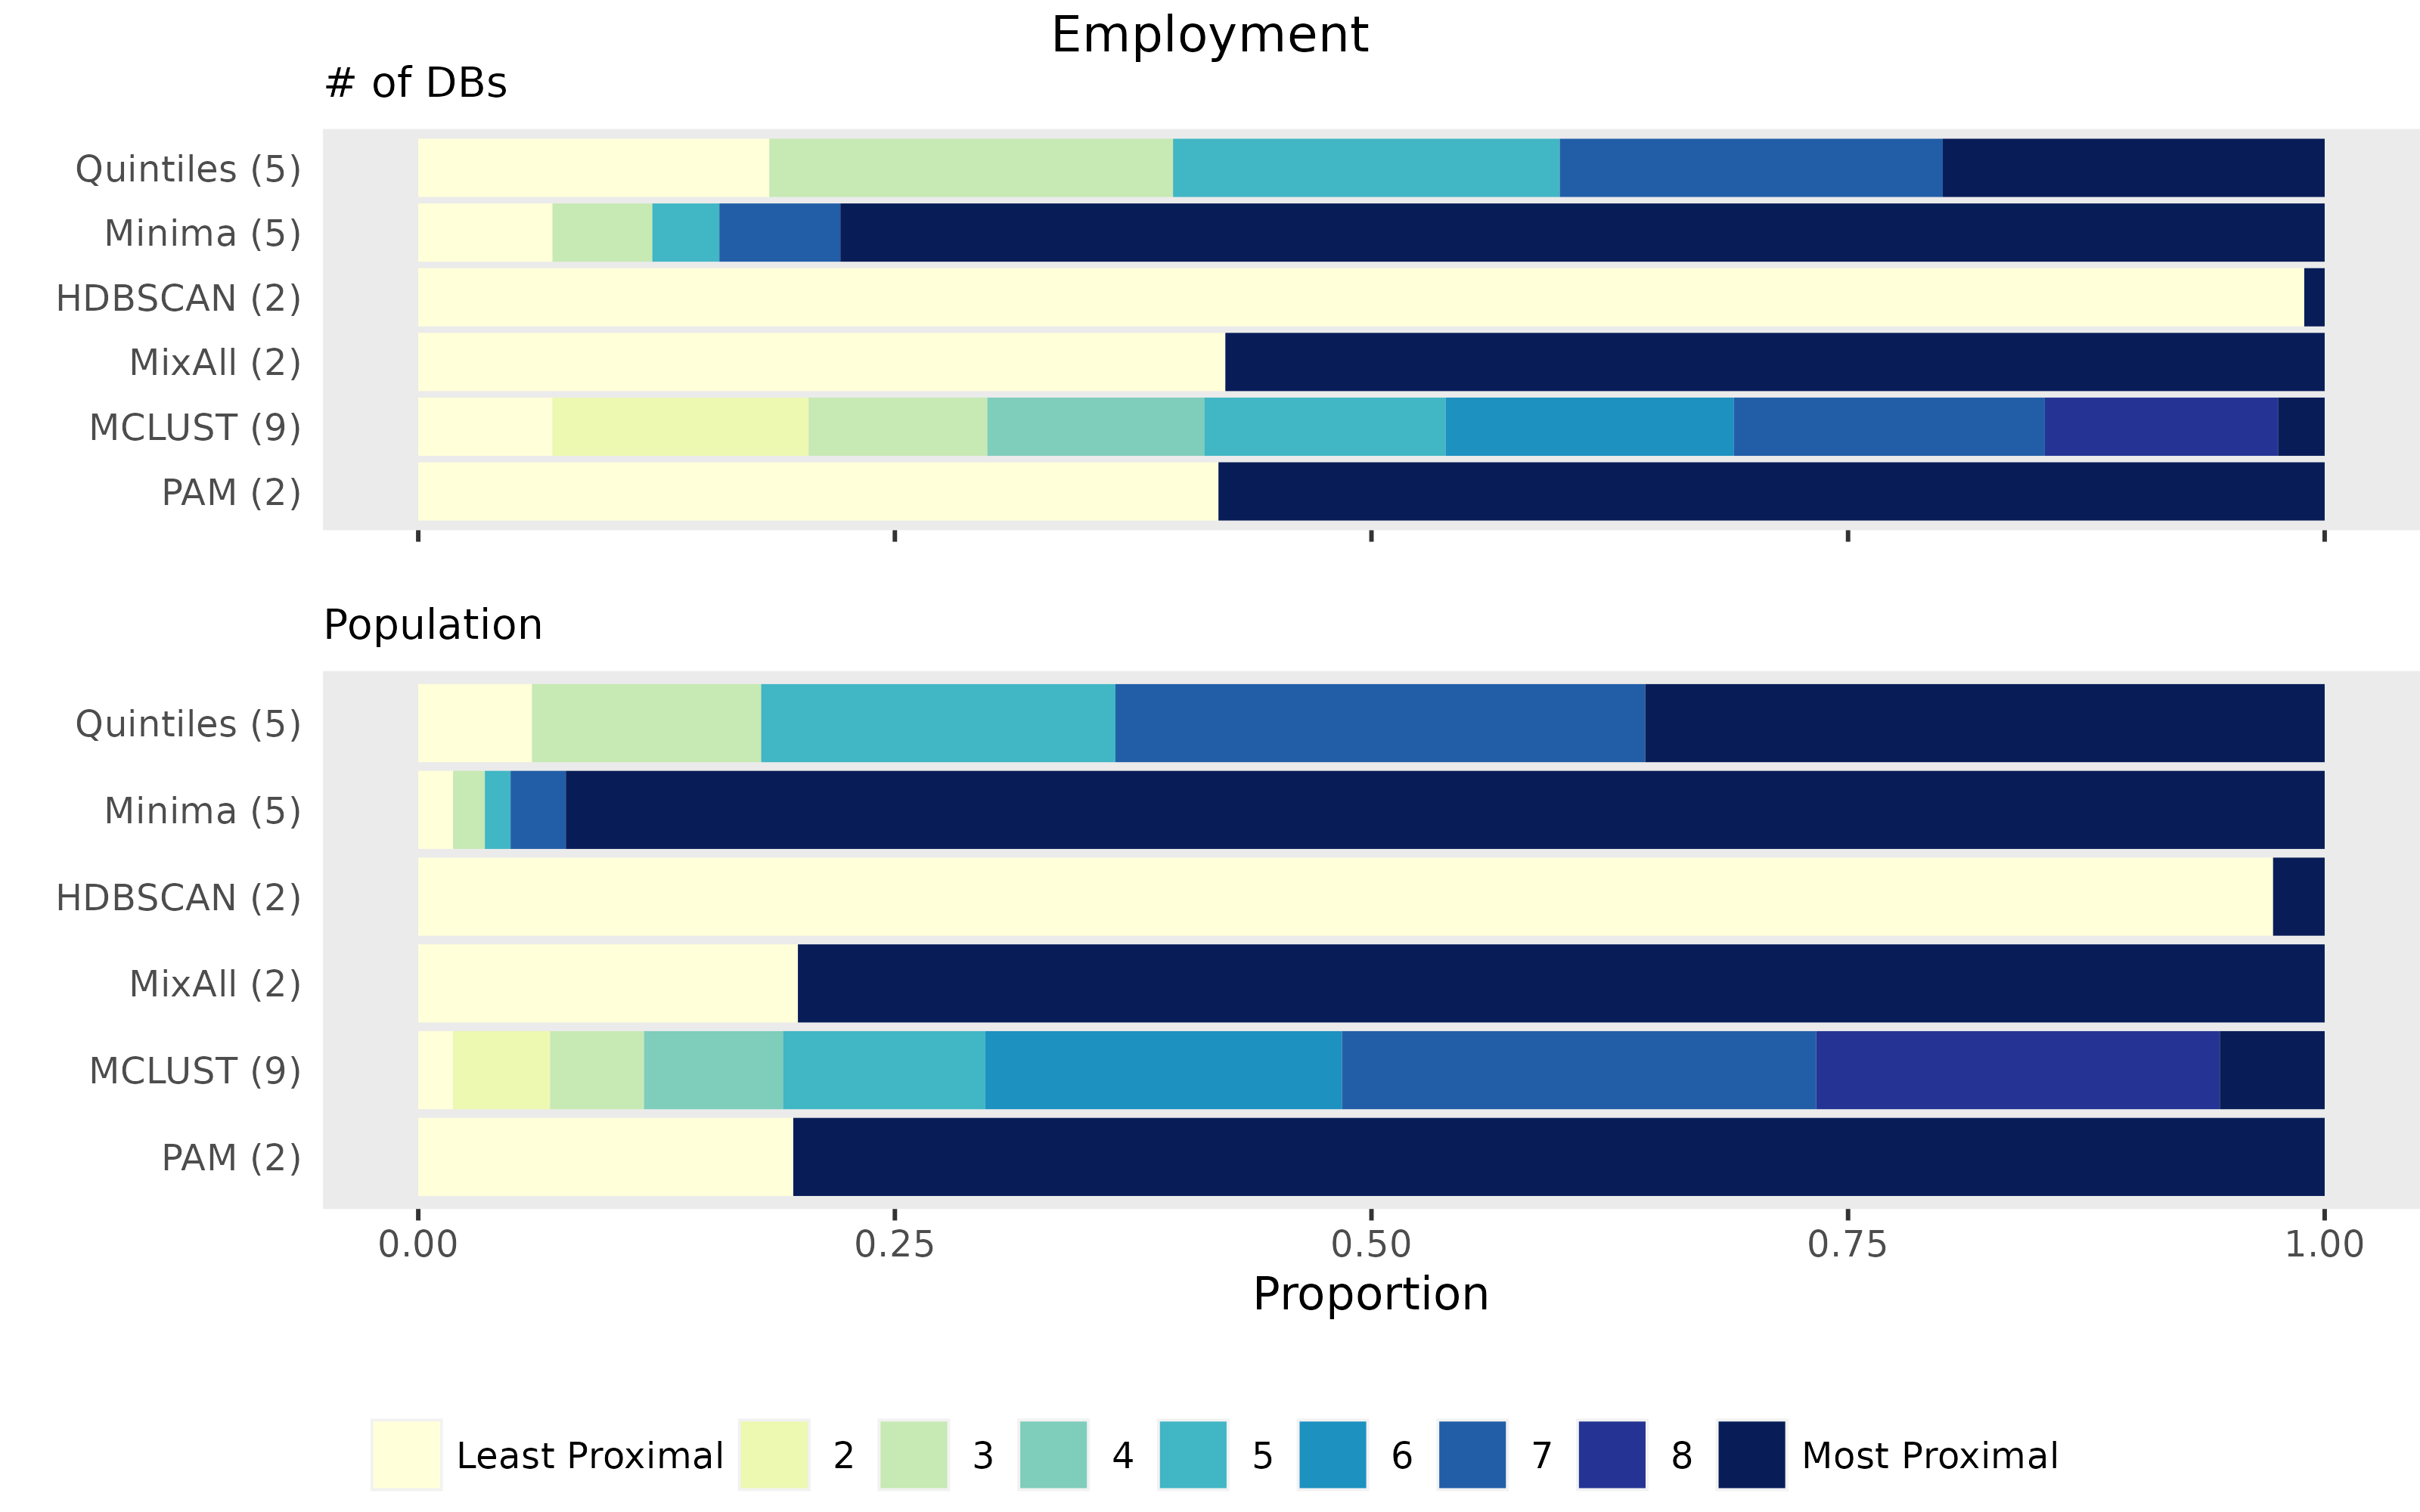
\includegraphics[width=\textwidth]{./barplot_comparison/Employment_barplot.png}
\caption[Employment profile barplot]{Proportion of DBs and population in each cluster for all approaches for the employment amenity.}\label{employmentbarplot}
\end{figure}








\begin{figure}[H]
\centering
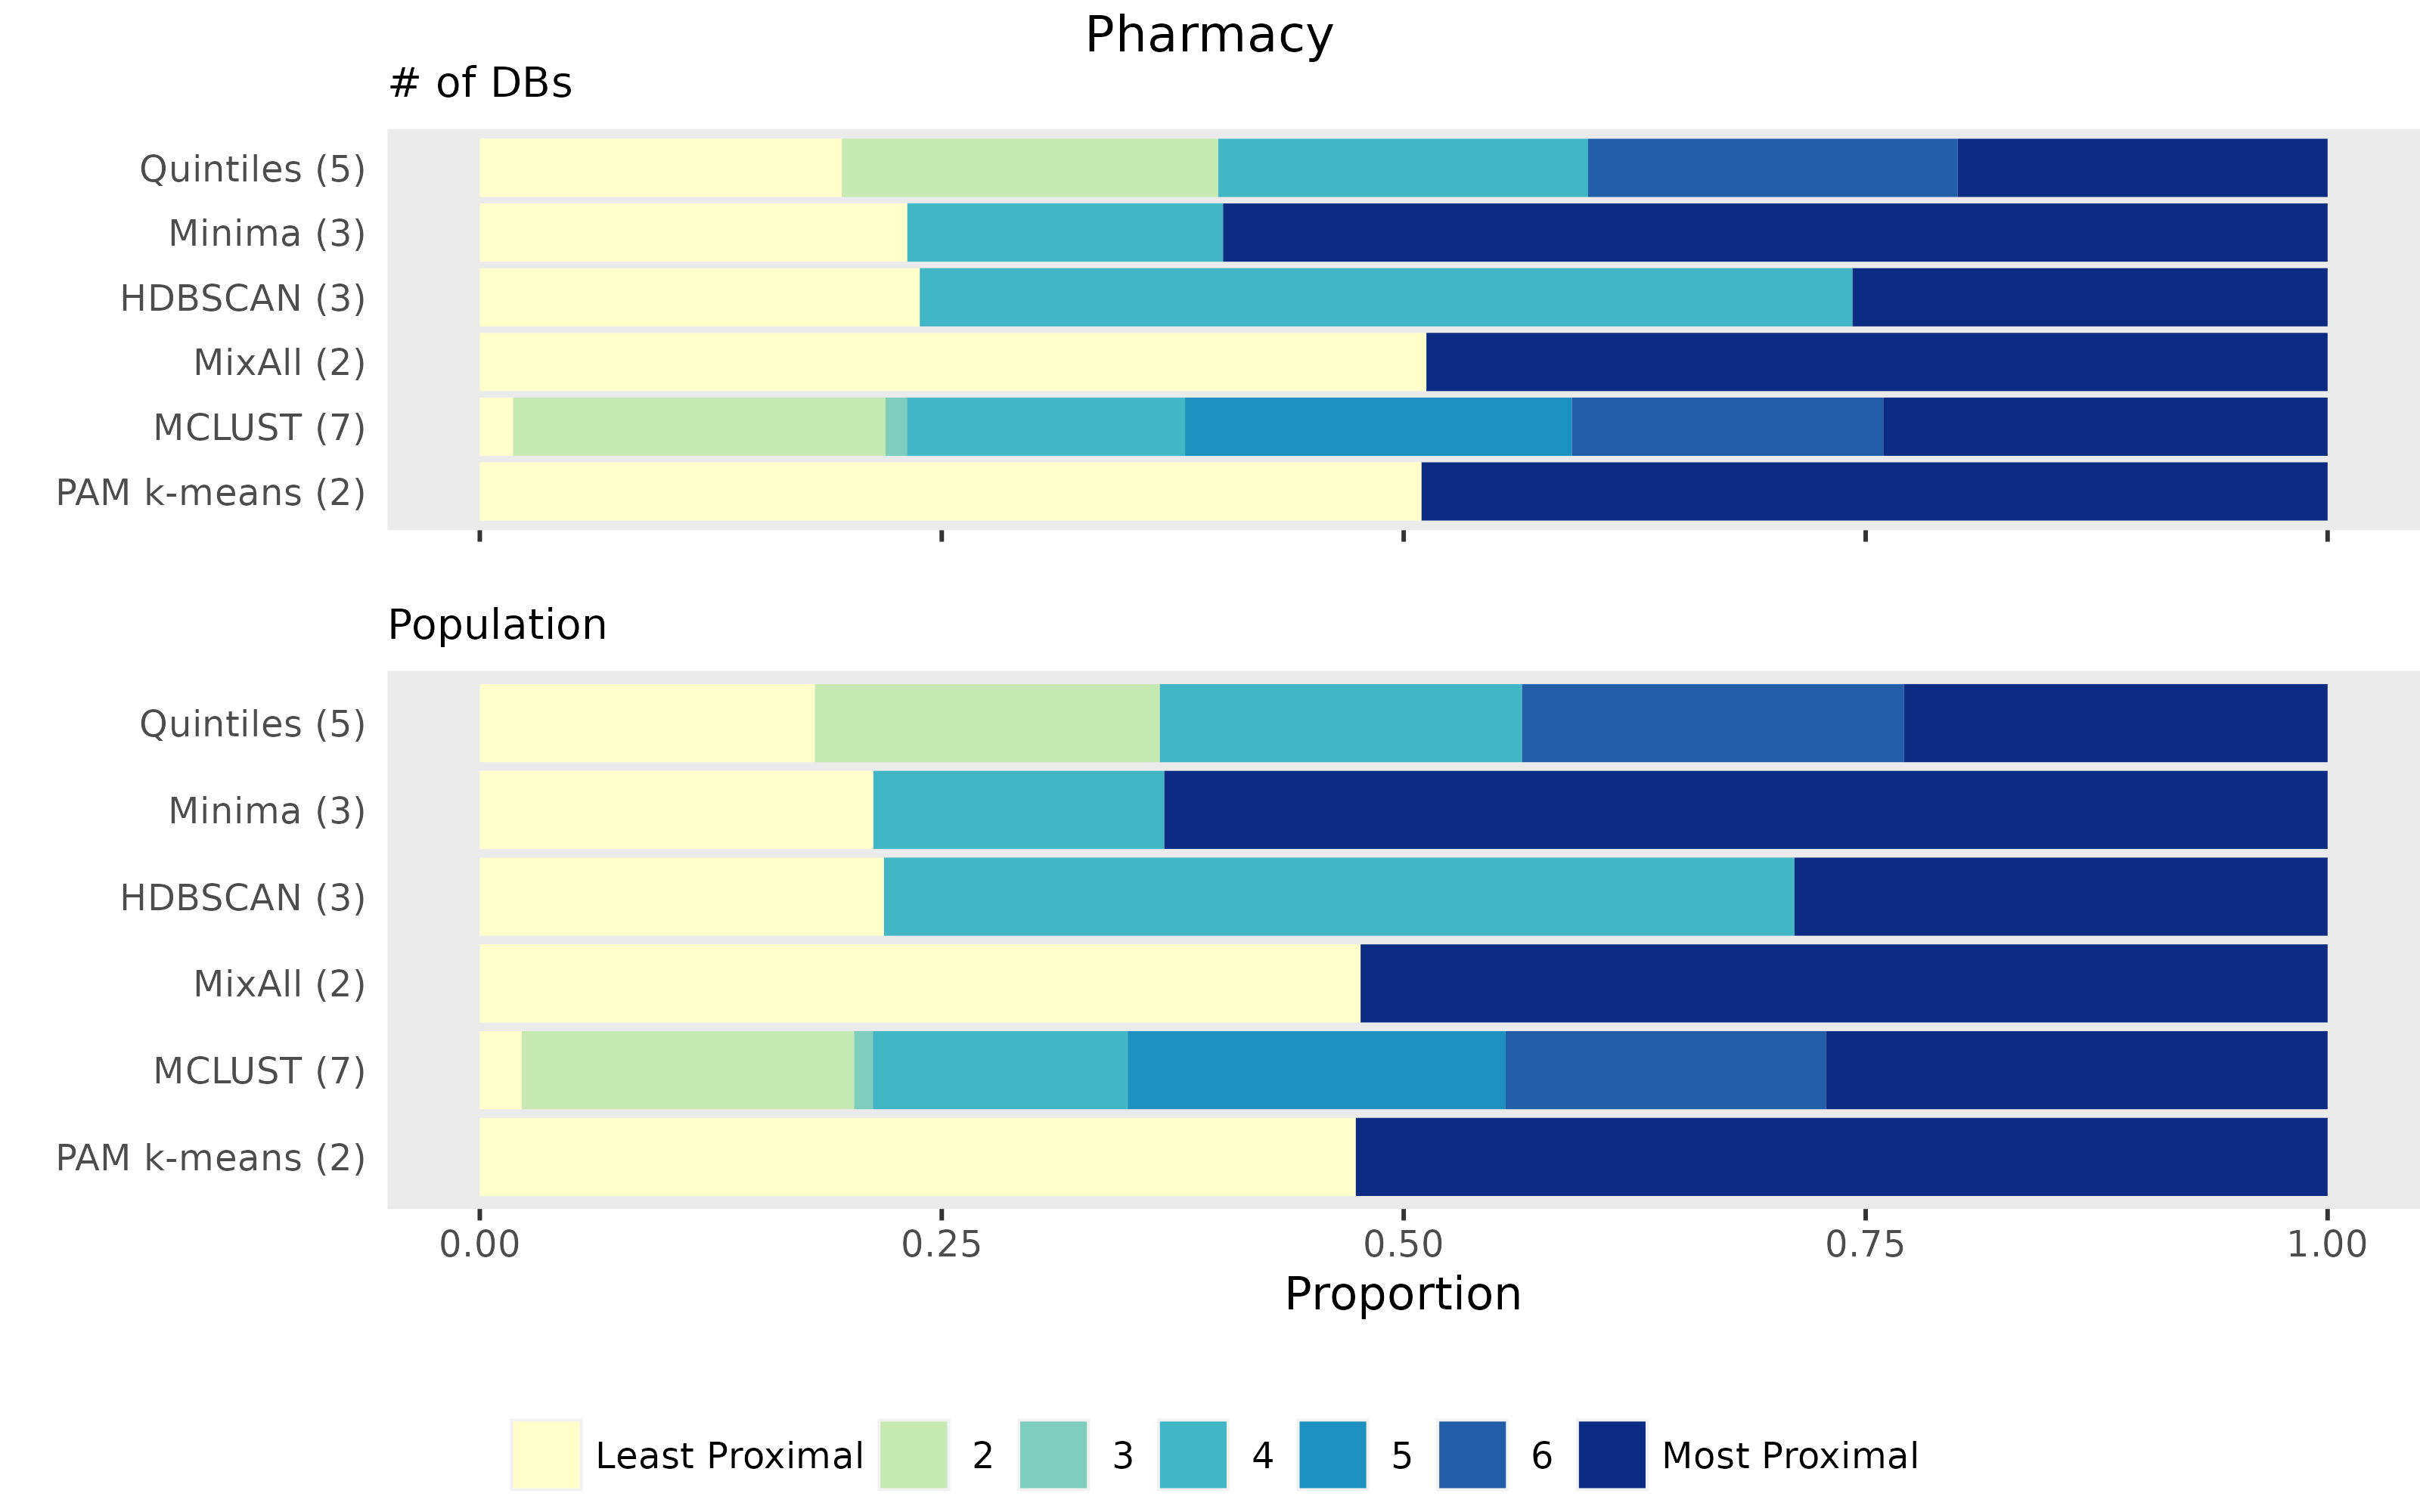
\includegraphics[width=\textwidth]{./barplot_comparison/Pharmacy_barplot.png}
\caption[Pharmacy profile barplot]{Proportion of DBs and population in each cluster for all approaches for the pharmacy amenity.}\label{pharmacybarplot}
\end{figure}









\begin{figure}[H]
\centering
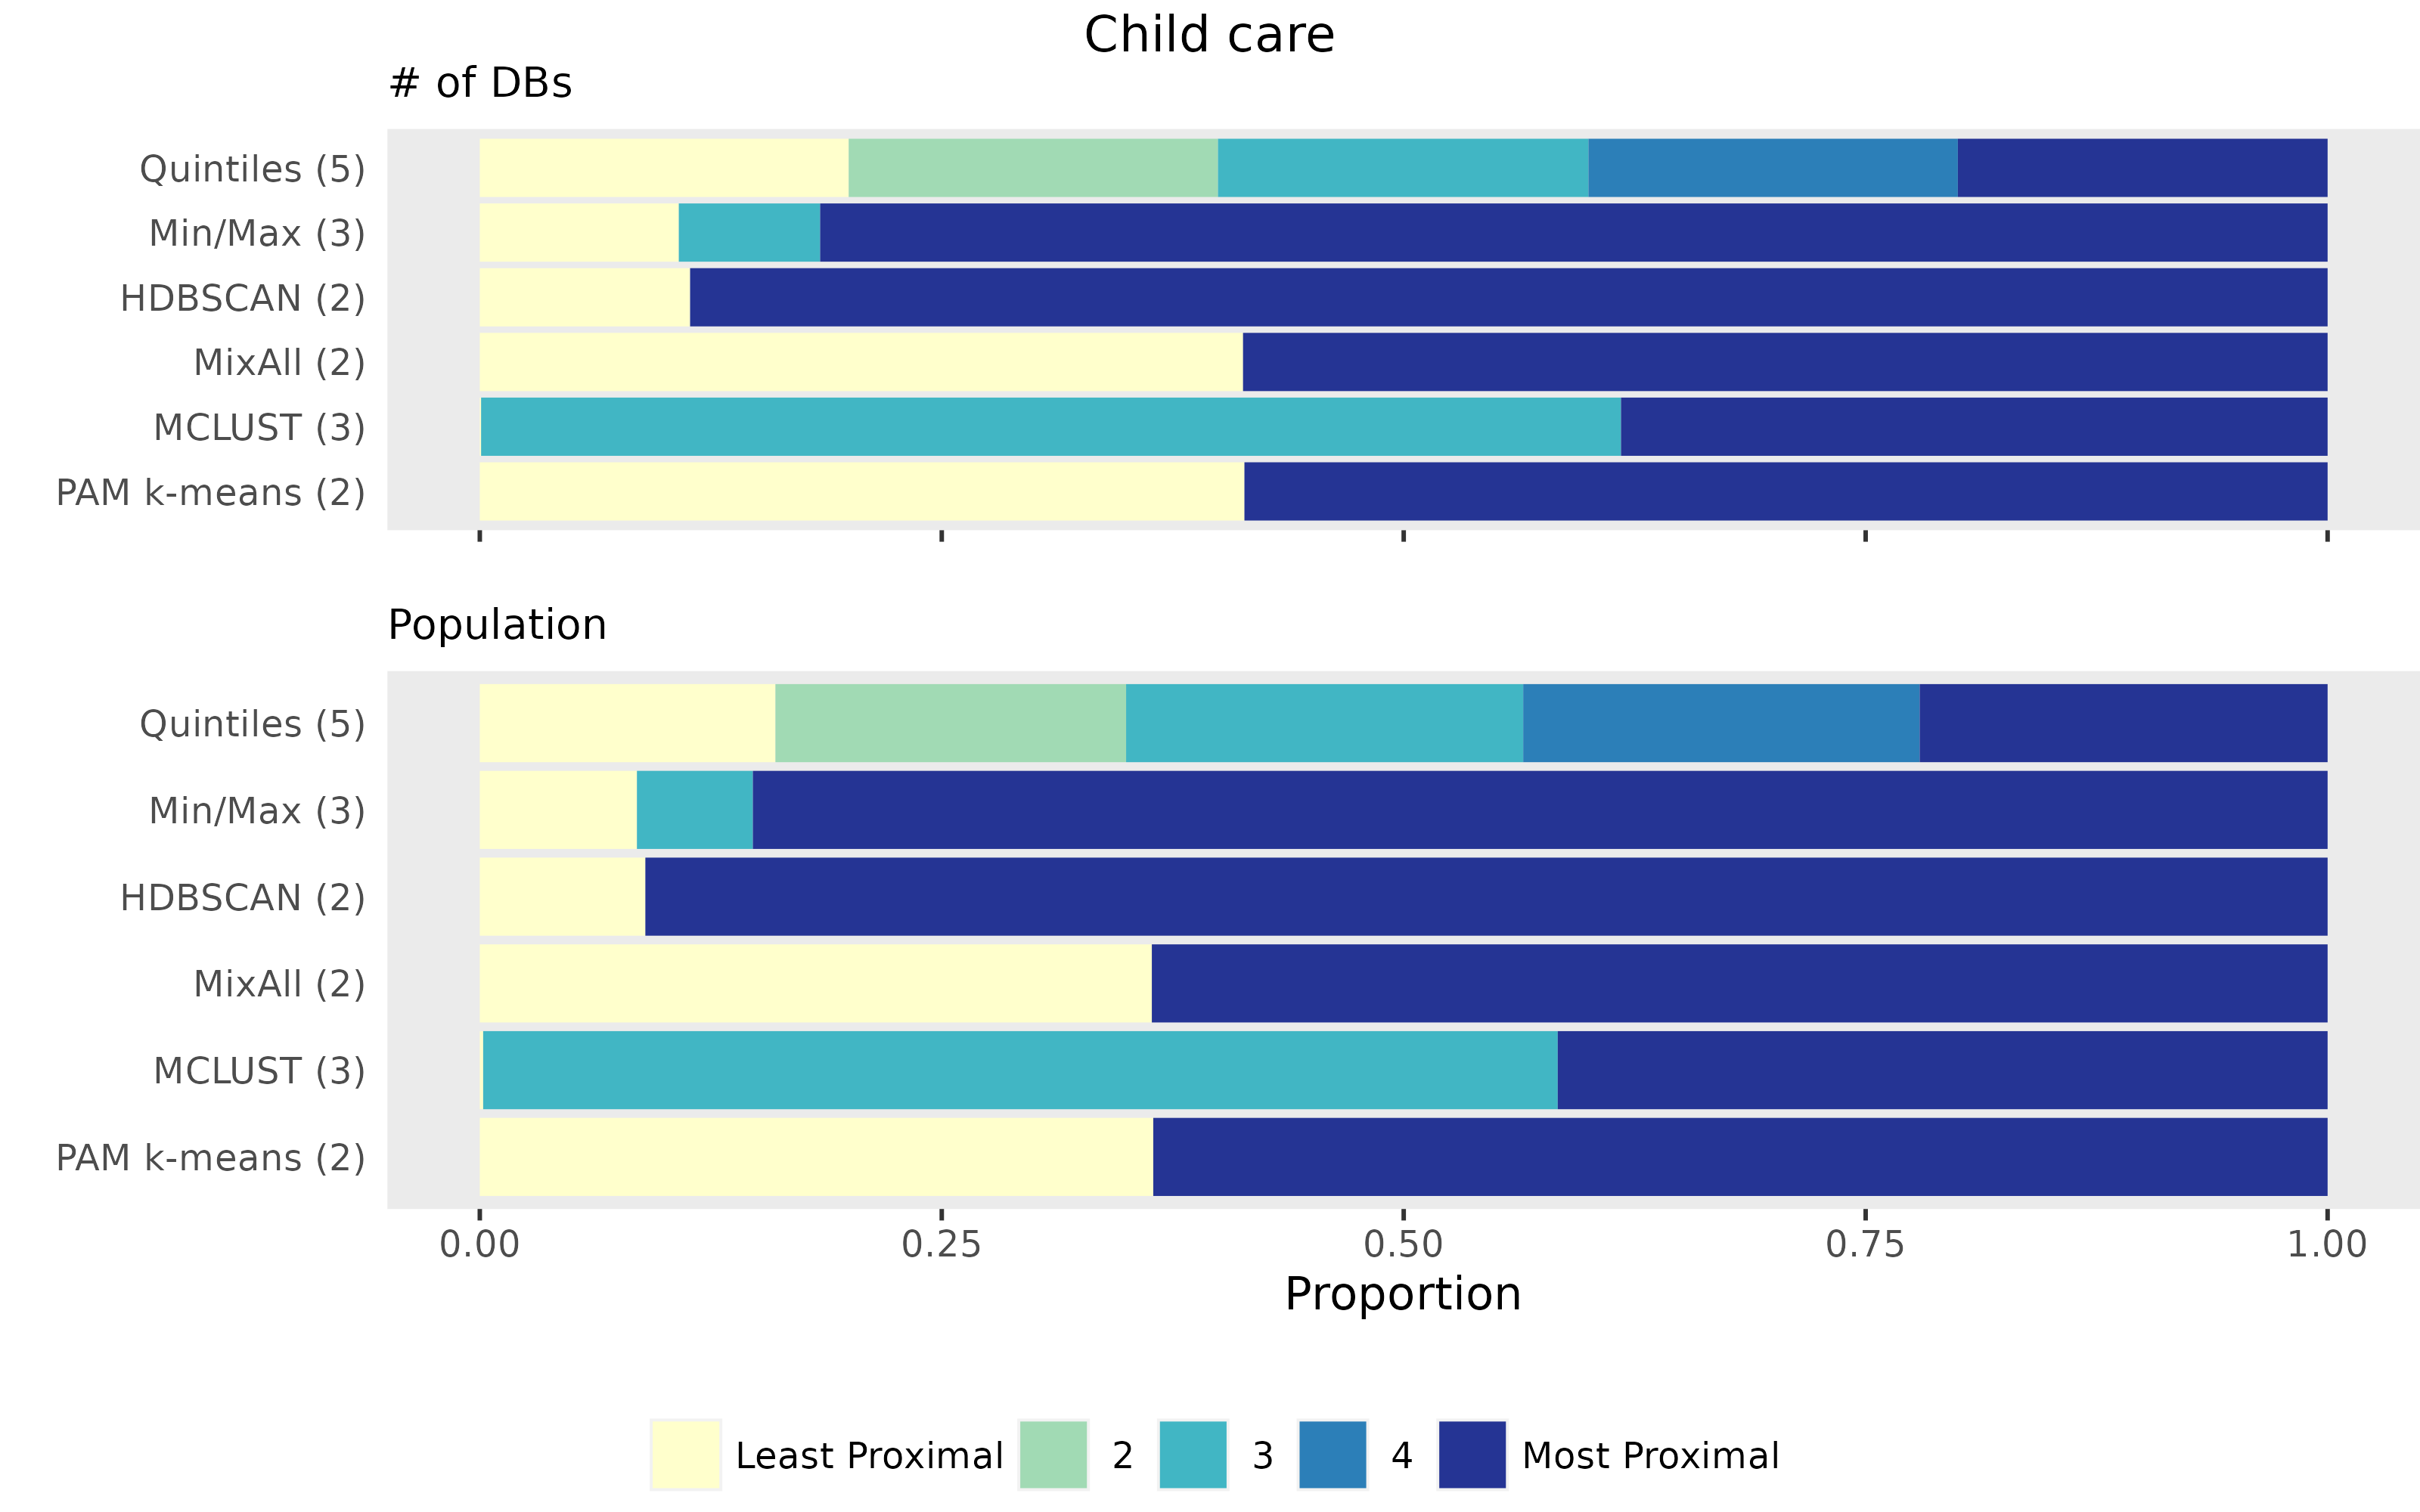
\includegraphics[width=\textwidth]{./barplot_comparison/Child care_barplot.png}
\caption[Child care profile barplot]{Proportion of DBs and population in each cluster for all approaches for the child care amenity.}\label{childcarebarplot}
\end{figure}









\begin{figure}[H]
\centering
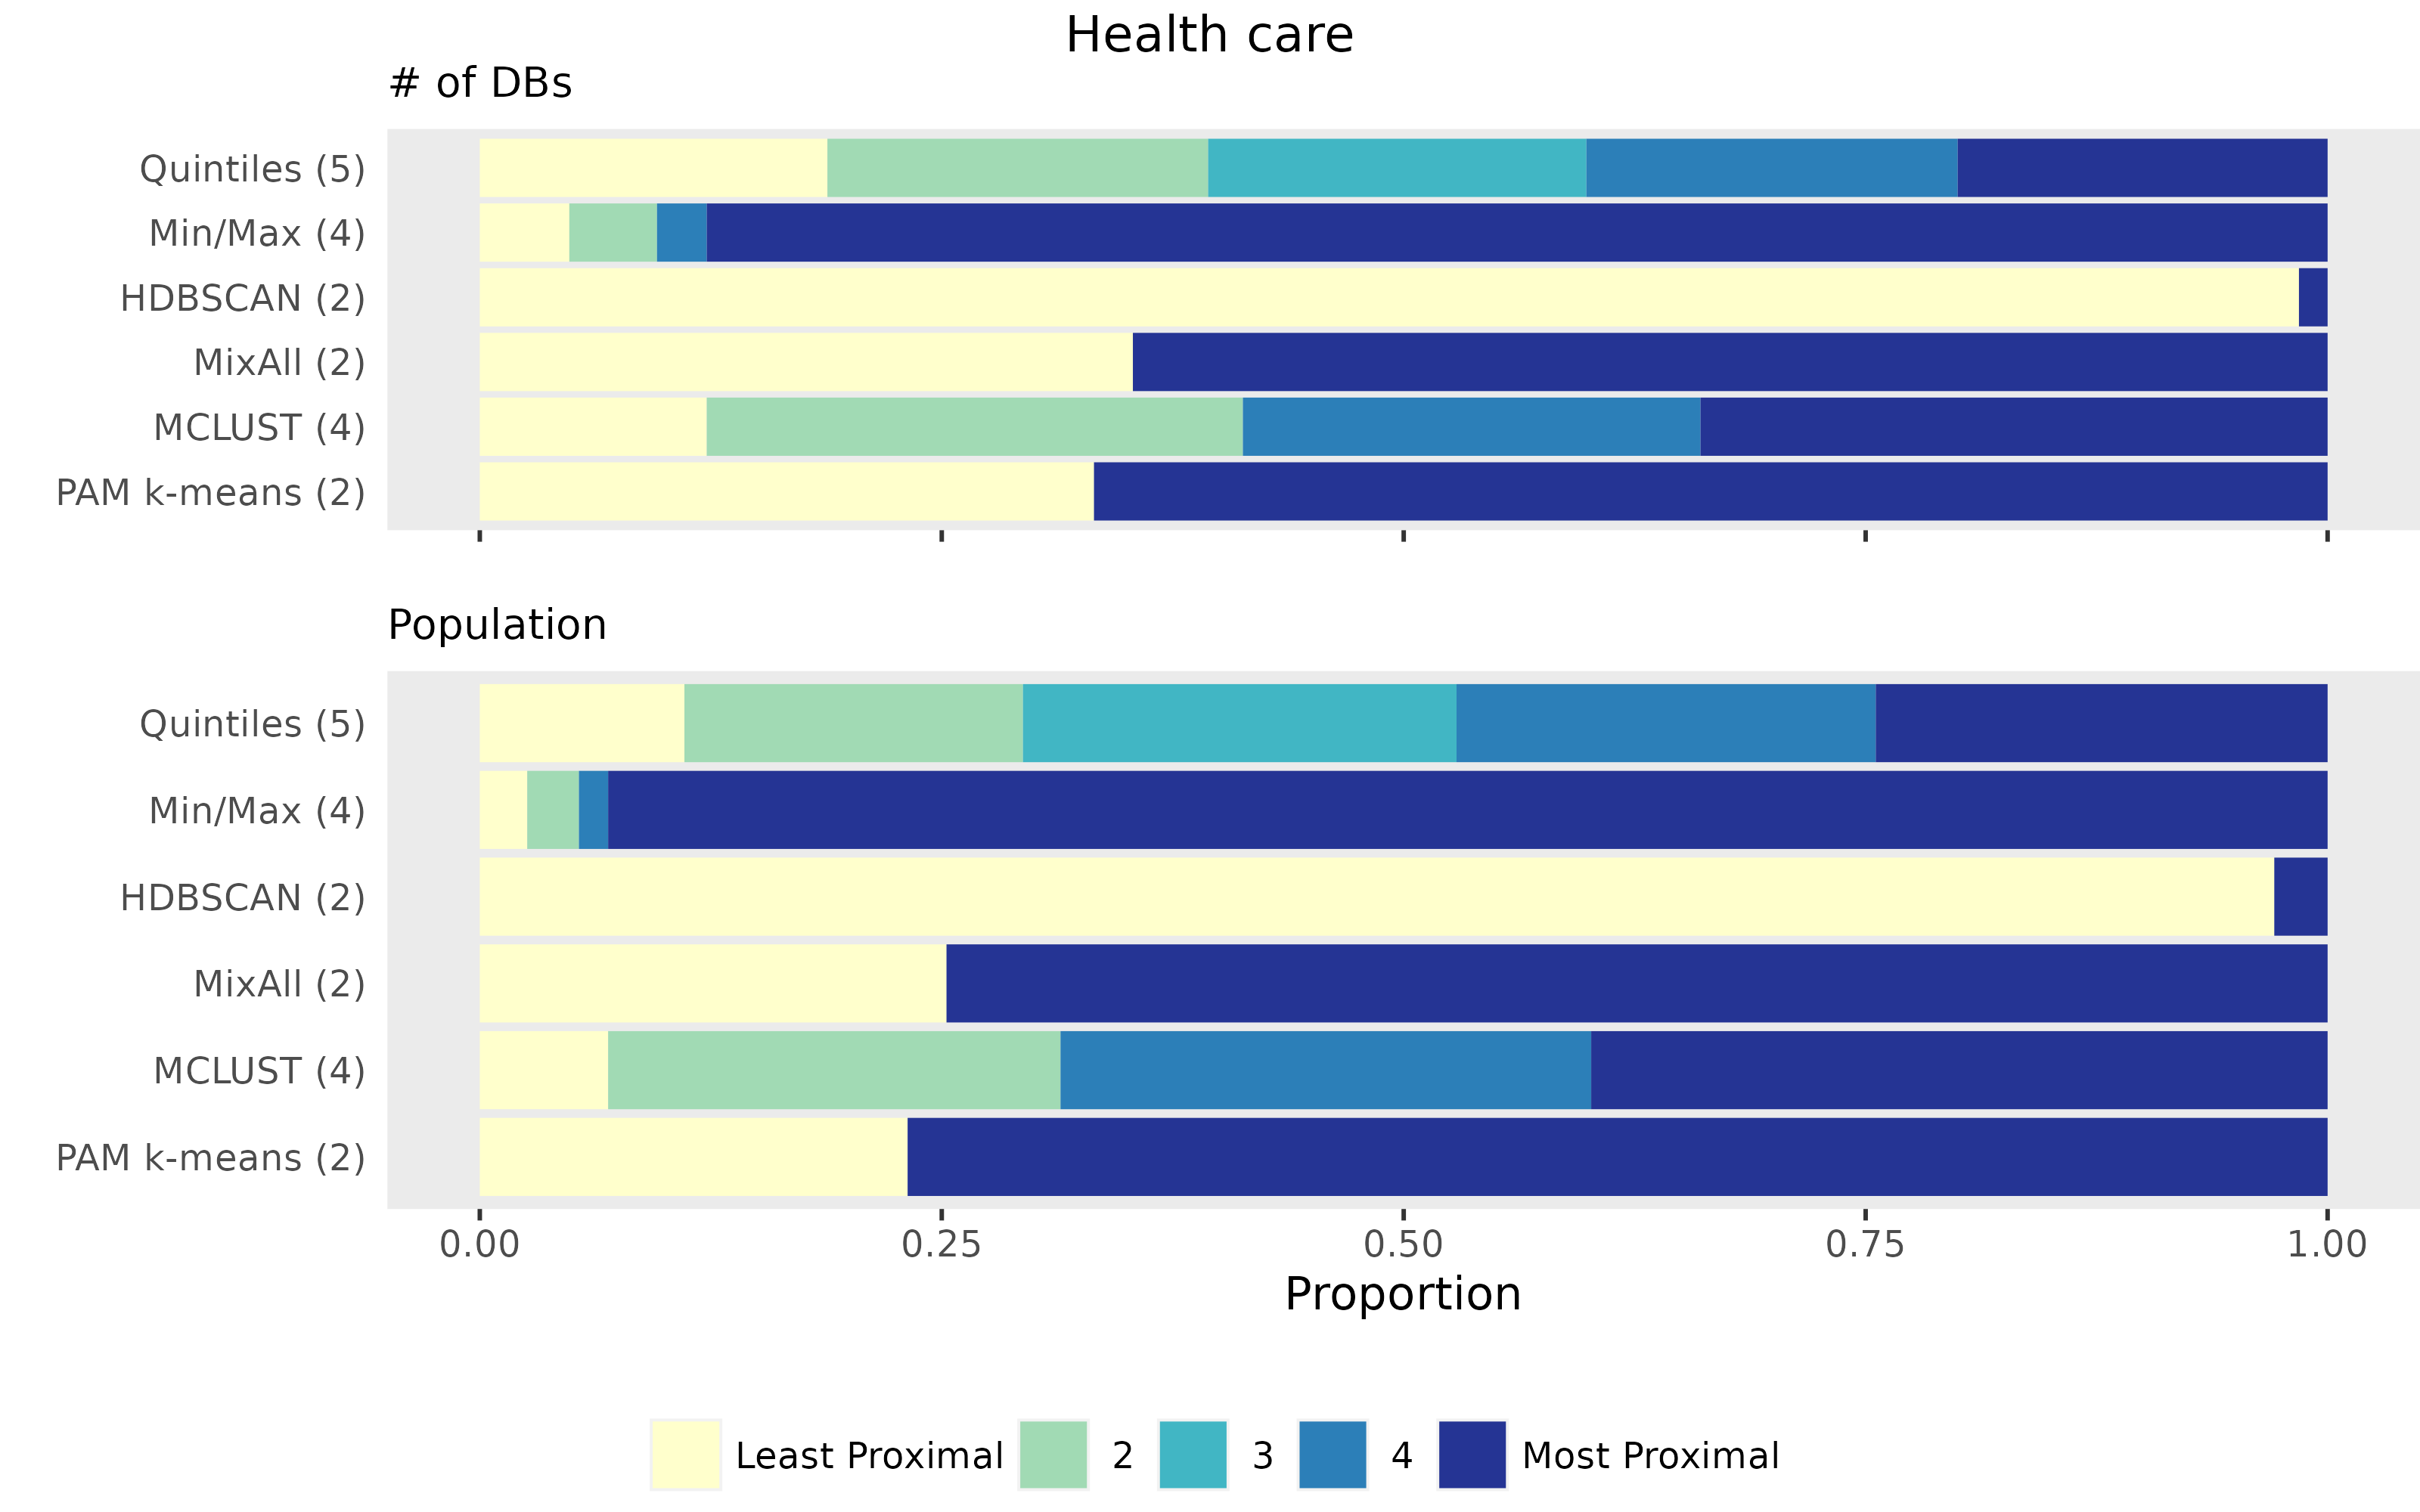
\includegraphics[width=\textwidth]{./barplot_comparison/Health care_barplot.png}
\caption[Health care profile barplot]{Proportion of DBs and population in each cluster for all approaches for the health care amenity.}\label{healthcarebarplot}
\end{figure}









\begin{figure}[H]
\centering
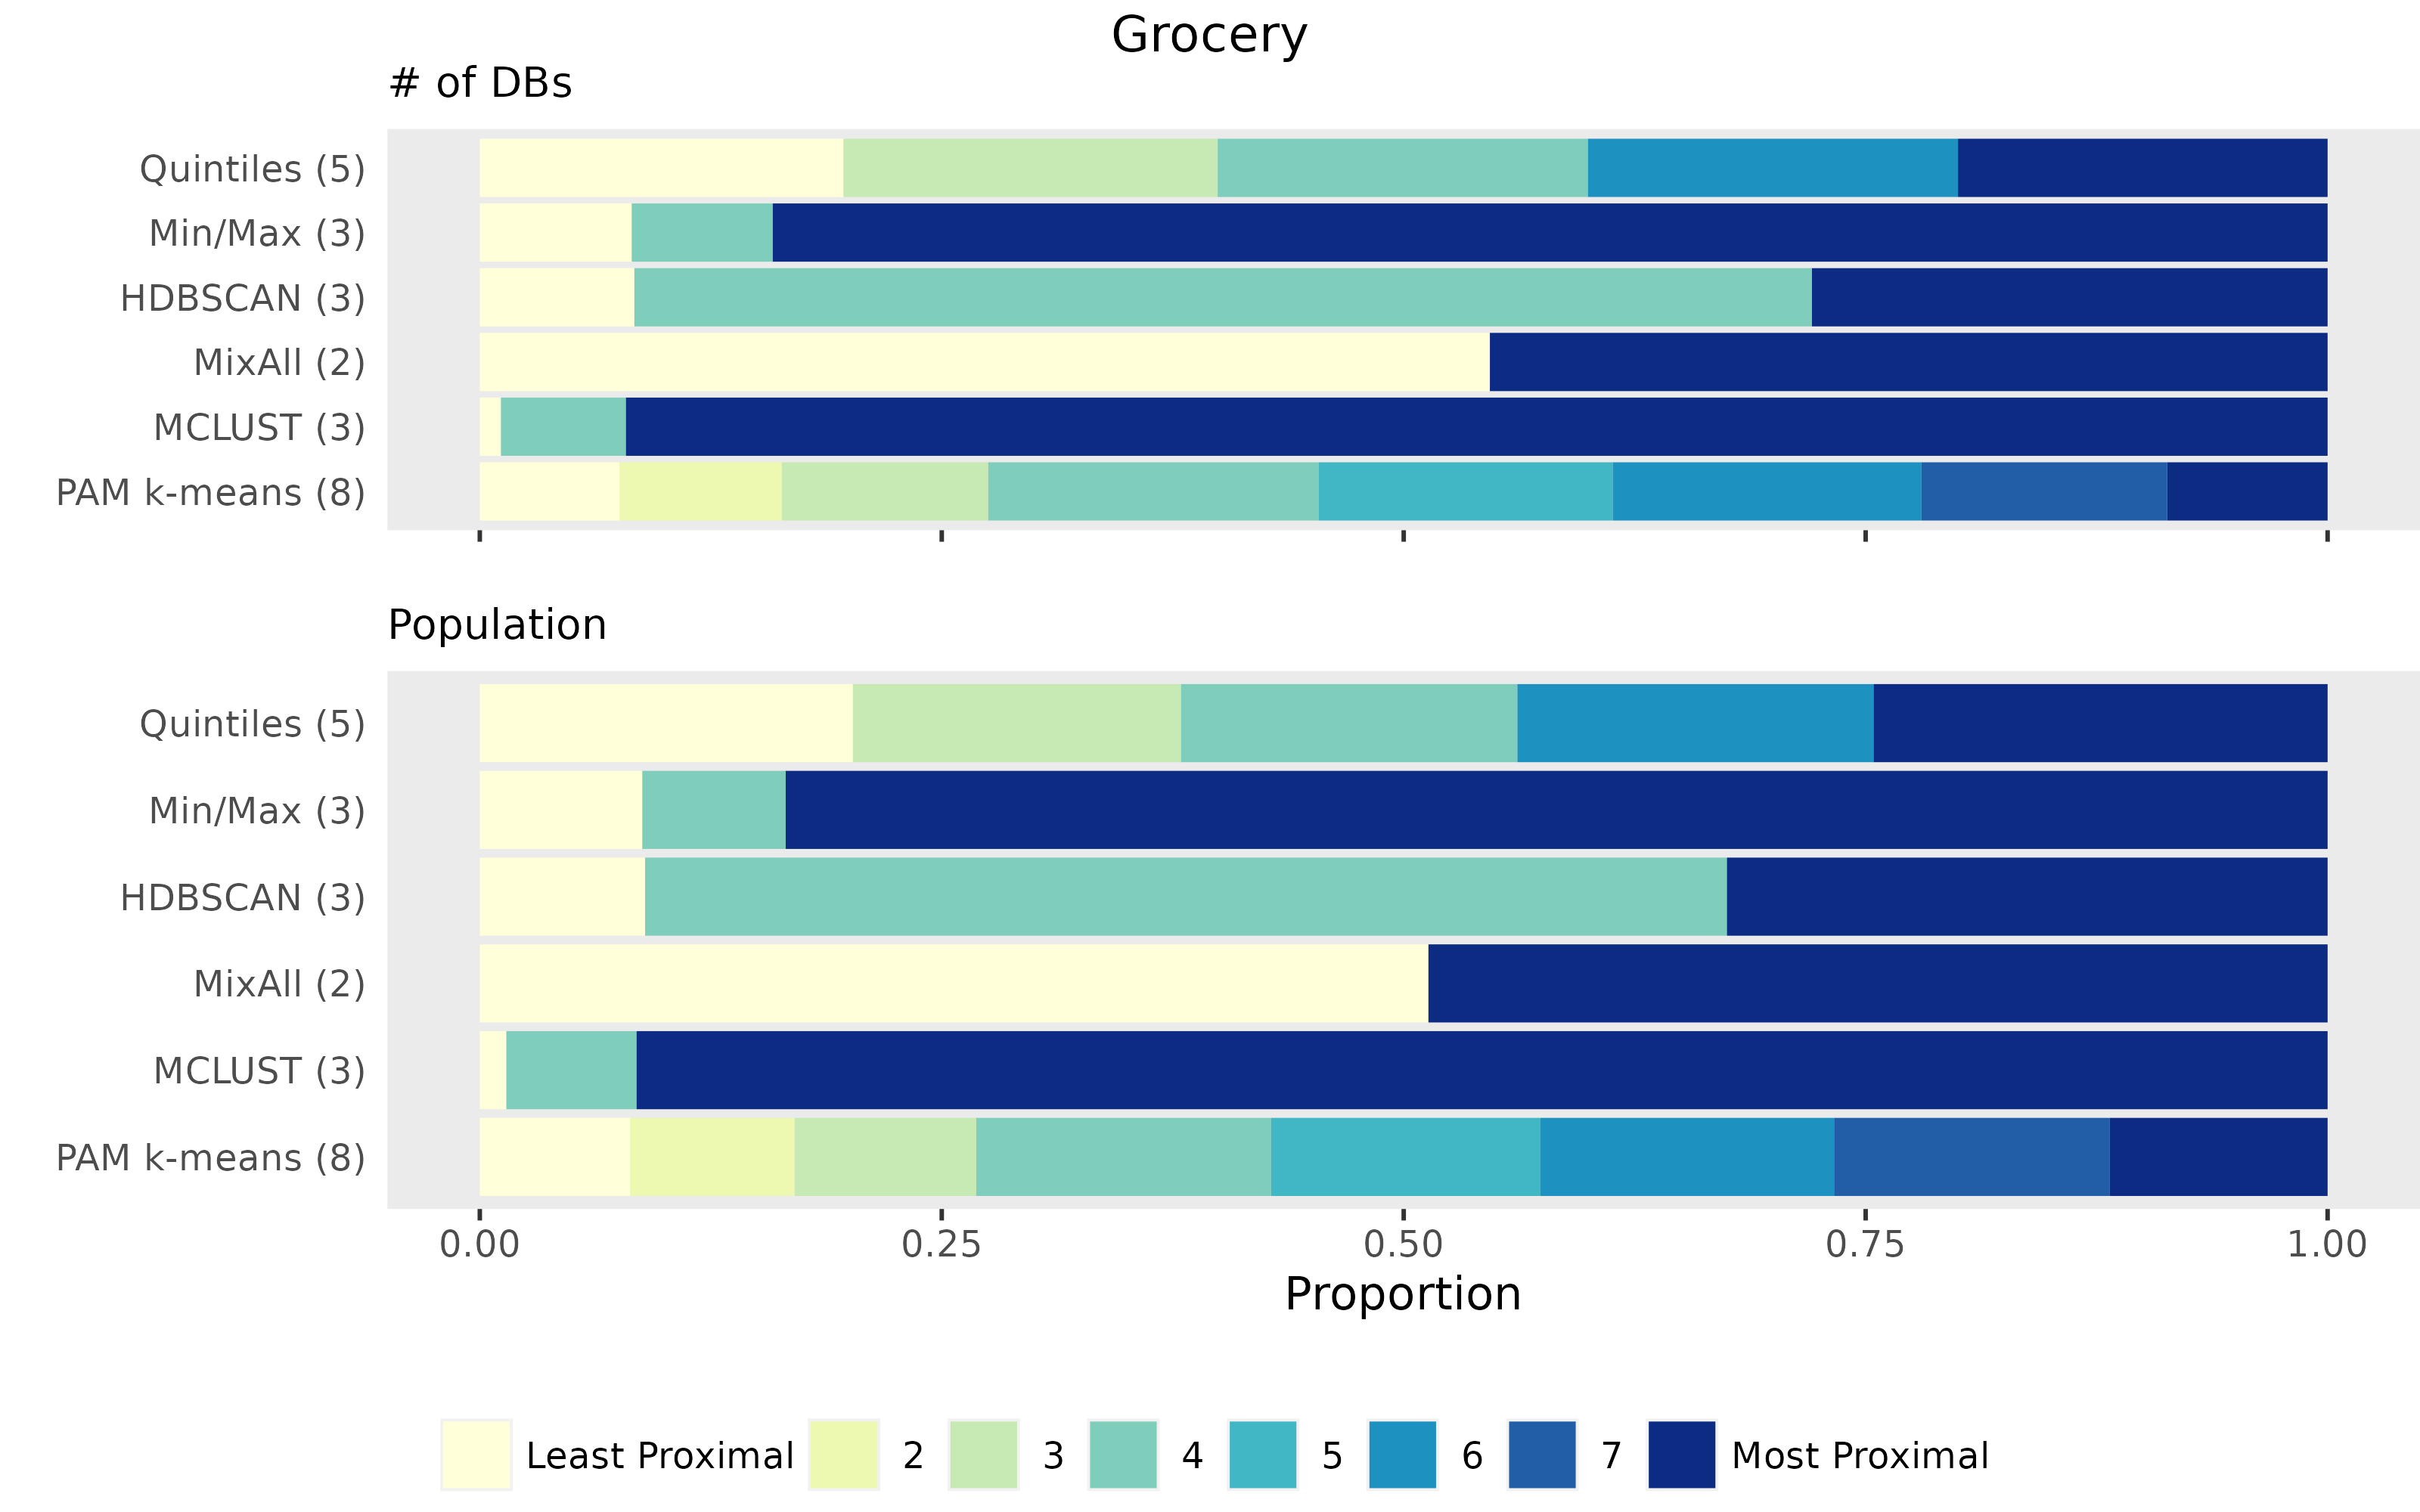
\includegraphics[width=\textwidth]{./barplot_comparison/Grocery_barplot.png}
\caption[Grocery profile barplot]{Proportion of DBs and population in each cluster for all approaches for the grocery amenity.}\label{grocerybarplot}
\end{figure}









\begin{figure}[H]
\centering
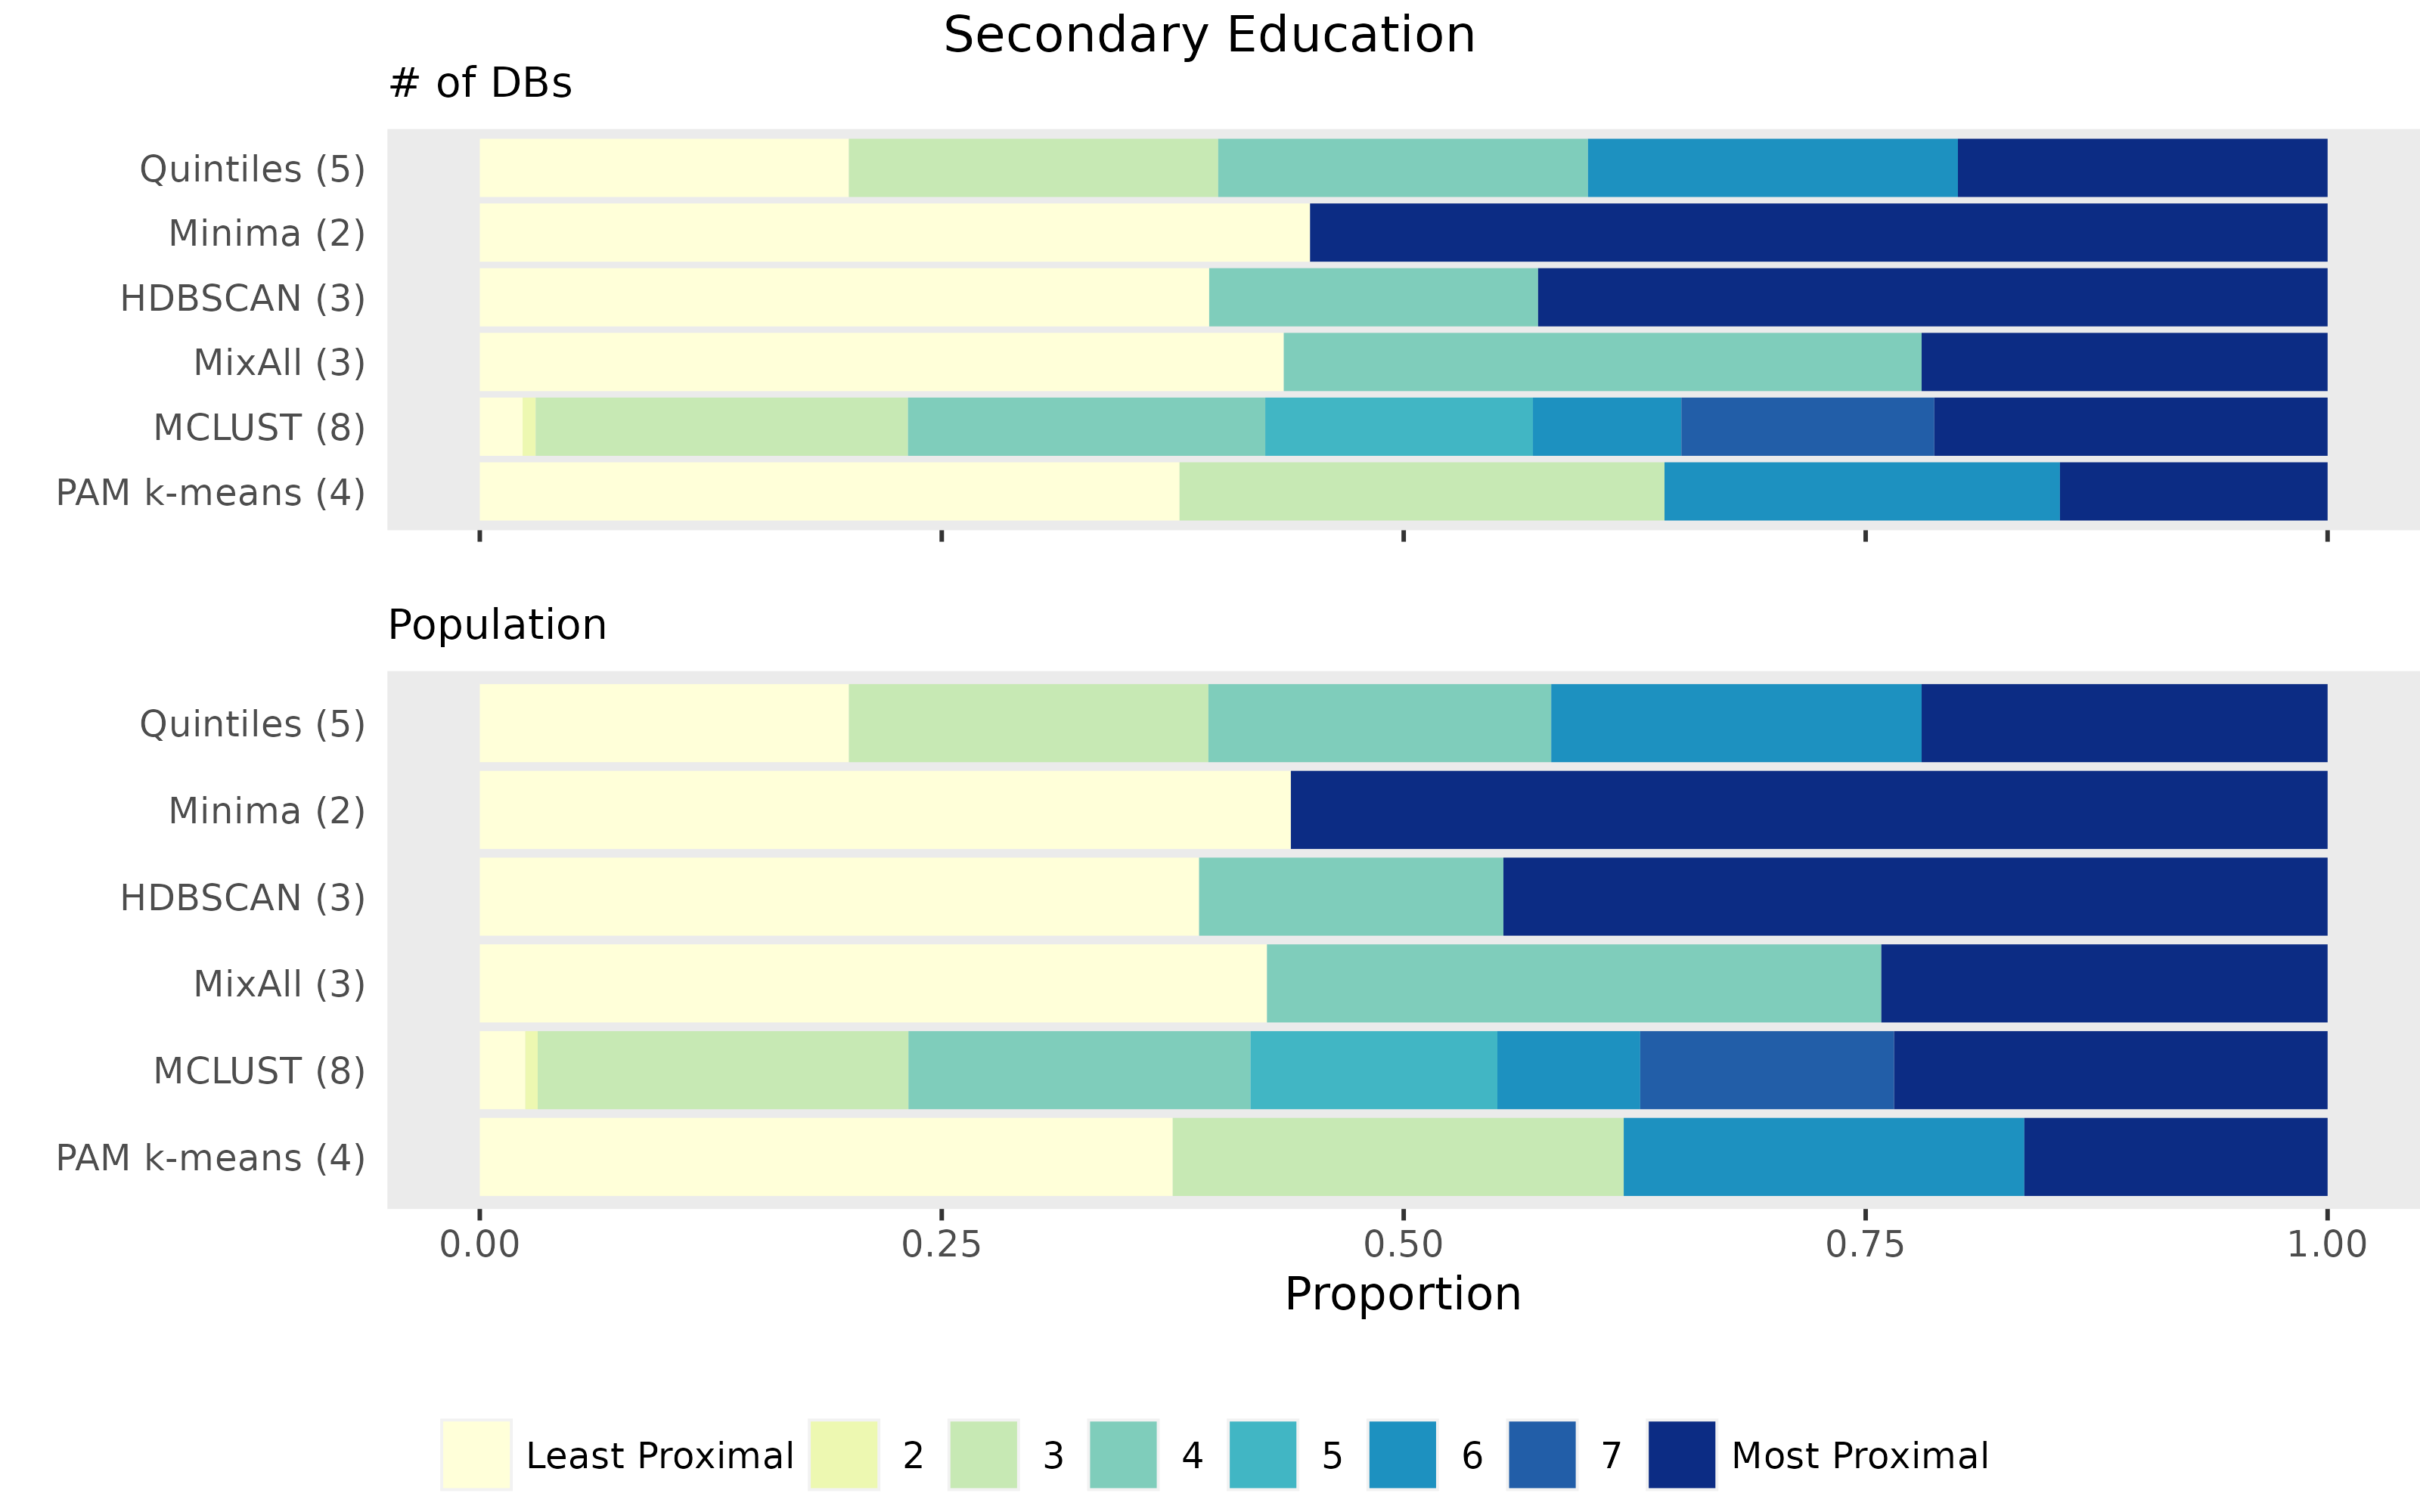
\includegraphics[width=\textwidth]{./barplot_comparison/Secondary Education_barplot.png}
\caption[Secondary education profile barplot]{Proportion of DBs and population in each cluster for all approaches for the secondary education amenity.}\label{seceducbarplot}
\end{figure}









\begin{figure}[H]
\centering
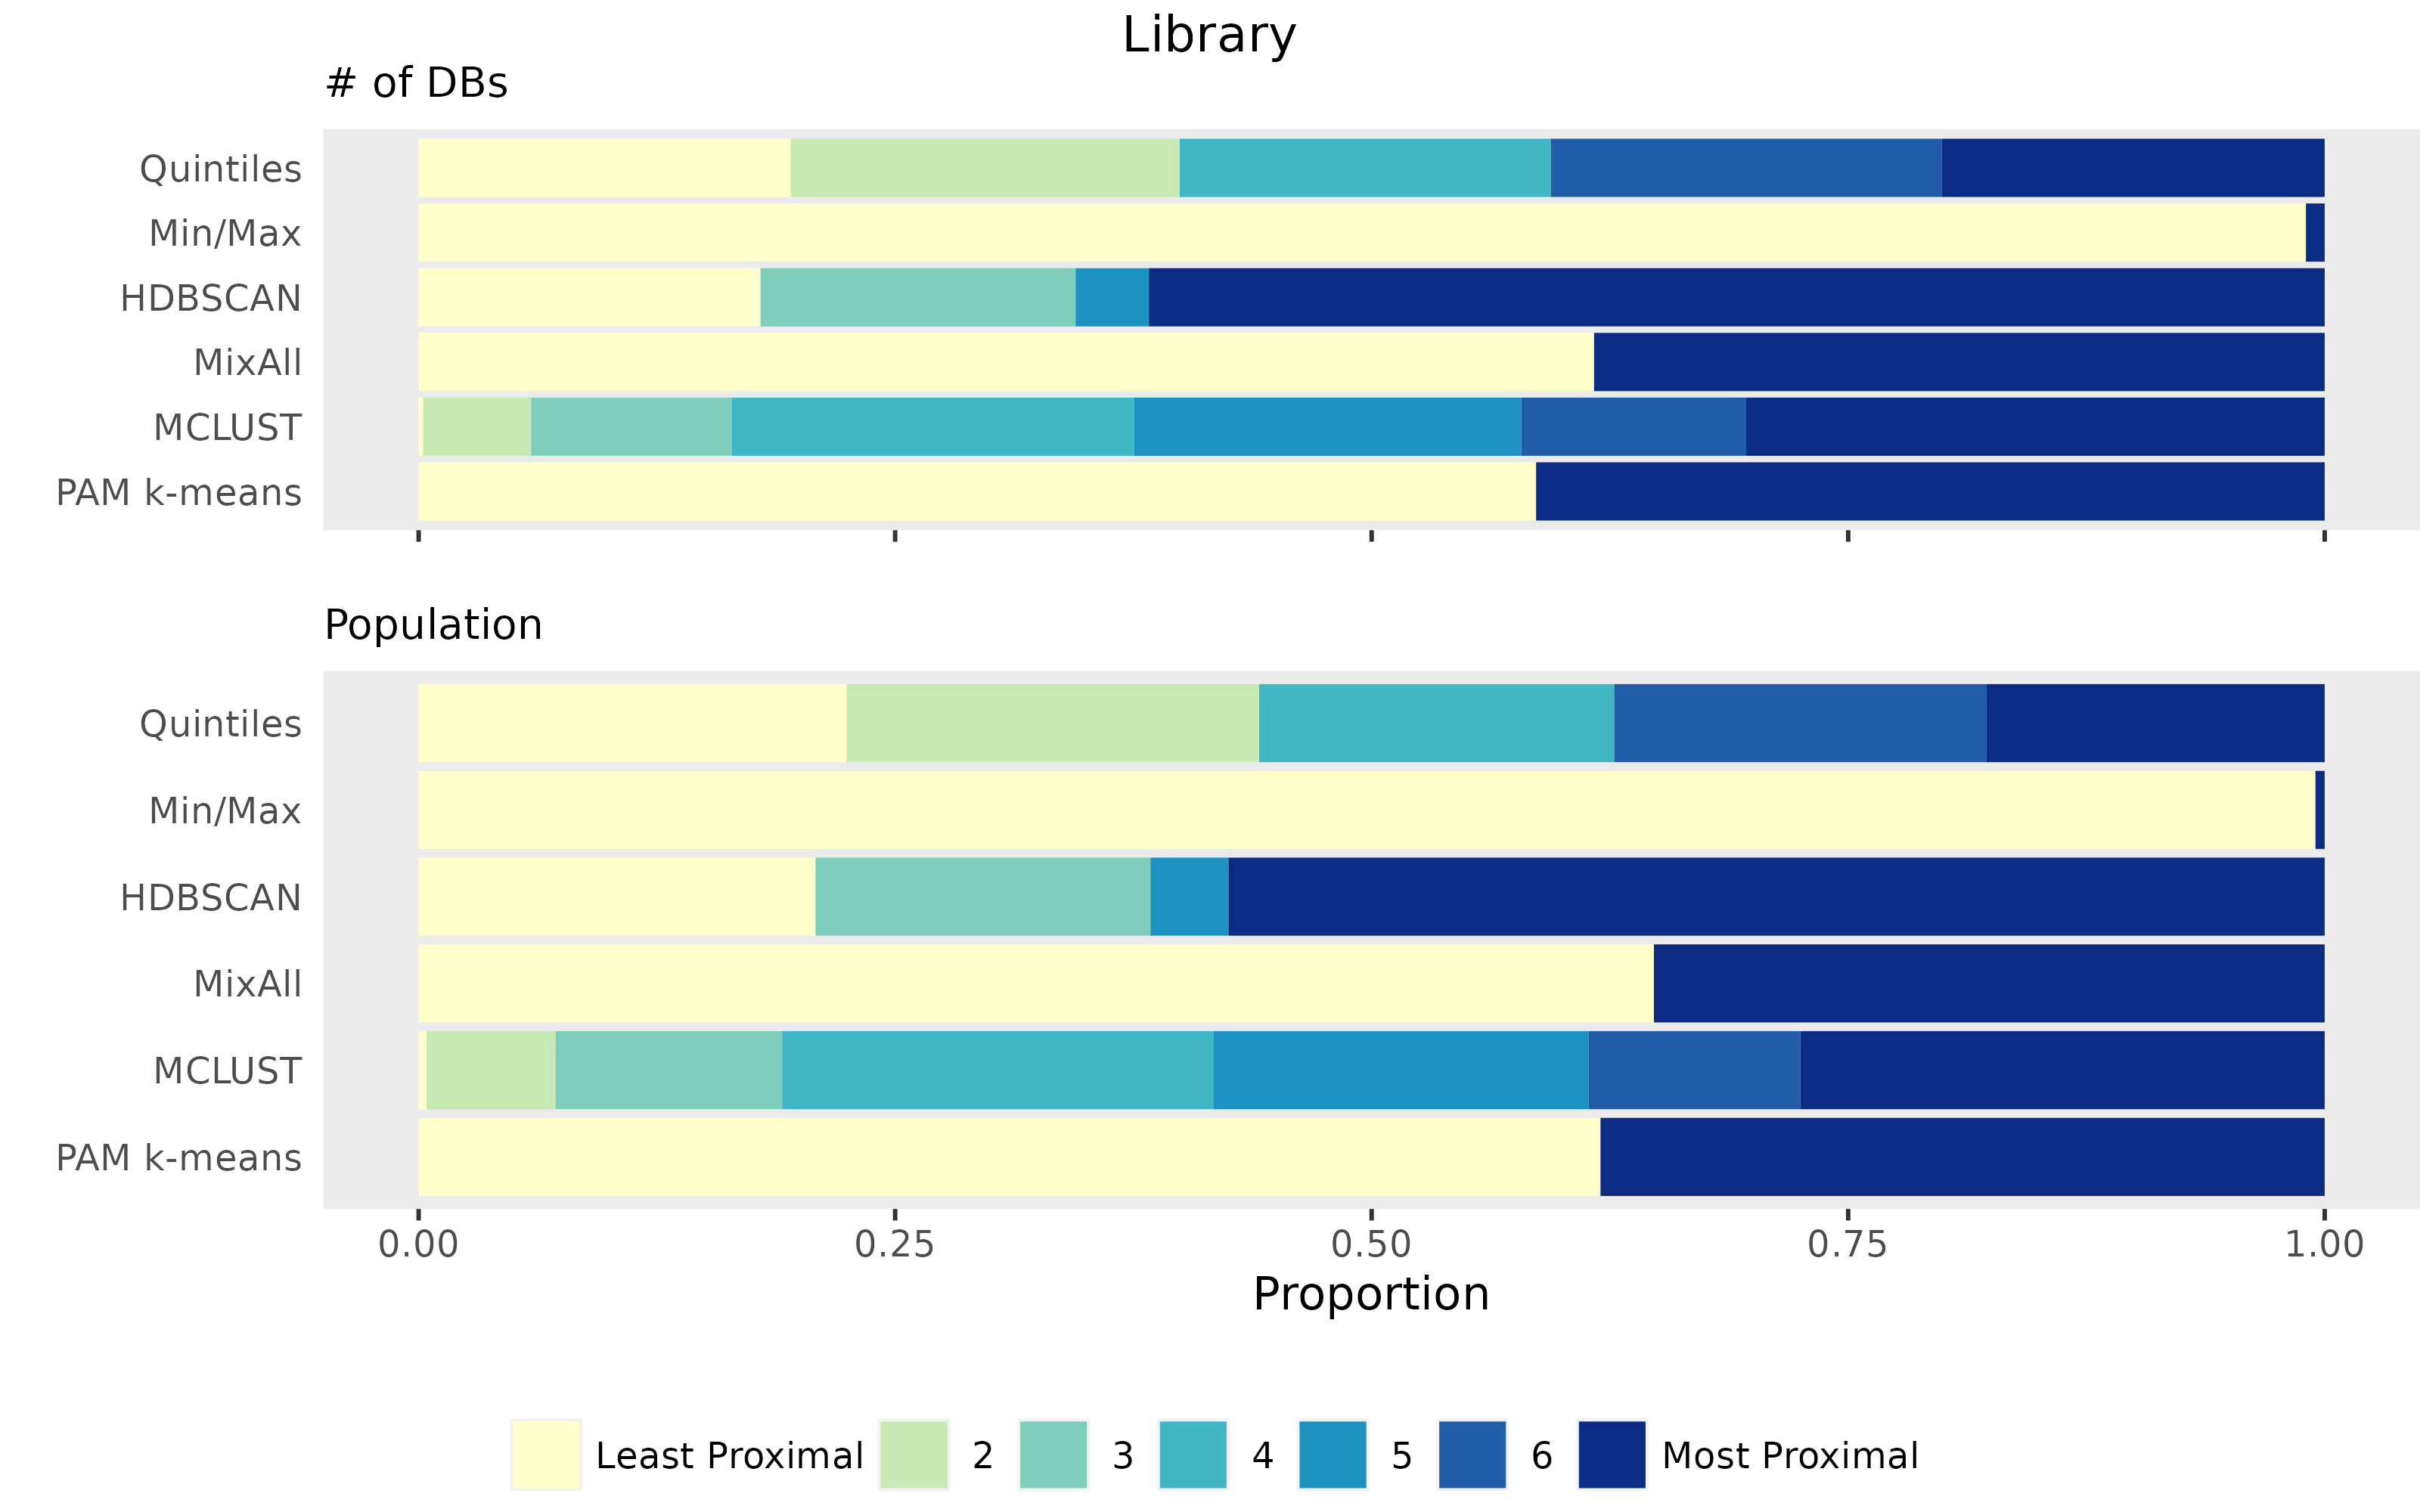
\includegraphics[width=\textwidth]{./barplot_comparison/Library_barplot.png}
\caption[Library profile barplot]{Proportion of DBs and population in each cluster for all approaches for the library amenity.}\label{librarybarplot}
\end{figure}









\begin{figure}[H]
\centering
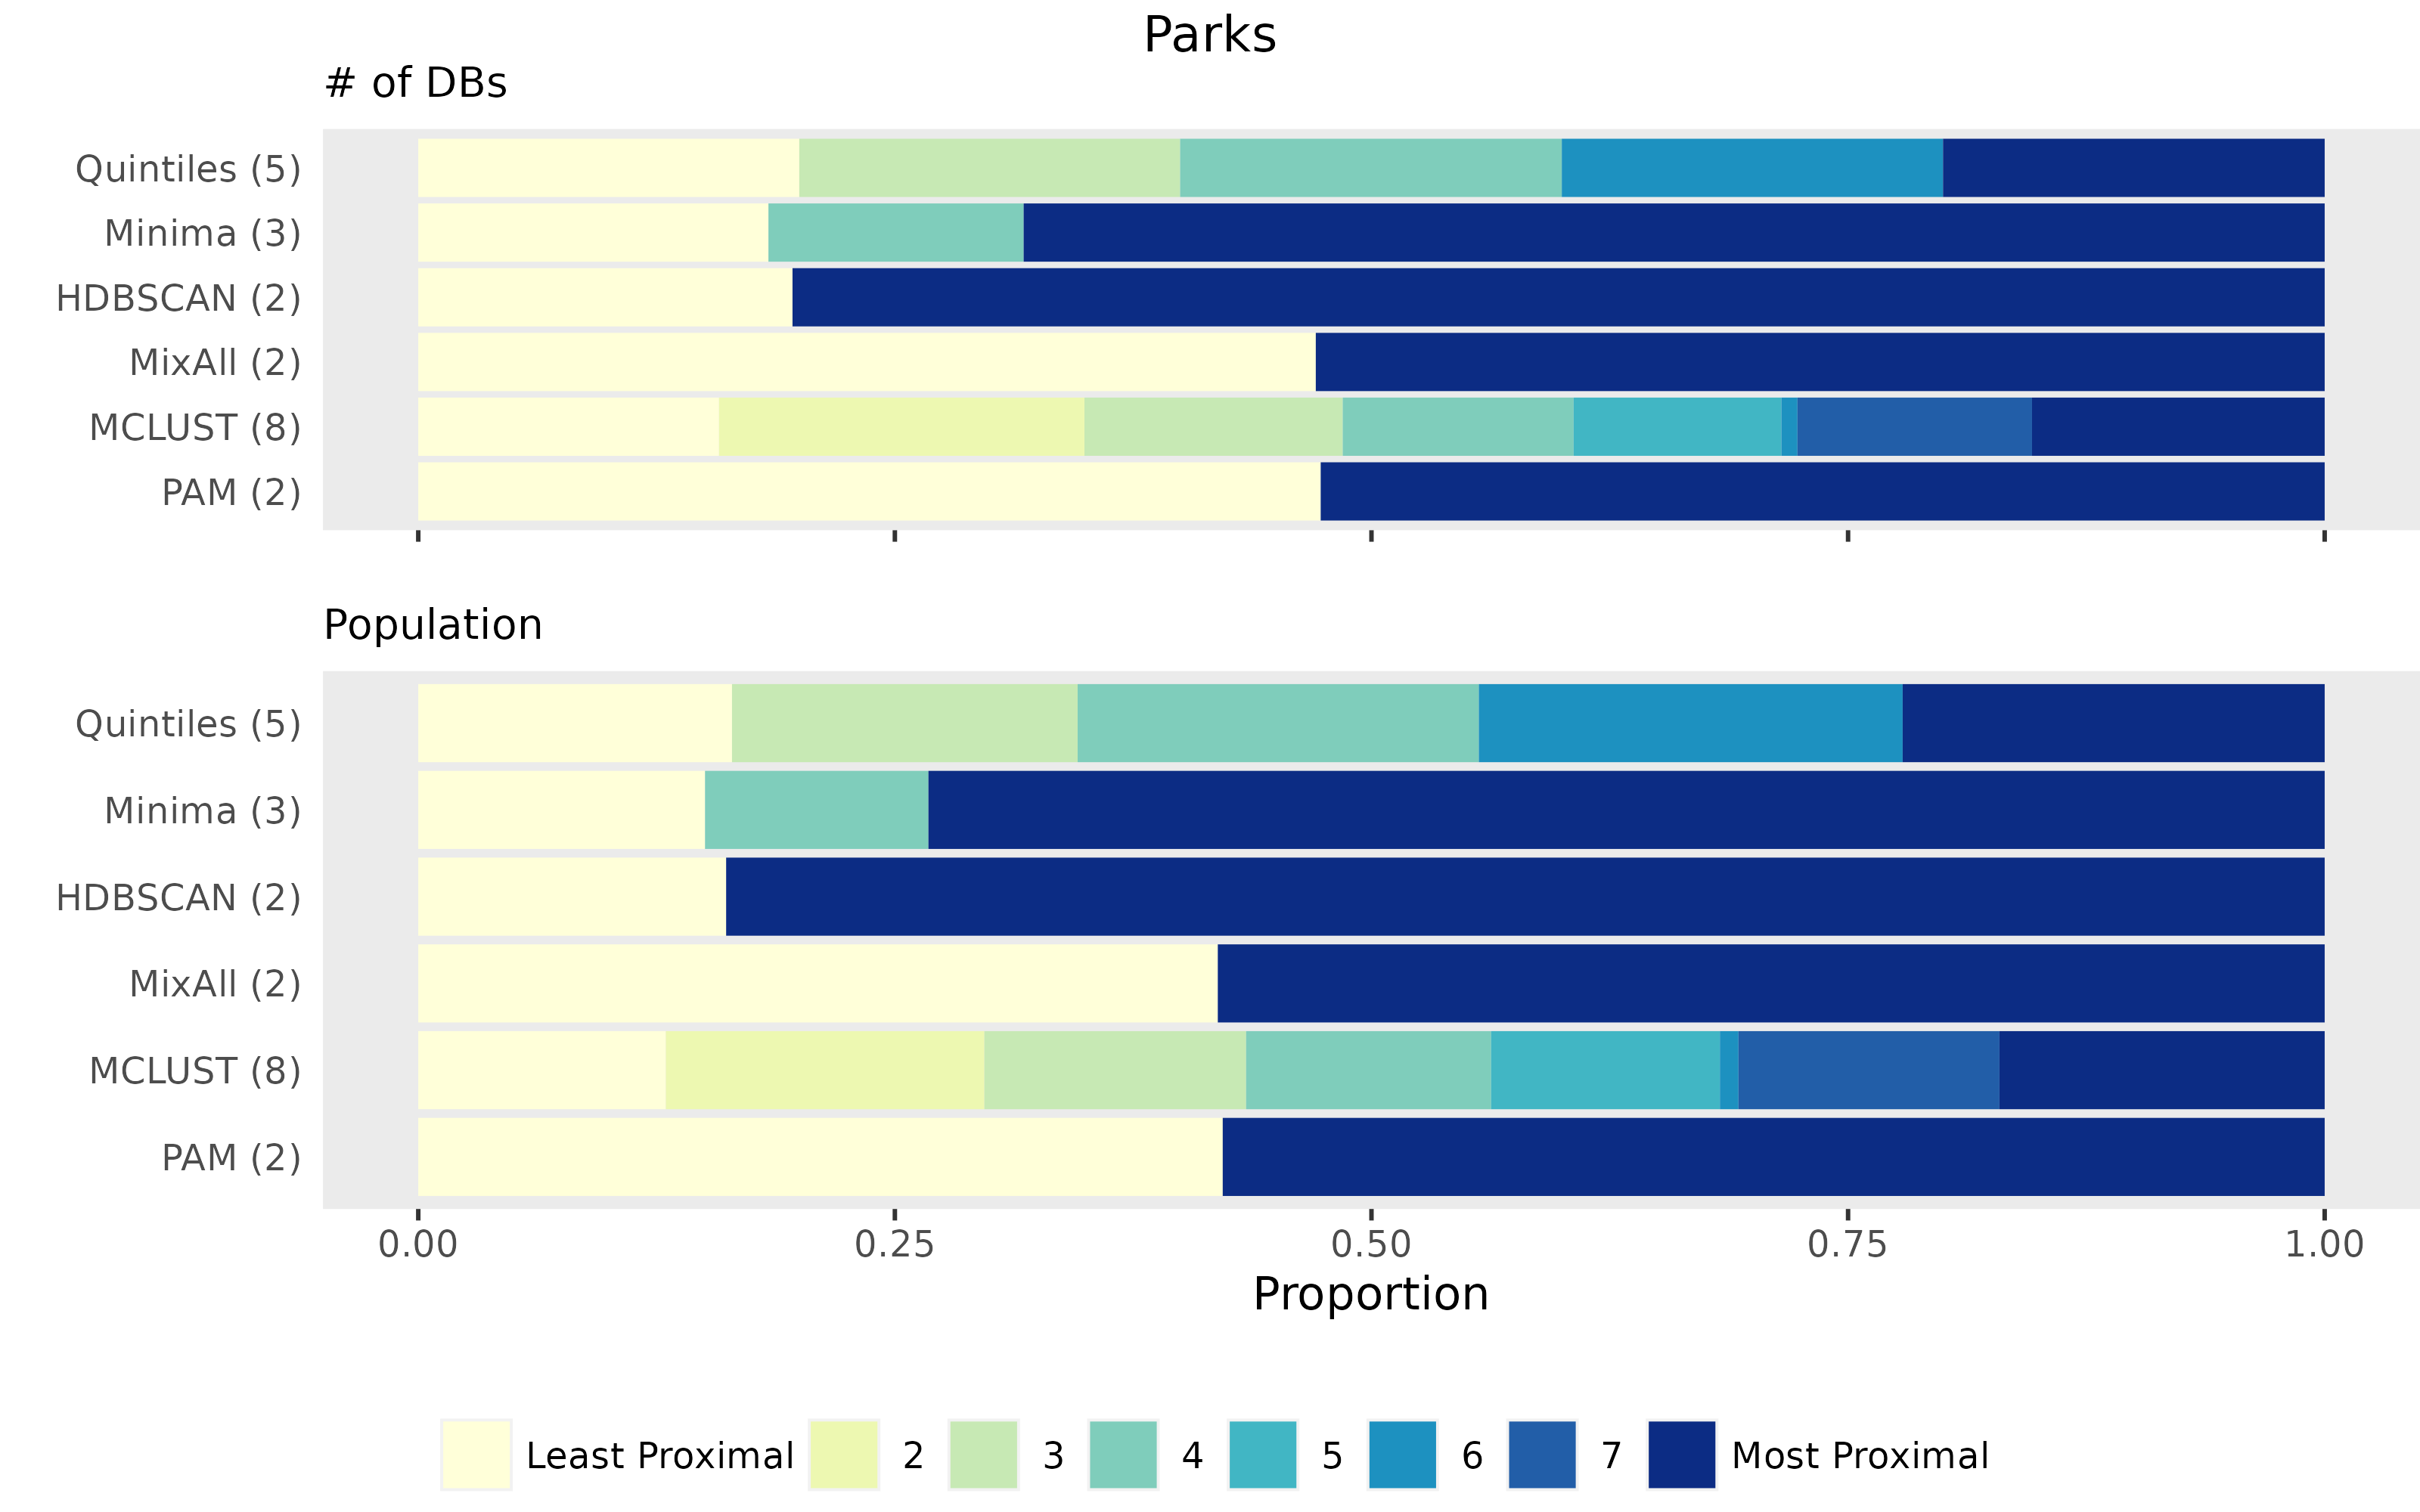
\includegraphics[width=\textwidth]{./barplot_comparison/Parks_barplot.png}
\caption[Parks profile barplot]{Proportion of DBs and population in each cluster for all approaches for the parks amenity.}\label{parksbarplot}
\end{figure}









\begin{figure}[H]
\centering
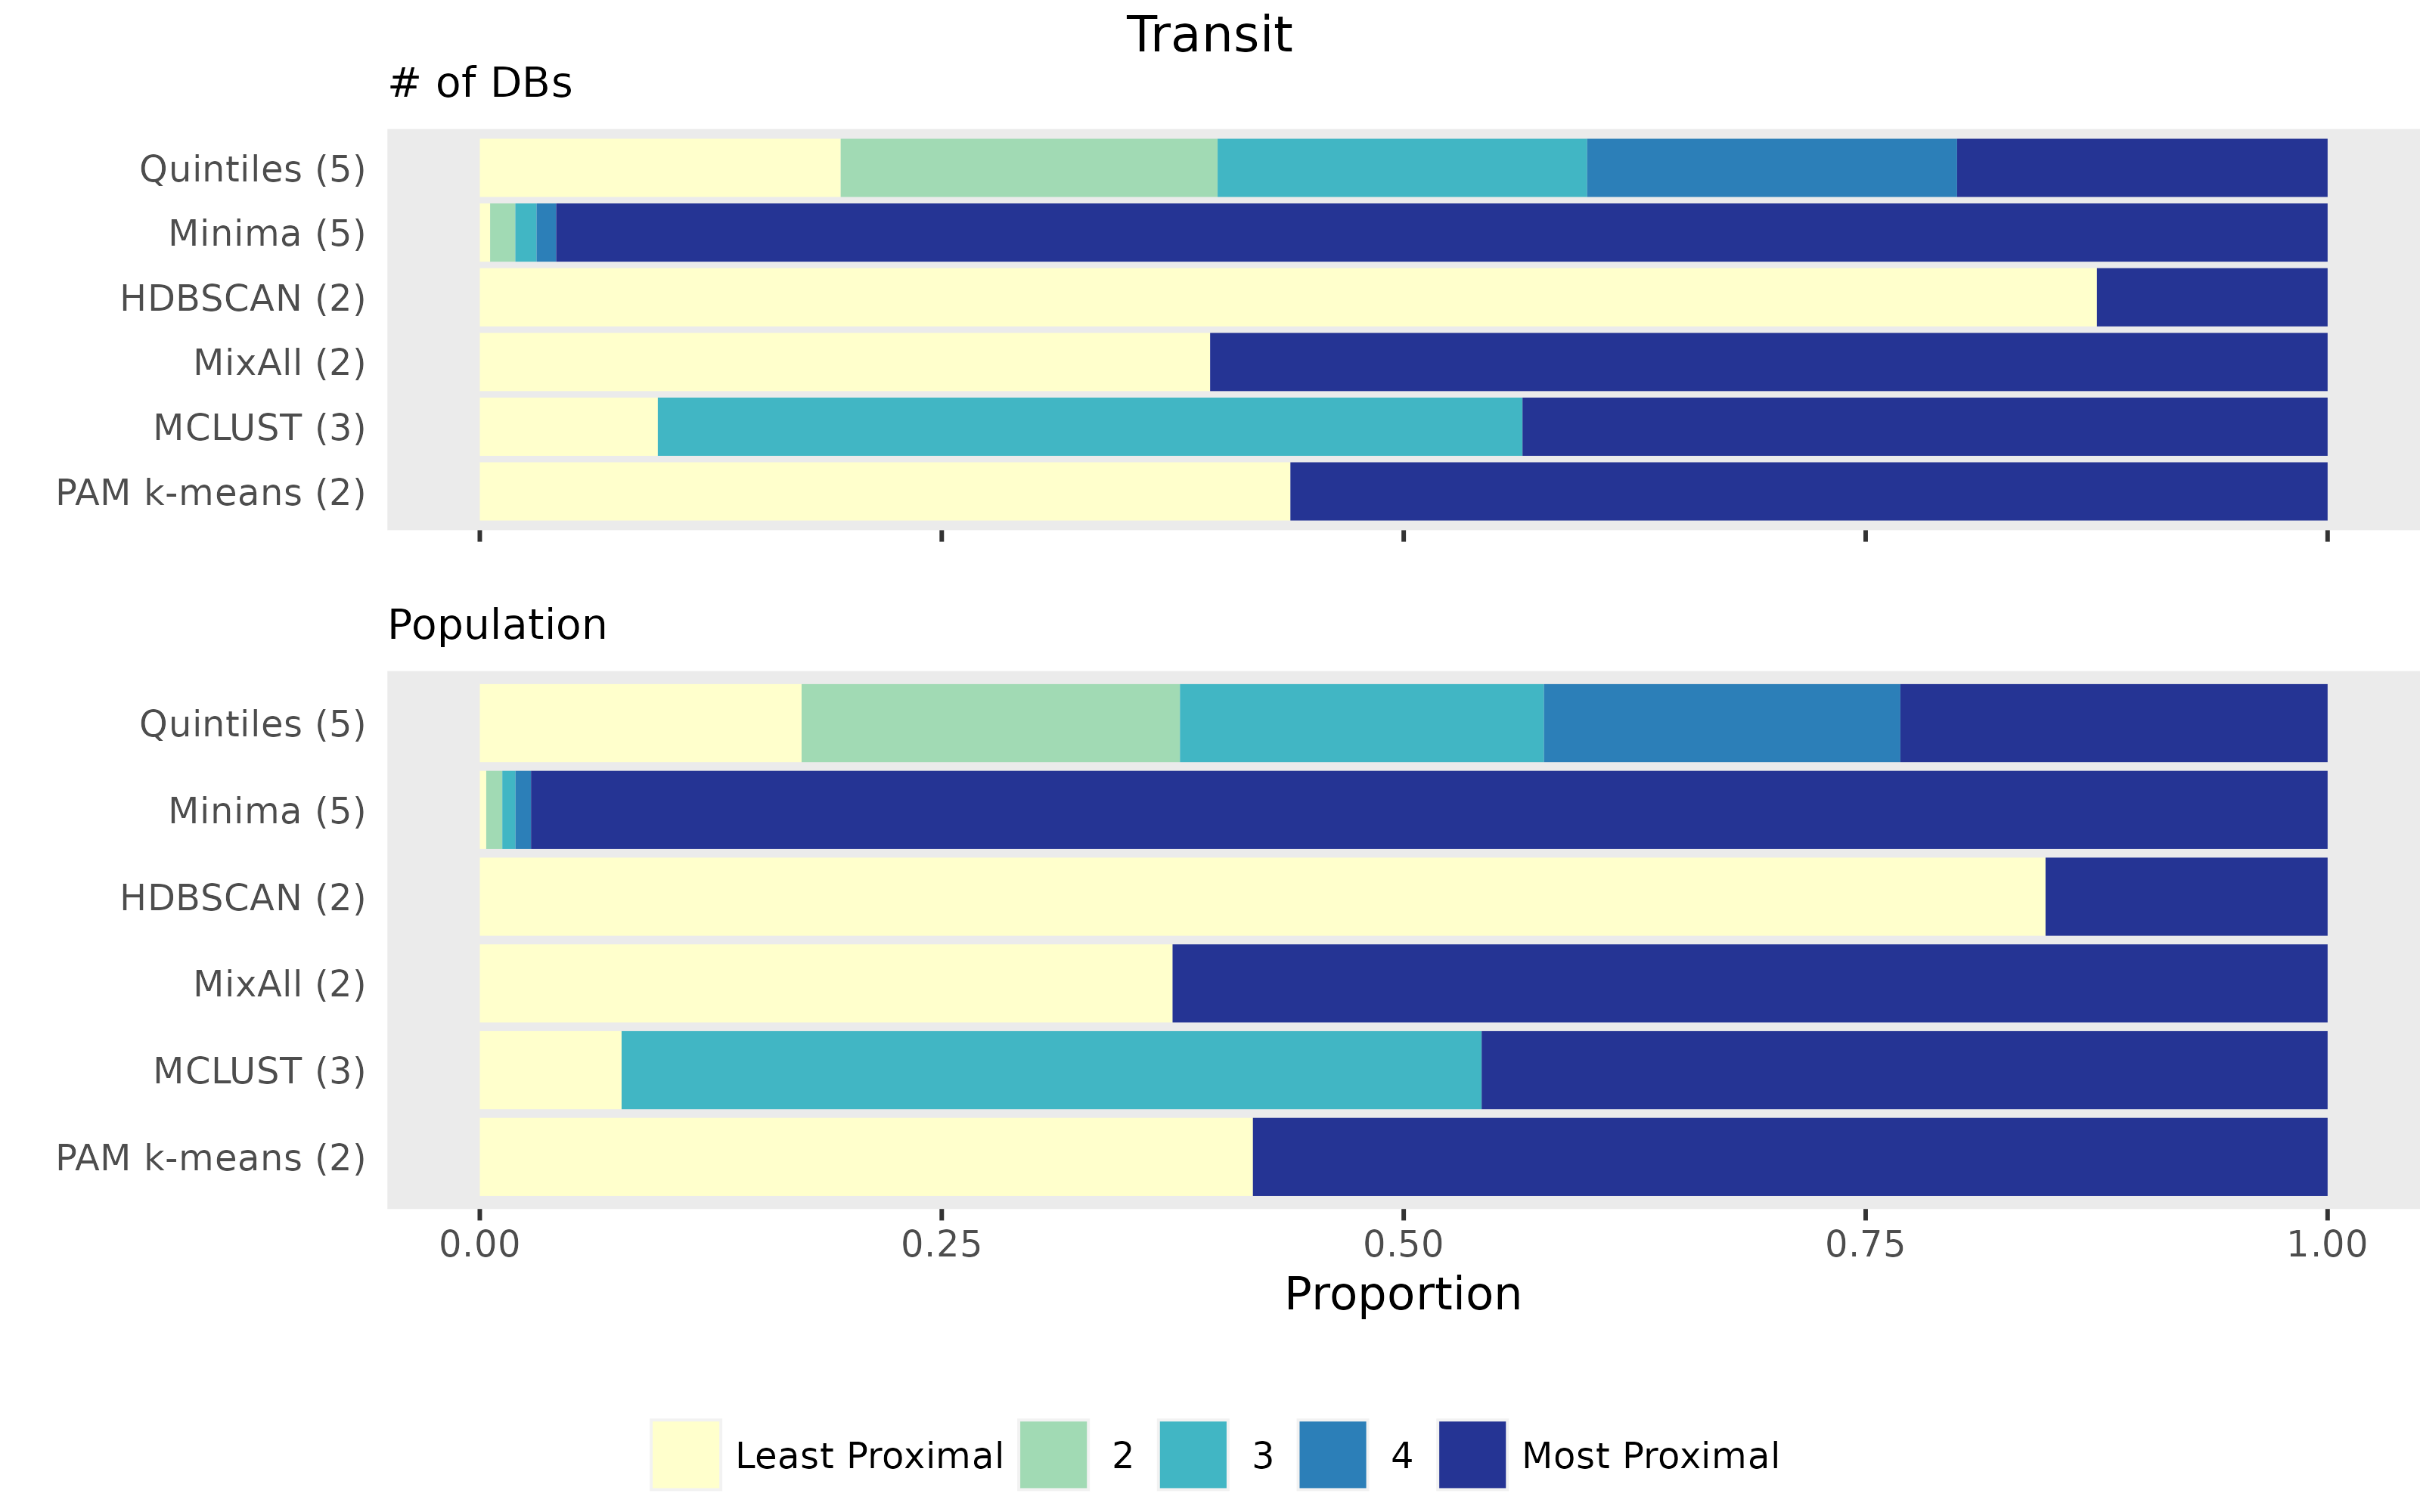
\includegraphics[width=\textwidth]{./barplot_comparison/Transit_barplot.png}
\caption[Transit profile barplot]{Proportion of DBs and population in each cluster for all approaches for the transit amenity.}\label{transitbarplot}
\end{figure}



















\begin{table}[H]
\centering
\resizebox{\textwidth}{!}{
\begin{tabular}{|r|llllllll|}
  \hline
 & \# of DBs & DB Population & Median IoR & CMA Type & Province & Amenity Dense & Employment & Range \\ 
  \hline
Entire Population & 423,602 (100.0\%) & 38 & 0.16 & CMA (48.3\%) & Ontario (18.2\%) & Low (90.1\%) & 0.006 & 0 - 1 \\ 
  Quintiles C1 & 78,014 (18.4\%) & 10 & 0.29 & None (80.9\%) & NovaScotia (6.5\%) & Low (100.0\%) & 0.000 & 0 - 4e-04 \\ 
  Min/Max C1 & 29,831 (7.0\%) & 5 & 0.32 & None (83.6\%) & NovaScotia (8.8\%) & Low (100.0\%) & 0.000 & 0 - 0.0000 \\ 
  HDBSCAN C1 & 419,062 (98.9\%) & 38 & 0.16 & CMA (47.7\%) & Ontario (17.9\%) & Low (90.9\%) & 0.006 & 0 - 0.2298 \\ 
  MixAll C1 & 179,334 (42.3\%) & 16 & 0.27 & None (73.6\%) & Ontario (7.2\%) & Low (99.9\%) & 0.000 & 0 - 0.0036 \\ 
  MCLUST C1 & 29,831 (7.0\%) & 5 & 0.32 & None (83.6\%) & NovaScotia (8.8\%) & Low (100.0\%) & 0.000 & 0 - 0.0000 \\ 
  PAM k-means C1 & 177,804 (42.0\%) & 16 & 0.27 & None (73.8\%) & Ontario (7.1\%) & Low (99.9\%) & 0.000 & 0 - 0.0035 \\ 
  Quintiles C2 & 89,705 (21.2\%) & 23 & 0.24 & None (69.6\%) & Ontario (9.2\%) & Low (99.9\%) & 0.001 & 4e-04 - 0.0030 \\ 
  Min/Max C2 & 22,179 (5.2\%) & 10 & 0.30 & None (81.2\%) & NovaScotia (5.6\%) & Low (100.0\%) & 0.000 & 0.0000 - 2e-04 \\ 
  HDBSCAN C2 & 4,540 (1.1\%) & 122 & 0.03 & CMA (100.0\%) & Ontario (44.9\%) & Med (45.9\%) & 0.292 & 0.2298 - 1 \\ 
  MixAll C2 & 244,268 (57.7\%) & 63 & 0.11 & CMA (73.3\%) & Ontario (26.3\%) & Low (82.8\%) & 0.023 & 0.0036 - 1 \\ 
  MCLUST C2 & 56,902 (13.4\%) & 10 & 0.27 & None (78.6\%) & Ontario (6.3\%) & Low (100.0\%) & 0.000 & 0.0000 - 4e-04 \\ 
  PAM k-means C2 & 245,798 (58.0\%) & 62 & 0.11 & CMA (73.0\%) & Ontario (26.2\%) & Low (82.9\%) & 0.023 & 0.0035 - 1 \\ 
  Quintiles C3 & 85,928 (20.3\%) & 41 & 0.20 & CMA (34.2\%) & Ontario (12.7\%) & Low (97.8\%) & 0.006 & 0.0030 - 0.0127 \\ 
  Min/Max C3 & 14,893 (3.5\%) & 10 & 0.27 & None (78.3\%) & Ontario (6.7\%) & Low (100.0\%) & 0.000 & 2e-04 - 3e-04 \\ 
  MCLUST C3 & 39,730 (9.4\%) & 20 & 0.24 & None (72.7\%) & Ontario (9.4\%) & Low (99.9\%) & 0.001 & 4e-04 - 0.0012 \\ 
  Quintiles C4 & 85,096 (20.1\%) & 65 & 0.11 & CMA (79.7\%) & Ontario (26.9\%) & Low (89.9\%) & 0.022 & 0.0127 - 0.0368 \\ 
  Min/Max C4 & 26,887 (6.3\%) & 17 & 0.23 & None (75.4\%) & Ontario (8.6\%) & Low (100.0\%) & 0.000 & 3e-04 - 5e-04 \\ 
  MCLUST C4 & 48,188 (11.4\%) & 27 & 0.25 & None (64.2\%) & Ontario (9.3\%) & Low (99.7\%) & 0.002 & 0.0012 - 0.0033 \\ 
  Quintiles C5 & 84,859 (20.0\%) & 83 & 0.06 & CMA (99.5\%) & Ontario (37.2\%) & Low (62.8\%) & 0.072 & 0.0368 - 1 \\ 
  Min/Max C5 & 329,812 (77.9\%) & 50 & 0.14 & CMA (59.1\%) & Ontario (21.9\%) & Low (87.2\%) & 0.014 & 5e-04 - 1 \\ 
  MCLUST C5 & 53,628 (12.7\%) & 38 & 0.21 & None (37.2\%) & Ontario (11.3\%) & Low (98.5\%) & 0.005 & 0.0033 - 0.0085 \\ 
  MCLUST C6 & 64,056 (15.1\%) & 57 & 0.14 & CMA (61.2\%) & Ontario (19.1\%) & Low (93.8\%) & 0.014 & 0.0085 - 0.0206 \\ 
  MCLUST C7 & 69,082 (16.3\%) & 71 & 0.10 & CMA (91.8\%) & Ontario (34.7\%) & Low (85.2\%) & 0.032 & 0.0206 - 0.0518 \\ 
  MCLUST C8 & 51,824 (12.2\%) & 82 & 0.06 & CMA (99.8\%) & Ontario (36.4\%) & Low (63.8\%) & 0.081 & 0.0518 - 0.1629 \\ 
  MCLUST C9 & 10,361 (2.4\%) & 118 & 0.03 & CMA (100.0\%) & Quebec (37.9\%) & Med (46.0\%) & 0.219 & 0.1629 - 1 \\ 
   \hline
\end{tabular}
}
\caption[Employment cluster profiles]{Summary statistics for each cluster found by all approaches for the employment amenity. DB Population, IoR and proximity value show the median, while CMA Type, Province and Amenity Dense show the mode.}\label{employmentprofiles}
\end{table}









\begin{table}[H]
\centering
\resizebox{\textwidth}{!}{
\begin{tabular}{|r|llllllll|}
  \hline
 & \# of DBs & DB Population & Median IoR & CMA Type & Province & Amenity Dense & Pharmacy & Range \\ 
  \hline
Entire Population & 178,521 (100.0\%) & 63 & 0.11 & CMA (71.7\%) & Ontario (27.4\%) & Low (76.4\%) & 0.026 & 0 - 1 \\ 
  Quintiles C1 & 34,980 (19.6\%) & 60 & 0.13 & CMA (64.1\%) & Ontario (21.8\%) & Low (91.5\%) & 0.007 & 0 - 0.0098 \\ 
  Min/Max C1 & 41,305 (23.1\%) & 59 & 0.13 & CMA (63.9\%) & Ontario (22.0\%) & Low (91.6\%) & 0.008 & 0 - 0.0114 \\ 
  HDBSCAN C1 & 42,510 (23.8\%) & 59 & 0.13 & CMA (63.9\%) & Ontario (22.0\%) & Low (91.6\%) & 0.008 & 0 - 0.0118 \\ 
  MixAll C1 & 91,454 (51.2\%) & 60 & 0.12 & CMA (66.7\%) & Ontario (24.1\%) & Low (88.6\%) & 0.013 & 0 - 0.0265 \\ 
  MCLUST C1 & 3,222 (1.8\%) & 70 & 0.14 & CMA (60.5\%) & Ontario (20.7\%) & Low (93.5\%) & 0.006 & 0 - 0.0064 \\ 
  PAM k-means C1 & 90,986 (51.0\%) & 60 & 0.12 & CMA (66.6\%) & Ontario (24.1\%) & Low (88.7\%) & 0.013 & 0 - 0.0263 \\ 
  Quintiles C2 & 36,365 (20.4\%) & 60 & 0.12 & CMA (66.8\%) & Ontario (24.4\%) & Low (88.7\%) & 0.014 & 0.0098 - 0.0193 \\ 
  Min/Max C2 & 30,505 (17.1\%) & 60 & 0.11 & CMA (67.7\%) & Ontario (24.7\%) & Low (87.9\%) & 0.015 & 0.0114 - 0.0195 \\ 
  HDBSCAN C2 & 90,111 (50.5\%) & 63 & 0.11 & CMA (71.5\%) & Ontario (27.9\%) & Low (81.2\%) & 0.025 & 0.0118 - 0.0525 \\ 
  MixAll C2 & 87,067 (48.8\%) & 67 & 0.10 & CMA (77.0\%) & Ontario (30.9\%) & Low (63.6\%) & 0.055 & 0.0265 - 1 \\ 
  MCLUST C2 & 35,979 (20.2\%) & 59 & 0.13 & CMA (64.3\%) & Ontario (22.0\%) & Low (91.4\%) & 0.008 & 0.0064 - 0.0108 \\ 
  PAM k-means C2 & 87,535 (49.0\%) & 67 & 0.10 & CMA (77.0\%) & Ontario (30.9\%) & Low (63.7\%) & 0.055 & 0.0263 - 1 \\ 
  Quintiles C3 & 35,730 (20.0\%) & 63 & 0.11 & CMA (72.1\%) & Ontario (28.5\%) & Low (81.3\%) & 0.026 & 0.0193 - 0.0341 \\ 
  Min/Max C3 & 106,711 (59.8\%) & 66 & 0.11 & CMA (75.8\%) & Ontario (30.3\%) & Low (67.2\%) & 0.046 & 0.0195 - 1 \\ 
  HDBSCAN C3 & 45,900 (25.7\%) & 70 & 0.09 & CMA (79.2\%) & Ontario (31.5\%) & Low (52.9\%) & 0.085 & 0.0525 - 1 \\ 
  MCLUST C3 & 2,075 (1.2\%) & 56 & 0.13 & CMA (61.8\%) & Ontario (23.1\%) & Low (92.8\%) & 0.011 & 0.0108 - 0.0114 \\ 
  Quintiles C4 & 35,697 (20.0\%) & 66 & 0.11 & CMA (75.0\%) & Ontario (30.9\%) & Low (72.0\%) & 0.046 & 0.0341 - 0.0641 \\ 
  MCLUST C4 & 26,864 (15.0\%) & 60 & 0.11 & CMA (67.5\%) & Ontario (24.7\%) & Low (88.1\%) & 0.015 & 0.0114 - 0.0181 \\ 
  Quintiles C5 & 35,749 (20.0\%) & 71 & 0.08 & CMA (80.3\%) & Ontario (31.6\%) & Low (48.5\%) & 0.098 & 0.0641 - 1 \\ 
  MCLUST C5 & 37,376 (20.9\%) & 62 & 0.11 & CMA (71.8\%) & Ontario (28.1\%) & Low (82.0\%) & 0.025 & 0.0181 - 0.0332 \\ 
  MCLUST C6 & 30,077 (16.8\%) & 65 & 0.11 & CMA (74.9\%) & Ontario (30.8\%) & Low (73.1\%) & 0.042 & 0.0332 - 0.0554 \\ 
  MCLUST C7 & 42,928 (24.0\%) & 70 & 0.09 & CMA (79.5\%) & Ontario (31.5\%) & Low (51.8\%) & 0.088 & 0.0554 - 1 \\ 
   \hline
\end{tabular}
}
\caption[Pharmacy cluster profiles]{Summary statistics for each cluster found by all approaches for the pharmacy amenity. DB Population, IoR and proximity value show the median, while CMA Type, Province and Amenity Dense show the mode.}\label{pharmacyprofiles}
\end{table}










\begin{table}[H]
\centering
\resizebox{\textwidth}{!}{
\begin{tabular}{|r|llllllll|}
  \hline
 & \# of DBs & DB Population & Median IoR & CMA Type & Province & Amenity Dense & Childcare & Range \\ 
  \hline
Entire Population & 243,964 (100.0\%) & 62 & 0.11 & CMA (68.3\%) & Ontario (23.9\%) & Low (82.7\%) & 0.048 & 0 - 1 \\ 
  Quintiles C1 & 48,703 (20.0\%) & 41 & 0.18 & CMA (46.5\%) & Ontario (20.9\%) & Low (96.2\%) & 0.008 & 0 - 0.0152 \\ 
  Min/Max C1 & 26,274 (10.8\%) & 40 & 0.19 & CMA (43.6\%) & Ontario (18.9\%) & Low (96.9\%) & 0.006 & 0 - 0.0084 \\ 
  HDBSCAN C1 & 27,765 (11.4\%) & 40 & 0.19 & CMA (43.5\%) & Ontario (18.9\%) & Low (96.9\%) & 0.006 & 0 - 0.0090 \\ 
  MixAll C1 & 100,768 (41.3\%) & 49 & 0.15 & CMA (54.1\%) & Ontario (25.3\%) & Low (93.5\%) & 0.016 & 0 - 0.0363 \\ 
  MCLUST C1 & 172 (0.1\%) & 231 & 0.29 & None (66.9\%) & Quebec (8.7\%) & Low (100.0\%) & 0.001 & 0 - 0.0019 \\ 
  PAM k-means C1 & 100,954 (41.4\%) & 49 & 0.15 & CMA (54.1\%) & Ontario (25.3\%) & Low (93.5\%) & 0.016 & 0 - 0.0364 \\ 
  Quintiles C2 & 48,757 (20.0\%) & 55 & 0.13 & CMA (60.8\%) & Ontario (29.4\%) & Low (91.3\%) & 0.024 & 0.0152 - 0.0348 \\ 
  Min/Max C2 & 18,663 (7.6\%) & 43 & 0.16 & CMA (49.7\%) & Ontario (23.2\%) & Low (95.4\%) & 0.011 & 0.0084 - 0.0139 \\ 
  HDBSCAN C2 & 216,199 (88.6\%) & 65 & 0.11 & CMA (71.5\%) & Ontario (24.5\%) & Low (80.9\%) & 0.056 & 0.0090 - 1 \\ 
  MixAll C2 & 143,196 (58.7\%) & 71 & 0.11 & CMA (78.3\%) & Ontario (22.9\%) & Low (75.2\%) & 0.086 & 0.0363 - 1 \\ 
  MCLUST C2 & 150,501 (61.7\%) & 55 & 0.14 & CMA (60.1\%) & Ontario (26.2\%) & Low (90.3\%) & 0.025 & 0.0019 - 0.0669 \\ 
  PAM k-means C2 & 143,010 (58.6\%) & 71 & 0.11 & CMA (78.3\%) & Ontario (22.8\%) & Low (75.1\%) & 0.086 & 0.0364 - 1 \\ 
  Quintiles C3 & 48,909 (20.0\%) & 66 & 0.11 & CMA (71.5\%) & Ontario (28.3\%) & Low (84.4\%) & 0.048 & 0.0348 - 0.0636 \\ 
  Min/Max C3 & 199,027 (81.6\%) & 67 & 0.11 & CMA (73.3\%) & Ontario (24.6\%) & Low (79.7\%) & 0.062 & 0.0139 - 1 \\ 
  MCLUST C3 & 93,291 (38.2\%) & 74 & 0.10 & CMA (81.6\%) & Quebec (22.7\%) & Low (70.5\%) & 0.120 & 0.0669 - 1 \\ 
  Quintiles C4 & 48,776 (20.0\%) & 69 & 0.11 & CMA (77.0\%) & Ontario (23.8\%) & Low (78.4\%) & 0.085 & 0.0636 - 0.1167 \\ 
  Quintiles C5 & 48,819 (20.0\%) & 80 & 0.08 & CMA (85.7\%) & Quebec (35.3\%) & Low (63.4\%) & 0.175 & 0.1167 - 1 \\ 
   \hline
\end{tabular}
}
\caption[Child care cluster profiles]{Summary statistics for each cluster found by all approaches for the child care amenity. DB Population, IoR and proximity value show the median, while CMA Type, Province and Amenity Dense show the mode.}\label{childcareprofiles}
\end{table}










\begin{table}[H]
\centering
\resizebox{\textwidth}{!}{
\begin{tabular}{|r|llllllll|}
  \hline
 & \# of DBs & DB Population & Median IoR & CMA Type & Province & Amenity Dense & Healthcare & Range \\ 
  \hline
Entire Population & 300,465 (100.0\%) & 55 & 0.13 & CMA (62.2\%) & Ontario (22.8\%) & Low (86.0\%) & 0.005 & 0 - 1 \\ 
  Quintiles C1 & 56,525 (18.8\%) & 26 & 0.20 & None (48.0\%) & Ontario (12.1\%) & Low (99.7\%) & 0.000 & 0 - 7e-04 \\ 
  Min/Max C1 & 14,556 (4.8\%) & 23 & 0.19 & None (56.5\%) & Ontario (14.7\%) & Low (99.8\%) & 0.000 & 0 - 0.0000 \\ 
  HDBSCAN C1 & 295,804 (98.4\%) & 54 & 0.13 & CMA (61.7\%) & Ontario (22.6\%) & Low (87.0\%) & 0.005 & 0 - 0.1052 \\ 
  MixAll C1 & 106,196 (35.3\%) & 35 & 0.19 & None (40.2\%) & Ontario (13.2\%) & Low (98.7\%) & 0.001 & 0 - 0.0025 \\ 
  MCLUST C1 & 36,901 (12.3\%) & 25 & 0.20 & None (50.8\%) & Ontario (13.2\%) & Low (99.7\%) & 0.000 & 0 - 2e-04 \\ 
  PAM k-means C1 & 99,871 (33.2\%) & 34 & 0.19 & None (41.2\%) & Ontario (12.9\%) & Low (98.9\%) & 0.000 & 0 - 0.0022 \\ 
  Quintiles C2 & 61,910 (20.6\%) & 48 & 0.15 & CMA (50.9\%) & Ontario (15.4\%) & Low (97.1\%) & 0.002 & 7e-04 - 0.0032 \\ 
  Min/Max C2 & 14,259 (4.7\%) & 26 & 0.20 & None (48.7\%) & Ontario (12.6\%) & Low (99.8\%) & 0.000 & 0.0000 - 2e-04 \\ 
  HDBSCAN C2 & 4,661 (1.6\%) & 102 & 0.03 & CMA (95.4\%) & Ontario (38.3\%) & Med (43.5\%) & 0.142 & 0.1052 - 1 \\ 
  MixAll C2 & 194,269 (64.7\%) & 67 & 0.11 & CMA (74.4\%) & Ontario (28.1\%) & Low (79.0\%) & 0.010 & 0.0025 - 1 \\ 
  MCLUST C2 & 87,182 (29.0\%) & 44 & 0.16 & CMA (48.3\%) & Ontario (14.6\%) & Low (97.4\%) & 0.001 & 2e-04 - 0.0034 \\ 
  PAM k-means C2 & 200,594 (66.8\%) & 66 & 0.11 & CMA (73.8\%) & Ontario (27.8\%) & Low (79.6\%) & 0.010 & 0.0022 - 1 \\ 
  Quintiles C3 & 61,500 (20.5\%) & 66 & 0.11 & CMA (69.5\%) & Ontario (25.6\%) & Low (91.7\%) & 0.005 & 0.0032 - 0.0074 \\ 
  Min/Max C3 & 8,086 (2.7\%) & 26 & 0.20 & None (44.4\%) & Ontario (11.4\%) & Low (99.6\%) & 0.000 & 2e-04 - 3e-04 \\ 
  MCLUST C3 & 74,409 (24.8\%) & 67 & 0.11 & CMA (70.5\%) & Ontario (26.7\%) & Low (90.2\%) & 0.006 & 0.0034 - 0.0093 \\ 
  Quintiles C4 & 60,378 (20.1\%) & 65 & 0.11 & CMA (71.4\%) & Ontario (28.7\%) & Low (83.4\%) & 0.011 & 0.0074 - 0.0184 \\ 
  Min/Max C4 & 263,564 (87.7\%) & 60 & 0.12 & CMA (66.6\%) & Ontario (24.2\%) & Low (84.1\%) & 0.006 & 3e-04 - 1 \\ 
  MCLUST C4 & 101,973 (33.9\%) & 68 & 0.10 & CMA (79.4\%) & Ontario (30.5\%) & Low (68.1\%) & 0.022 & 0.0093 - 1 \\ 
  Quintiles C5 & 60,152 (20.0\%) & 71 & 0.10 & CMA (85.2\%) & Ontario (31.7\%) & Low (58.5\%) & 0.034 & 0.0184 - 1 \\ 
   \hline
\end{tabular}
}
\caption[Health care cluster profiles]{Summary statistics for each cluster found by all approaches for the health care amenity. DB Population, IoR and proximity value show the median, while CMA Type, Province and Amenity Dense show the mode.}\label{healthcareprofiles}
\end{table}










\begin{table}[H]
\centering
\resizebox{\textwidth}{!}{
\begin{tabular}{|r|llllllll|}
  \hline
 & \# of DBs & DB Population & Median IoR & CMA Type & Province & Amenity Dense & Grocery & Range \\ 
  \hline
Entire Population & 141,063 (100.0\%) & 61 & 0.11 & CMA (69.3\%) & Ontario (25.1\%) & Low (70.1\%) & 0.043 & 0 - 1 \\ 
  Quintiles C1 & 27,762 (19.7\%) & 65 & 0.11 & CMA (71.9\%) & Ontario (28.1\%) & Low (81.9\%) & 0.014 & 0 - 0.0221 \\ 
  Min/Max C1 & 11,600 (8.2\%) & 67 & 0.11 & CMA (73.5\%) & Ontario (28.6\%) & Low (82.5\%) & 0.009 & 0 - 0.0121 \\ 
  HDBSCAN C1 & 11,799 (8.4\%) & 67 & 0.11 & CMA (73.4\%) & Ontario (28.5\%) & Low (82.6\%) & 0.009 & 0 - 0.0124 \\ 
  MixAll C1 & 77,110 (54.7\%) & 60 & 0.12 & CMA (66.0\%) & Ontario (25.4\%) & Low (79.9\%) & 0.027 & 0 - 0.0484 \\ 
  MCLUST C1 & 1,615 (1.1\%) & 77 & 0.11 & CMA (66.8\%) & Ontario (27.1\%) & Low (85.8\%) & 0.007 & 0 - 0.0072 \\ 
  PAM k-means C1 & 10,674 (7.6\%) & 68 & 0.11 & CMA (73.8\%) & Ontario (28.6\%) & Low (82.6\%) & 0.008 & 0 - 0.0113 \\ 
  Quintiles C2 & 28,569 (20.3\%) & 56 & 0.13 & CMA (61.3\%) & Ontario (23.2\%) & Low (80.6\%) & 0.029 & 0.0221 - 0.0348 \\ 
  Min/Max C2 & 10,766 (7.6\%) & 66 & 0.11 & CMA (72.7\%) & Ontario (28.9\%) & Low (81.6\%) & 0.016 & 0.0121 - 0.0185 \\ 
  HDBSCAN C2 & 89,898 (63.7\%) & 58 & 0.12 & CMA (65.2\%) & Ontario (25.0\%) & Low (76.8\%) & 0.035 & 0.0124 - 0.0763 \\ 
  MixAll C2 & 63,953 (45.3\%) & 64 & 0.11 & CMA (73.3\%) & Ontario (24.8\%) & Low (58.4\%) & 0.090 & 0.0484 - 1 \\ 
  MCLUST C2 & 9,542 (6.8\%) & 66 & 0.11 & CMA (74.8\%) & Ontario (28.9\%) & Low (81.9\%) & 0.009 & 0.0072 - 0.0117 \\ 
  PAM k-means C2 & 12,384 (8.8\%) & 66 & 0.11 & CMA (72.6\%) & Ontario (28.8\%) & Low (81.5\%) & 0.016 & 0.0113 - 0.0189 \\ 
  Quintiles C3 & 28,266 (20.0\%) & 58 & 0.12 & CMA (64.6\%) & Ontario (25.1\%) & Low (74.7\%) & 0.043 & 0.0348 - 0.0555 \\ 
  Min/Max C3 & 118,697 (84.1\%) & 60 & 0.11 & CMA (68.6\%) & Ontario (24.5\%) & Low (67.9\%) & 0.053 & 0.0185 - 1 \\ 
  HDBSCAN C3 & 39,366 (27.9\%) & 69 & 0.10 & CMA (77.4\%) & Ontario (24.5\%) & Low (51.2\%) & 0.126 & 0.0763 - 1 \\ 
  MCLUST C3 & 129,906 (92.1\%) & 61 & 0.11 & CMA (68.9\%) & Ontario (24.9\%) & Low (69.1\%) & 0.048 & 0.0117 - 1 \\ 
  PAM k-means C3 & 15,758 (11.2\%) & 55 & 0.14 & CMA (60.9\%) & Ontario (23.2\%) & Low (81.8\%) & 0.023 & 0.0189 - 0.0275 \\ 
  Quintiles C4 & 28,248 (20.0\%) & 58 & 0.11 & CMA (68.5\%) & Ontario (24.9\%) & Low (67.3\%) & 0.072 & 0.0555 - 0.0985 \\ 
  PAM k-means C4 & 25,218 (17.9\%) & 57 & 0.13 & CMA (63.1\%) & Ontario (24.0\%) & Low (79.0\%) & 0.033 & 0.0275 - 0.0389 \\ 
  Quintiles C5 & 28,218 (20.0\%) & 74 & 0.08 & CMA (80.3\%) & Ontario (24.5\%) & Low (46.2\%) & 0.154 & 0.0985 - 1 \\ 
  PAM k-means C5 & 22,468 (15.9\%) & 58 & 0.12 & CMA (65.2\%) & Ontario (25.2\%) & Low (73.4\%) & 0.047 & 0.0389 - 0.0574 \\ 
  PAM k-means C6 & 23,558 (16.7\%) & 58 & 0.11 & CMA (68.2\%) & Ontario (24.8\%) & Low (67.8\%) & 0.071 & 0.0574 - 0.0919 \\ 
  PAM k-means C7 & 18,749 (13.3\%) & 67 & 0.10 & CMA (75.1\%) & Ontario (25.7\%) & Low (56.1\%) & 0.119 & 0.0919 - 0.1674 \\ 
  PAM k-means C8 & 12,254 (8.7\%) & 85 & 0.06 & CMA (86.1\%) & Quebec (31.8\%) & Med (40.8\%) & 0.232 & 0.1674 - 1 \\ 
   \hline
\end{tabular}
}
\caption[Grocery cluster profiles]{Summary statistics for each cluster found by all approaches for the grocery amenity. DB Population, IoR and proximity value show the median, while CMA Type, Province and Amenity Dense show the mode.}\label{groceryprofiles}
\end{table}










\begin{table}[H]
\centering
\resizebox{\textwidth}{!}{
\begin{tabular}{|r|llllllll|}
  \hline
 & \# of DBs & DB Population & Median IoR & CMA Type & Province & Amenity Dense & Sec. Educ. & Range \\ 
  \hline
Entire Population & 141,213 (100.0\%) & 58 & 0.14 & CMA (62.5\%) & Ontario (18.2\%) & Low (77.2\%) & 0.074 & 0 - 1 \\ 
  Quintiles C1 & 28,202 (20.0\%) & 58 & 0.13 & CMA (63.4\%) & Ontario (25.6\%) & Low (82.8\%) & 0.037 & 0 - 0.0421 \\ 
  Min/Max C1 & 63,449 (44.9\%) & 56 & 0.14 & CMA (61.0\%) & Ontario (24.2\%) & Low (82.9\%) & 0.043 & 0 - 0.0661 \\ 
  HDBSCAN C1 & 55,741 (39.5\%) & 57 & 0.13 & CMA (61.8\%) & Ontario (24.6\%) & Low (82.8\%) & 0.042 & 0 - 0.0576 \\ 
  MixAll C1 & 61,440 (43.5\%) & 56 & 0.13 & CMA (61.2\%) & Ontario (24.3\%) & Low (82.9\%) & 0.043 & 0 - 0.0632 \\ 
  MCLUST C1 & 3,273 (2.3\%) & 62 & 0.14 & CMA (61.3\%) & Ontario (24.4\%) & Low (84.8\%) & 0.034 & 0 - 0.0346 \\ 
  PAM k-means C1 & 53,475 (37.9\%) & 57 & 0.13 & CMA (62.0\%) & Ontario (24.8\%) & Low (82.7\%) & 0.041 & 0 - 0.0557 \\ 
  Quintiles C2 & 28,226 (20.0\%) & 55 & 0.14 & CMA (60.1\%) & Ontario (23.5\%) & Low (82.7\%) & 0.048 & 0.0421 - 0.0586 \\ 
  Min/Max C2 & 77,764 (55.1\%) & 60 & 0.14 & CMA (63.7\%) & BritishColumbia (15.5\%) & Low (72.6\%) & 0.122 & 0.0661 - 1 \\ 
  HDBSCAN C2 & 25,135 (17.8\%) & 53 & 0.15 & CMA (58.0\%) & Ontario (19.1\%) & Low (81.3\%) & 0.072 & 0.0576 - 0.0863 \\ 
  MixAll C2 & 48,748 (34.5\%) & 56 & 0.14 & CMA (60.8\%) & Ontario (16.2\%) & Low (77.0\%) & 0.092 & 0.0632 - 0.1409 \\ 
  MCLUST C2 & 996 (0.7\%) & 62 & 0.12 & CMA (65.4\%) & Ontario (28.7\%) & Low (80.9\%) & 0.035 & 0.0346 - 0.0347 \\ 
  PAM k-means C2 & 37,062 (26.2\%) & 54 & 0.15 & CMA (58.7\%) & Ontario (18.5\%) & Low (80.3\%) & 0.076 & 0.0557 - 0.0990 \\ 
  Quintiles C3 & 28,260 (20.0\%) & 53 & 0.15 & CMA (58.4\%) & Ontario (18.6\%) & Low (80.7\%) & 0.074 & 0.0586 - 0.0910 \\ 
  HDBSCAN C3 & 60,337 (42.7\%) & 62 & 0.14 & CMA (64.9\%) & BritishColumbia (17.8\%) & Low (70.4\%) & 0.143 & 0.0863 - 1 \\ 
  MixAll C3 & 31,025 (22.0\%) & 66 & 0.11 & CMA (67.4\%) & BritishColumbia (23.2\%) & Low (66.5\%) & 0.204 & 0.1409 - 1 \\ 
  MCLUST C3 & 28,454 (20.1\%) & 57 & 0.13 & CMA (63.4\%) & Ontario (25.5\%) & Low (82.5\%) & 0.039 & 0.0347 - 0.0438 \\ 
  PAM k-means C3 & 30,221 (21.4\%) & 59 & 0.14 & CMA (63.5\%) & BritishColumbia (15.4\%) & Low (72.5\%) & 0.129 & 0.0990 - 0.1783 \\ 
  Quintiles C4 & 28,273 (20.0\%) & 58 & 0.14 & CMA (62.7\%) & Ontario (14.2\%) & Low (74.0\%) & 0.114 & 0.0910 - 0.1492 \\ 
  MCLUST C4 & 27,303 (19.3\%) & 54 & 0.14 & CMA (59.1\%) & Ontario (23.0\%) & Low (83.0\%) & 0.051 & 0.0438 - 0.0618 \\ 
  PAM k-means C4 & 20,455 (14.5\%) & 69 & 0.11 & CMA (68.9\%) & BritishColumbia (25.2\%) & Low (64.3\%) & 0.243 & 0.1783 - 1 \\ 
  Quintiles C5 & 28,252 (20.0\%) & 67 & 0.11 & CMA (67.6\%) & BritishColumbia (23.8\%) & Low (66.0\%) & 0.213 & 0.1492 - 1 \\ 
  MCLUST C5 & 20,457 (14.5\%) & 53 & 0.15 & CMA (58.3\%) & Ontario (18.6\%) & Low (81.0\%) & 0.074 & 0.0618 - 0.0855 \\ 
  MCLUST C6 & 11,341 (8.0\%) & 56 & 0.15 & CMA (61.1\%) & Ontario (16.3\%) & Low (76.5\%) & 0.093 & 0.0855 - 0.1011 \\ 
  MCLUST C7 & 19,329 (13.7\%) & 59 & 0.14 & CMA (63.1\%) & Ontario (13.7\%) & Low (73.3\%) & 0.120 & 0.1011 - 0.1434 \\ 
  MCLUST C8 & 30,060 (21.3\%) & 67 & 0.11 & CMA (67.5\%) & BritishColumbia (23.4\%) & Low (66.3\%) & 0.207 & 0.1434 - 1 \\ 
   \hline
\end{tabular}
}
\caption[Secondary education cluster profiles]{Summary statistics for each cluster found by all approaches for the secondary education amenity. DB Population, IoR and proximity value show the median, while CMA Type, Province and Amenity Dense show the mode.}\label{seceducprofiles}
\end{table}










\begin{table}[H]
\centering
\resizebox{\textwidth}{!}{
\begin{tabular}{|r|llllllll|}
  \hline
 & \# of DBs & DB Population & Median IoR & CMA Type & Province & Amenity Dense & Library & Range \\ 
  \hline
Entire Population & 112,655 (100.0\%) & 48 & 0.14 & CMA (54.4\%) & Ontario (21.4\%) & Low (62.6\%) & 0.081 & 0 - 1 \\ 
  Quintiles C1 & 21,995 (19.5\%) & 61 & 0.12 & CMA (63.2\%) & Ontario (24.0\%) & Low (64.7\%) & 0.050 & 0 - 0.0558 \\ 
  Min/Max C1 & 111,546 (99.0\%) & 48 & 0.14 & CMA (54.6\%) & Ontario (21.5\%) & Low (62.5\%) & 0.080 & 0 - 0.6149 \\ 
  HDBSCAN C1 & 20,209 (17.9\%) & 62 & 0.12 & CMA (63.3\%) & Ontario (24.1\%) & Low (64.7\%) & 0.050 & 0 - 0.0546 \\ 
  MixAll C1 & 69,474 (61.7\%) & 55 & 0.14 & CMA (58.0\%) & Ontario (22.5\%) & Low (63.8\%) & 0.063 & 0 - 0.0993 \\ 
  MCLUST C1 & 268 (0.2\%) & 114 & 0.30 & None (83.6\%) & NovaScotia (3.4\%) & Low (100.0\%) & 0.029 & 0 - 0.0417 \\ 
  PAM k-means C1 & 66,047 (58.6\%) & 55 & 0.13 & CMA (58.5\%) & Ontario (22.7\%) & Low (63.9\%) & 0.062 & 0 - 0.0943 \\ 
  Quintiles C2 & 22,988 (20.4\%) & 56 & 0.13 & CMA (59.6\%) & Ontario (23.3\%) & Low (63.8\%) & 0.062 & 0.0558 - 0.0707 \\ 
  Min/Max C2 & 1,109 (1.0\%) & 19 & 0.22 & None (49.4\%) & Ontario (14.1\%) & Low (71.2\%) & 0.719 & 0.6149 - 1 \\ 
  HDBSCAN C2 & 18,620 (16.5\%) & 56 & 0.13 & CMA (60.3\%) & Ontario (23.5\%) & Low (63.9\%) & 0.060 & 0.0546 - 0.0658 \\ 
  MixAll C2 & 43,181 (38.3\%) & 38 & 0.15 & CMA (48.4\%) & Ontario (19.6\%) & Low (60.6\%) & 0.152 & 0.0993 - 1 \\ 
  MCLUST C2 & 6,381 (5.7\%) & 63 & 0.11 & CMA (65.7\%) & Ontario (25.2\%) & Low (64.4\%) & 0.048 & 0.0417 - 0.0488 \\ 
  PAM k-means C2 & 46,608 (41.4\%) & 38 & 0.15 & CMA (48.5\%) & Ontario (19.6\%) & Low (60.8\%) & 0.146 & 0.0943 - 1 \\ 
  Quintiles C3 & 21,932 (19.5\%) & 48 & 0.15 & CMA (52.1\%) & Ontario (20.6\%) & Low (63.2\%) & 0.080 & 0.0707 - 0.0960 \\ 
  HDBSCAN C3 & 4,331 (3.8\%) & 55 & 0.13 & CMA (58.9\%) & Ontario (22.7\%) & Low (63.9\%) & 0.067 & 0.0658 - 0.0691 \\ 
  MCLUST C3 & 11,854 (10.5\%) & 60 & 0.12 & CMA (63.3\%) & Ontario (23.9\%) & Low (64.1\%) & 0.051 & 0.0488 - 0.0538 \\ 
  Quintiles C4 & 23,117 (20.5\%) & 44 & 0.15 & CMA (51.1\%) & Ontario (20.4\%) & Low (60.1\%) & 0.116 & 0.0960 - 0.1488 \\ 
  HDBSCAN C4 & 69,495 (61.7\%) & 42 & 0.15 & CMA (49.9\%) & Ontario (20.0\%) & Low (61.6\%) & 0.115 & 0.0691 - 1 \\ 
  MCLUST C4 & 23,791 (21.1\%) & 56 & 0.13 & CMA (60.2\%) & Ontario (23.5\%) & Low (63.9\%) & 0.060 & 0.0538 - 0.0682 \\ 
  Quintiles C5 & 22,623 (20.1\%) & 33 & 0.17 & CMA (45.8\%) & Ontario (18.8\%) & Low (61.3\%) & 0.211 & 0.1488 - 1 \\ 
  MCLUST C5 & 22,881 (20.3\%) & 49 & 0.14 & CMA (53.2\%) & Ontario (20.9\%) & Low (63.1\%) & 0.079 & 0.0682 - 0.0927 \\ 
  MCLUST C6 & 13,289 (11.8\%) & 45 & 0.15 & CMA (50.7\%) & Ontario (19.9\%) & Low (61.5\%) & 0.103 & 0.0927 - 0.1163 \\ 
  MCLUST C7 & 34,191 (30.4\%) & 36 & 0.16 & CMA (47.6\%) & Ontario (19.4\%) & Low (60.6\%) & 0.170 & 0.1163 - 1 \\ 
   \hline
\end{tabular}
}
\caption[Library cluster profiles]{Summary statistics for each cluster found by all approaches for the library amenity. DB Population, IoR and proximity value show the median, while CMA Type, Province and Amenity Dense show the mode.}\label{libraryprofiles}
\end{table}










\begin{table}[H]
\centering
\resizebox{\textwidth}{!}{
\begin{tabular}{|r|llllllll|}
  \hline
 & \# of DBs & DB Population & Median IoR & CMA Type & Province & Amenity Dense & Parks & Range \\ 
  \hline
Entire Population & 234,068 (100.0\%) & 62 & 0.11 & CMA (68.4\%) & Ontario (25.3\%) & Low (82.3\%) & 0.048 & 0 - 1 \\ 
  Quintiles C1 & 46,782 (20.0\%) & 45 & 0.16 & CMA (47.2\%) & Ontario (16.1\%) & Low (95.7\%) & 0.013 & 0 - 0.0203 \\ 
  Min/Max C1 & 42,995 (18.4\%) & 45 & 0.16 & CMA (47.1\%) & Ontario (16.0\%) & Low (95.7\%) & 0.012 & 0 - 0.0183 \\ 
  HDBSCAN C1 & 45,949 (19.6\%) & 45 & 0.16 & CMA (47.1\%) & Ontario (16.1\%) & Low (95.7\%) & 0.013 & 0 - 0.0200 \\ 
  MixAll C1 & 110,198 (47.1\%) & 52 & 0.14 & CMA (56.1\%) & Ontario (20.3\%) & Low (91.8\%) & 0.023 & 0 - 0.0447 \\ 
  MCLUST C1 & 36,926 (15.8\%) & 45 & 0.16 & CMA (46.9\%) & Ontario (15.9\%) & Low (95.7\%) & 0.012 & 0 - 0.0159 \\ 
  PAM k-means C1 & 110,802 (47.3\%) & 52 & 0.14 & CMA (56.2\%) & Ontario (20.4\%) & Low (91.7\%) & 0.023 & 0 - 0.0450 \\ 
  Quintiles C2 & 46,761 (20.0\%) & 55 & 0.13 & CMA (61.0\%) & Ontario (22.4\%) & Low (90.1\%) & 0.028 & 0.0203 - 0.0372 \\ 
  Min/Max C2 & 31,335 (13.4\%) & 52 & 0.14 & CMA (58.4\%) & Ontario (21.0\%) & Low (91.7\%) & 0.024 & 0.0183 - 0.0294 \\ 
  HDBSCAN C2 & 188,119 (80.4\%) & 66 & 0.11 & CMA (73.5\%) & Ontario (27.5\%) & Low (79.1\%) & 0.061 & 0.0200 - 1 \\ 
  MixAll C2 & 123,870 (52.9\%) & 70 & 0.11 & CMA (79.3\%) & Ontario (29.6\%) & Low (74.0\%) & 0.087 & 0.0447 - 1 \\ 
  MCLUST C2 & 44,867 (19.2\%) & 52 & 0.14 & CMA (57.4\%) & Ontario (20.7\%) & Low (91.9\%) & 0.024 & 0.0159 - 0.0324 \\ 
  PAM k-means C2 & 123,266 (52.7\%) & 70 & 0.11 & CMA (79.3\%) & Ontario (29.6\%) & Low (73.9\%) & 0.088 & 0.0450 - 1 \\ 
  Quintiles C3 & 46,859 (20.0\%) & 65 & 0.11 & CMA (70.1\%) & Ontario (28.0\%) & Low (83.7\%) & 0.048 & 0.0372 - 0.0614 \\ 
  Min/Max C3 & 159,738 (68.2\%) & 68 & 0.11 & CMA (76.0\%) & Ontario (28.6\%) & Low (76.9\%) & 0.071 & 0.0294 - 1 \\ 
  MCLUST C3 & 31,713 (13.5\%) & 62 & 0.11 & CMA (66.4\%) & Ontario (25.9\%) & Low (86.1\%) & 0.039 & 0.0324 - 0.0463 \\ 
  Quintiles C4 & 46,808 (20.0\%) & 71 & 0.11 & CMA (77.3\%) & Ontario (30.3\%) & Low (77.3\%) & 0.079 & 0.0614 - 0.1050 \\ 
  MCLUST C4 & 28,343 (12.1\%) & 67 & 0.11 & CMA (72.0\%) & Ontario (28.9\%) & Low (82.3\%) & 0.054 & 0.0463 - 0.0624 \\ 
  Quintiles C5 & 46,858 (20.0\%) & 72 & 0.11 & CMA (86.1\%) & Ontario (29.4\%) & Low (65.1\%) & 0.149 & 0.1050 - 1 \\ 
  MCLUST C5 & 25,512 (10.9\%) & 71 & 0.11 & CMA (76.6\%) & Ontario (30.8\%) & Low (78.6\%) & 0.072 & 0.0624 - 0.0825 \\ 
  MCLUST C6 & 1,974 (0.8\%) & 71 & 0.10 & CMA (79.2\%) & Ontario (31.0\%) & Low (74.7\%) & 0.084 & 0.0825 - 0.0845 \\ 
  MCLUST C7 & 28,802 (12.3\%) & 72 & 0.11 & CMA (79.3\%) & Ontario (29.6\%) & Low (74.2\%) & 0.100 & 0.0845 - 0.1219 \\ 
  MCLUST C8 & 35,931 (15.4\%) & 72 & 0.11 & CMA (87.8\%) & Ontario (29.3\%) & Low (62.9\%) & 0.168 & 0.1219 - 1 \\ 
   \hline
\end{tabular}
}
\caption[Parks cluster profiles]{Summary statistics for each cluster found by all approaches for the parks amenity. DB Population, IoR and proximity value show the median, while CMA Type, Province and Amenity Dense show the mode.}\label{parksprofiles}
\end{table}










\begin{table}[H]
\centering
\resizebox{\textwidth}{!}{
\begin{tabular}{|r|llllllll|}
  \hline
 & \# of DBs & DB Population & Median IoR & CMA Type & Province & Amenity Dense & Transit & Range \\ 
  \hline
Entire Population & 181,305 (100.0\%) & 73 & 0.10 & CMA (89.8\%) & Ontario (31.9\%) & Low (76.9\%) & 0.009 & 0 - 1 \\ 
  Quintiles C1 & 35,411 (19.5\%) & 58 & 0.11 & CMA (73.7\%) & Ontario (31.6\%) & Low (94.3\%) & 0.001 & 0 - 0.0026 \\ 
  Min/Max C1 & 1,014 (0.6\%) & 37 & 0.15 & CMA (48.3\%) & Ontario (29.7\%) & Low (95.6\%) & 0.000 & 0 - 0.0000 \\ 
  HDBSCAN C1 & 158,674 (87.5\%) & 71 & 0.10 & CMA (88.4\%) & Ontario (31.4\%) & Low (83.2\%) & 0.008 & 0 - 0.0388 \\ 
  MixAll C1 & 71,659 (39.5\%) & 67 & 0.11 & CMA (80.2\%) & Ontario (32.5\%) & Low (93.0\%) & 0.003 & 0 - 0.0065 \\ 
  MCLUST C1 & 17,469 (9.6\%) & 47 & 0.13 & CMA (66.9\%) & Ontario (30.6\%) & Low (94.8\%) & 0.000 & 0 - 0.0010 \\ 
  PAM k-means C1 & 79,536 (43.9\%) & 68 & 0.11 & CMA (81.2\%) & Ontario (32.3\%) & Low (92.7\%) & 0.003 & 0 - 0.0076 \\ 
  Quintiles C2 & 36,983 (20.4\%) & 75 & 0.10 & CMA (86.6\%) & Ontario (33.3\%) & Low (91.7\%) & 0.004 & 0.0026 - 0.0067 \\ 
  Min/Max C2 & 2,474 (1.4\%) & 38 & 0.13 & CMA (56.8\%) & Ontario (26.6\%) & Low (93.9\%) & 0.000 & 0.0000 - 1e-04 \\ 
  HDBSCAN C2 & 22,631 (12.5\%) & 90 & 0.06 & CMA (99.8\%) & Ontario (35.8\%) & Med (49.3\%) & 0.056 & 0.0388 - 1 \\ 
  MixAll C2 & 109,646 (60.5\%) & 76 & 0.09 & CMA (96.1\%) & Ontario (31.6\%) & Low (66.4\%) & 0.018 & 0.0065 - 1 \\ 
  MCLUST C2 & 84,840 (46.8\%) & 73 & 0.10 & CMA (87.0\%) & Ontario (32.1\%) & Low (90.5\%) & 0.005 & 0.0010 - 0.0116 \\ 
  PAM k-means C2 & 101,769 (56.1\%) & 76 & 0.09 & CMA (96.5\%) & Ontario (31.7\%) & Low (64.6\%) & 0.020 & 0.0076 - 1 \\ 
  Quintiles C3 & 36,255 (20.0\%) & 74 & 0.11 & CMA (92.0\%) & Ontario (30.5\%) & Low (85.8\%) & 0.009 & 0.0067 - 0.0131 \\ 
  Min/Max C3 & 2,082 (1.1\%) & 36 & 0.13 & CMA (59.5\%) & Ontario (27.2\%) & Low (92.5\%) & 0.000 & 1e-04 - 3e-04 \\ 
  MCLUST C3 & 78,996 (43.6\%) & 78 & 0.07 & CMA (97.8\%) & Ontario (32.0\%) & Low (58.5\%) & 0.025 & 0.0116 - 1 \\ 
  Quintiles C4 & 36,300 (20.0\%) & 73 & 0.10 & CMA (96.8\%) & Ontario (30.2\%) & Low (72.3\%) & 0.018 & 0.0131 - 0.0272 \\ 
  Min/Max C4 & 1,923 (1.1\%) & 43 & 0.13 & CMA (66.8\%) & Ontario (30.8\%) & Low (95.3\%) & 0.000 & 3e-04 - 4e-04 \\ 
  Quintiles C5 & 36,356 (20.1\%) & 85 & 0.06 & CMA (99.4\%) & Ontario (34.1\%) & Med (46.7\%) & 0.044 & 0.0272 - 1 \\ 
  Min/Max C5 & 173,812 (95.9\%) & 74 & 0.10 & CMA (91.1\%) & Ontario (32.1\%) & Low (76.2\%) & 0.010 & 4e-04 - 1 \\ 
   \hline
\end{tabular}
}
\caption[Transit cluster profiles]{Summary statistics for each cluster found by all approaches for the transit amenity. DB Population, IoR and proximity value show the median, while CMA Type, Province and Amenity Dense show the mode.}\label{transitprofiles}
\end{table}










\centering
\begin{longtable}[H]{|r|llll|}
  \hline
 & Silhouette & Dunn & Calinski Harabasz & Davies Bouldin \\ 
  \hline
Quintiles & 0.35 & 0.00000 &  3545 & 0.95 \\ 
   \hline
MixAll & 0.62 & 0.00492 & 35404 & 0.60 \\ 
   \hline
HDBSCAN & 0.69 & 0.00338 &  3656 & 0.40 \\ 
   \hline
PAM k-means & 0.63 & 0.00498 & 36372 & 0.59 \\ 
   \hline
MCLUST & 0.59 & 0.00126 & 98539 & 0.56 \\ 
   \hline
Min/Max & 0.60 & 0.00014 &   256 & 1.01 \\ 
   \hline
\caption[Employment validation metrics]{The validation metric values for each clustering approach for the employment amenity.}\label{employmentvalid}
\end{longtable}











\centering
\begin{longtable}[H]{|r|llll|}
  \hline
 & Silhouette & Dunn & Calinski Harabasz & Davies Bouldin \\ 
  \hline
Quintiles & 0.43 & 0.00000 &  1409 &  1.01 \\ 
   \hline
MixAll & 0.59 & 0.00105 & 12007 &  0.66 \\ 
   \hline
HDBSCAN & 0.44 & 0.00000 &  4571 &  0.80 \\ 
   \hline
PAM k-means & 0.59 & 0.00084 & 11854 &  0.67 \\ 
   \hline
MCLUST & 0.48 & 0.00020 &  4928 & 25.17 \\ 
   \hline
Min/Max & 0.38 & 0.00010 &   639 &  0.80 \\ 
   \hline
\caption[Pharmacy validation metrics]{The validation metric values for each clustering approach for the pharmacy amenity.}\label{pharmacyvalid}
\end{longtable}









\centering
\begin{longtable}[H]{|r|llll|}
 \hline
 & Silhouette & Dunn & Calinski Harabasz & Davies Bouldin \\ 
  \hline
Quintiles & 0.44 & 0.00000 &  3696 & 0.79 \\ 
   \hline
MixAll & 0.58 & 0.00067 & 15949 & 0.67 \\ 
   \hline
HDBSCAN & 0.44 & 0.00000 &  3854 & 1.77 \\ 
   \hline
PAM k-means & 0.57 & 0.00072 & 15190 & 0.69 \\ 
   \hline
MCLUST & 0.60 & 0.00032 &  9951 & 0.64 \\ 
   \hline
Min/Max & 0.40 & 0.00011 &   543 & 0.76 \\ 
   \hline
\caption[Child care validation metrics]{The validation metric values for each clustering approach for the child care amenity.}\label{childcarevalid}
\end{longtable}









\centering
\begin{longtable}[H]{|r|llll|}
  \hline
 & Silhouette & Dunn & Calinski Harabasz & Davies Bouldin \\ 
  \hline
Quintiles & 0.39 & 0.00000 &  1724 & 1.13 \\ 
   \hline
MixAll & 0.58 & 0.00707 & 18546 & 0.68 \\ 
   \hline
HDBSCAN & 0.73 & 0.00291 &  2260 & 0.35 \\ 
   \hline
PAM k-means & 0.59 & 0.00779 & 18858 & 0.66 \\ 
   \hline
MCLUST & 0.52 & 0.00234 & 23477 & 0.64 \\ 
   \hline
Min/Max & 0.64 & 0.00015 &   103 & 1.01 \\ 
   \hline
\caption[Health care validation metrics]{The validation metric values for each clustering approach for the health care amenity.}\label{healthcarevalid}
\end{longtable}









\centering
\begin{longtable}[H]{|r|llll|}
  \hline
 & Silhouette & Dunn & Calinski Harabasz & Davies Bouldin \\ 
  \hline
Quintiles & 0.40 & 0.00000 &  1787 & 0.83 \\ 
   \hline
MixAll & 0.55 & 0.00071 &  7461 & 0.76 \\ 
   \hline
HDBSCAN & 0.49 & 0.00000 &  1953 & 1.16 \\ 
   \hline
PAM k-means & 0.56 & 0.00070 & 19255 & 0.58 \\ 
   \hline
MCLUST & 0.59 & 0.00115 &  1960 & 0.69 \\ 
   \hline
Min/Max & 0.38 & 0.00013 &   220 & 0.82 \\ 
   \hline
\caption[Grocery validation metrics]{The validation metric values for each clustering approach for the grocery amenity.}\label{groceryvalid}
\end{longtable}









\centering
\begin{longtable}[H]{|r|llll|}
  \hline
 & Silhouette & Dunn & Calinski Harabasz & Davies Bouldin \\ 
  \hline
Quintiles & 0.44 & 0.00000 &  2686 & 0.75 \\ 
   \hline
MixAll & 0.58 & 0.00028 & 13920 & 0.63 \\ 
   \hline
HDBSCAN & 0.41 & 0.00018 &  2710 & 1.37 \\ 
   \hline
PAM k-means & 0.56 & 0.00178 & 16406 & 0.62 \\ 
   \hline
MCLUST & 0.48 & 0.00040 &  7936 & 0.59 \\ 
   \hline
Min/Max & 0.44 & 0.00052 &  2306 & 0.71 \\ 
   \hline
\caption[Secondary education validation metrics]{The validation metric values for each clustering approach for the secondary education amenity.}\label{seceducvalid}
\end{longtable}









\centering
\begin{longtable}[H]{|r|llll|}
 \hline
 & Silhouette & Dunn & Calinski Harabasz & Davies Bouldin \\ 
  \hline
Quintiles & 0.43 & 0.00000 & 1386 & 0.84 \\ 
   \hline
MixAll & 0.58 & 0.00243 & 7174 & 0.70 \\ 
   \hline
HDBSCAN & 0.47 & 0.00028 & 1395 & 0.69 \\ 
   \hline
PAM k-means & 0.57 & 0.00320 & 6138 & 0.73 \\ 
   \hline
MCLUST & 0.49 & 0.00167 & 4323 & 0.68 \\ 
   \hline
Min/Max & 0.88 & 0.01046 & 1546 & 0.16 \\ 
   \hline
\caption[Library validation metrics]{The validation metric values for each clustering approach for the library amenity.}\label{libraryvalid}
\end{longtable}









\centering
\begin{longtable}[H]{|r|llll|}
  \hline
 & Silhouette & Dunn & Calinski Harabasz & Davies Bouldin \\ 
  \hline
Quintiles & 0.48 & 0.00000 &  4676 & 0.74 \\ 
   \hline
MixAll & 0.57 & 0.00052 & 14414 & 0.70 \\ 
   \hline
HDBSCAN & 0.36 & 0.00000 &  4008 & 4.06 \\ 
   \hline
PAM k-means & 0.58 & 0.00044 & 14512 & 0.69 \\ 
   \hline
MCLUST & 0.46 & 0.00011 & 17244 & 0.96 \\ 
   \hline
Min/Max & 0.43 & 0.00013 &  1342 & 0.70 \\ 
   \hline
\caption[Parks validation metrics]{The validation metric values for each clustering approach for the parks amenity.}\label{parksvalid}
\end{longtable}









\centering
\begin{longtable}[H]{|r|llll|}
  \hline
 & Silhouette & Dunn & Calinski Harabasz & Davies Bouldin \\ 
  \hline
Quintiles & 0.42 & 0.00000 &  1519 & 1.00 \\ 
   \hline
MixAll & 0.55 & 0.00355 &  9466 & 0.76 \\ 
   \hline
HDBSCAN & 0.27 & 0.00000 &   958 & 2.46 \\ 
   \hline
PAM k-means & 0.54 & 0.00297 &  8940 & 0.78 \\ 
   \hline
MCLUST & 0.58 & 0.00249 & 11502 & 0.64 \\ 
   \hline
Min/Max & 0.74 & 0.00017 &    26 & 0.87 \\ 
   \hline
\caption[Transit validation metrics]{The validation metric values for each clustering approach for the transit amenity.}\label{transitvalid}
\end{longtable}










\end{document}
